%% * DOCUMENT:
%%   - title: `PhD report on Interactive Clustering`
%%   - autor: Erwan SCHILD
%%   - date: 02/09/2022
%%   - url: [erwanschild/interactive-clustering-phd-report](https://github.com/erwanschild/interactive-clustering-phd-report)
%% * LATEX TEMPLATE:
%%   - title: thesul v0.15
%%   - autor: Denis ROEGEL
%%   - date: 30 mars 2013, update 12 mars 2022
%%   - url: [thesul](https://members.loria.fr/DRoegel/TeX/TUL.html)

%%%%%%%%%%%%%%%%%%%%%%%%%%%%%%%%%%%%%%%%%%%%%%%%%%%%%%%%%%%%%%%%%%%%%%%
%%%%% PARAMÈTRES DU DOCUMENT
%%%%%%%%%%%%%%%%%%%%%%%%%%%%%%%%%%%%%%%%%%%%%%%%%%%%%%%%%%%%%%%%%%%%%%%

%%% Pour la classe du document:
\documentclass[11pt]{template/thesul}

%%% Pour déclarer un brouillon:
% \ThesisDraft

%%% Pour les vraies marges:
% \SetRealMargins{1mm}{1mm}

%%% Magie noire..
\usepackage{morewrites}  % for "! No room for a new \write."
%\morewritessetup{ allocate = 32 }

%%%%%--------------------------------------------------------------------
%%%%% Chargement des packages
%%%%%--------------------------------------------------------------------

%%% Pour la langue:
\usepackage[french]{babel}
\usepackage[T1]{fontenc}
\usepackage [utf8]{inputenc}
\usepackage{xspace}
\usepackage{lettrine}

%%% Pour un PDF avec des hyperliens:
\usepackage[pageanchor=true]{template/tulhypref}

%%% Pour une bibliographie au styme 'named':
% \usepackage{named}

%%% Pour les notes à faire:
\usepackage{todonotes}

%%% Pour les styles:
\usepackage{
	amssymb,
	colortbl,
	pifont,
	xcolor,  % http://latexcolor.com/
}

\definecolor{colorDarkPastelRed}{HTML}{C23B21}  % Dark Pastel Red (#C23B21)
\definecolor{colorCarrotOrange}{HTML}{F39A27}  % Carrot Orange (#F39A27)
\definecolor{colorMinionYellow}{HTML}{EADA52}  % Minion Yellow (#EADA52)
\definecolor{colorDarkPastelGreen}{HTML}{03C03C}  % Dark Pastel Green (#03C03C)
\definecolor{colorDarkPastelGreen}{HTML}{03C03C}  % Dark Pastel Green (#03C03C)
\definecolor{colorSilverLakeBlue}{HTML}{579ABE}  % Silver Lake Blue (#579ABE)
\definecolor{colorDarkPastelPurple}{HTML}{976ED7}  % Dark Pastel Purple (#976ED7)
\definecolor{colorPastelBrown}{HTML}{836953}  % Pastel Brown (#836953)
\definecolor{colorDimGray}{HTML}{737373}  % Dim Gray (#737373)
\definecolor{colorBlack}{HTML}{000000}  % Black (#000000)

\definecolor{colorApplicationMUSTLINK}{HTML}{2D8817}
\definecolor{colorApplicationCANNOTLINK}{HTML}{942E1C}
\definecolor{colorApplicationDELETE}{HTML}{C06000}
\definecolor{colorApplicationSKIP}{HTML}{1BD5E6}
\definecolor{colorApplicationREVIEW}{HTML}{0075FF}
\definecolor{colorApplicationNOTAVAILABLE}{HTML}{808080}
\definecolor{colorApplicationAVAILABLE}{HTML}{10A549}
\definecolor{colorApplicationWORKING}{HTML}{1BD5E6}
\definecolor{colorApplicationDONE}{HTML}{57B17B}
\definecolor{colorApplicationERROR}{HTML}{FF0000}


%%% Pour les symbols:
\usepackage{fontawesome5}  % https://www.ipgp.fr/~moguilny/LaTeX/fontawesome5Icons.pdf
	% Signet: \faBookmark \faBook
	% Warning: \faExclamation \faExclamationTriangle
	% Commentaire personnel: \faCommentDots
	% Idées: \faLightbulb
	% Check: \faCheckSquare
	% MUST-LINK: \faCheck \faCheckCircle \faEquals
	% CANNOT-LINK: \faTimes \faTimesCircle \faNotEqual
	% Information, Questions ou Plus d'info: \faInfoCircle \faQuestionCircle % \faPlusCircle
	% Reminder: \faBell
	% Eprouvette: \faVial
	% Github: \faGit \faGithub
	% Exemples: \faEye \faSearchPlus \faSearch
	% Divers : \faCheck, \faQuestion, \faExclamation, \faPen, \faCheckSquare, \faTrash, \faDownload, \faAngleLeft, \faAngleRight, \faHome, \faList, \faCog, \faEquals, \faNotEqual
	
%%% Pour les guillemets:
\newcommand{\textguillemets}[1]{\og #1 \fg}

%%% Pour les listes:
\usepackage{enumitem}
\setlist{topsep=6pt, itemsep=6pt}
\newlist{todolist}{itemize}{2}
\setlist[todolist]{label=$\square$}
\newcommand{\cmark}{\ding{51}}
\newcommand{\xmark}{\ding{55}}
\newcommand{\itemok}{\rlap{$\square$}{\raisebox{2pt}{\large\hspace{1pt}\cmark}}\hspace{-2.5pt}}
\newcommand{\itemko}{\rlap{$\square$}{\large\hspace{1pt}\xmark}}

%%% Pour les tableaux:
\usepackage{array}
%\usepackage{arydshln}
\usepackage{hhline}
\usepackage{multirow}
\definecolor{colorTableCaption}{HTML}{737373}  % Dim Gray (#737373)
\definecolor{colorTableHeader}{HTML}{737373}  % Dim Gray (#737373)
\usepackage[
	labelsep=endash,
	font={color=colorTableCaption},
	labelfont={sc, bf},
	textfont={it},
]{caption}

%%% Pour les figures:
\usepackage{float}
\usepackage{graphicx}

%%% Pour les schémas:
\usepackage{tikz}
\usetikzlibrary{
	arrows,
	shapes,
	automata,
	petri,
	positioning,
	calc
}


%%% Pour les encadrés:
\usepackage{tcolorbox}
\definecolor{colorTcolorboxHypothesis}{HTML}{87A86B}  % Asparagus (#87A86B)

%%% Pour les paragraphes indentés:
\usepackage{framed}  % provide \leftbar

% Renommer la commande pour accepter la gestion des couleurs.
\renewenvironment{leftbar}[2][15]
{
    \def\FrameCommand
    {
        {\color{#2}\vrule width 3pt}
        \hspace{0pt}
        \fboxsep=\FrameSep\colorbox{#2!#1}
    }
    \MakeFramed{\hsize\hsize\advance\hsize-\width\FrameRestore}
}
{\endMakeFramed}

% Définition des encadrés importants.
\definecolor{colorLeftBarImportantGreen}{HTML}{03C03C}  % Dark Pastel Green (#03C03C)
\newenvironment{leftBarImportantGreen}{
	\begin{leftbar}{colorLeftBarImportantGreen}
	\noindent
}{
    \end{leftbar}
}  % \begin{leftBarImportantGreen} \lipsum[1] \end{leftBarImportantGreen}
\definecolor{colorLeftBarImportantRed}{HTML}{C23B21}  % Dark Pastel Red (#C23B21)
\newenvironment{leftBarImportantRed}{
	\begin{leftbar}{colorLeftBarImportantRed}
	\noindent
}{
    \end{leftbar}
}  % \begin{leftBarImportantRed} \lipsum[1] \end{leftBarImportantRed}

% Définition de l'encadré d'attention.
\definecolor{colorLeftBarWarning}{HTML}{F39A27}  % Carrot Orange (#F39A27)
\newenvironment{leftBarWarning}{
	\begin{leftbar}{colorLeftBarWarning}
	\noindent
	\textbf{
		\textcolor{colorLeftBarWarning}{\faExclamationTriangle}
		~Attention :
	}
}{
    \end{leftbar}
}  % \begin{leftBarWarning} \lipsum[1] \end{leftBarWarning}

% Définition de l'encadré des points à retenir.
\definecolor{colorLeftBarSummary}{HTML}{03C03C}  % Dark Pastel Green (#03C03C)
\newenvironment{leftBarSummary}{
	\begin{leftbar}{colorLeftBarSummary}
	\noindent
	\textbf{
		\textcolor{colorLeftBarSummary}{\faBookmark}
		~Points à retenir :
	}
}{
    \end{leftbar}
}  % \begin{leftBarSummary} \lipsum[1] \end{leftBarSummary}

% Définition de l'encadré d'idée.
\definecolor{colorLeftBarIdea}{HTML}{EADA52}  % Minion Yellow (#EADA52)
\newenvironment{leftBarIdea}{
	\begin{leftbar}{colorLeftBarIdea}
	\noindent
	\textbf{
		\textcolor{colorLeftBarIdea}{\faLightbulb}
		~Idées :
	}
}{
    \end{leftbar}
}  % \begin{leftBarIdea} \lipsum[1] \end{leftBarIdea}

% Définition de l'encadré de notes de l'auteur.
\definecolor{colorLeftBarAuthorOpinion}{HTML}{579ABE}  % Silver Lake Blue (#579ABE)
\newenvironment{leftBarAuthorOpinion}{
	\begin{leftbar}{colorLeftBarAuthorOpinion}
	\noindent
	\textbf{
		\textcolor{colorLeftBarAuthorOpinion}{\faCommentDots}
		~Notes de l'auteur :
	}
}{
    \end{leftbar}
}  % \begin{leftBarAuthorOpinion} \lipsum[1] \end{leftBarAuthorOpinion}

% Définition de l'encadré d'informations
\definecolor{colorLeftBarInformation}{HTML}{737373}  % Dim Gray (#737373)
\newenvironment{leftBarInformation}{
	\begin{leftbar}{colorLeftBarInformation}
	\noindent
	\textbf{
		\textcolor{colorLeftBarInformation}{\faInfoCircle}
		~Pour information :
	}
}{
    \end{leftbar}
}  % \begin{leftBarInformation} \lipsum[1] \end{leftBarInformation}

% Définition de l'encadré de rappel
\definecolor{colorLeftBarReminder}{HTML}{737373}  % Dim Gray (#737373)
\newenvironment{leftBarReminder}{
	\begin{leftbar}{colorLeftBarReminder}
	\noindent
	\textbf{
		\textcolor{colorLeftBarReminder}{\faBell}
		~Rappel :
	}
}{
    \end{leftbar}
}  % \begin{leftBarReminder} \lipsum[1] \end{leftBarReminder}

% Définition de l'encadré d'exemples
\definecolor{colorLeftBarExamples}{HTML}{976ED7}  % Dark Pastel Purple (#976ED7)
\newenvironment{leftBarExamples}{
	\begin{leftbar}{colorLeftBarExamples}
	\noindent
	\textbf{
		\textcolor{colorLeftBarExamples}{\faSearch}
		Exemples :
	}
}{
    \end{leftbar}
}  % \begin{leftBarExamples} \lipsum[1] \end{leftBarExamples}

% Définition d'un compteur pour les notes de bas de page dans les encadrés (footnote)
\newcounter{localCounterOfFootnoteValue}
	% \setcounter{localCounterOfFootnoteValue}{\value{footnote}}  % initailiser le compteur local au compteur de 'footnote' actuel
	% \footnotemark  % note A, compteur 'footnote' augmenté de un
	% \footnotemark  % note B, compteur 'footnote' augmenté de un
	% \stepcounter{localCounterOfFootnoteValue}  % augmenter le compteur local de 1.
	% \footnotetext[\value{localCounterOfFootnoteValue}]{ texte de la 'footnotemark' A}
	% \stepcounter{localCounterOfFootnoteValue}  % augmenter le compteur local de 1.
	% \footnotetext[\value{localCounterOfFootnoteValue}]{ texte de la 'footnotemark' B}

%%% Pour les algorithmes:
\usepackage{algpseudocode}
\usepackage[
	vlined,
	boxed,
	algochapter,
	linesnumbered,
	french,
	onelanguage,
]{algorithm2e} % algorithm
\SetAlgoCaptionSeparator{--}
\SetAlCapFnt{ \bfseries\scshape }
\definecolor{colorAlgoCaption}{HTML}{737373}  % Dim Gray (#737373)
\renewcommand\AlCapSty{ \color{colorAlgoCaption} }

%%% Pour le code Python:
\usepackage{listings}
\definecolor{colorCodeString}{HTML}{990000}  % Dark red (#990000)
\definecolor{colorCodeComment}{HTML}{008000}  % Dark Green (#008000)
\definecolor{colorCodeKeyword}{HTML}{0000B3}  % Medium Blue (#0000B3)
\definecolor{colorCodeEmphasize}{HTML}{F72673}  % Deep Pink (#F72673)
\definecolor{colorCodeBackground}{HTML}{91A3B0}  % Cadet grey (#91A3B0)
\renewcommand{\lstlistingname}{Code}
\lstset{
  inputencoding=utf8,
  breaklines=true,
  captionpos=b,
  escapeinside={\%*}{*)},
  frame=lines,
  numbers=left,
  showstringspaces=false,
  morekeywords=[1]{,as,assert,nonlocal,with,yield,self,True,False,None,}
  basicstyle=\tiny,%\ttfamily,
  backgroundcolor=\color{colorCodeBackground!15},
  commentstyle=\color{colorCodeComment},
  keywordstyle=\color{colorCodeKeyword}\bfseries,
  stringstyle=\color{colorCodeString},
  emphstyle=\color{colorCodeEmphasize}\underbar,
  tabsize=2,
  literate=
    {é}{{\'e}}{1}%
    {è}{{\`e}}{1}%
	{à}{{\`a}}{1}%
}

%%% Pour les mini-tables des matières:
\usepackage[french]{minitoc}

%%% Pour les références bibliographiques:
\usepackage[style=apa, natbib=true, backend=biber]{biblatex}
\addbibresource{references/bibliography.bib}
\usepackage{csquotes}

%%% Pour le glossaire:
\usepackage[automake]{glossaries}

%%% Pour le brouillon:
\usepackage{lipsum}

%%% Pour les partitions:
\usepackage{guitar}

%%%%%--------------------------------------------------------------------
%%%%% Paramètres des en-têtes
%%%%%--------------------------------------------------------------------

%%% Exemples d'en-têtes:
% \UppercaseHeadings 
% \UnderlineHeadings
% \newcommand\bfheadings[1]{{\bf #1}}
% \FormatHeadingsWith{\bfheadings}
% \FormatHeadingsWith{\uppercase}
% \FormatHeadingsWith{\underline}

\newcommand\upun[1]{\uppercase{\underline{\underline{#1}}}}
\FormatHeadingsWith\upun
\newcommand\itheadings[1]{\textit{#1}}
\FormatHeadingsWith{\itheadings}

% Pour un trait sous une en-tete:
\setlength{\HeadRuleWidth}{0.4pt}


%%%%%--------------------------------------------------------------------
%%%%% Paramètres des référence, du glossaire et de l'index
%%%%%--------------------------------------------------------------------

%%% Enlever les numéro et préfix des chapitres:
\NoChapterNumberInRef
\NoChapterPrefix

%%% Faire un glossaire:
\makeglossaries

%%% Définition du glossaire:
%%% Definition des termes du glossaire:
\newglossaryentry{clustering}{
    name={clustering},
    description={!!TODO!!}
}
\newglossaryentry{contrainte}{
    name={contrainte},
    description={!!TODO!!}
}
\newglossaryentry{mustlink}{
    name={MUST-LINK},
    description={!!TODO!!}
	parent=contrainte
}
\newglossaryentry{cannotlink}{
    name={CANNOT-LINK},
    description={!!TODO!!}
	parent=contrainte
}
\newglossaryentry{annotation}{
    name={annotation},
    description={!!TODO!!}
}
\newglossaryentry{vmeasure}{
    name={vmeasure},
    description={!!TODO!!}
}

%%% Définition des accronymes:
\newacronym{svm}{SVM}{Support Vector Machine}
\newacronym{fmc}{FMC}{Feature Maximizaton Contrast}

%%% Faire un index:
\makeindex


%%%%%%%%%%%%%%%%%%%%%%%%%%%%%%%%%%%%%%%%%%%%%%%%%%%%%%%%%%%%%%%%%%%%%%%
%%%%% DÉBUT DU DOCUMENT
%%%%%%%%%%%%%%%%%%%%%%%%%%%%%%%%%%%%%%%%%%%%%%%%%%%%%%%%%%%%%%%%%%%%%%%

\begin{document}

%%% Pour définir le style de pages:
\OddHead={{\leftmark\rightmark}{\hfil\slshape\rightmark}}
\EvenHead={{\leftmark}{{\slshape\leftmark}\hfil}}
\OddFoot={\hfil\thepage}
\EvenFoot={\thepage\hfil}
\pagestyle{ThesisHeadingsII}

%%% Pour aider à aligner le texte.
\emergencystretch=3em

%%%%%--------------------------------------------------------------------
%%%%% Paramétrage de la table des matières (encadrement, numérotation, ...)
%%%%%--------------------------------------------------------------------

%%% Ecrire "Partie" dans la table des matières:
% \WritePartLabelInToc
%%% Ecrire "Chapitre" dans la table des matières:
% \WriteChapterLabelInToc
%%% Ajouter ou non le prochain titre à la table des matières:
% \WriteThisInToc
% \DontWriteThisInToc

%%% Ajouter une ligne ou un saut de page dans la table des matières:
% \PutLineInToc
% \PutNewPageInToc

%%% Pour encadrer encadre les parties dans la table des matières:
%%% (nb: ces commandes doivent figurer apres \begin{document})
% \FramePartsInToc
\DontFramePartsInToc
%%% Pour encadrer encadre les chapitres dans la table des matières:
%%% (nb: ces commandes doivent figurer apres \begin{document})
\FrameChaptersInToc
% \DontFrameChaptersInToc
%%% Encadrer ou non le prochain titre:
% \FrameThisInToc
% \DontFrameThisInToc

%%% Pour réinitialiser la numérotation des chapitres à chaque partie:
%%% (nb: ces commandes doivent figurer apres \begin{document})
\ResetChaptersAtParts
%%% Numéroter ou non le prochain titre dans la table des matières:
% \NumberThisInToc
% \DontNumberThisInToc

%%% Pour numéroter les subsubsection avec une lettre en minuscule.
\setcounter{secnumdepth}{3}
\renewcommand{\thesubsubsection}{\thesubsection.\alph{subsubsection}}


%%%%%--------------------------------------------------------------------
%%%%% Mini-table des matières à chaque chapitre
%%%%%--------------------------------------------------------------------

%%% Préparer les mini-tables des matières par chapitre (commande de minitoc.sty):
\dominitoc

%%% Créer une mini table du chapitre à cet endroit:
% \minitoc

%%%%%--------------------------------------------------------------------
%%%%% Page de titre
%%%%%--------------------------------------------------------------------

%%% Titre:
\ThesisTitle{
    Faciliter la conception d'un assistant conversationnel avec le clustering interactif
}

%%% Date:
\ThesisDate{
    01 décembre 2023
}  % 8 semaine après la date du rendu

%%% Auteur:
\ThesisAuthor{
    Erwan SCHILD
}

%%% Type de these:
\ThesisUL

%%% Membres du jury:
\President={
    Dr. ??\\
}
\Rapporteurs ={
	% rapporteurs = membre du jury évaluant le manuscrit
    Dr. Pascale KUNTZ-COSPEREC\\
    Dr. Thomas LAMPERT
}
\Examinateurs={
	% examinateurs = membre du jury présents à la soutenance
    Dr. Adrien COULET (à demander)
}
\Encadrants={
    Dr. Jean-Charles LAMIREL\\
    Dr. Florian MICONI
}
\Invites={
    Dr. Gautier DURANTIN\\
    Dr. Mathieu POWALKA
}

%%% Création de la page de titre:
\MakeThesisTitlePage

%%%%%--------------------------------------------------------------------
%%%%% Abstract
%%%%%--------------------------------------------------------------------

%%% (si le résumé apparaît sur une colonne étroite, avec la bibliographie à gauche, c'est sans doute parce que vous avez oublié de générer les fichiers d'index et de glossaire...)

\NumberAbstractPages
\begin{ThesisAbstract}

    %%% Abstract en français
    \begin{FrenchAbstract}
        Le résumé à faire.
        \KeyWords{chat, chien, puces.}
    \end{FrenchAbstract}

    %%% Abstract en anglais
    \begin{EnglishAbstract}
        The abstract to do
        \KeyWords{cat, dog, flees.}
    \end{EnglishAbstract}
\end{ThesisAbstract}

%%%%%--------------------------------------------------------------------
%%%%% Page de remerciements
%%%%%--------------------------------------------------------------------

% \WriteThisInToc
\begin{ThesisAcknowledgments}

    Par la présente, je souhaites remercier:
    \begin{todolist}
        \item ...
    \end{todolist}

\end{ThesisAcknowledgments}

%%%%%--------------------------------------------------------------------
%%%%% Page de dédicaces
%%%%%--------------------------------------------------------------------

% \WriteThisInToc
\begin{ThesisDedication}

    Je dédie cette thèse\\
    à quelqu'un de bien.

\end{ThesisDedication}

%%%%%--------------------------------------------------------------------
%%%%% Table des matières
%%%%%--------------------------------------------------------------------

%%% Génération de la table des matières:
\renewcommand{\contentsname}{Table des matières}
\tableofcontents

%%%%%%%%%%%%%%%%%%%%%%%%%%%%%%%%%%%%%%%%%%%%%%%%%%%%%%%%%%%%%%%%%%%%%%%
%%%%% CORPS DU DOCUMENT
%%%%%%%%%%%%%%%%%%%%%%%%%%%%%%%%%%%%%%%%%%%%%%%%%%%%%%%%%%%%%%%%%%%%%%%

%%% Commencer la numérotation arabe (cf. '\pagenumbering{arabic}') avec la page 1 sur une page impaire:
\mainmatter

%%%%%--------------------------------------------------------------------
%%%%% Introduction
%%%%%--------------------------------------------------------------------
\chapter{Introduction}
\label{chapter:1-INTRODUCTION}


	%%%%%--------------------------------------------------------------------
	%%%%% ASSET CENTRALITY: Idéalisation de l'\texttt{IA} aux yeux du grand public.
	%%%%%--------------------------------------------------------------------
	\section*{Idéalisation de l'\texttt{IA} aux yeux du grand public}
	\addcontentsline{toc}{section}{
		\protect\numberline{}
		Idéalisation de l'\texttt{IA} aux yeux du grand public
	}
		
		%%% Démocratisation de l'utilisation d'IA.
		L'Intelligence Artificielle (\texttt{IA}) a connu une démocratisation massive ces dernières années.
		Elle est considérée comme une révolution majeure de notre société, à tel point qu'il devient presque impossible de s'en passer :
		\begin{itemize}
			\item Vous avez besoin de trouver votre chemin ? utilisez votre \texttt{GPS}.
			\item Vous avez un problème avec une commande ou besoin d'un service après-vente ? un bot informatique est disponible jour et nuit pour traiter votre demande.
			\item Vous ne savez plus quelle série regarder ? \texttt{Netflix} peut faire des suggestions personnalisées.
			\item Vous avez les mains pleines de farine et vous voulez lancer un minuteur ou écouter de la musique ? Demandez-le \texttt{OK Google} ou \texttt{Alexa}.
			\item Il vous manque une belle image pour votre présentation ? \texttt{DALL-E} peut la générer.
			\item Vous devez rédiger une dissertation en histoire-géographie ? \texttt{ChatGPT} s'en occupera.
			\item La classe \LaTeX{} proposée par votre école doctorale ne compile pas \footnote{
				Toute ressemblance avec une situation réelle ou ayant existé est purement fortuite !
			} ? \texttt{ChatGPT} peut aussi identifier l'erreur et même la corriger...
		\end{itemize}
		
		%%% Mais des mythes se créent.
		Les modèles d'\texttt{IA} s'immiscent ainsi dans la plupart des activités de notre quotidien.
		Cependant, cette omniprésence est aussi source de confusion et d'incompréhension pour le grand public.
		En effet :
		\begin{itemize}
			% Craintes.
			\item L'\texttt{IA} peut être perçue comme une menace, soit parce qu'elle vole des emplois, soit parce qu'elle risquerait de devenir incontrôlable.
			Ces craintes sont notamment véhiculées par la culture populaire, à l'image de \texttt{Terminator} ou d'\texttt{Ultron} qui se sont retournés contre leur créateur.
			% Attentes trop hautes.
			\item Les attentes des utilisateurs sont parfois trop élevées par rapport aux capacités réelles du modèle.
			Il en résulte alors un sentiment de frustration, en particulier lorsque l'utilisateur exprime un besoin urgent, mais que le modèle se contente de répondre qu'il n'a pas compris la question et que vous devriez reformuler votre demande.
			% Confiance aveugle.
			\item Le crédit accordé aux modèles d'\texttt{IA} est parfois excessif, au point que l'esprit critique des utilisateurs s'efface petit à petit.
			Les capacités spectaculaires des derniers modèles génératifs accentuent davantage cette confiance aveugle, et il devient même difficile d'identifier les fausses informations générées tant elles semblent crédibles (\textit{par exemple, \texttt{ChatGPT} peut vous mentir avec conviction en inventant certains détails dans ses réponses}). 
		\end{itemize}
		
		%%% Idée reçu : pas complexe à faire.
		L'idée reçue selon laquelle il est facile de concevoir un modèle d'\texttt{IA} explique en partie ces confusions.
		Encore une fois, la culture populaire véhicule cette image d'une conception accessible à tous et à moindres coûts.
		En reprenant l'exemple d'\textit{Ultron}, il suffit au \texttt{Dr. Hank Pym} de \textguillemets{calquer ses schémas mentaux} pour créer le robot, comme si cela était un acte banal ; plus récemment, dans la série \texttt{Black Mirror} (S2 Ep1), le personnage de \textit{Martha} se procure un avatar de son conjoint décédé sans trop de difficultés en communiquant simplement les messages et les photos de ce dernier, mais aucune mention n'est faite sur le processus de conception, excepté qu'il est \textguillemets{expérimental}.
		\newline
		
		%%% TR: annotation de données.
		\textbf{Toutes ces illusions masquent ainsi un point pourtant fondamental à la conception des modèles d'\texttt{IA} : la nécessité d'avoir des données de qualité pour l'entraînement.}
		
		
	%%%%%--------------------------------------------------------------------
	%%%%% NICHE: Désillusion quant à la simplicité de l'annotation de données.
	%%%%%--------------------------------------------------------------------
	\section*{Désillusion quant à la simplicité de l'annotation de données}
	\addcontentsline{toc}{section}{
		\protect\numberline{}
		Désillusion quant à la simplicité de l'annotation de données
	}
		
		% Modèle d'IA => besoins de données.
		Bien qu'il ne soit pas limité à celà, nous pouvons résumer l'apprentissage automatique comme étant majoritairement un ensemble de méthodes permettant de reproduire un phénomène par l'exemple.
		En d'autres termes, il faut des données en qualité et en quantité suffisante pour concevoir la base d'apprentissage d'un modèle d'\texttt{IA}.
		C'est là qu'intervient la \textbf{tâche d'annotation} : celle-ci consiste à demander à un expert du métier, c'est-à-dire à un spécialiste du phénomène, d'enrichir les données pour leur attribuer une signification, de leur fournir de la valeur ajoutée, et ainsi permettre à la machine de comprendre et reproduire le phénomène.
		\newline
		
		% Exemple assistant conversationnel.
		Pour illustrer nos propos, prenons l'exemple des assistants conversationnels (\textit{chatbot}).
		Ces assistants ont pour objectif de traiter automatiquement des requêtes exprimées en langage naturel.
		Pour ce faire, il est possible de réaliser une modélisation de textes en intentions de dialogue.
		À ce titre, des requêtes comme \textguillemets{\textit{joue moi du jazz s'il te plaît !}} ou \textguillemets{\textit{peux-tu lancer une playlist de Noël sur l'enceinte du salon !}} peuvent être modélisées par l'intention \texttt{jouer\_musique}.
		La base d'apprentissage d'un assistant conversationnel est alors constituée d'un ensemble de textes qui ont été annotés en intention.
		
		% Complexité cachée.
		L'aspect élémentaire de notre exemple cache cependant toute la difficulté de cette tâche :
		\begin{itemize}
			\item Il est possible d'avoir une vaste diversité d'intentions (\textit{jouer de la musique, allumer la lumière, consulter la météo, démarrer un minuteur, appeler sa maman, ...}) : la complexité grandit d'autant qu'il y a de cas d'usage modélisables ;
			\item L'interprétation du langage est complexe par essence : le vocabulaire employé peut être spécifique, une requête peut être ambiguë ou à double sens, une erreur grammaticale peut gêner la compréhension de la phrase, ...
			\item La modélisation en intentions est un exercice subjectif durant laquelle deux annotateurs peuvent avoir des avis différents : dans notre exemple, et avec les mots \textguillemets{\textit{peux-tu lancer ...}}, est-ce que l'assistant devrait effectuer une action, ou devrait-il simplement exprimer s'il en est capable ?
		\end{itemize}
		
		% Bilan sur cette complexité.
		Ainsi, l'annotation de textes en intentions met en évidence la complexité de cette tâche.
		Ben Hamner, cofondateur et directeur technique de l'entreprise \texttt{Kaggle}, résume ainsi cette problématique : \textbf{l'\texttt{IA} c'est \textguillemets{1\% d'écriture de code informatique, 9\% d'analyse de ce qui ne va pas dans le code informatique, et 90\% d'analyse de ce qui ne va pas dans les données d'entraînement}}.
		
		
	%%%%%--------------------------------------------------------------------
	%%%%% GAP: Intervention difficile des experts métiers dans les projets de conception de base d'apprentissage.
	%%%%%--------------------------------------------------------------------
	\section*{Intervention difficile des experts métiers dans les projets de conception de base d'apprentissage}
	\addcontentsline{toc}{section}{
		\protect\numberline{}
		Intervention difficile des experts métiers dans les projets de conception de base d'apprentissage
	}
		
		% Organisation MATTER.
		Pour absorber la complexité liée à la tâche d'annotation, un projet de conception d'une base d'apprentissage s'organise généralement de manière cyclique.
		\begin{itemize}
			\item En premier lieu, les experts métiers sont consultés lors d'ateliers d'idéation pour définir une première version de la modélisation (\textit{dans le cadre de notre exemple sur les assistants conversationnels, ils définiraient la liste des intentions possibles}).
			\item Dans un second temps, les experts métiers parcourent l'ensemble des données pour les annoter en fonction de la modélisation définie ;
			\item Si certaines frictions apparaissent (\textit{modélisation inadaptée, différences d'avis en annotateurs, ...}), le projet retourne à l'étape de modélisation pour proposer une nouvelle version révisée, et le cycle recommence...
		\end{itemize}
		
		% Complexité d'organisation.
		Une telle approche a l'avantage de régler la complexité de la tâche par de petits ajustements, s'apparentant ainsi aux méthodes agiles.
		Toutefois, elle possède les inconvénients d'être chronophage et onéreuse.
		En effet, à chaque remise en cause de la modélisation, toutes les données annotées sont potentiellement à revoir pour s'assurer de leur compatibilité avec la nouvelle modélisation proposée.
		D'autre part, la définition d'une modélisation stable et cohérente, ainsi que l'encadrement de ses remises en cause potentielles, relève du domaine analytique, qui n'est pas le domaine principal d'expertise des annotateurs intervenant dans le projet.
		Il est donc nécessaire de former les experts métiers à la tâche d'analyse de données pour que leurs remarques soient le plus pertinentes possibles lors des revues de modélisations.
		\newline
		
		% BAM : ça va pas !
		Nous touchons alors du doigt un paradoxe manifeste : \textbf{comment sommes-nous arrivé à la conclusion que la meilleure manière de faire intervenir un expert métier sur une tâche d'annotation, c'est en lui demandant une tâche pour laquelle il n'est pas expert ?}
		(\textit{En effet, si nous voulions par exemple faire un assistant conversationnel sur un domaine gastronomique, nous engagerions a priori un chef cuisinier ou un restaurateur ;
		toutefois, il semblerait incongru d'engager ces profils dans le but de réaliser des analyses statistiques ou d'être compétents sur des questions linguistiques.})
		
		% Constat : on a reposer la complexité sur l'annotateur.
		En conclusion, l'organisation traditionnelle des projets d'annotation ne semble pas résoudre la complexité de cette tâche : au contraire, elle semble plutôt l'ignorer en espérant qu'un opérateur humain suffisamment formé la résolve tout seul.
		
		
	%%%%%--------------------------------------------------------------------
	%%%%% OCCUPYING THE NICHE: Recherche d'une méthode alternative pour modéliser le texte en intentions tout en valorisant l'intervention de l'expert
	%%%%%--------------------------------------------------------------------
	\newpage
	\section*{Recherche d'une méthode alternative pour modéliser le texte en intentions tout en valorisant l'intervention de l'expert}
	\addcontentsline{toc}{section}{
		\protect\numberline{}
		Recherche d'une méthode alternative pour modéliser le texte en intentions tout en valorisant l'intervention de l'expert
	}
		
		% Objectifs.
		Au cours de ce doctorat, nous nous sommes demandé s'il était possible de changer la philosophie traditionnelle régissant les projets d'annotation, avec pour objectif de remettre l'expert métier au centre du processus.
		Pour cela, nous nous sommes restreint au cas d'usage de la modélisation du texte en intentions, en prenant comme contrainte le fait de toujours impliquer un expert métier pour ses vraies connaissances, et en lui demandant un minimum de connaissance analytique ou technique possible.
		
		% Proposition.
		Nous avons donc proposé une méthodologie d'annotation assistée par la machine et basée sur la caractérisation de contraintes de similarité.
		Dans ce manuscrit, nous organisons la présentation et l'étude de cette méthodologie de la manière suivante :
		
		% Plan.
		\begin{itemize}
			% Chapitre 2: Revue de littérature.
			\item Au cours du \textsc{Chapitre~\ref{chapter:2-REVUE-DE-LITTERATURE}}, nous présentons une revue de littérature sur la tâche d'annotation, son organisation traditionnelle ainsi que les nombreux défis qu'elle comporte.
			Pour mieux illustrer nos propos, nous utilisons des exemples inspirés de l'univers de la bande dessinée.
			% Section 2.4: Contexte du doctorat.
			\item Nous complétons la revue de littérature en expliquant le contexte de ce doctorat en \textsc{Section~\ref{section:2.4-CONTEXTE-DOCTORAT}} : ce complément nous permet de mettre en évidence la difficulté d'intervention des experts métiers dans un projet traditionnel d'annotation pour la conception d'assistants conversationnels.
			% Chapitre 3 : Présentation de la méthode.
			\item Le \textsc{Chapitre~\ref{chapter:3-CLUSTERING-INTERACTIF}} est dédié à la présentation de notre méthodologie d'annotation alternative basée sur un \texttt{Clustering Interactif}.
			La description de l'implémentation technique est consultable dans l'\textsc{Annexe~\ref{annex:C-ANNEXE-IMPLEMENTATIONS}}.
			% Chapitre 4 : Etude de la méthode
			\item Dans le \textsc{Chapitre~\ref{chapter:4-ETUDES}}, nous décrivons les six hypothèses que nous voulions vérifier sur notre méthodologie d'annotation : efficacité, efficience, coûts, pertinence, rentabilité et robustesse.
			\item Le \textsc{Chapitre~\ref{chapter:5-GUIDE}} fait le point sur l'ensemble des discussions et découvertes contenues des précédents chapitres, et comporte différents avis et conseils pratiques.
			Le chapitre entier est prévu pour être un guide d'utilisation synthétique de notre méthodologie d'annotation.
		\end{itemize}
		
		% Conclusion.
		Le \textsc{Chapitre~\ref{chapter:6-CONCLUSION}} dresse la conclusion et clôt la discussion en abordant des thématiques et perspectives plus générales.


%%%%%--------------------------------------------------------------------
%%%%% Chapitre: Etat de l'art
%%%%%--------------------------------------------------------------------
\chapter{Revue de littérature sur la tâche d'annotation en intelligence artificielle}
\label{chapter:2-REVUE-DE-LITTERATURE}
	\todo[inline]{CHAPITRE: TITRE À TROUVER: "\textit{(Revue de littérature)}"}
	
	% RÉSUMÉ DES ÉPISODES PRÉCÉDENTS: 
	\todo[inline]{CHAPITRE: INTRODUCTION À RÉDIGER}
	
	% ANNONCE DU BUT DU CHAPITRE: 
	\todo[inline]{CHAPITRE: INTRODUCTION À RÉDIGER}
	
	% TABLE DES MATIÈRES DU CHAPITRE
	\minitoc
	
	%%%%%--------------------------------------------------------------------
	%%%%% Section 2.1: Présentation théorique de l'annotation
	%%%%%--------------------------------------------------------------------
	%\newpage
	\section{Présentation théorique de l'annotation}
\label{section:2.1-PRESENTATION-ANNOTATION}

	%%%
	%%% Introduction: donner une définition de ce qu'est l'annotation.
	%%%
	Tout d'abord, introduisons quelques définitions pour appréhender le concept d'\textguillemets{\texttt{annotation}} et donnons quelques exemples pour comprendre les enjeux qui y sont associés.
	
	
	%%%
	%%% Subsection 2.1.1: Définition et objectifs de l'annotation de données.
	%%%
	\subsection{Définition et objectifs de l'annotation de données}
	\label{section:2.1.1-PRESENTATION-ANNOTATION-DEFINITION}
	
		%%% 2.1.1.A. Qu'est que l'\textguillemets{\texttt{apprentissage automatique}} ?
		\subsubsection{Qu'est que l'\textguillemets{\texttt{apprentissage automatique}} ?}
		\label{section:2.1.1.A-PRESENTATION-ANNOTATION-DEFINITION-MACHINE-LEARNING}
			
			% Définition.
			Nous proposons la définition suivante inspirée de l'\texttt{ACM} (\textit{Association for Computing Machinery}) : l'\textguillemets{\texttt{apprentissage automatique}} (ou \textguillemets{\texttt{Machine Learning}}) est une branche de l'intelligence artificielle dédiée au développement de méthodes permettant à l'ordinateur de \textbf{reproduire une tâche par l'exemple} : il n'est donc pas explicitement programmé pour réaliser cette tâche, mais il l'\textguillemets{apprend} à l'aide d'un modèle mathématique.
			Cet apprentissage peut être \textit{supervisé} (l'interprétation des exemples est fournie par un humain), \textit{non-supervisé} (la machine déduit l'interprétation des données sans intervention humaine) ou \textit{semi-supervisé} (mélange des deux précédentes approches).
			
			% Applications.
			Le \textit{Machine Learning} permet ainsi d'automatiser l'analyse et la manipulation de certains phénomènes complexes tels que le langage, l'observation visuelle, la détection d'anomalies, le traitement acoustique, ...
			
			% References.
			\begin{leftBarInformation}
				Si vous voulez revoir les bases de l'apprentissage automatique, des livres comme \cite{zhou:2021:machine-learning} ou \cite{raschka-mirjalili:2019:python-machine-learning} traitent des notions principales et de leur mise en application.
			\end{leftBarInformation}
			
		%%% 2.1.1.B. Qu'est qu'un \textguillemets{\texttt{corpus d'entraînement}}?
		\subsubsection{Qu'est qu'un \textguillemets{\texttt{corpus d'entraînement}} ?}
		\label{section:2.1.1.B-PRESENTATION-ANNOTATION-DEFINITION-BASE-APPRENTISSAGE}

			% Définitions.
			Pour concevoir un modèle en apprentissage automatique, il nous faut un ensemble d'exemples (textes, images, sons, vidéos, ou tout autre relevé d'informations) permettant de capturer le phénomène à appréhender : cela nous aide à la fois à le décrire et à mieux le comprendre.
			Nous utilisons alors les termes \textguillemets{\texttt{corpus d'entraînement}}, \textguillemets{\texttt{jeu de d'entraînement}} ou \textguillemets{\texttt{base d'apprentissage}} pour désigner cet ensemble de données.
			
			% Carcatéristique importante : la représentativité !
			Il est important de noter qu'un corpus n'est qu'un échantillon de taille finie d'un phénomène pouvant être infini ou indénombrable.
			Il est donc d'usage de valoriser cet échantillon s'il est \textguillemets{\texttt{représentatif}} du phénomène qu'il décrit, c'est-à-dire s'il capture bien le large panel de variations que peuvent prendre les données (\cite{biber:1993:representativeness-corpus-design}).
			
			% References.
			\begin{leftBarInformation}
				Nous discuterons davantage de cette notion de représentativité dans la \textsc{Section~\ref{section:2.3.1.A-DEFIS-ANNOTATION-ASPECT-DONNEES-REPRESENTATIVITE}}.
				D'autre part, si vous voulez mieux comprendre cette notion de corpus, vous pouvez vous référer à \cite{sinclair:2004:corpus-text-basic} issu du livre \textit{Developing Linguistic Corpora} (\cite{wynne:2004:developing-linguistic-corpora}).
			\end{leftBarInformation}
		
		%%% 2.1.1.C. Qu'est que l'\textguillemets{\texttt{annotation}} ?
		\subsubsection{Qu'est que l'\textguillemets{\texttt{annotation}} ?}
		\label{section:2.1.1.C-PRESENTATION-ANNOTATION-DEFINITION-ANNOTATION}
			
			% Définition.
			Les données d'un corpus manquent parfois d'information pour bien cerner un phénomène, il est alors nécessaire de faire intervenir un humain pour introduire des connaissances supplémentaires qui ne sont pas explicitement présentes dans ces données.
			Nous appelons \textguillemets{\texttt{annotation}} (ou \textguillemets{\texttt{étiquetage}}, \textguillemets{\texttt{labellisation}}) cette tâche consistant à décrire les données d'un corpus, et nous distinguons ainsi les données dites \textguillemets{\texttt{brutes}} (utilisées par les approches non-supervisées) des données dites \textguillemets{\texttt{annotées}} (utilisées par les approches supervisées) en fonction de l'absence ou de la présence d'un complément d'informations.
			
			% Valeurs associées: valeur ajoutée, information d'interprétation.
			Les informations renseignées peuvent porter sur la donnée entière ou seulement sur une partie seulement, peuvent concerner des variables catégorielles (ensemble fini) ou numériques (ensemble infini), et peuvent aussi être cumulatives ou mutuellement exclusives.
			Dans la littérature, \cite{garside-etal:1997:corpus-annotation-linguistic} présente l'annotation comme la tâche permettant de donner une \textguillemets{\texttt{valeur ajoutée}} aux données ; de son côté, \cite{leech:2004:adding-linguistic-annotation} précise que l'annotation est une action d'\textguillemets{\texttt{interprétation}} qui aide à la compréhension et à la reproduction d'un phénomène, mais aussi au contrôle du comportement des modèles d'apprentissage automatique.
	
	
	%%%
	%%% Subsection 2.1.2: Exemples de tâches d'annotations.
	%%%
	\subsection{Exemples de tâches d'annotations}
	\label{section:2.1.2-PRESENTATION-ANNOTATION-EXEMPLES}
		
		% Transition: définitions assez généralistes car champ d'application très vaste.
		Les définitions données dans la section précédente peuvent paraître abstraites car il est difficile de dépeindre la vaste diversité d'applications nécessitant des données labellisées.
		En effet, une tâche d'annotation répond toujours à un besoin précis, mais il y a une telle multiplicité de types de données (\textit{données tabulaires, textuelles, visuelles, auditives, ...}) et de cas d'usages (\textit{prédiction d'une valeur numérique (tâche de régression), prédiction d'une catégorie (tâche de classification), détection d'objets (tâche d'extraction), création de nouvelles données (tâche de génération), ... }) qu'une unique définition ne peut être que purement théorique.
		
		% Annonce: prendre des exemples sur l'univers de la bande dessinée.
		Ainsi, nous estimons qu'il est préférable de compléter ces définitions par quelques exemples concrets.
		Nous pourrons ainsi mieux dresser le portait d'une tâche d'annotation, avec ses intérêts et ses complications.
		Pour cela, nous allons prendre le thème de la bande dessinée et explorer ensemble différents cas d'usage qui pourraient intéresser un auteur, un libraire ou un lecteur.
		
		
		%%% 2.1.2.A. Estimation du prix d'une bande dessinée.
		\subsubsection{Estimation du prix d'une bande dessinée.}
		\label{section:2.1.2.A-PRESENTATION-ANNOTATION-EXEMPLES-REGRESSION}
		
			% Cas d'usage: évaluer le juste prix.
			Les acheteurs et les vendeurs de bandes dessinées s'interrogent forcément sur le juste prix de l'oeuvre qu'ils veulent acquérir ou céder.
			Répondre à cette question avec précision nécessite diverses informations, à la fois sur l'oeuvre (comme son identification ou l'avis de ses lecteurs), sur le document en tant que tel (comme son état de conservation), mais aussi sur le prestige de son édition (éditions originales ou de collection).
			Sans un regard d'expert, il est possible de trouver certaines oeuvres rares vendues pour presque rien sur le marché d'occasion, ou à l'inverse voir certaines \texttt{BD} être achetées à prix d'or alors que le document est en piteux état.
			
			% Entrainer un modèle: régression.
			Afin d'aiguiller les acquéreurs, il est possible d'utiliser un modèle de \texttt{régression} \footnote{
				Pour plus de détails sur la régression: voir la revue de \cite{maalouf:2011:logistic-regression-data} ; voir un exemple basé sur la méthode des moindres carrés dans \cite{zdaniuk:2014:ordinary-leastsquares-ols}.
			} permettant de prédire le prix d'une \texttt{BD} à partir des différentes métadonnées à disposition.
			Mais pour entraîner un tel modèle, il est nécessaire d'avoir une base d'apprentissage contenant des exemples de transactions avec leur prix de vente.
			Nous pouvons structurer l'ensemble des informations nécessaire dans un tableau, et la tâche d'annotation consiste alors à renseigner pour chaque transaction :
			\begin{itemize}
				\item l'identification complète de la \texttt{BD} (titre, auteur, édition, ... ),
				\item l'état du document grâce à un regard d'expert (l'état peut par exemple être défini par une variable catégorielle dont les valeurs seraient "\texttt{Mauvais état}", "\texttt{Bon état}", "\texttt{Très bon état}", "\texttt{Neuf}") ;
				\item le prix de la \texttt{BD}, estimé ou réel (défini par une variable numérique).
			\end{itemize}
			
			% Citation de l'exemple.
			Un exemple de résultat d'annotation de ces données est disponible dans la \textsc{Table~\ref{table:2.1.2.A-PRESENTATION-ANNOTATION-EXEMPLES-REGRESSION}}.
			%
			\begin{leftBarExamples}
				\begin{table}[H]  % keep [H] to be in the tcolorbox.
					\begin{center}
					\def\arraystretch{0.8}  % interligne
					\begin{tabular}{|c|l|c|c|c|r|}
					
					\hline
					% ENTETE DU TABLEAU
					\rowcolor{colorLeftBarExamples!25}
					Collection
						& N°: Titre
						& Édition
						& Note
						& État
						& Prix (€)
						\tabularnewline
						\hline \hline
					% BD1.
					Lucky Luke
						& $01$: La mine d'or de Dick Digger
						& $1949$
						& $3.2/5$
						& Très bon
						& $5~000,00$
						\tabularnewline
						\hline
					% BD2.
					Lucky Luke
						& $12$: Les cousins Dalton
						& $1958$
						& $4.3/5$
						& Bon
						& $40,00$
						\tabularnewline
						\hline
					% BD3.
					Lucky Luke
						& $12$: Les cousins Dalton
						& $1962$
						& $4.3/5$
						& Très bon
						& $65,00$
						\tabularnewline
						\hline
					% BD4.
					Lucky Luke
						& $12$: Les cousins Dalton
						& $1985$
						& $4.3/5$
						& Très bon
						& $6,00$
						\tabularnewline
						\hline
					% BD5.
					Lucky Luke
						& $15$: L'évasion des Dalton
						& $1960$
						& $4.1/5$
						& Mauvais
						& $3,00$
						\tabularnewline
						\hline
					% ...
					\multicolumn{6}{|c|}{ \shortstack{ ... } }
						\tabularnewline
						\hline
				
					\end{tabular}
					\end{center}
					\caption{
						Exemple d'annotation du prix de vente de bandes dessinées en fonction de leur édition, de la note de leur lecteurs et de leur état (source: \url{https://www.bedetheque.com/serie-213-BD-Lucky-Luke.html}).
					}
					\label{table:2.1.2.A-PRESENTATION-ANNOTATION-EXEMPLES-REGRESSION}
				\end{table}
			\end{leftBarExamples}
			
			% Conclusion.
			Ainsi, si quelqu'un s'intéresse au prix d'une nouvelle bande dessinée pour lequel il n'y a pas de référence tarifaire, il peut interroger le modèle de régression qui proposera un prix en accord avec les exemples dont il dispose dans sa base d'apprentissage.
			
			% Autre cas d'usage similaire: Régression dans d'autres domaines.
			\begin{leftBarInformation}
				De manière équivalente, il est possible de faire de la régression dans d'autres domaines, notamment pour prédire un volume, une surface, une quantité, ...
				La tâche d'annotation consistera à chaque fois à renseigner la valeur numérique à prédire en fonction des différentes données à disposition.
			\end{leftBarInformation}
		
		
		%%% 2.1.2.B. Classification de l'état d'une bande dessinée à partir d'une photo.
		\subsubsection{Classification de l'état d'une bande dessinée à partir d'une photo.}
		\label{section:2.1.2.B-PRESENTATION-ANNOTATION-EXEMPLES-CLASSIFICATION}
			
			% Cas d'usage: classifier l'état.
			Il est d'usage d'adapter le prix de vente d'un produit en fonction de son état, et nous avons intégré ce facteur dans l'estimation du prix d'une bande dessinée (voir exemple précédent).
			Cependant, l'état de conservation n'est pas une notion objective et chacun peut avoir des références différentes.
			Au final, c'est souvent un libraire qui détermine si l'oeuvre est en bon ou en mauvais état, et, sans un regard d'expert, nous pouvons omettre un détail ou nous tromper lors de notre appréciation.
			
			% Entrainer un modèle: classification d'image.
			Afin de nous aider à estimer l'état d'une bande dessinée, il est possible d'utiliser un modèle de \texttt{classification} \footnote{
				Pour plus de détails sur la classification: voir les revues de \cite{aized-amin-soofi-arshad-awan:2017:classification-techniques-machine} ou de \cite{kotsiantis-etal:2006:machine-learning-review} ; voir un exemple basé sur les machine à vecteurs de support (\texttt{SVM}) dans \cite{cortes-vapnik:1995:supportvector-networks}.
			} permettant, à partir d'une image, d'affecter à chaque \texttt{BD} une catégorie prédéfinie (par exemple: "\texttt{Mauvais état}", "\texttt{Bon état}", "\texttt{Très bon état}", "\texttt{Neuf}").
			Pour entraîner un tel modèle, il est nécessaire d'avoir une base d'apprentissage contenant des exemples d'images de \texttt{BD} associées avec leur catégorie d'état.
			La tâche d'annotation peut alors consister à renseigner pour chaque couverture de bande dessinée la catégorie d'état qui lui correspond le plus.
			
			% Citation de l'exemple.
			Un exemple d'annotation de la classification de l'image est disponible dans la \textsc{Figure~\ref{figure:2.1.2.B-PRESENTATION-ANNOTATION-EXEMPLES-CLASSIFICATION}}.
			%
			\begin{leftBarExamples}
				\begin{figure}[H]
					\centering
					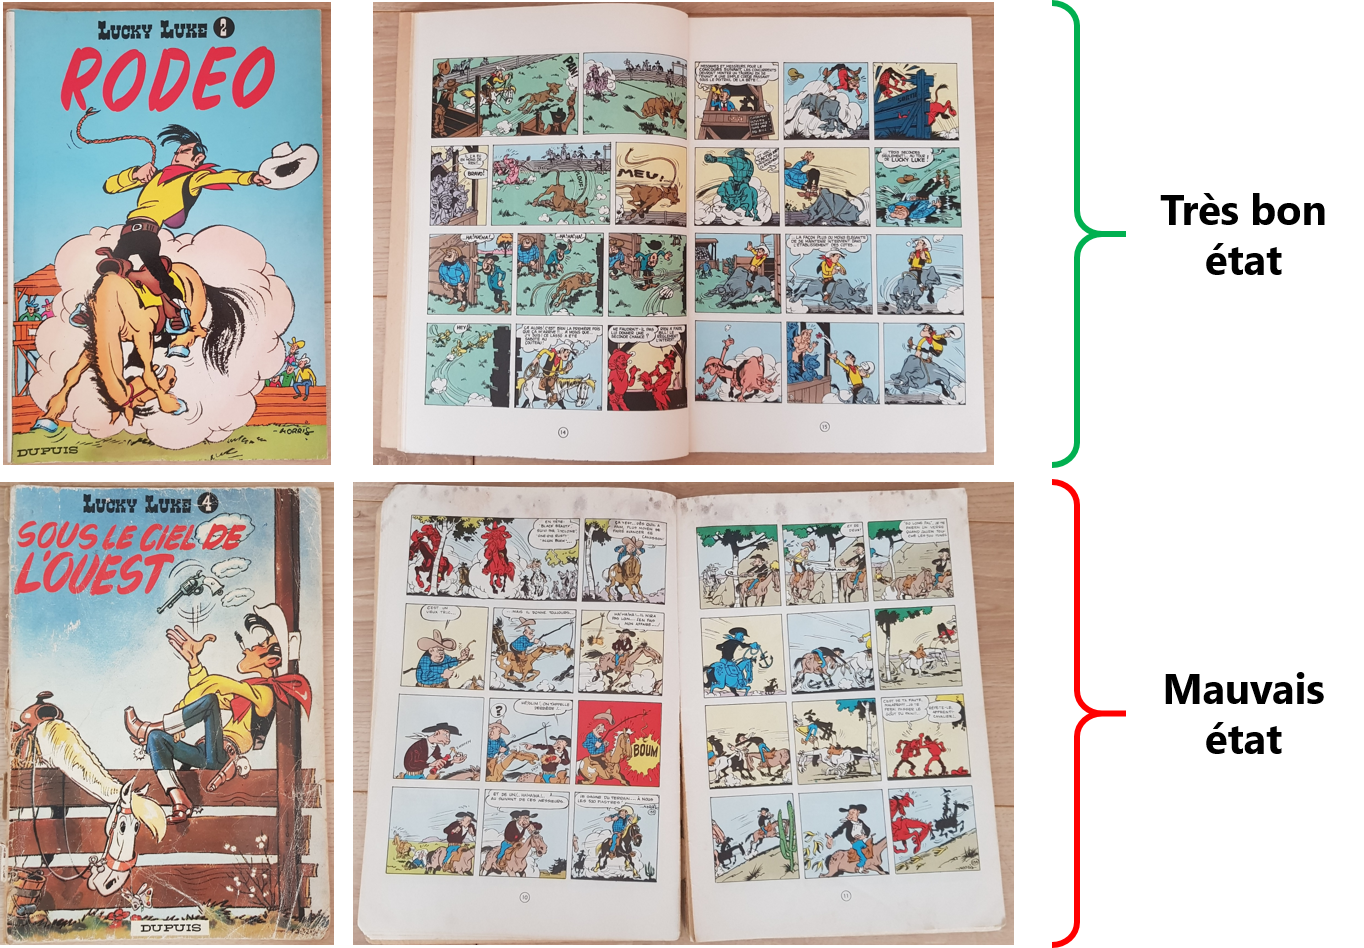
\includegraphics[width=0.80\textwidth]{figures/etatdelart-morris-1950-lucky-luke-2-1952-lucky-luke-4}
					\caption{
						Exemple d'annotation de l'état d'une \texttt{BD} (ici: \cite{morris-goscinny:1950:rodeo} et \cite{morris-goscinny:1952:sous-ciel-ouest}).
						La première est en très bon état (couverture comme neuve, tranches légèrement usées, pages intactes) tandis que la seconde est en mauvais état (couverture usée, dos abimée, traces sur les pages, ...).
					}
					\label{figure:2.1.2.B-PRESENTATION-ANNOTATION-EXEMPLES-CLASSIFICATION}
				\end{figure}
			\end{leftBarExamples}
			
			% Conclusion.
			Ainsi, si quelqu'un s'interroge sur l'état d'une bande dessinée en sa possession, ce modèle peut identifier l'état le plus probable d'après les exemples disponibles dans sa base d'apprentissage.
			
			% Autre cas d'usage similaire: Identifier la langue de la BD.
			\begin{leftBarInformation}
				De manière équivalente, il est possible de faire de la classification sur d'autres données, comme par exemple la classification de textes pour identifier la langue de l'ouvrage.
				Dans l'exemple ci-dessous, les catégories proposées sont "\texttt{Français}", "\texttt{Anglais}" et "\texttt{Allemand}", et la tâche d'annotation consiste ici à associer à chaque texte une catégorie de langue.
				\begin{center}
				\begin{tabular}{ c l }
					\textguillemets{\textit{
						Les cousins Dalton ont dévalisé la diligence.
					}} & $\implies$ \textcolor{colorSilverLakeBlue}{\texttt{Français}} \\
					\textguillemets{\textit{
						The Dalton cousins robbed the stagecoach.
					}} & $\implies$ \textcolor{colorDarkPastelGreen}{\texttt{Anglais}} \\
					\textguillemets{\textit{
						Die Dalton-Cousins haben die Postkutsche ausgeraubt.
					}} & $\implies$ \textcolor{colorDarkPastelRed}{\texttt{Allemand}}
				\end{tabular}
				\end{center}
			\end{leftBarInformation}
		
		
		%%% 2.1.2.C. Identification d'une bande dessinée à partir de sa couverture.
		\subsubsection{Identification d'une bande dessinée à partir de sa couverture.}
		\label{section:2.1.2.C-PRESENTATION-ANNOTATION-EXEMPLES-EXTRACTION}
			
			% Cas d'usage: identifier une bande dessinée
			Identifier une bande dessinée n'est pas toujours facile, et recopier l'ensemble des informations l'identifiant peut prendre du temps.
			Les libraires ou les collectionneurs désirant faire l'inventaire des ouvrages en leur possession peuvent ainsi y passer de nombreuses heures, avec le risque de faire des erreurs lors de l'inscription des bande dessinée dans leur registre.
			
			% Entrainer un modèle: extraction de caractères.
			Afin d'aider les collectionneurs, il est possible d'utiliser un modèle de \texttt{reconnaissance optique des caractères} (\texttt{OCR}) \footnote{
				Pour plus de détails sur l'\texttt{OCR}: voir la revue de \cite{berchmans-kumar:2014:optical-character-recognition} ou de \cite{awel-abidi:2019:review-optical-character}.
			} pour extraire automatiquement les informations importantes présentes sur les couvertures d'une \texttt{BD} à identifier.
			Pour entraîner un tel modèle, il est nécessaire d'avoir une base d'apprentissage contenant des exemples de pages de couverture avec la position et la valeur des informations pertinentes à extraire.
			La tâche d'annotation peut alors consister à renseigner pour chaque couverture de bande dessinée :
			\begin{itemize}
				\item la position des informations en l'encadrant sur l'image (avec un rectangle par exemple) ;
				\item la valeur écrite dans l'encadré sur l'image.
			\end{itemize}
			
			% Citation de l'exemple.
			Un exemple d'annotation de textes dans une image est disponible dans la \textsc{Figure~\ref{figure:2.1.2.C-PRESENTATION-ANNOTATION-EXEMPLES-EXTRACTION}}.
			%
			\begin{leftBarExamples}
				\begin{figure}[H]
					\centering
					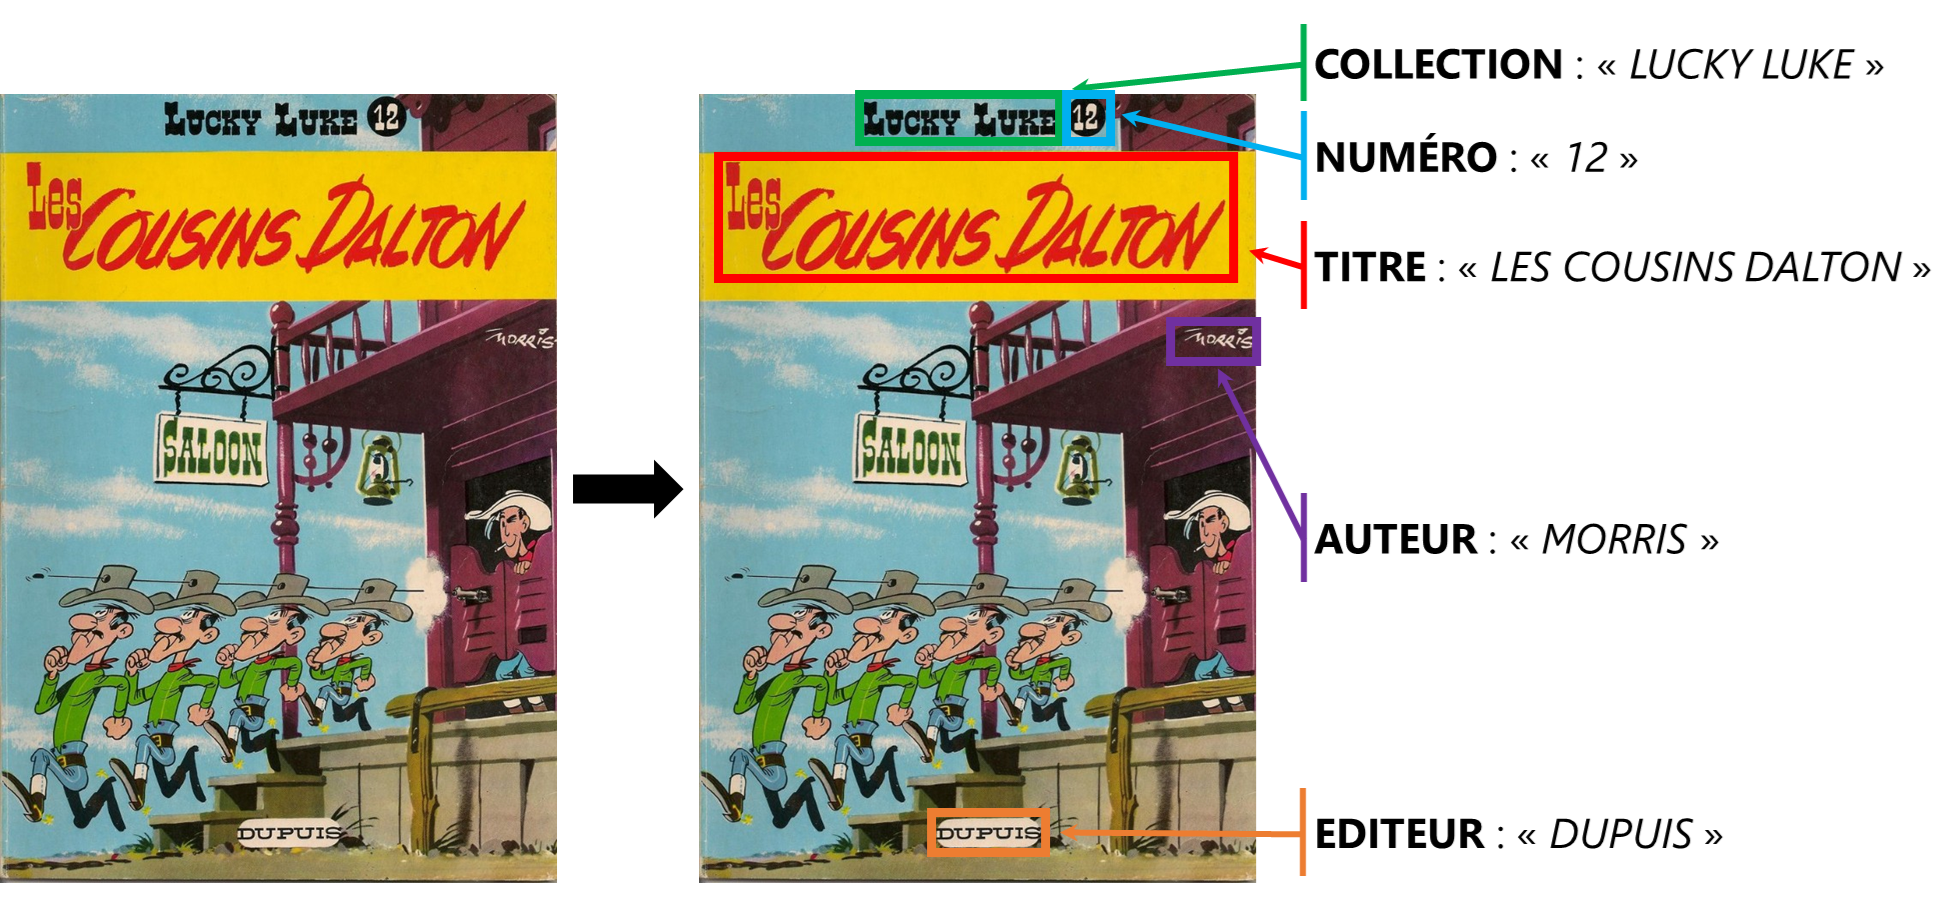
\includegraphics[width=0.80\textwidth]{figures/etatdelart-morris-1958-lucky-luke-12}
					\caption{
						Exemple d'annotation de textes présents sur la couverture d'une bande dessinée (ici: \cite{morris-goscinny:1958:cousins-dalton}).
						Les informations essentielles telles que la collection, le numéro, le titre, l'auteur et l'éditeur y sont présentes. 
					}
					\label{figure:2.1.2.C-PRESENTATION-ANNOTATION-EXEMPLES-EXTRACTION}
				\end{figure}
			\end{leftBarExamples}
			
			% Conclusion.
			Ainsi, si quelqu'un veut identifier une nouvelle bande dessinée, il peut interroger le modèle d'extraction de caractères pour récupérer les informations textuelles présentes dans la couverture, à l'image des exemples disponibles dans sa base d'apprentissage.
			
			% Autres cas d'usage: Extraire les information d'un texte.
			\setcounter{localCounterOfFootnoteValue}{\value{footnote}}
			\begin{leftBarInformation}
				De manière équivalente, il est possible de réaliser une \texttt{reconnaissance d'entités nommées (\texttt{NER})} \footnotemark pour extraire les informations citées dans un texte.
				Dans l'exemple ci-dessous, les types d'entités présentes sont "\texttt{personnage}", "\texttt{métier}", "\texttt{argent}", "\texttt{lieu}" et "\texttt{date}".
				La tâche d'annotation consiste ici à identifier la position et le type de chaque entité présente.
				
				\begin{quote}
					\textguillemets{\textit{
						$\textbf{\text{Lucky Luke}}_{\textcolor{colorDarkPastelRed}{\texttt{(personnage)}}}$, le $\textbf{\text{cow-boy}}_{\textcolor{colorDarkPastelPurple}{\texttt{(métier)}}}$ solitaire, a attrapé les $\textbf{\text{Dalton}}_{\textcolor{colorDarkPastelRed}{\texttt{(personnage)}}}$ à $\textbf{\text{Coyote Gulch}}_{\textcolor{colorCarrotOrange}{\texttt{(lieu)}}}$ et a touché $\textbf{\text{50.000\$}}_{\textcolor{colorSilverLakeBlue}{\texttt{(argent)}}}$ en les livrant au $\textbf{\text{pénitencier}}_{\textcolor{colorCarrotOrange}{\texttt{(lieu)}}}$. Ils se sont évadés le $\textbf{\text{jeudi suivant}}_{\textcolor{colorDarkPastelGreen}{\texttt{(date)}}}$.
					}}
				\end{quote}
			\end{leftBarInformation}
			% Rattraper les footnote.
				\stepcounter{localCounterOfFootnoteValue}
				\footnotetext[\value{localCounterOfFootnoteValue}]{
					Pour plus de détails sur la reconnaissance d'entités nommées (\texttt{NER}): voir les revues de \cite{goyal-etal:2018:recent-named-entity} ou de \cite{li-etal:2022:survey-deep-learning}.
				}
		
		
		%%% 2.1.2.D. Interprétation audio d'une bande dessinée.
		\subsubsection{Interprétation audio d'une bande dessinée.}
		\label{section:2.1.2.D-PRESENTATION-ANNOTATION-EXEMPLES-TRANSCRIPTION}
		
			% Cas d'usage: générer une lecture audio.
			Il est de plus en plus commun de trouver des livres disponibles avec une lecture audio.
			Ces audio-livres, réalisés par une personne ou synthétisés par l'ordinateur, peuvent être à visée éducative ou simplement disponibles pour le loisir.
			Dans le cadre de notre exemple sur le thème des bandes dessinées, peu d'entre elles disposent d'une lecture audio.
			Une idée serait donc d'interpréter une lecture audio de ces bandes dessinées en synthétisant la voix des doubleurs de leurs adaptations télévisées (ou simplement d'un narrateur si l'oeuvre n'a pas été portée à l'écran).
			
			% Entrainer un modèle: synthétiseur vocal.
			Dans le but de créer ces audio-\texttt{BD}, nous pourrions envisager d'utiliser des modèles de \texttt{synthèse vocale} (\texttt{TTS}) \footnote{
				Pour plus de détails sur la synthèse vocale: voir la revue de \cite{kothadiya-etal:2020:different-methods-review} ; voir un exemple d'architecture neuronale \texttt{end-to-end} dans \cite{mu-etal:2021:review-endtoend-speech}.
			} pour générer automatiquement la lecture des bulles d'une bande dessinée.
			Pour entraîner de tels modèles, il est nécessaire d'avoir une base d'apprentissage contenant des exemples d'audios prononcés par chacun des personnages (ici: les doubleurs de l'adaptation télévisée) avec la transcription de leur paroles pour chaque audio.
			La tâche d'annotation peut alors consister à renseigner le personnage et les paroles qu'il a prononcées.
			
			% Citation de l'exemple.
			Un exemple d'annotation phonétique est illustré dans la \textsc{Figure~\ref{figure:2.1.2.D-PRESENTATION-ANNOTATION-EXEMPLES-TRANSCRIPTION}}.
			%
			\begin{leftBarExamples}
				\begin{figure}[H]
					\centering
					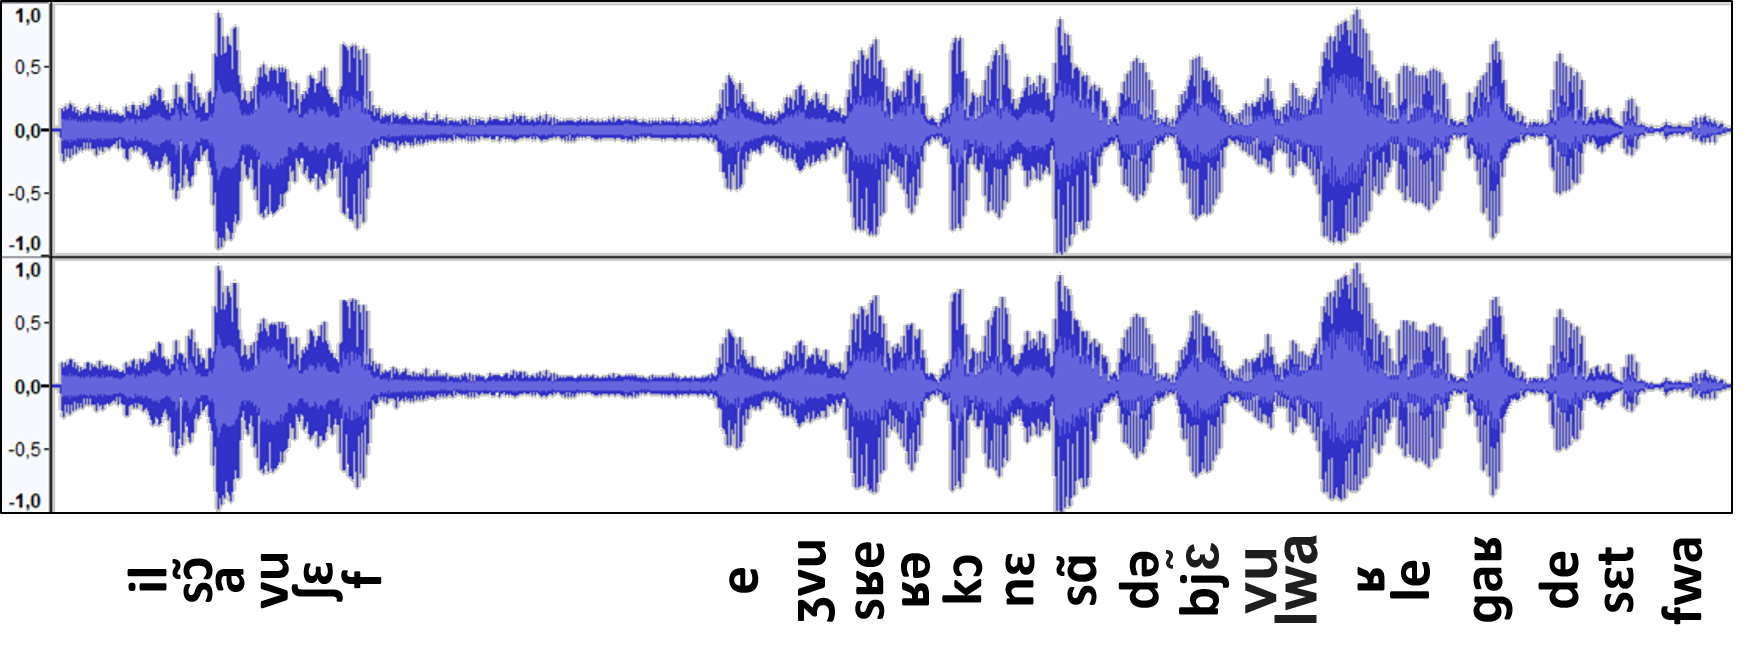
\includegraphics[width=0.95\textwidth]{figures/etatdelart-thebault-transcription}
					\caption{
						Exemple de paroles prononcées dans un audio.
						Ici, la voix de \textit{Lucky Luke} est interprétée par Jacques THEBAULT.
						Le texte annoté, c'est-à-dire celui prononcé dans l'audio, est  \textguillemets{\texttt{Ils sont à vous chef, et j'vous s'rai reconnaissant de bien les garder cette fois.}}.
						Les phonèmes en alphabet phonétique international associés à chaque séquence de l'audio sont disponibles si besoin.
						%[il sɔ̃ a vu ʃɛf, e ʒvu sʁe ʁə.kɔ.nɛ.sɑ̃ də bjɛ̃ vu.lwaʁ le ɡaʁ.de sɛt fwa].
					}
					\label{figure:2.1.2.D-PRESENTATION-ANNOTATION-EXEMPLES-TRANSCRIPTION}
				\end{figure}
			\end{leftBarExamples}
			
			% Conclusion.
			Ainsi, nous pourrions consulter le modèle de synthèse vocale d'un personnage (ici: celui de \texttt{Lucky Luke}) avec un nouveau texte à prononcer pour en obtenir une lecture audio dont la voix se rapproche des enregistrements de la base d'apprentissage (ici: celle de Jacques THEBAULT).
			
			% Autres cas d'usage: comuler OCR + Classification + TTS
			\begin{leftBarInformation}
				Nous pourrions compléter le cas d'usage
				(1) en extrayant automatiquement le texte d'une planche de \texttt{BD} par \texttt{OCR},
				(2) en détectant automatiquement le personnage prononçant la bulle de \texttt{BD} par classification,
				puis (3) en générant du texte à prononcer par le personnage par synthèse vocale.
				Bien entendu, la conception et l'enchaînement de ces différents modèles sont plutôt complexes, et chaque tâche de \textit{Machine Learning} demande ses propres données annotées pour construire une base d'apprentissage.
			\end{leftBarInformation}
			
			
		%%% Exemple: Annotation génération musicale
		% Generation de musique: \cite{hernandez-olivan-beltran:2023:music-composition-deep}
		%\begin{leftBarExamples}
		%	Annotation des paroles d'une chanson (\cite{woods:1971:poor-lonesome-cowboy}). \\
		%
		%	\begin{guitar}
		%		\textbf{Im A Poor Lonesome Cowboy}
		%		\textit{
		%			~~~~from \texttt{Lucky Luke - Daisy Town OST} ($1971$)
		%			~~~~composed by \texttt{Claude Bolling}
		%			~~~~performed by \texttt{Pat Woods}
		%		}
		%		\texttt{Intro}
		%		\textit{
		%			[D]Lonesome [D7]cowboy, [G]Lonesome [G7]cowboy, [D]You're a [Bm]long [Bm7]long [E]way from [A]home.
		%			[D]Lonesome cowboy, [G]Lonesome cowboy, [D]You've a [Bm]long [Bm7]long [E]way [A7]to [D]roam.
		%		}
		%		\texttt{Couplet}
		%		\textit{
		%			I'm a [D]poor lonesome cowboy, I'm a long long way from home,
		%			And this poor lonesome [F\#m]cowboy, Has got a [Em]long long way [A]to roam.
		%			Over [D]mountains and over [D7]prairies, From [G]dawn 'til day is [Em]done,
		%			My [Bm]horse and me keep [F\#]ridin', [G]into the [A]settin' [D]sun.
		%		}
		%		{ \center \textbf{...} }
		%	\end{guitar}
		%\end{leftBarExamples}
		
		
		%%% Exemple: Annotation étiquette gramaticale
		%\begin{leftBarExamples}
		%	Annotation des étiquettes grammaticales dans un texte.
		%	\begin{quote}
		%		\textguillemets{\textit{
		%			$\text{Les}_{\textcolor{colorDarkPastelPurple}{\texttt{(DET)}}}$
		%			$\text{dangereux}_{\textcolor{colorMinionYellow}{\texttt{(ADJ)}}}$
		%			$\text{Dalton}_{\textcolor{colorDarkPastelRed}{\texttt{(PROPN)}}}$
		%			$\text{se}_{\textcolor{colorCarrotOrange}{\texttt{(PRON)}}}$
		%			$\text{sont}_{\textcolor{colorDarkPastelGreen}{\texttt{(AUX)}}}$
		%			$\text{encore}_{\textcolor{colorSilverLakeBlue}{\texttt{(ADV)}}}$
		%			$\text{évadés}_{\textcolor{colorDarkPastelGreen}{\texttt{(VERB)}}}$
		%			$\text{de}_{\textcolor{colorDimGray}{\texttt{(ADP)}}}$
		%			$\text{prison}_{\textcolor{colorDarkPastelRed}{\texttt{(NOUN)}}}$
		%			$\text{et}_{\textcolor{colorBlack}{\texttt{(CCONJ)}}}$
		%			$\text{ils}_{\textcolor{colorCarrotOrange}{\texttt{(PRON)}}}$
		%			$\text{ont}_{\textcolor{colorDarkPastelGreen}{\texttt{(AUX)}}}$
		%			$\text{déjà}_{\textcolor{colorSilverLakeBlue}{\texttt{(ADV)}}}$
		%			$\text{dévalisé}_{\textcolor{colorDarkPastelGreen}{\texttt{(VERB)}}}$
		%			$\text{une}_{\textcolor{colorDarkPastelPurple}{\texttt{(DET)}}}$
		%			$\text{banque}_{\textcolor{colorDarkPastelRed}{\texttt{(NOUN)}}}$
		%			$\text{à}_{\textcolor{colorDimGray}{\texttt{(ADP)}}}$
		%			$\text{Daisy Town}_{\textcolor{colorDarkPastelRed}{\texttt{(PROPN)}}}$.
		%		}}\\
		%		%{ \center \scriptsize (
		%		%	Adjectif: {\textcolor{colorMinionYellow}{\texttt{(ADJ)}}} ;
		%		%	Adverbe: {\textcolor{colorSilverLakeBlue}{\texttt{(ADV)}}} ;
		%		%	Conjonction: {\textcolor{colorBlack}{\texttt{(CCONJ)}}} ;
		%		%	Déterminant: {\textcolor{colorDarkPastelPurple}{\texttt{(DET)}}} ;
		%		%	Nom: {\textcolor{colorDarkPastelRed}{\texttt{(NOUN)}}}, {\textcolor{colorDarkPastelRed}{\texttt{(PROPN)}}} ;
		%		%	Préposition: {\textcolor{colorDimGray}{\texttt{(ADP)}}} ;
		%		%	Pronom: {\textcolor{colorCarrotOrange}{\texttt{(PRON)}}}, ;
		%		%	Verbe: {\textcolor{colorDarkPastelGreen}{\texttt{(AUX)}}}, {\textcolor{colorDarkPastelGreen}{\texttt{(VERB)}}}.
		%		%)}
		%	\end{quote}
		%\end{leftBarExamples}
	
	
	%%%
	%%% Subsection 2.1.3: Bilan concernant la présentation de l'annotation.
	%%%
	\subsection{Bilan concernant la présentation de l'annotation}
	\label{section:2.1.3-PRESENTATION-ANNOTATION-BILAN}
	
	%%%
	%%% Conclusion.
	%%%
	\begin{leftBarSummary}
		\begin{todolist}
			% Définition de l'annotation.
			\item[\itemok] \textguillemets{\texttt{Annoter}} une donnée consiste à \textbf{ajouter un complément d'information} pour pouvoir mieux interpréter puis reproduire un phénomène.
			% Type d'annotation.
			\item[\itemok] Le type d'annotation à réaliser \textbf{dépend du problème à traiter} : régression, classification, extraction d'information, génération ou synthèse de données, ...
			% Corpus d'entraînement.
			\item[\itemok] L'ensemble des données annotées peut être utilisé pour concevoir un modèle d'\textguillemets{\texttt{apprentissage automatique}}: il est alors appelé \textguillemets{\texttt{corpus d'entraînement}}.
		\end{todolist}
	\end{leftBarSummary}
	
	
	%%%%%--------------------------------------------------------------------
	%%%%% Section 2.2: Organisation usuelle d'un projet d'annotation
	%%%%%--------------------------------------------------------------------
	%\newpage
	\section{Organisation usuelle d'un projet d'annotation}
\label{section:2.2-ORGANISATION-ANNOTATION}
	
	%%%
	%%% Introduction: Présenter l'organisation usuelle, les acteurs et le besoin d'outils.
	%%%
	Dans la section précédente, nous avons présenté l'importance d'avoir des données annotées pour entraîner d'un modèle de \textit{Machine Learning}.
	Maintenant, nous allons détailler l'organisation de cette tâche d'annotation, identifier les compétences nécessaires aux intervenants du projet ainsi que les fonctionnalités essentielles des outils de labellisation.
	
	
	%%%
	%%% Subsection 2.2.1: Étapes clés du cycle d'annotation.
	%%%
	\subsection{Étapes clés du cycle d'annotation}
	\label{section:2.2.1-ORGANISATION-ANNOTATION-ETAPES-CLES}
		
		%%% Introduction au cycle MATTER.
		Une référence en matière d'organisation de projet d'annotation est proposée par \cite{pustejovsky-stubbs:2012:natural-language-annotation} et est complétée dans \cite{stubbs:2013:methodology-using-professional}.
		Les auteurs y formalisent la conception et l'amélioration \textbf{cyclique} d'un modèle de \textit{Machine Learning}.
		Ce cycle est appelé cycle \texttt{MATTER} en référence aux six étapes de conception qui le composent : \textit{\textbf{M}odelize}, \textit{\textbf{A}nnotate}, \textit{\textbf{T}rain}, \textit{\textbf{T}est}, \textit{\textbf{E}valuate} et \textit{\textbf{R}evise}.
		Ces étapes sont schématisées en \textsc{Figure~\ref{figure:2.2.1-ORGANISATION-ANNOTATION-ETAPES-CLES-MATTER}} et nous détaillons chacune d'entre elles ci-dessous.
		%
		\begin{figure}[!htb]
			\centering
			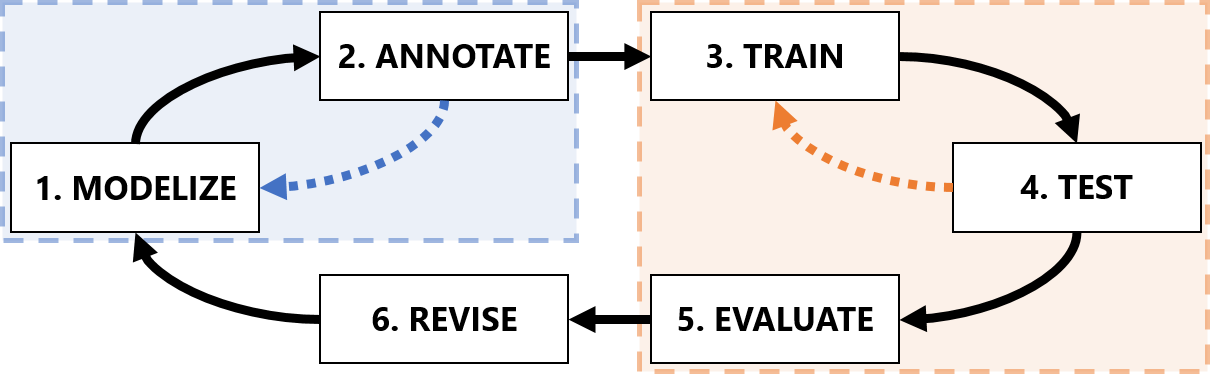
\includegraphics[width=0.95\textwidth]{figures/etatdelart-pustejovsky-2012-cycle-matter-mama-tt}
			\caption{
				Cycle \texttt{MATTER} structurant un projet d'annotation en six étapes principales: \textit{\textbf{M}odelize}, \textit{\textbf{A}nnotate}, \textit{\textbf{T}rain}, \textit{\textbf{T}est}, \textit{\textbf{E}valuate} et \textit{\textbf{R}evise}. \\
				Le carré bleu identifie le mini-cycle \texttt{MAMA} durant lequel la modélisation est adaptée en cours d'annotation,
				et le carré orange identifie le mini-cycle \textit{\textbf{T}rain}-\textit{\textbf{T}est} lors de la conception du modèle.
			}
			\label{figure:2.2.1-ORGANISATION-ANNOTATION-ETAPES-CLES-MATTER}
		\end{figure}
		%
		\begin{leftBarAuthorOpinion}
			Nous conseillons \cite{finlayson-erjavec:2016:overview-annotation-creation} pour son excellente revue de littérature qui détaille pas à pas le cycle \texttt{MATTER} tout en dressant la liste des points importants importants de chacune des étapes.
		\end{leftBarAuthorOpinion}
		
		%%% 2.2.1.A. Concevoir la base d'apprentissage (\textbf{M}odelize}, \textit{\textbf{A}nnotate}).
		\subsubsection{Concevoir la base d'apprentissage (\textit{\textbf{M}odelize}, \textit{\textbf{A}nnotate}).}
		\label{section:2.2.1.A-ORGANISATION-ANNOTATION-ETAPES-CLES-MODELIZE-ANNOTATE}
		
			%%% a. Collecte de données.
			Pour obtenir un bon modèle de \textit{Machine Learning}, il faut avoir une base d’apprentissage de qualité.
			Comme nous l'avons dit précédemment, cela commence par disposer d'un ensemble de données d'exemples qui représente fidèlement les différentes facettes du problème à modéliser (voir \textsc{Section~\ref{section:2.3.1.A-DEFIS-ANNOTATION-ASPECT-DONNEES-REPRESENTATIVITE}}).
			Une phase de \texttt{collecte} de données est alors organisée : cette collecte peut se baser sur des extractions de bases de données ou de sites internet à disposition, sur des enquêtes réalisées après d'utilisateurs finaux, ou encore sur les avis éclairés d'experts du problème.
			Certaines données peuvent aussi être artificiellement créées afin de compléter la collecte pour les aspects du problème difficile à observer.
			Une fois la collecte terminée, ces données brutes ont besoin d'être annotées pour pouvoir être exploitées. \\
			
			%%% b. Modelisation des données.
			
			% Importance de la modélisation.
			Afin de garantir la qualité de cette labellisation, \textbf{il est important de ne pas précipiter la tâche d'annotation}.
			En effet, l'objectif de cette tâche peut considérablement changer en fonction du phénomène à décrire, des données à disposition et de la finalité du modèle de \textit{Machine Learning} à entraîner.
			Il est donc fortement conseillé de bien \textbf{modéliser le problème}, c'est-à-dire de définir l'objectif de l'annotation, de clarifier en amont les modalités et les attendus de de cette tâche, et de préciser les règles que devront suivre les opérateurs.
			
			% Modélisation vs Spécification, Guide d'annotation et exemple.
			\cite{pustejovsky-stubbs:2012:natural-language-annotation} précisent notamment deux concepts importants de cette phase :
			\begin{itemize}
				\item la \textbf{modélisation} du problème, représentation de manière abstraite l'objectif à atteindre et décrivant ainsi la logique générale de l'annotation dans un \textit{schéma d'annotation} ;
				\item les \textbf{spécifications}, compilant dans un \textit{guide d'annotation} l'ensemble des règles concrètes à respecter pour mettre en application la modélisation.
			\end{itemize}
			Pour résumer cette distinction, la modélisation représente \textit{quoi} annoter (\textit{objectif, définition, valeurs possibles, ...}) alors que les spécifications décrivent \textit{comment} annoter (\textit{règles d'attribution, exemples et contre-exemple, règles de format, ...}).
			%
			\begin{leftBarExamples}
				% Exemple littérature.
				\cite{perrotin-etal:2018:annotation-actes-dialogue}, s'intéressant à la classification des conversations d'assistance en ligne en actes de dialogues, décrit son guide d'annotation dans \cite{asher-etal:2017:manuel-annotation-actes}.
				On y retrouve (1) la modélisation avec la présentation des étiquettes possibles à annoter, et (2) les spécifications avec les définitions concrètes, des exemples, des restrictions d'attribution, et la gestion des données non pertinentes. \\
				% Exemple BD.
				Dans nos exemples précédents (cf. \textsc{Section~\ref{section:2.1.2.B-PRESENTATION-ANNOTATION-EXEMPLES-CLASSIFICATION}}), nous avions modélisé le problème de classification de l'état d'une bande dessinée en quatre classes : "\texttt{Mauvais état}", "\texttt{Bon état}", "\texttt{Très bon état}", "\texttt{Neuf}".
				Il faudrait désormais rédiger les spécifications avec des définitions concrètes et quelques exemples  pour guider un annotateur, notamment pour l'aider à distinguer "\texttt{Bon état}" de "\texttt{Très bon état}".
			\end{leftBarExamples}
			
			% Quelques points importants sur la modélisation et exemples.
			Bien entendu, il n'est pas toujours facile de modéliser un problème ni de rédiger un guide d'annotation adéquat.
			Nous reviendrons plus tard sur les caractéristiques de cette tâche pouvant introduire de la complexité (voir \textsc{Section~\ref{section:2.3-DEFIS-ANNOTATION}}), mais il est important de souligner d'emblée les points élémentaires suivants :
			\begin{itemize}
				\item le besoin d'\textit{inter-opérabilité} et de \textit{ré-utilisabilité} : un projet d'annotation est toujours un investissement coûteux, il serait donc regrettable de perdre ou de ne pas pourvoir ré-utiliser ces données après ce projet.
				Par conséquent, il faut réfléchir au format des données ainsi qu'aux types de détails à fournir pour être sûr de pouvoir toujours exploiter les données si la modélisation évolue légèrement ou si un futur projet désire en bénéficier ;
				\item la balance entre \textit{généralité} et \textit{spécificité} : le niveau de détail requis dépend sans conteste du problème à modéliser : annoter trop peu de détail ne permet pas d'exploiter les données, mais en annoter trop peut rapidement complexifier la tâche et introduire des erreurs.
				Il faut donc trouver le juste milieu pour réaliser un travail de qualité qui ne soit pas trop pénible.
			\end{itemize}
			%
			\begin{leftBarExamples}
				Dans la classification de langue exposée en \textsc{Section~\ref{section:2.1.2.B-PRESENTATION-ANNOTATION-EXEMPLES-CLASSIFICATION}}, nous y avons annoté chaque texte grâce à trois classes : "\texttt{Français}", "\texttt{Anglais}" et "\texttt{Allemand}".
				\begin{itemize}
					% Exemple inter-opérabilité et de ré-utilisabilité.
					\item par soucis d'\textit{inter-opérabilité}, nous pourrions plutôt utiliser la norme ISO 639-3 (\cite{international-organization-for-standardization:2007:codes-representation-names}), soit les code "\texttt{fra}", "\texttt{eng}" et "\texttt{deu}", afin de standardiser l'annotation et ainsi pouvoir partager plus facilement les données labellisées avec d'autres projets ;
					% Exemple généralité et spécificité.
					\item afin de présenter un cas simple, nous avions proposé un modèle avec trois langues communes pour une bande dessinée d'origine belge.
					Toutefois, nous aurions pu \textit{spécialiser} davantage notre modèle en fonction des variations régionales en prenant en compte le Corse ("\texttt{cos}") ou le Wallon ("\texttt{wln}").
					Cette distinction peut être essentielle pour certaines saga publiées dans ces langues (comme \texttt{Astérix \& Obélix}), mais peut simplement être une source de confusion pour les autres (comme \texttt{Lucky Luke}).
				\end{itemize}
			\end{leftBarExamples}
			
			% Aide à la formalisation.
			\begin{leftBarInformation}
				Pour aider à concevoir le guide d'annotation et afin de se poser les bonnes questions, \cite{dipper-etal:2004:useradaptive-annotation-guidelines} dresse une liste de définitions et de recommandations à prendre en considération.
				Bien que ces conseils soient issus du traitement de données linguistiques, ils permettent d'identifier les sections importantes d'un guide d'annotation en fonction des attentes des différents acteurs de l'annotation (\textit{l'auteur, l'annotateur, l'explorateur de données, ...}) et de les rédiger en suivants certaines règles simples (\textit{introduire les objectifs, ordonner les règles par complexité, traiter en premier les cas par défaut, trier les valeurs des variables catégorielles par ordre alphabétiques, ...}).
				Des exemples reconnus pour leur bonne conception y sont notamment cités si vous avez besoin de référence pour concevoir votre propre guide.
			\end{leftBarInformation}
			
			
			%%% c. Annotation
			
			% Annotation en tant que telle.
			Lorsque le guide d'annotation est rédigé, la \textbf{phase de labellisation} peut commencer.
			Cette tâche est traditionnellement réalisée par un groupe d'experts choisi en fonction de leur connaissance sur le problème à caractériser (\textit{dans nos exemples sur les bandes dessinées, ce serait plutôt des libraires ou des collectionneurs}).
			Après leur avoir expliqué l'objectif de leur travail et partagé les règles de labellisation contenues dans le guide, les annotateurs se partagent les données et réalisent chacun une partie du corpus d'apprentissage.
			
			%%% d. Mini-cycle MAMA.
			
			\begin{leftBarInformation}
				% La théorie rencontre le réel.
				C'est généralement à ce stade que la théorie rencontre la pratique : certaines règles d'annotation peuvent difficilement être applicables, certains données peuvent être ambiguës ou hors-sujet, et deux annotateurs peuvent aussi avoir des avis différents sur l'annotation la plus adéquate.
				Il est aussi important de rappeler que l’annotation est un acte d'interprétation, et que les données sont donc labellisées par un humain dont l'avis n'est pas infaillible. 
				\cite{pustejovsky-stubbs:2012:natural-language-annotation} introduisent donc le premier sous-cycle \texttt{MAMA} en référence à la boucle entre \textit{\textbf{M}odelize} et \textit{\textbf{A}nnotate} qui peut avoir lieu tant que le guide d'annotation n'est pas adapté aux données manipulées ou que différents points de vues opposent les annotateurs.
				
				% Exemple.
				Par exemple, lors de l'annotation de la transcription audio en \textsc{Section~\ref{section:2.1.2.D-PRESENTATION-ANNOTATION-EXEMPLES-TRANSCRIPTION}}, il peut y avoir une voix principale accompagnée de plusieurs voix en arrière plan : une première adaptation du guide serait de clarifier si ces voix secondaires doivent être transcrites ou ignorées, voire si l'audio entier doit être considéré comme inexploitable.
				La réponse à cette question dépend bien entendu du phénomène à décrire et de l'objectif du modèle de \textit{Machine Learning} à entraîner : dans notre cas, nous pourrions probablement annoter uniquement la voix principale et ignorer l'audio si le bruit gène la compréhension.
			\end{leftBarInformation}
			
			%%% Finalité : la base d'apprentissage.
			À la fin de l'annotation (ou du cycle \texttt{MAMA}), le corpus d'entraînement est disponible pour concevoir un modèle de \textit{Machine Learning}.
		
		
		%%% 2.2.1.B. Concevoir le modèle (\textit{\textbf{T}rain}, \textit{\textbf{T}est}, \textit{\textbf{E}valuate}).
		\subsubsection{Concevoir le modèle (\textit{\textbf{T}rain}, \textit{\textbf{T}est}, \textit{\textbf{E}valuate}).}
		\label{section:2.2.1.B-ORGANISATION-ANNOTATION-ETAPES-CLES-TRAIN-TEST}
			
			%%% Apprentissage statistiques et importance du test.
			La phase d'entraînement du modèle est l'étape centrale de l'apprentissage automatique.
			Toutefois, comme l'apprentissage se base sur des méthodes statistiques, il est important d'introduire une phase de test et d'évaluation pour s'assurer des performances du modèle obtenu.
			Il est donc courant de considérer une boucle de raffinement du modèle tant que les performances n'ont pas atteint un seuil acceptable.
			
			%%% Train/Dev/Test.
			En pratique, il est d'usage de \textbf{créer trois jeux de données} à partir de la base d'apprentissage qui vient d'être annotée :
			\begin{itemize}
				% Train.
				\item le jeu d'\texttt{entraînement} :
				c'est sur cette partie des données que le modèle de \textit{Machine Learning} est conçu ;
				% Test.
				\item le jeu de \texttt{développement} (ou de validation) :
				le modèle entraîné est évalué sur ce jeu de donnée pour étudier son comportement, identifier ses forces et ses faiblesses, et ainsi permettre de le comparer à d'autres modèles entraînés pour cette même tâche ;
				% Dev.
				\item le jeu de \texttt{test} :
				le modèle retenu est évalué sur ce jeu de test pour déterminer ses performances réelles.
			\end{itemize}
			% \cite{van-der-goot:2021:we-need-talk}: définir un train/tune/dev/test
			
			%%% Evaluate.
			Ainsi, le modèle représente la connaissance présente dans le jeu \texttt{entraînement}, il est étudié puis affiné grâce au jeu de \texttt{développement}, et est finalement jugé en fonction de ses performances sur le jeu de \texttt{test}.
			Il est encore une fois difficile d'être exhaustif sur les analyses et les métriques à considérer car elles dépendent fortement du type de problème que le modèle tente de résoudre.
			Une métrique basique est l'\texttt{Accuracy} (ou taux de bonne prédiction), décrivant simplement le nombre de fois que le modèle a fait une bonne proposition sur l'ensemble du test.
			Suivant le problème et le type de données, d'autres métriques usuelles peuvent être utilisées comme le \texttt{MSE} (\textit{Mean Squared Error}) pour la prédiction de variables numérique (voir \cite{wallach-goffinet:1987:mean-squared-error}), le \texttt{f1-score} pour les variables catégorielles (voir \cite{sasaki:2007:truth-fmeasure}) ou le \texttt{WER} (\textit{Word Error Rate}) pour la transcription de textes (voir \cite{mccowan-etal:2005:use-information-retrieval}).
			Dans tous les cas, une règle d'or est de bien tenir à l'écart le jeu de test des deux autres jeux de données et qu'il ne soit pas utilisé dans la phase de développement pour éviter tout biais de sur-apprentissage\footnote{
				Pour plus de détails sur le sur-apprentissage: voir \cite{collins:2017:chapter-overfitting}
			}.

			%%% Finalité : le modèle et se sperformances.
			À la fin de ce cycle, le modèle de \textit{Machine Learning} est à disposition, et ses performances théoriques sont celles obtenues sur le jeu de test.
		
		%%% 2.2.1.C. Revoir la base d'apprentissage (\textit{\textbf{R}evise}).
		\subsubsection{Revoir la base d'apprentissage (\textit{\textbf{R}evise}).}
		\label{section:2.2.1.C-ORGANISATION-ANNOTATION-ETAPES-CLES-REVISE}
		
			% Besoin de réviser.
			Pour terminer cette boucle, il est parfois nécessaire d'envisager de corriger son modèle en remettant en cause la modélisation du problème et l'annotation des données.
			\cite{voormann-gut:2008:agile-corpus-creationa} formalisait en effet ce besoin de réviser la conception d'une base d'apprentissage en observant les lacunes du modèle obtenu, et \cite{pustejovsky-stubbs:2012:natural-language-annotation} évoque certaines révisions nécessaires de la modélisation dès la phase d'annotation (voir sous-cycle \texttt{MAMA} dans la \textsc{Figure~\ref{figure:2.2.1-ORGANISATION-ANNOTATION-ETAPES-CLES-MATTER}}).
			
			% Identifier un besoin de réviser.
			Divers pistes peuvent mener à une évolution de la base d'apprentissage :
			\begin{itemize}
				\item le modèle de \textit{Machine Learning} peut avoir de mauvaise performances, malgré son affinage lors de la phase de développement, ou peut manquer d'adaptabilité sur des données réelles ;
				\item la modélisation ou l'annotation peuvent devenir obsolète car le phénomène modélisé évolue dans le temps ;
				\item un cas d'usage non identifié jusqu'à présent nécessite de nouvelles données pour être pris en compte ;
				\item le modèle peut ne pas convenir aux utilisateurs finaux par manque d'ergonomie ou à cause d'une utilisation non prévue initialement ;
				\item ou encore, un nouvel algorithme de \textit{Machine Learning} a priori plus performant requiert une modélisation différente pour traiter le problème.
			\end{itemize}
			%
			\begin{leftBarExamples}
				% Exemple Inflation prix
				Pour illustrer nos propos, prenons la tâche d'estimation du prix d'une bande dessinée (cf. \textsc{Section~\ref{section:2.1.2.A-PRESENTATION-ANNOTATION-EXEMPLES-REGRESSION}}) : il se peut que les prix annoté sur les transactions ne soient plus d'actualité à cause de l'inflation, et que les données doivent être ré-annotées pour prendre en compte les nouvelles valeurs du marché.
				
				% Exemple ajouter une classe.
				D'autre part, la modélisation en tant que telle peut aussi être impacté : par exemple, dans le cadre de la classification de l'état d'une bande dessinée à partir d'une photo (cf. \textsc{Section~\ref{section:2.1.2.B-PRESENTATION-ANNOTATION-EXEMPLES-CLASSIFICATION}}), on pourrait constater à l'usage qu'il manque une catégorie "\texttt{Très mauvais état}" nécessaire pour trier d’emblée toute \texttt{BD} indigne à la vente.
				
				% Exemple OCR.
				Enfin, il est possible que le modèle se comporte mal sur certaines données.
				Par exemple lors de l'identification d'une bande dessinée à partir de sa couverture (cf. \textsc{Section~\ref{section:2.1.2.C-PRESENTATION-ANNOTATION-EXEMPLES-EXTRACTION}}), certains textes du décors pourrait être extrait à tord (comme le texte de la pancarte \textguillemets{\textit{Saloon}} dans la \textsc{Figure~\ref{figure:2.1.2.C-PRESENTATION-ANNOTATION-EXEMPLES-IMAGE-OCR}}).
				Il faudra peut-être adapter l'annotation pour identifier les textes à ne pas extraire (avec une classe de rebus par exemple).
			\end{leftBarExamples}
			
			% Conclusion.
			Nous bouclons ainsi le cycle \texttt{MATTER} qui préfigure le besoin d'une amélioration continue d'un modèle de \textit{Machine Learning} pour que celui-ci soit le plus adapté à son environnement d'utilisation.
	
	
	%%%
	%%% Subsection 2.2.2: Portraits des acteurs intervenant sur un projet d'annotation.
	%%%
	\subsection{Portraits des acteurs intervenant sur un projet d'annotation}
	\label{section:2.2.2-ORGANISATION-ANNOTATION-ACTEURS}
	
		% Introduction: grande diversité de métiers.
		Au cours du cycle \texttt{MATTER}, nous pouvons constater que divers acteurs interviennent pour concevoir la base d'apprentissage et entraîner un modèle de \textit{Machine Learning}.
		Cette diversité de métiers qui gravitent autour du traitement automatique des données semble difficile à détailler, tant à cause de leur grand nombre que de leurs subtiles différences.
		Pour avoir un aperçu, vous pouvez consulter les offres d'emplois du marché actuel (voir \cite{team-datascientest:2022:metiers-data-mieux} ou \cite{databird:2023:10-metiers-data}) ou certaines formations professionnelles (voir \cite{isoz:2017:decouvrir-metiers-data}) pour pouvoir faire la distinction entre \textit{data scientist}, \textit{data analyst}, \textit{data librarian}, \textit{data journalist}, \textit{data architect}, \textit{data engineer}, \textit{data steward}, \textit{data archivist}, ou encore \textit{machine learning engineer}...
		
		% Approche par compétences.
		Afin d'avoir une approche moins commerciale de ces métiers, nous proposons plutôt de dresser les compétences requises au diverses phases du cycle, à l'image de \cite{radovilsky-etal:2018:skills-requirements-business} qui présente les acteurs de la science des données grâce à quatre groupes de compétences :
		\begin{enumerate}
			% Business expert.
			\item les compétences \textbf{métiers} : elles sont liées aux connaissances et à l'expertise sur le phénomène à modéliser ou le problème à résoudre.
			Ce sont grâce à ces compétences qu'un acteur peut être apte à annoter une donnée ou à qualifier la pertinence de la prédiction d'un modèle de \textit{Machine Learning}.
			Les métier(s) associé(s) sont : l'\texttt{expert métier} (\textit{business expert}) ;
			% Data analyst.
			\item les compétences \textbf{analytiques} : elles concernent entre autres la modélisation du problème, la gestion des données, et les analyses statistiques sur les biais et les performances.
			Ce sont grâce à ses compétences qu'un acteur peut concevoir le guide d'annotation, estimer le taux d'accord inter-annotateurs, ou encore réaliser l'évaluation statistique d'un modèle de \textit{Machine Learning}.
			Les métier(s) associé(s) sont : l'\texttt{analyste des données} (\textit{data analyst}) ou le \texttt{scientifique des données} (\textit{data scientist}) ;
			% Data scientist.
			\item les compétences \textbf{techniques} : elles portent sur l'ingénierie autour du modèle de \textit{Machine Learning}, comme le choix du meilleur algorithme d'entraînement et réglage fin des hyper-paramètres, l'archivage des différentes versions du modèle ainsi que son déploiement dans un environnement de production.
			Les métier(s) associé(s) sont : le \texttt{scientifique des données} (\textit{data scientist}), l'\texttt{ingénieur en Machine Learning} (\textit{Machine Learning Engineer}) ou l'\texttt{architecte des des données} (\textit{data architecte}) ;
			% Projet leader.
			\item et les compétences en \textbf{gestion} ou en \textbf{communication} : elles permettent d'aborder le cadrage du projet et la définition des objectifs, ainsi que diverses aptitudes transverses comme l'établissement de rapports, la gestion de projet, la vérification des normes, ...
			Les métier(s) associé(s) sont : le \texttt{chef de projet} (\textit{project leader}) ou le \texttt{responsable de la protection des données} (\textit{data protection officer}).
		\end{enumerate}
		\begin{leftBarInformation}
			On peut compléter cette vision par compétences avec la vision donnée par \cite{fort:2017:experts-ou-foule}, selon laquelle il y a trois types d'experts lors d'un projet d'annotation :
			\begin{itemize}
				\item les \textbf{experts du corpus} de données, ayant par exemple les connaissances sur les bandes dessinées, s'approchant donc de compétences \texttt{métiers} ;
				\item les \textbf{experts de l'annotation}, ayant par exemple les connaissances sur l'annotation de textes dans une image, s'approchant donc de compétences \texttt{analytiques} ;
				\item et les \textbf{experts de la tâche} de \textit{Machine Learning}, ayant par exemple les connaissances sur les techniques d'\texttt{OCR}, s'approchant donc des compétences \texttt{techniques}.
			\end{itemize}
		\end{leftBarInformation}
		
		% Application au cycle \texttt{MATER}.
		Ainsi, durant le cycle \texttt{MATTER}, nous pouvons voir les compétences ci-dessus se compléter :
		\begin{enumerate}
			% Concevoir la base d'apprentissage.
			\item la conception de la \textbf{base d'apprentissage} (étapes \textit{\textbf{M}odelize} et \textit{\textbf{A}nnotate}) nécessite :
			\begin{itemize}
				\item des compétences de \texttt{gestion} pour cadrer l'objectif du modèle à entraîner, et ainsi définir l'objectif auquel doit répondre l'annotation de données ;
				\item des compétences \texttt{analytiques} pour proposer une modélisation stable du phénomène et un guide d'annotation précis pour limiter les biais de conception ;
				\item des compétences \texttt{métiers} pour vérifier que la proposition de modélisation est pertinente vis-à-vis du cas d'usage, mais aussi pour réaliser l'annotation des données.
			\end{itemize}
			% Concevoir le modèle.
			\item la conception du \textbf{modèle de \textit{Machine Learning}} (étapes \textit{\textbf{T}rain}, \textit{\textbf{T}est}, \textit{\textbf{E}valuate}) nécessite :
			\begin{itemize}
				\item des compétences \texttt{analytiques} pour gérer les jeux de données (\textit{entraînement, développement, test}) et évaluer les performances statistiques du modèle ;
				\item des compétences \texttt{techniques} pour manipuler l'écosystème de développement du modèle, régler les hyper-paramètres, versionner les changements, et planifier la distribution du modèle ;
				\item des compétences de \texttt{gestion} pour s'assurer du respect des normes et des caractères privée ou confidentielle de certaines données.
			\end{itemize}
			% Revoir la base d'apprentissage
			\item la \textbf{révision} de la base d'apprentissage (étape \textit{\textbf{R}evise}) nécessite :
			\begin{itemize}
				\item des compétences \texttt{métiers} pour identifier le manque de pertinence du modèle vis-à-vis de certains cas d'usage ;
				\item des compétences \texttt{analytiques} pour disserter des performances réelles du modèle face à des données de production et remettre en question les précédents choix de modélisation pour espérer améliorer le modèle.
			\end{itemize}
		\end{enumerate}
		
		% Remarque sur la distance entre métier et technique.
		On notera que les compétences transverses de \textbf{gestion} ou \textbf{communication} ne sont pas spécifiques à une étape du cycle \texttt{MATTER} (\textit{le cadrage, la gestion de projet et l'établissement de rapports étant réalisés tout au long du projet}), alors que les compétences \texttt{métier} et \texttt{techniques} n'interviennent généralement pas au même moment du cycle : autrement dit, des experts métiers croisent rarement des experts techniques et ne partagent donc que très rarement leurs connaissances.
	
	
	%%%
	%%% Subsection 2.2.3: Choix du logiciel d'annotation.
	%%%
	\subsection{Choix du logiciel d'annotation}
	\label{section:2.2.3-ORGANISATION-ANNOTATION-LOGICIELS}
	
		% Introduction: besoin d'un outil d'annotation.
		Pour terminer la description de l'organisation d'un projet d'annotation, attardons nous sur le choix du logiciel à utiliser pour labelliser les données.
		En effet, une diversité d'applications existent pour répondre aux besoins des annotateurs, mais il est important de noter que l'absence de certaines fonctionnalités essentielles risque de gêner le projet d'annotation, soit par l'introduction de biais, soit à cause de son manque d'inter-opérabilité avec d'autres tâches d'analyses ou d'annotation.
		
		% Liste des fonctionnalités importantes.
		Nous faisons référence à \cite{finlayson-erjavec:2016:overview-annotation-creation} pour dresser ci-dessous une liste des fonctionnalités principales (voire essentielles) d'un logiciel d'annotation.
		Pour simplifier la lecture, nous proposons de regrouper ces fonctionnalités dans les catégories suivantes :
		\begin{itemize}
			% Répondre à la \textbf{besoin d'annotation}.
			\item répondre à la \textbf{besoin d'annotation} :
				cette fonctionnalité est bien entendu obligatoire, car un logiciel ne permettant pas d'annoter vos données ne vous sera d'aucune utilité.
				Cette remarque semble être une évidence, mais nous nous permettons aussi d'étendre l’avertissement aux logiciels n'étant pas destinés à votre besoin d'annotation mais qui peuvent être détournés pour y répondre indirectement : de telles contournements peuvent introduire des biais et offrent généralement une expérience utilisateur assez médiocre ;
			% Intégrer le \texbf{guide d'annotation}.
			\item intégrer le \textbf{guide d'annotation} :
				ce livrable issu de la phase de modélisation du cycle \texttt{MATTER} doit être facilement accessible par les annotateurs car il contient la documentation et les instructions à appliquer lors de la labellisation.
				Les logiciels permettant d'intégrer directement ces définitions (\textit{avec exemples et contre-exemples}) ainsi que les règles d'annotation (\textit{comme les labels mutuellement exclusifs, les détails obligatoires, ...}) ont donc un net avantage ergonomique pour respecter la modélisation définie et ainsi garantir la qualité de la base d'apprentissage ; 
			% Autoriser l'\textbf{annotation multiple}.
			\item autoriser l'\textbf{annotation multiple} et l'\textbf{annotation multi-modale}: 
				il est fréquent de devoir annoter plusieurs une même donnée suivant des modélisations ou des paradigmes différents pour répondre à plusieurs cas d'usage (\textit{en prenant l'exemple de l'annotation d'images, on peut détourer les objets présents, identifier les textes inscrits, proposer une ou plusieurs catégories générales, proposer une description textuelle, ...}) ou encore de devoir annoter des données de natures différentes (\textit{en combinant texte, image et voix comme dans l'annotation des sous-titres d'une vidéo}).
				Les logiciels permettant ainsi de labelliser plusieurs informations et de manipuler plusieurs types de données sont donc plus facilement réutilisables et permettent de centraliser les annotations ;
			% Evaluer la \textbf{qualité de l'annotation}.
			\item évaluer la \textbf{qualité de l'annotation} :
				les erreurs d'annotation et les divergences d'opinions sur la modélisation sont inévitables.
				Il est donc appréciable de pouvoir les identifier, soit sur la base d'une comparaison directe entre deux annotateurs, soit en comparant avec l'annotation la plus probable issue d'une base de référence.
				Il peut aussi être intéressant de pouvoir calculer les scores d'accord inter-annotateurs sur un même échantillon de données pour estimer la qualité de la base d'apprentissage, de pouvoir corriger les erreurs lors de revues ou encore de trancher les cas de conflits apparent lors d'avis discordants ;
			% Permettre l'\textbf{inter-opérabilité} technique.
			\item permettre l'\textbf{inter-opérabilité} technique :
				il est toujours frustrant de ne pas pouvoir réutiliser des annotations d'un projet à l'autre car le format de stockage n'est pas compatible.
				Les logiciels prenant donc en considération plusieurs format de données (\textit{\texttt{PNG}/\texttt{JPG}, \texttt{MP3}/\texttt{WAV}, \texttt{XLSX}/\texttt{XML}/\texttt{JSON}, ...}) et respectant les standards de la tâche d'annotation lors des imports et exports sont donc à privilégier.
				De plus, il est conseillé de ne pas écrire directement les annotation dans les données (\textguillemets{\textit{\textbf{[Lucky Luke]}{\textcolor{colorDarkPastelRed}{\texttt{/(personnage)}}}, le \textbf{[cow-boy]}{\textcolor{colorDarkPastelPurple}{\texttt{/(métier)}}} solitaire, a ...}}), mais de les stocker dans des fichiers séparés pour garder une meilleure gestion et permettre les annotations multiples ;
			% Gérer le \textbf{flux de travail} et le \textbf{suivi de projet}.
			\item gérer le \textbf{flux de travail} et le \textbf{suivi de projet} :
				certaines fonctionnalités simples sont nécessaires à l'organisation de l'équipe d'annotation.
				Cela peut comprendre la répartition de la charge de travail, l'historisation des changements pour permettre les retours arrières, la possibilité d'émettre des appels d'aide ou d'écrire des commentaires sur les choix d'annotation, ou encore l'accompagnement des nouveaux annotateurs lors de leur monté en compétence ;
			% Favoriser le \textbf{confort de l'annotateur}.
			\item favoriser le \textbf{confort de l'annotateur} :
				le logiciel choisi sera utilisé au quotidien par l'équipe d'annotation, il semble donc essentiel de leur offrir une expérience utilisateur agréable pour réaliser leur tâche.
				Cela peut passer par une customisation de l'interface utilisateur afin d'être adapter à l'objectif d'annotation et par le paramétrage de raccourcis claviers.
				Simplifier l'accès et l'installation du logiciel peut aussi s'avérer utile pour favoriser son adoption, en favorisant par exemple les applications web permettant plus facilement le travail collaboratif ;
			% Permettre des \texbf{annotations et d'analyses avancées}.
			\item permettre des \textbf{annotations et d'analyses avancées} :
				la littérature scientifique regorge de techniques pouvant assister un annotateur dans son travail (\textit{pré-annotation, apprentissage actif, visualisation, interaction, ...}).
				Nous détaillons plusieurs de ces techniques dans la \textsc{Section~\ref{section:2.3-DEFIS-ANNOTATION}}.
		\end{itemize}
		
		% Quelques exemples.
		Considérant la diversité de cas d'usage d'annotation, une liste exhaustive des outils de labellisation n'est bien entendu pas possible.
		Nous tenons toutefois à présenter quelques exemples illustrés dans la \textsc{Figure~\ref{figure:2.2.3-ORGANISATION-ANNOTATION-LOGICIELS}}.
		%
		\begin{figure}[!htb]
			\centering
			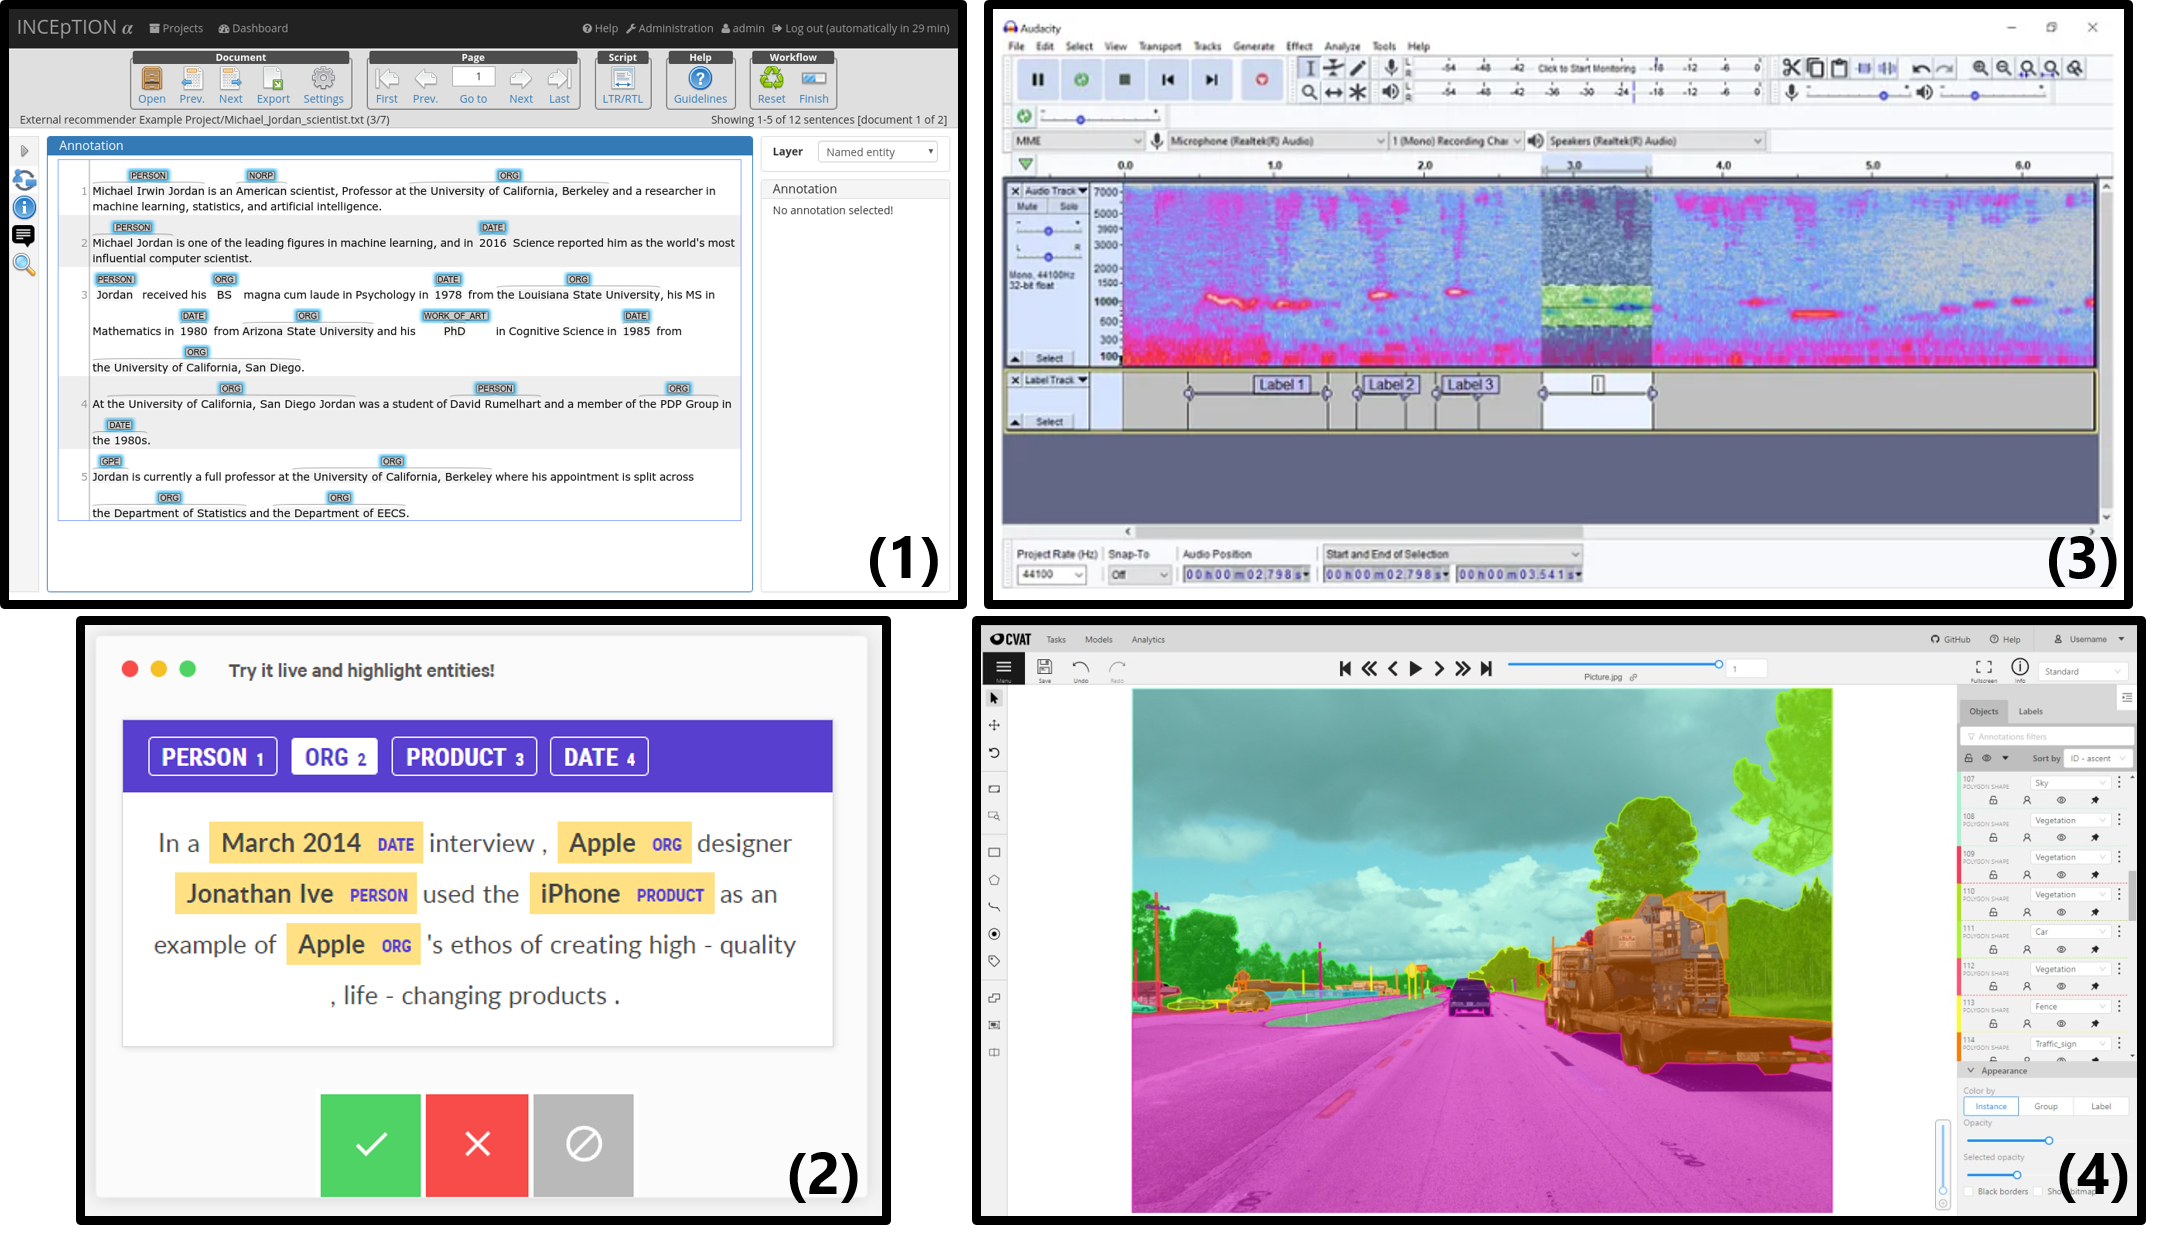
\includegraphics[width=0.95\textwidth]{figures/etatdelart-logiciel-exemples}
			\caption{
				Quatre exemples d'outils d'annotation :
				\textbf{(1)} \texttt{INCEpTION} pour le texte (\cite{klie-etal:2018:inception-platform-machineassisted}),
				\textbf{(2)} \texttt{prodigy} pour le texte ou l'image (\cite{montani-honnibal:2017:prodigy-modern-scriptable}),
				\textbf{(3)} \texttt{Audacity} pour l'audio (\cite{audacity-team:2000:audacity-free-audio}
				et \textbf{(4)} \texttt{CVAT} pour l'image (\cite{cvat.ai-corporation:2019:computer-vision-annotation}).
			}
			\label{figure:2.2.3-ORGANISATION-ANNOTATION-LOGICIELS}
		\end{figure}
		
		% Avis sur la sur-utilisation d'Excel.
		\begin{leftBarAuthorOpinion}
			De part notre expérience, nous constatons malheureusement que plusieurs projets industriels n'utilisent pas ou peu d'outils d'annotation dédiés, et se contentent plutôt d'outils rudimentaires comme des traitement de textes ou des tableurs tels que \texttt{Microsoft Excel} (\cite{microsoft-corporation:2018:microsoft-excel}).
			Une étude serait à mener pour étudier cette tendance et expliquer le manque d'intérêt porté aux outils spécialement conçus pour les tâches d'annotations.
			Peut-être que ces derniers s'adaptent mal aux particularités des divers projets industriels, expliquant ainsi l'utilisation d'outils simplistes mais flexibles. Ou alors est-ce par méconnaissance des difficultés et des bais potentiels de l'annotation que ces outils aux fonctionnalités avancées ne sont pas employés ?
		\end{leftBarAuthorOpinion}
	
	
	%%%
	%%% Subsection 2.2.4: Bilan concernant les nombreux défis de l'annotation.
	%%%
	\subsection{Bilan concernant l'organisation d'un projet d'annotation}
	\label{section:2.2.4-ORGANISATION-ANNOTATION-BILAN}
	
	%%%
	%%% Conclusion.
	%%%
	\begin{leftBarSummary}
		\begin{todolist}
			% MATTER.
			\item[\itemok] En général, un projet d'annotation est \textbf{organisé en cycle (\texttt{MATTER})} au cours duquel nous réalisons une modélisation abstraite des données que nous formalisons dans un guide (\textit{\textbf{M}odelize}), nous appliquons ce guide pour labelliser notre base d'apprentissage (\textit{\textbf{A}nnotate}), puis nous entraînons et testons un modèle de \textit{Machine Learning} (\textit{\textbf{T}rain}, \textit{\textbf{T}est} et \textit{\textbf{E}valuate}).
			Ensuite, l'évaluation du modèle peut mener à une révision de la modélisation des données en fonction des performances obtenues (\textit{\textbf{R}evise}) ;
			% Acteurs.
			\item[\itemok] Un tel projet d'annotation nécessite une \textbf{diversité de connaissances et de compétences} qui peuvent être réparties en quatre catégories : \texttt{métier}, \texttt{analytique}, \texttt{technique} et \texttt{gestion/communication} ;
			% Outils.
			\item[\itemok] Un tel projet nécessite aussi un \textbf{outil d'annotation dédié} possédant certaines fonctionnalités essentielles comme la possibilité d'\texttt{intégrer le guide} d'annotation, le besoin de \texttt{contrôler la qualité} des annotations, la capacité à réaliser des \texttt{annotation multiples ou multimodales}, ou encore l'assimilation d'éléments de \texttt{gestion de projet}.
		\end{todolist}
	\end{leftBarSummary}
	
	
	%%%%%--------------------------------------------------------------------
	%%%%% Section 2.3: Les nombreux défis de l'annotation
	%%%%%--------------------------------------------------------------------
	%\newpage
	\section{Les nombreux défis de l'annotation}
\label{section:2.3-DEFIS-ANNOTATION}

	%%%
	%%% Introduction: annoncer la complexité due (1) aux données (2) à la tâche et (3) aux humains.
	%%%
	
	Comme nous avons pu l'apercevoir dans les sections précédentes, le cycle d'annotation recèle de zones d'ombres pouvant introduire des complications ou des biais, explicites ou implicites, dans la conception d'une base d'apprentissage (\cite{baledent:2022:complexite-annotation-manuelle}).
	Pour aborder cette partie, nous alors voir :
	\begin{itemize}
		\item qu'il y a une forte pression sur la qualité des données constituant le corpus d'entraînement (cf. \textsc{Section~\ref{section:2.3.1-DEFIS-ANNOTATION-ASPECT-DONNEES}}) ;
		\item que ce standard de qualité entretien une complexité inhérente aux étapes de modélisation et d'annotation (cf. \textsc{Section~\ref{section:2.3.2-DEFIS-ANNOTATION-ASPECT-COMPLEXITE}}) ;
		\item et que cette complexité provoque des différences de comportements chez les annotateurs (cf. \textsc{Section~\ref{section:2.3.3-DEFIS-ANNOTATION-ASPECT-HUMAIN}}).
	\end{itemize}
	Nous profiterons aussi de ces points pour discuter des techniques et bonnes pratiques permettant de limiter les désagréments lors d'un projet d'annotation et identifier les freins lors de mises en application industrielles.
	
	
	%%%
	%%% Subsection 2.3.1: Défis concernant le besoin de qualité des données.
	%%%
	\subsection{Défis concernant le besoin de qualité des données}
	\label{section:2.3.1-DEFIS-ANNOTATION-ASPECT-DONNEES}
	
		% Introduction: Machine Learning = reproduire par l'exemple.
		Comme nous l'avons défini en \textsc{Section\ref{section:2.1.1.A-PRESENTATION-ANNOTATION-DEFINITION-MACHINE-LEARNING}}, l'\textguillemets{\texttt{apprentissage automatique}} regroupe un ensemble de techniques dont l'objectif est de reproduire une tâche \textbf{par l'exemple} : il est donc normal de porter une attention particulière aux données utilisées, car la qualité du modèle de \textit{Machine Learning} va fortement dépendre de la qualité de sa base d'apprentissage.
		Nous allons ici détailler trois défis actuels concernant le création d'un jeu de données.
		
		
		%%% 2.3.1.A. Problèmes de représentativité.
		\subsubsection{Problèmes de représentativité}
		\label{section:2.3.1.A-DEFIS-ANNOTATION-ASPECT-DONNEES-REPRESENTATIVITE}
			
			% Problème représentativité.
			Tout d'abord, accordons-nous sur le fait que certains phénomènes sont par essence complexes à représenter avec fidélité.
			C'est par exemple le cas avec :
			\begin{itemize}
				\item le traitement du langage :
			\end{itemize}
			\todo[inline]{SUITE A REDIGER}
			% \textsc{Section~\ref{section:2.1.2-PRESENTATION-ANNOTATION-EXEMPLES}}
			% donc collecte nombreuse ==> beaucoup de volume
			
			% exemple transaction BD: combinatoire des facteurs à prendre en compte
			% exemple du langage: argot, ...
			\begin{leftBarExamples}
			
			\end{leftBarExamples}
			
			
			% citation biber: prendre le temps de caractériser son problème et son JDD
			% data augmentation (attention aux biais), donc prenez le temps de bien décrire votre cas d'usage
			
			
			% donc beaucoup à annoter...
			% transfert d'apprentissage
			
		
		%%% 2.3.1.B. Problèmes de bruits.
			\subsubsection{Problèmes de bruits}
			\label{section:2.3.1.B-DEFIS-ANNOTATION-ASPECT-DONNEES-BRUITS}
			
				% 
		
		
		%%% 2.3.1.C. Problèmes de droits d'utilisation.
			\subsubsection{Problèmes de droits d'utilisation}
			\label{section:2.3.1.C-DEFIS-ANNOTATION-ASPECT-DONNEES-DROITS}
			
		
		
		%%%
		%%% Subsection 2.3.2: Défis concernant la complexité inhérente à la tâche d'annotation.
		%%%
		\subsection{Défis concernant la complexité inhérente à la tâche d'annotation}
		\label{section:2.3.2-DEFIS-ANNOTATION-ASPECT-COMPLEXITE}
			\todo[inline]{SECTION: À RÉDIGER}
		
		
		%%%
		%%% Subsection 2.3.3: Défis concernant les différences de comportements intra- et inter-annotateurs.
		%%%
		\subsection{Défis concernant les différences de comportements intra- et inter-annotateurs}
		\label{section:2.3.3-DEFIS-ANNOTATION-ASPECT-HUMAIN}
			\todo[inline]{SECTION: À RÉDIGER}
	
	
	%%%
	%%% Conclusion.
	%%%
	\begin{leftBarSummary}
		\begin{todolist}
			\item[\itemok] L'enjeu d'un projet d'annotation consiste à avoir des \textbf{données de qualité} qui soient représentatives du problème à traiter ;
			\item[\itemok] Or la tâche d'annotation et son exigence de qualité engendre de la \textbf{complexité}, et donc une \textbf{charge de travail élevée} ;
			\item[\itemok] Pour réguler cette charge de travail élevée, chaque opérateur va \textbf{adapter sa tâche} pour la rendre supportable, créant alors des \textbf{différences de comportement}.
		\end{todolist}
	\end{leftBarSummary}
	
	
	%%%%%--------------------------------------------------------------------
	%%%%% Section 2.4:
	%%%%%--------------------------------------------------------------------
	\section{Contexte du doctorat: assister la conception d'un jeu de données pour entraiter un agent conversationnel bancaire français}
	\label{section:2.4-CONTEXTE-DOCTORAT}
		\todo[inline]{SECTION: TITRE À TROUVER}
		\todo[inline]{SECTION: À CONFIRMER: \\
			- Chatbot: Task-oriented, entraîné avec intention et entitées et règles de dialogues \\
			- Données: pas de données linguistiques open source en français pour le domaine bancaire ==> besoin de créer le jeu de données \\
			- Modélisation: Phase longue en approche essai-erreur \\
			- Experts: Experts avec compétences métiers mais peu de connaissance en IA \\
			- Objectif du doctorat: trouver une alternative à ce processus manuel.
		}

%%%%%--------------------------------------------------------------------
%%%%% Chapitre: Clustering Interactif
%%%%%--------------------------------------------------------------------
\chapter[
	Proposition d'un \textit{Clustering Interactif} pour assister la tâche de modélisation
]{
	Proposition d'un \textit{Clustering Interactif} pour assister la tâche de modélisation d'un jeu de données textuelles
}
\label{chapter:3-CLUSTERING-INTERACTIF}
	
	% RÉSUMÉ DES ÉPISODES PRÉCÉDENTS: LA MODELISATION C'EST COMPLIQUÉ !
	Dans le chapitre précédent, nous avons vu les points essentiels suivants :
	%
	\begin{leftBarImportantGreen}
		\begin{todolist}
			% Importance de la modélisation. Mais modélisation complexe. Donc organisation généralement en cycle.
			\item[\itemok] L'étape de modélisation est nécessaire pour définir les objectifs et les règles d'un projet d'annotation ;
			or cette étape rencontre de nombreux défis qui la rendant particulièrement laborieuse (\textit{complexité intrinsèque du phénomène, subjectivité des opérateurs, différences de comportements, ...}).
			ainsi, la modélisation est régulièrement révisée (cycle \texttt{MATTER}).
			% Conception de chatbot task-oriented correspond à ce problème : phénomène complexe, modélisation complexe, experts mal intégrés.
			\item[\itemok] La modélisation de textes en intentions pour entraîner un assistant conversationnel orienté par tâches n'échappe pas à ce constat, notamment à cause de la complexité du langage naturel, de la diversité d'intentions de dialogue à représenter, et de la pression sur le contrôle du comportement de l'assistant.
			% Besoins d'experts ; Interventions complexes ; Tâche pénible et couteuse.
			\item[\itemok] Dans un cadre industriel, des experts métiers sont responsables de la modélisation et de l'annotation des données spécifiques ou confidentielles de l'entreprise ;
			or ces interventions requièrent des compétences analytiques et techniques dont les experts métiers ne disposent pas forcément ;
			de ce fait, la manipulation d'une modélisation abstraite de leurs connaissances est alors vécue comme une tâche pénible, nécessitant un grand nombre de formations et organisée sous la forme d'ateliers en mode essai-erreur.
		\end{todolist}
	\end{leftBarImportantGreen}
	
	% ANNONCE DU BUT DU CHAPITRE: MA CONTRIBUTION !
	Dans cette partie, nous cherchons une alternative à cette organisation traditionnelle, et nous proposerons une méthodologie d'annotation basée sur un \texttt{Clustering Interactif} visant à remplir un double objectif :
	%
	\begin{leftBarImportantRed}
		\begin{todolist}
			% 1. Efficacité de création du trainset.
			\item Permettre d'assister la modélisation et l'annotation des données pour créer plus efficacement une base d'apprentissage destinée à la classification d'intentions d'un assistant conversationnel ;
			% 2. Efficacité d'intervention d'un expert.
			\item Redéfinir les tâches et les objectifs des différents acteurs afin de rester au plus proche de leurs compétences réelles, particulièrement en ce qui concerne l'intervention des experts métiers du projet.
		\end{todolist}
	\end{leftBarImportantRed}
	
	% Référence articles.
	\begin{leftBarInformation}
		Cette proposition de méthode a été l'objet d'une présentation à la conférence \texttt{EGC (Extraction et Gestion des Connaissances)} (\cite{schild-etal:2021:conception-iterative-semisupervisee} et (\cite{schild-etal:2021:concevoir-assistant-conversationnel}), et d'une extension dans le journal \texttt{IJDWM (International Journal of Data Warehousing and Mining)}~(\cite{schild-etal:2022:iterative-semisupervised-design}).
		Nous reprenons ici certains des éléments présentés avec quelques détails supplémentaires.
	\end{leftBarInformation}

	% TABLE DES MATIÈRES DU CHAPITRE
	\minitoc


	%%%%%--------------------------------------------------------------------
	%%%%% Section 3.1: Intuitions à l'origine d'un \textit{Clustering Interactif}.
	%%%%%--------------------------------------------------------------------
	%\newpage
	%\vspace{2cm}
	\section{Intuitions à l'origine d'un \textit{Clustering Interactif}}
\label{section:3.1-INTUITIONS-ORIGINES}

	Tout d'abord, détaillons trois intuitions qui nous ont permis de concevoir notre méthodologie d'annotation.
	
	
	%%%
	%%% Subsection 3.1.1. Utiliser une approche non-supervisées pour créer une modélisation.
	%%%
	\subsection{Utiliser une approche non-supervisées pour créer une modélisation}
	\label{section:3.1.1-INTUITIONS-ORIGINES-NON-SUPERVISEES}
	
		%%% Possibilité d'utilisé des regroupements non supervisés.
		Dans le but d'assister la phase de modélisation des données, une piste intéressante revient à déléguer cette tâche à la machine.
		En effet, grâce à une \textbf{classification non-supervisés (\textit{clustering})}, un algorithme peut regrouper les données en fonction de leur similarité intrinsèque et ainsi suggérer une modélisation intentions.
		%%% Quelques exemples communs: KMeans, Hiérarchique, Spectral, DBScan, Affinity propagation, ...
		Plusieurs algorithmes et méthodes connus peuvent être utilisés :
		
		\begin{itemize}
			% KMeans.
			\item Le \textbf{\textit{clustering} \texttt{KMeans}} (\cite{macqueen:1967:methods-classification-analysis}) :
			Cette méthode se repose sur la minimisation de l'inertie intra-classes en attribuant chaque donnée au barycentre de \textit{cluster} le plus proche.
			Cette approche est l'une des plus répandues en raison de sa simplicité et de sa rapidité de calcul ;
			% Hiérarchique.
			\item Le \textbf{\textit{clustering} hiérarchique} (\cite{murtagh-contreras:2012:algorithms-hierarchical-clustering}) :
			Cette méthode revient à fusionner itérativement les données les plus similaires dans un nouveau \textit{cluster}.
			Plusieurs liens de similarité peuvent être implémentés (\textit{le lien \texttt{single} fusionnant les deux \textit{clusters} ayant les frontières les plus proches, le lien \texttt{complete} fusionnant les deux \textit{clusters} ayant les frontières opposées les plus proches, le lien \texttt{average} fusionnant les deux \textit{clusters} ayant les barycentres les plus proches et le lien \texttt{ward} fusionnant les deux \textit{clusters} qui donneront le prochain \textit{cluster} le plus compact}) ;
			% Spectral.
			\item Le \textbf{\textit{clustering} spectral} (\cite{ng-etal:2002:spectral-clustering-analysis}) :
			Cette méthode consiste à modéliser la matrice de similarité entre les données par ses vecteurs propres puis de regrouper ces derniers à l'aide d'un \texttt{KMeans}.
			Cette approche permet d'obtenir des \textit{clusters} aux formes complexes ;
			% DBScan.
			\item Le \textbf{\textit{clustering} \texttt{DBScan}} (\cite{ester-etal:1996:densitybased-algorithm-discovering}) :
			Cette méthode utilise la densité de données dans l'espace pour identifier des regroupements.
			Cette approche permet de découvrir des \textit{clusters} aux formes complexes si leur densité est suffisante.
			\item ...
		\end{itemize}
		
		%%% Cependant, il y a des limites.
		Cependant, ces algorithmes non-supervisés font régulièrement face à un ensemble de difficultés qui pénalisent leur utilisations.
		En effet, ces méthodes ont souvent du mal à traiter des données de grandes dimensionnalités ou en grand nombre (\cite{steinbach-etal:2004:challenges-clustering-high}), la présence de bruits peut rapidement perturber le fonctionnement d'un algorithme (\cite{yang-wang:2004:competitive-algorithms-clustering}), et certains \textit{clusters} aux géométries complexes peuvent être difficiles à identifier (\cite{kriegel-etal:2011:density-based-clustering}).
		De plus, le choix de certains hyperparamètres de ces méthodes n'est pas toujours simple, surtout en ce qui concerne le nombre de clusters, la méthode d'initialisation ou la mesure de distance à utiliser (\cite{agarwal-etal:2011:issues-challenges-tools}).
		Enfin, toutes ses difficultés se retrouvent dans le traitement du langage naturel, notamment à cause de la taille de vocabulaire important, de la présence de nombreux bruits et de la vaste diversité et complexité de thématiques pouvant y être abordés.
		\begin{leftBarInformation}
			La revue de \cite{xu-tian:2015:comprehensive-survey-clustering} détaille plusieurs algorithmes de \textit{clustering}, en fonction de leurs forces et faiblesses sur les points mentionnés ci-dessus.
		\end{leftBarInformation}
		
		% Conclusion : souvent jugés peu pertinents par les experts métiers.
		Ainsi, toutes ces limites étayent le fait qu'\textbf{un résultat brut d'une classification non supervisées est généralement perçu comme peu pertinent par les experts métiers}.
		Il est donc nécessaire d'introduire une intervention humaine dans le processus pour guider le fonctionnement d'un algorithme de \textit{clustering}.
		
	
	%%%
	%%% Subsection 3.1.2. Corriger l'approche non-supervisée avec une annotation de contraintes.
	%%%
	\subsection{Corriger l'approche non-supervisée avec une annotation de contraintes}
	\label{section:3.1.2-INTUITIONS-ORIGINES-SEMI-SUPERVISEES}
	
		%%% Proposition d'ajouts de contraintes pour corriger un \textit{clustering}.
		Une variante aux approches non-supervisées consiste à demander à un humain certaines informations nécessaires à leur amélioration nous considérons donc les \textbf{approches semi-supervisées}.
		Une manière efficace d'introduire les connaissances d'un expert dans le processus est l'ajout de contraintes.
		
		%%% Plusieurs types de contraintes.
		\cite{lampert-etal:2018:constrained-distance-based} rappelle qu'il peut y avoir deux types de contraintes :
		\begin{itemize}
			\item les \textbf{contraintes sur les données} : on parle alors principalement des contraintes binaires \texttt{MUST-LINK} et \texttt{CANNOT-LINK} décrivant si deux données doivent ou ne doivent être dans un même clusters (\cite{wagstaff-cardie:2000:clustering-instancelevel-constraints})
			\item les \textbf{contraintes sur les \textit{clusters}} : ces contraintes peuvent concerner le nombre de \textit{clusters} à trouver, leur taille minimale ou maximale, la distance minimale de séparation de leurs frontières, ...
		\end{itemize}
		
		% Nous choississons plutôt les contraintes sur les données.
		Bien que d'autres méthodes permettent d'insérer des contraintes (heuristiques non-supervisées, transferts de connaissances préalables), nous nous concentrons ici sur l'ajout manuel par un expert.
		Comme cet expert n'a a priori pas de connaissances techniques ou analytiques, ce dernier aurait du mal à manipuler des contraintes sur les \textit{clusters}.
		Toutefois, ses connaissances métiers lui permettent de caractériser facilement la similarité entre deux données, et donc de décrire des contraintes de type \texttt{MUST-LINK} et \texttt{CANNOT-LINK} en répondant à la question : \textguillemets{\textit{est-ce les deux données traite du même cas d'usage ?}}.
		
		\begin{leftBarAuthorOpinion}
			La pierre angulaire de la méthode que nous proposons en \textsc{Section~\ref{section:3.2-DESCRIPTION-THEORIQUE}} repose notamment sur le fait qu'il est difficile pour un expert métier de classer une question suivant une modélisation abstraite prédéfinie : cela l'éloigne de ses compétences métiers initiales, nécessite en contre-partie de nombreuses formations, et introduit de nombreuses erreurs d'annotations.
			De fait, il semble plus adéquat de demander à l'expert métier de discriminer deux questions sur la base de leurs similarité de cas d'usage métier.
		\end{leftBarAuthorOpinion}
		
		
		%%% Quelques exemples communs : COP KMeans, Hiérarchique, SPEC Spectral, C-DBScan, ...
		Parmi les algorithmes de \textit{clustering} sous contraintes connus, nous disposons des adaptations suivantes :
		
		\begin{itemize}
			% KMeans.
			\item Le \textbf{\textit{clustering} \texttt{KMeans} sous contraintes} comme \texttt{COP-KMeans} (\cite{wagstaff-etal:2001:constrained-kmeans-clustering}) :
			Dans cette version, l'attribution d'une donnée se fait au \textit{cluster} dont le barycentre est le plus proche et où aucune contraintes n'est violée.
			Cette adaptation est relativement simple à mettre en oeuvre, mais elle peut mener à des cas de blocage où plus aucun \textit{cluster} n'est accessible à cause de violation de contraintes (il est possible d'adapter l'algorithme en créant un nouveau \textit{cluster}) ;
			% Hiérarchique.
			\item Le \textbf{\textit{clustering} hiérarchique sous contraintes} (\cite{davidson-ravi:2005:agglomerative-hierarchical-clustering}) :
			Dans cette version, les données liées par des contraintes \texttt{MUST-LINK} sont d'abord fusionnées, puis le processus agglomératif commence en prenant garde de ne pas fusionner des \textit{clusters} ayant des contraintes \texttt{CANNOT-LINK} entre eux.
			Cette adaptation est très simple à mettre en oeuvre car il suffit d'adapter le calcul de distance entre \textit{clusters} ;
			% Spectral.
			\item Le \textbf{\textit{clustering} spectral sous contraintes} (\cite{kamvar-etal:2003:spectral-learning}) :
			Dans cette version, les coefficients de la matrice de similarité sont forcés à $0$ (respectivement $1$) si deux données sont liées par une contrainte \texttt{CANNOT-LINK} (respectivement \texttt{MUST-LINK}).
			Cette adaptation demande peu d'effort pour être mise en oeuvre, mais des modifications aussi drastiques de la matrice de similarité peut entraîner des changements imprévisibles de comportements ;
			% DBScan.
			\item Le \textbf{\textit{clustering} \texttt{DBScan} sous contraintes} comme \texttt{C-DBScan} (\cite{ruiz-etal:2010:densitybased-semisupervised-clustering}) :
			Dans cette version, la densité des données ainsi que les contraintes \texttt{CANNOT-LINK} sont utilisées pour identifier des clusters locaux qui seront ensuite fusionnés à l'aide des contraintes \texttt{MUST-LINK}
			Cette adaptation est plus compliquée à réaliser car elle change légèrement le fonctionnement interne d'exploration de la densité de l'espace de données.
			\item ...
		\end{itemize}
		
		Ces algorithmes de \textit{clustering} sous contraintes sont ainsi plein de potentiels : ils sont en effet capable de tirer parti de la similarité intrinsèque des données et des contraintes judicieusement placées de l'expert pour segmenter les données de manière adéquate et ainsi proposer une modélisation pertinente.
		\begin{leftBarExamples}
			On peut citer \cite{lampert-etal:2019:constrained-distance-based} où l'annotation de contraintes par un expert d'identifier efficacement dans objets dans une image satellite.
		\end{leftBarExamples}
		
		%%% Cependant, ils peuvent demander énorméments de contraintes : N^2 !
		Cependant, pour un jeu de données de taille $N$, il y a $N^2$ possibilités de contraintes à ajouter.
		L'estimation du placement des contraintes les plus appropriées et les plus efficaces pour corriger le \textit{clustering} semble donc être un problème \texttt{NP}-complexe.
		De plus, si ce choix peut être visuel pour des images (comme dans l'exemple cité ci-dessus), il ne l'est pas pour des données textuelles dont la diversité et la complexité sont difficiles à appréhender.
		Il est donc important d'assister l'expert métier à disposer ses contraintes afin de maximiser son impact dans la correction du \textit{clustering}.
		
	
	%%%
	%%% Subsection 3.1.3. Tirer parti des avantages de l'apprentissage actif pour optimiser les interactions Homme/machine.
	%%%
	\subsection{Tirer parti des avantages de l'apprentissage actif pour optimiser les interactions Homme/machine}
	\label{section:3.1.3-INTUITIONS-ORIGINES-APPRENTISSAGE-ACTIF}
	
		% Utiliser l'apprentissage actif.
		Une dernière piste intéressante est celle de l'apprentissage actif (\textit{active learning}, voir \cite{settles:2010:active-learning-literature}) : celle-ci prône les interactions Homme/machine comme moyen d'atteindre un objectif qu'aucun en peut atteindre séparément.
		% Liste d'interactions possibles avec le résultat, avec les hyperparamètres, avec des initaitives de la machine, ...
		\cite{bae-etal:2021:interactive-clustering-comprehensive} liste par exemple un ensemble d'interactions possibles avec un algorithme de \textit{clustering} : celles-ci peuvent concerner la manipulation et l'adaptation des résultats, l'adaptation des hyperparamètres des algorithmes, mais aussi des initiatives de la machine pour préparer la réalisation d'une tâche.
		
		% Nous sommes intéresser par la sélection optimale de contraintes à annoter
		Dans notre cas, nous nous intéressons en particulier aux initiatives de la machines pour identifier la liste des contraintes à annoter pour corriger ou confirmer efficacement un résultat de \textit{clustering}.
		Cela peut se faire par exemple à l'aide d'une heuristique sélectionnant les parties les moins sûres de la segmentation.
	
	%%%
	%%% Conclusion.
	%%%
	\begin{leftBarSummary}
		Dans cette partie, nous avons exposés les intuitions suivantes :
		\begin{todolist}
			% Pression sur la qualité.
			\item[\itemok] La phase de modélisation des données peut être déléguée à la machine en employant des algorithmes de classification non-supervisée (\textit{clustering}) ;
			\item[\itemok] Pour corriger le fonctionnement d'un algorithme de \textit{clustering} et ainsi améliorer la pertinence de ses résultats, l'expert peut ajouter des contraintes binaires sur les données (\texttt{MUST-LINK} et \texttt{CANNOT-LINK}, \textit{clustering} sous contraintes) ;
			\item[\itemok] Dans le but d'ajouter des contraintes de manière efficace, il est possible d'interagir avec la machine afin de maximiser l'impact de l'intervention de l'expert (\textit{active learning}).
		\end{todolist}
	\end{leftBarSummary}


	%%%%%--------------------------------------------------------------------
	%%%%% Section 3.2: Description théorique de notre \textit{Clustering Interactif}
	%%%%%--------------------------------------------------------------------
	\newpage
	%\vspace{2cm}
	\section{Description de notre \textit{clustering} interactif.}
\label{section:3.2-DESCRIPTION-THEORIQUE}

	Sur la base des intuitions que nous venons de détailler, nous proposons la méthode suivante dans le but d'assister la modélisation et l'annotation d'une collecte de données brutes en une base d'apprentissage nécessaire à l'entraînement d'un assistant conversationnel.
	
	%%%
	%%% Subsection 3.2.1. Description générale.
	%%%
	\subsection{Description générale}
	\label{section:3.2.1-DESCRIPTION-THEORIQUE-GENERALE}
	
		% Présentation succinte.
		\textbf{Notre méthode d'annotation}, que nous appelons \textguillemets{\texttt{Clustering Interactif}}, \textbf{repose sur l'alternance successive entre deux phases clefs} (voir \textsc{Figure~\ref{figure:3.2-CLUSTERING-INTERACTIF}}) :
		\begin{itemize}
			\item[\(\bullet\)] une phase d'\textbf{annotation de contraintes}
			par un expert permettant de caractériser la similarité entre deux données suivant leur cas d'usage métier ;
			\item[\(\bullet\)] une phase de \textbf{segmentation automatique} des données
			par une machine sur la base de la proximité sémantique des données et des contraintes précédemment annotées.
		\end{itemize}
		
		% Objectif recherché
		L'objectif recherché en associant ces deux phases est de \textbf{créer un cercle vertueux pour améliorer itérativement la qualité de la base d'apprentissage} en cours de construction.
		En effet, à chaque itération, l'expert métier obtiendra une proposition de segmentation des données qu'il pourra raffiner dans le but de corriger le fonctionnement de la machine et ainsi d'obtenir une segmentation plus pertinente à l'itération suivante.
		
		% Figure.
		\begin{figure}[!htb]
			\centering
			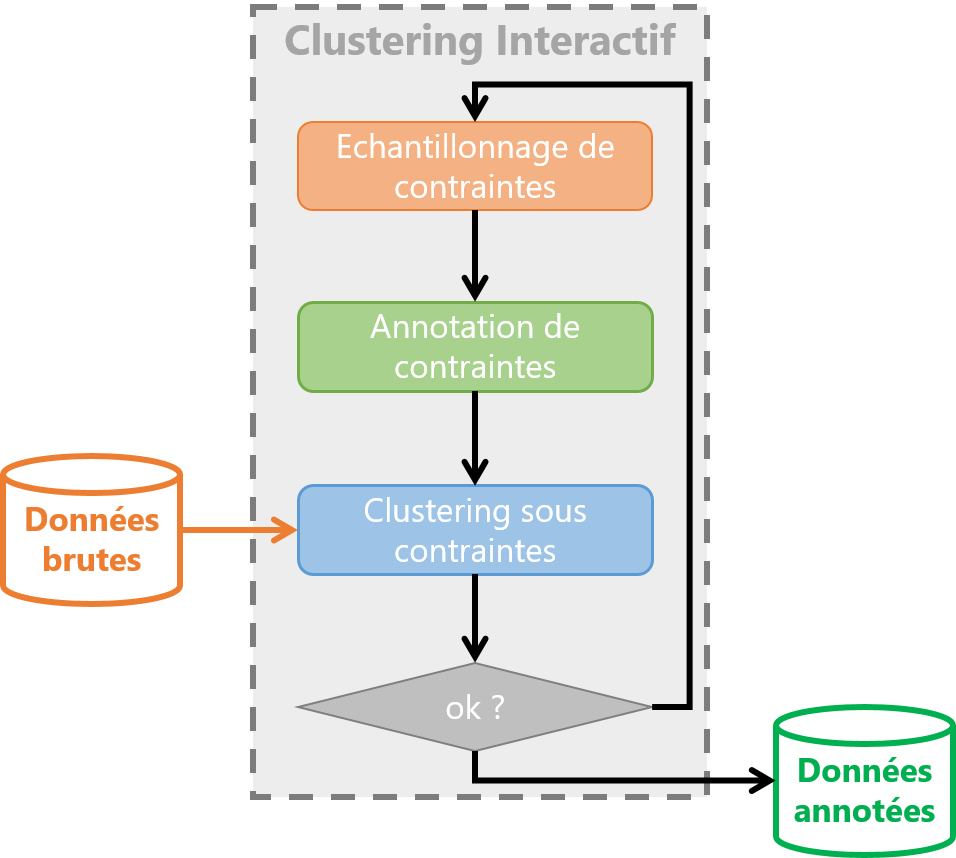
\includegraphics[width=0.95\textwidth]{figures/interactive-clustering-architecture-sequentielle}
			\caption{
				Schéma illustrant l'architecture du \textit{clustering} interactif.
				La boucle principale enchaîne un échantillonnage de couples de données, une annotation de contraintes, et un \textit{clustering} sous contraintes.
			}
			\label{figure:3.2-CLUSTERING-INTERACTIF}
		\end{figure}
	
	
	%%%
	%%% Subsection 3.2.2. Description détaillée.
	%%%
	\subsection{Description détaillée}
	\label{section:3.2.2-DESCRIPTION-THEORIQUE-DETAILLEE}
	
		% Pseudo code.
		L'\textsc{Algorithme~\ref{algorithm:3.2-CLUSTERING-INTERACTIF}} décrit formellement notre proposition de \texttt{Clustering Interactif} que nous détaillons ci-dessous.
		\begin{algorithm}
			\KwData{données non segmentées}
			\KwIn{budget à disposition}
			%
			\textbf{initialisation}: créer une liste vide de contraintes \;
			\textit{optionnel}: évaluer les hyper-paramètres de la segmentation automatique \;
			\textbf{segmentation initial}: regrouper les données par similarité \;
			\Repeat{segmentation satisfaisante OU budget épuisé}{
				\textit{optionnel}: évaluer les hyper-paramètres de l'échantillonnage \;
				\textbf{échantillonnage}: sélectionner une partie de la segmentation à corriger \;
				\textbf{annotation}: corriger la segmentation en ajoutant des contraintes sur l'échantillon \;
				\textit{optionnel}: ré-évaluer les hyper-paramètres de la segmentation automatique \;
				\textbf{segmentation}: regrouper les données par similarité avec les contraintes \;
				\textbf{validation}: estimer la pertinence et la stabilité de la segmentation \;
				\textbf{coûts}: estimer le budget restant et les coûts restant à investir \;
			}
			\textbf{interprétation}: trier et nommer les clusters pour les exploiter \;
			%
			\KwResult{données segmentées (i.e. base d'apprentissage)}
			%
			\caption{\textit{
				Description en pseudo-code de la méthode d'annotation proposée employant le \textit{clustering} interactif.
			}}
			\label{algorithm:3.2-CLUSTERING-INTERACTIF}
		\end{algorithm}
		
		% Description de l'initialisation.
		Pour l'\textbf{initialisation} de la méthode (cf. \textsc{Algorithme~\ref{algorithm:3.2-CLUSTERING-INTERACTIF}}, \textit{lignes 1 à 3}), nous définissons une liste vide de contraintes : tout au long du processus, nous y ajoutons les contraintes annotées par l'expert grâce à ses connaissances métiers (nous entrerons en détails en décrivant la phase d'annotation).
		Il faut aussi une première segmentation des données par la machine : celle-ci se réalise par l'exécution d'un algorithme de \textit{clustering}.
		Nous estimons qu'il n'est pas du ressort de l'expert métier de choisir le réglage de l'algorithme de \textit{clustering} et ses hyper-paramètres.
		Ces derniers pourront être déterminés par un \textit{data scientist} en fonction du problème à traiter ou laissés par défaut.
		Il est à noter que cette première segmentation des données est réalisée sans bénéficier de la connaissance de l'expert, il est donc peu probable que le résultat soit pertinent à ce stade.
		
		% Description de l'échantillonnage.
		Nous entrons dans le coeur de la boucle itérative par la phase d'\textbf{échantillonnage} (cf. \textsc{Algorithme~\ref{algorithm:3.2-CLUSTERING-INTERACTIF}}, \textit{lignes 5 et 6}).
		Comme mentionné au préalable, savoir quelles contraintes ajouter pour corriger efficacement le \textit{clustering} est un problème NP-difficile (le nombre de possibilités croît proportionnellement au carré du nombre de données).
		De plus, l'intervention d'experts est chiffrée et représente en général une partie des coûts à investir dans un projet (voir \textsc{Section~\ref{section:2.3.2.C-DEFIS-ANNOTATION-ASPECT-COMPLEXITE-COUTS}}).
		Il est donc inconcevable de laisser un expert métier annoter des contraintes "seul" et "au hasard".
		Ainsi, pour optimiser ses interventions, il convient de déterminer là où l'expert aura le plus d'impact lors de sa transmission de connaissances.
		C'est pourquoi la phase d'échantillonnage est primordiale dans la méthode proposée : Nous proposons d'y sélectionner des couples de données sur la base de leur similarité, de leur segmentation ou encore de leurs relations avec d'autres données déjà liées par des contraintes.
		
		% Description de l'annotation.
		Sur la base de cet échantillon, l'expert peut entamer son étape d'\textbf{annotation de contraintes} (cf. \textsc{Algorithme~\ref{algorithm:3.2-CLUSTERING-INTERACTIF}}, \textit{ligne 7}).
		Pour alléger la charge d'annotation, nous avons décidé de discriminer les données de l'échantillon par des contraintes binaires simples : \texttt{MUST-LINK} et \texttt{CANNOT-LINK}.
		Ces contraintes représentent respectivement la similitude ou la différence entre deux données, et seront utilisées pour regrouper ou séparer certaines données dans la prochaine segmentation.
		En fonction de l'orientation du projet et afin de rester au plus proche des compétences réelles de l'expert, la formulation de l'énoncer d'annotation doit être judicieusement définie : par exemple, les contraintes peuvent représenter une similitude
		sur la thématique concernée \footnote{
			Exemples de thématiques : \textit{crédit} vs. \textit{assurance} ; \textit{sport} vs. \textit{culture}, ...
		}, sur l'action désirée \footnote{
			Exemples d'actions : \textit{souscrire} vs. \textit{résilier} ; \textit{activer} vs. \textit{désactiver} ; \textit{s'informer} vs. \textit{réaliser}, ...
		}, ou encore sur le besoin de l'utilisateur \footnote{
			Exemple de besoins : \textit{souscrire un crédit} vs. \textit{souscrire une assurance} ; \textit{s'informer en sport} vs. \textit{s'informer en culture}, ...
		}.
		On notera que des incohérences peuvent s'introduire, ayant pour conclusions de devoir à la fois considérer comme similaires et différentes deux données : ces incohérences peuvent être détecter grâce à aux propriétés de transitivités des contraintes (voir la gestion des conflits en \textsc{Annexe~\ref{section:C.1.2-DESCRIPTION-IMPLEMENTATION-INTERACTIVE-CLUSTERING-GESTION-DES-CONTRAINTES}}).
		
		% Description du clustering.
		Pour finir, la dernière phase de cette boucle est composée d'une nouvelle \textbf{segmentation} des données (cf. \textsc{Algorithme~\ref{algorithm:3.2-CLUSTERING-INTERACTIF}}, \textit{lignes 8 et 9}).
		Cette segmentation devra respecter les contraintes préalablement définies par l'expert, nous nous tournons donc vers l'utilisation d'un \textit{clustering} sous contraintes.
		Au fur et à mesure des itérations, de plus en plus de contraintes seront ajoutées pour corriger le \textit{clustering}. ainsi, au bout d'un certain nombre d'itérations, la segmentation des données reflétera la vision que l'expert aura voulu transmettre.
		Comme précédemment, nous estimons qu'il n'est pas du ressort de l'expert métier de choisir de l'algorithme de \textit{clustering} et ses hyper-paramètres.
		Ces derniers pourront être déterminés par un \textit{data scientist} en fonction du problème à traiter, estimés en fonction de l'itération et des contraintes disponibles, ou laissés par défaut.
		
		% Description de l'évaluation.
		Comme la méthode est itérative, il faut pouvoir estimer des \textbf{cas d'arrêt} (cf. \textsc{Algorithme~\ref{algorithm:3.2-CLUSTERING-INTERACTIF}}, \textit{lignes 10 à 12}).
		Le cas d'arrêt le plus évident n'est pas technique mais relatif aux coûts investis dans l'opération : si le projet n'a plus de budget dédié à l'annotation, il faudra créer la base d'apprentissage avec le résultat à disposition, quel que soit la pertinence de la segmentation obtenue sur les données.
		Ce cas d'arrêt par défaut peut malheureusement être synonyme d'échec pour le projet si les résultats sont inexploitables.
		D'autres cas d'arrêts peuvent être envisagés en fonction de la qualité ou de la pertinence de la segmentation.
		D'une part, nous pouvons comparer l'évolution de la segmentation des données : si les segmentations sont similaires sur plusieurs itérations, il est possible que la modélisation atteint un optimum local ou un palier de performance.
		D'autre part, nous pouvons aussi comparer l'évolution de l'accord entre la segmentation obtenue et l'annotation de l'expert : en effet, si l'expert ne contredit plus la répartition proposée des données, il est probable que sa vision et la vision de la machine aient convergé.
		Dans les deux cas, l'analyse de l'expert métier reste nécessaire pour valider si la modélisation des données est pertinente ou si elle comporte encore des incohérences à corriger.

		% Description de l'évaluation.
		Lorsque la boucle itérative est finie, nous avons à disposition une segmentation des données qui a été corrigé par un expert et qui reflète ses connaissances métier.
		La dernière étape consiste alors à \textbf{interpréter} ces \textit{clusters} pour pouvoir les exploiter (cf. \textsc{Algorithme~\ref{algorithm:3.2-CLUSTERING-INTERACTIF}}, \textit{ligne 13}).
		Cela commence par leur attribuer un nom au lieu de leur identifiant technique, de les définir en les rapprochant d'un cas d'usage métier, et éventuellement de les raffiner manuellement en supprimant certaines données aberrantes.
		
		% Exemple abstrait.
		\begin{leftBarExamples}
			La \textsc{Figure~\ref{3.2-CLUSTERING-INTERACTIF-EXEMPLE}} déroule l'initialisation et la première itération de la méthode sur un exemple fictif.
			Nous pouvons constater qu'entre les images \textbf{(2)} et \textbf{(5)}, la segmentation des données à évoluée grâce à l'introduction de contraintes.
		
			\begin{figure}[H]
				\centering
				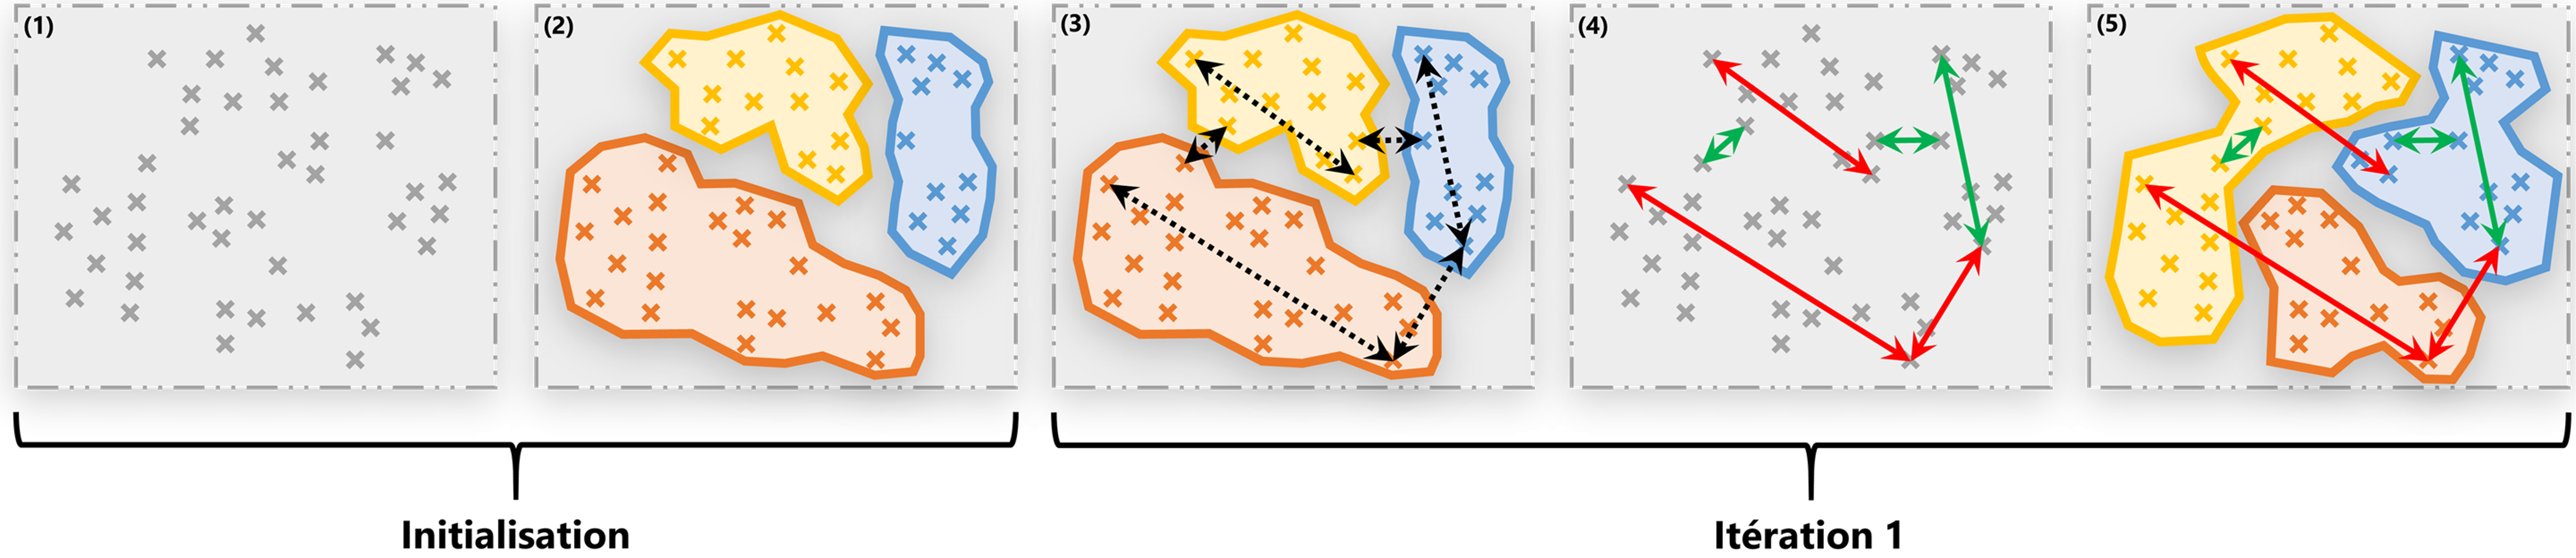
\includegraphics[width=0.95\textwidth]{figures/example-iteration-clustering-interatif}
				\caption{
					Exemple d'une itération de \textit{clustering} interactif. \\
					Lors de l'initialisation,
					\textbf{(1)} correspond au jeu de données brut,
					et \textbf{(2)} correspond à une première segmentation des données en $3$ \textit{clusters}.
					Lors de l'itération $1$ :
					\textbf{(3)} correspond à un exemple d'échantillonnage de $6$ contraintes représentées par les flèches en pointillées,
					\textbf{(4)} correspond à la caractérisation de ces $6$ contraintes par des liens \texttt{MUST-LINK} en vert et \texttt{CANNOT-LINK} en rouge,
					et \textbf{(5)} correspond à la nouvelle segmentation des données en $3$ \textit{clusters} respectant les $6$ contraintes annotées.
					La prochaine itération se poursuivra par un nouvel échantillonnage de contraintes.
				}
				\label{3.2-CLUSTERING-INTERACTIF-EXEMPLE}
			\end{figure}
		\end{leftBarExamples}
	

	
	%%%
	%%% Subsection 3.2.3. Description techniques et implémentation.
	%%%
	\subsection{Description techniques et implémentation}
	\label{section:3.2.3-DESCRIPTION-TECHNIQUE-IMPLEMENTATION}
	
		% Généralités.
		Au cours de ce doctorat, nous avons réalisé une implémentation en Python de notre \textit{clustering interactif}.
		Celle-ci est répartie en trois librairies :
		\begin{enumerate}
			% cognitivefactory-interactive-clustering
			\item \texttt{cognitivefactory-interactive-clustering} \footnote{
				\texttt{cognitivefactory-interactive-clustering}: la page de documentation technique de cette librairie est disponible ici : \url{https://cognitivefactory.github.io/interactive-clustering/}
			} (\cite{schild:2022:cognitivefactory-interactiveclustering}), regroupant les gestions de données, la gestion des contraintes, les algorithmes de \textit{clustering} sous contraintes et les algorithmes d'échantillonnage implémentés ;
			% cognitivefactory-features-maximization-metric
			\item \texttt{cognitivefactory-features-maximization-metric} \footnote{
				\texttt{cognitivefactory-features-maximization-metric}: la page de documentation technique de cette librairie  est disponible ici : \url{https://cognitivefactory.github.io/features-maximization-metric/}
			} (\cite{schild:2023:cognitivefactory-featuresmaximizationmetric}), disposant d'une méthode de sélection des patterns linguistiques pertinents (composantes principales) d'un jeu de données, utilisée pour l'analyse de pertinence d'un résultat de \textit{clustering} ;
			% cognitivefactory-interactive-clustering-gui
			\item \texttt{cognitivefactory-interactive-clustering-gui} \footnote{
				\texttt{cognitivefactory-interactive-clustering-gui}: la page de documentation technique de cette librairie  est disponible ici : \url{https://cognitivefactory.github.io/interactive-clustering-gui/}
			} (\cite{schild-etal:2022:cognitivefactory-interactiveclusteringgui}), encapsulant les algorithmes précédents et intégrant la logique de la méthode dans une application web.
		\end{enumerate}
		
		


	%%%%%--------------------------------------------------------------------
	%%%%% Section 3.3: Perspectives portés sur la méthode proposée.
	%%%%%--------------------------------------------------------------------
	%\newpage
	%\vspace{2cm}
	\section{Perspectives portées par la méthode proposée.}
\label{section:3.3-PERSPECTIVES-METHODE}

	% Rappel de la proposition.
	Nous avons proposé une méthodologie d'annotation basée sur une interaction entre l'Homme et la Machine dans le but de soulager l'expert métier dans son intervention.
	
	% Annonce des perspectives.
	Grâce à une telle approche, nous pouvons espérer que :
	\begin{todolist}
		\item Les experts métiers n'auront désormais plus besoin de bagages analytiques ou techniques pour intervenir dans un projet d'annotation ;
		\item Les experts métiers pourront désormais participer à la modélisation d'une base d'apprentissage en ayant des discussions pragmatiques sur les cas d'usages des données manipulées ;
		\item Une telle méthodologie d'annotation permettra d'obtenir efficacement une base d'apprentissage stable et pertinente pour entraîner une modèle de classification d'intention ;
		\item Une telle méthodologie d'annotation sera réaliste en terme de délais et d'investissement financier.
	\end{todolist}
	
	% Transition au chapitre 4.
	Nous allons explorer diverses pistes pour confirmer ou infirmer ces perspectives dans le \textsc{Chapitre~\ref{chapter:4-ETUDES}}, et nous détaillerons nos conclusions dans un guide d'utilisation qui sera présenté dans le \textsc{Chapitre~\ref{chapter:5-GUIDE}}.

%%%%%--------------------------------------------------------------------
%%%%% Chapitre: Etude de la méthode
%%%%%--------------------------------------------------------------------
\chapter{Étude de six hypothèses sur le \textit{Clustering Interactif}}
\label{chapter:4-ETUDES}
	
	% RÉSUMÉ DES ÉPISODES PRÉCÉDENTES:
	Dans le chapitre précédent, nous avons présenté une méthode de création d'un jeu de données d'entraînement pour un assistant conversationnel, que nous appelons "\textit{clustering interactif}" :
	%
	\begin{leftBarImportantGreen}
		\begin{todolist}
			% 1. Structure de la méthode.
			\item[\itemok] La méthode proposée repose sur la combinaison entre un regroupement automatique des données par la machine et l'annotation de contraintes binaires par un expert métier pour corriger le regroupement proposé ;
			% 2. Enjeu 1 de la méthode : moins de technique.
			\item[\itemok] Une telle approche devrait limiter les pré-requis techniques actuellement exigés à un expert métier en les déléguant à la machine.
			% 2. Enjeu 2 de la méthode : plus de connaissance métier.
			\item[\itemok] En échange, l'expert se concentre d'avantage sur la transmission de ses connaissances avec une annotation caractérisant la similitude métier entre deux données.
			% 3. Divers.
			\item[\itemok] ...
		\end{todolist}
	\end{leftBarImportantGreen}
	\todo[inline]{divers à compléter (technique ? méthode ? ...).}
	
	% ANNONCE DU BUT DU CHAPITRE: TEST DE LA MÉTHODE.
	Comme nous l'avons détaillé dans le \textsc{Chapitre~\ref{chapter:2-REVUE-DE-LITTERATURE}}\todo{a revoir}, des procédés d'annotation similaires existent pour des données facilement visualisables, comme dans le cadre du traitement d'images.
	Cependant, l'application d'une telle approche dans le cadre de la classification de données textuelles est peu détaillée dans la littérature.
	Ainsi, dans cette partie, nous étudions la faisabilité d'un tel \textit{clustering interactif} pour des données textuelles en explorant les questions suivantes :
	%
	\begin{leftBarImportantRed}
		\begin{todolist}
			% 1. Efficacité.
			\item Peut-on obtenir une base d'apprentissage à l'aide de notre proposition d'implémentation de la méthodologie du \textit{clustering} interactif ? (cf. hypothèse d'\textbf{efficacité} en \textsc{Section~\ref{section:4.1-HYPOTHESE-EFFICACITE}}) ;
			% 2. Efficience.
			\item Peut-on déterminer un paramétrage optimal de cette implémentation pour obtenir plus rapidement une base d'apprentissage ? (cf. hypothèse d'\textbf{efficience} en \textsc{Section~\ref{section:4.2-HYPOTHESE-EFFICIENCE}}) ;
			% 3. Coûts.
			\item D'après les données initiales, peut-on approximer l'investissement nécessaire pour obtenir une base d'apprentissage exploitable ? (cf. hypothèse sur les \textbf{coûts} en \textsc{Section~\ref{section:4.3-HYPOTHESE-COUTS}}) ;
			% 4. Pertinence.
			\item A un instant donné, peut-on estimer la pertinence métier d'une base d'apprentissage en cours de construction ? (cf. hypothèse de \textbf{pertinence} en \textsc{Section~\ref{section:4.4-HYPOTHESE-PERTINENCE}}) ;
			% 5. Impact.
			\item Au cours du processus de construction de la base d'apprentissage, peut-on aisément estimer les potentiels d'une étape de raffinage supplémentaire ? (cf. hypothèse de \textbf{rentabilité} en \textsc{Section~\ref{section:4.5-HYPOTHESE-RENTABILITE}}) ;
			% 6. Robustesse.
			\item Peut-on estimer l'influence d'une différence d'annotation dans la construction de la base d'apprentissage ? (cf. hypothèse de \textbf{robustesse} en \textsc{Section~\ref{section:4.6-HYPOTHESE-ROBUSTESSE}}).
		\end{todolist}
	\end{leftBarImportantRed}
	
	% ILLUSTRATION: SCHEMA DES HYPOTHESES
	Afin d'illustrer ces interrogations, nous vous proposons de considérer de la \textsc{Figure~\ref{figure:4.0-HYPOTHESE-00-DEFAULT}}. Dans les sections suivantes, cette figure évoluera pour résumer les études réalisées.
	%
	\begin{figure}[!htb]
		\centering
		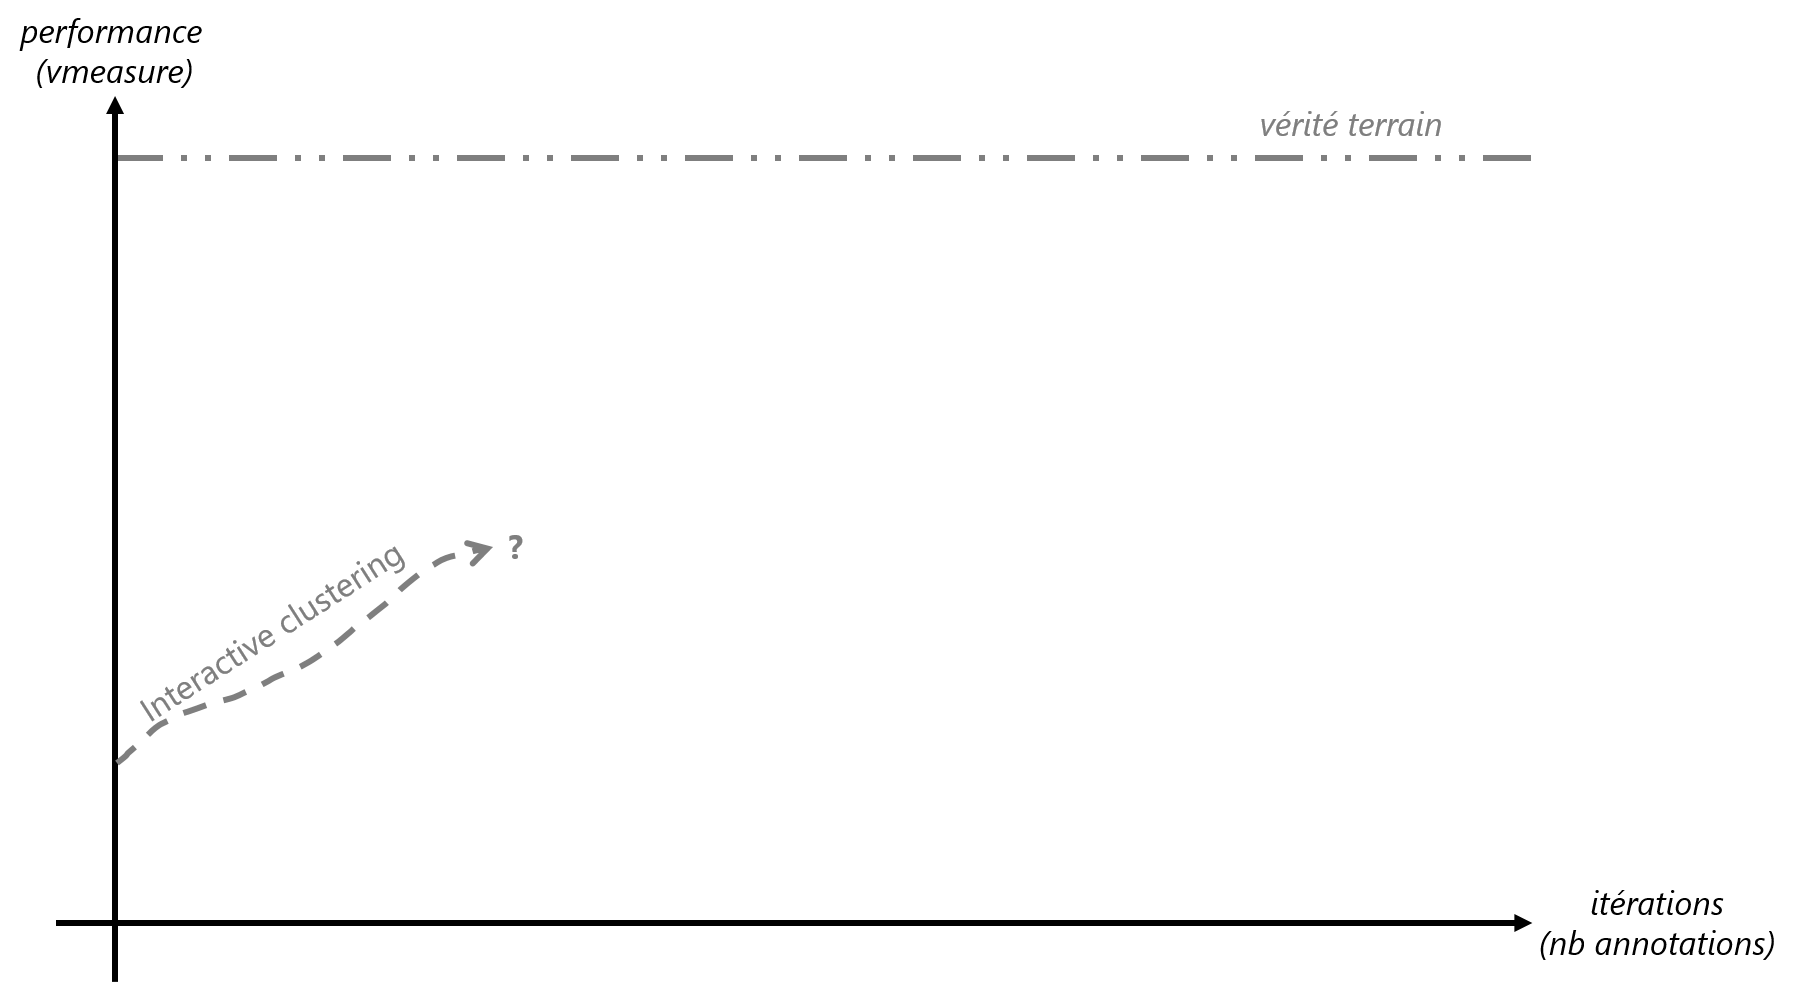
\includegraphics[width=0.95\textwidth]{figures/hypotheses-00-default}
		\caption{
			Illustration des études réalisées sur le \textit{clustering} interactif (\textit{étape 0/6}) en schématisant l'évolution de la performance (\textit{accord avec la vérité terrain calculé en v-measure}) d'une base d'apprentissage en cours de construction en fonction du nombre d'itérations de la méthode (\textit{nombre d'annotations par un expert métier}).
		}
		\label{figure:4.0-HYPOTHESE-00-DEFAULT}
	\end{figure}
	
	\todo[inline]{
		Pour ces études, nous allons (1) faire des analyses théoriques (2) des analyses empiriques (car dans la vrai vie on n'a pas de vérité terrain).
		Nous utilisons aussi la vmeasure.
	}
	\todo[inline]{
		Table des nomenclatures.
	}
	
	% PRÉAMBULE TECHNIQUE : CPU + scrips + datasets.
	\begin{leftBarInformation}
		Pour ces études, l'exécution des différentes expériences a été réalisée sur des CPU \texttt{Intel(R) Xeon(R) CPU E5-2660 v4 \@ 2.00GHz} et parallélisé avec la librairie Python \textit{multiprocessing} (un worker par CPU).
		Les scripts d'exécution et d'analyse de ces expériences, rédigés au sein de \textit{notebooks} Python (\cite{van-rossum-drake:2009:python-reference-manual}) ou de script R (\cite{r-core-team:2017:language-environment-statistical}), sont disponibles dans \cite{schild:2021:cognitivefactory-interactiveclusteringcomparativestudy}.
		Enfin, les jeux de données utilisés pour ces études sont détaillés en Annexe~\ref{annex:A-ANNEXE-DATASET}.
	\end{leftBarInformation}
	
	
	% TABLE DES MATIÈRES DU CHAPITRE
	\minitoc
	
	%%%%%--------------------------------------------------------------------
	%%%%% Section 4.1: Hypothèse d'efficacité.
	%%%%%--------------------------------------------------------------------
	\newpage
	\section{Évaluation de l'hypothèse d'efficacité}
\label{section:4.1-HYPOTHESE-EFFICACITE}
%  : « \textit{est-ce que la méthode permet d'annoter un jeu de données ?} »
	
	%%% Formulation des hypothèses:
	Nous aimerions vérifier l'hypothèse suivante :

	\begin{tcolorbox}[
		title=\faVial~\textbf{Hypothèse d'efficacité}~\faVial,
		colback=colorTcolorboxHypothesis!15,
		colframe=colorTcolorboxHypothesis!75,
		width=\linewidth
	]
		% Hypothèse.
		« \textbf{
			Une méthodologie d'annotation basée sur le \textit{clustering} interactif permet d'obtenir une base d'apprentissage pour un assistant conversationnel qui respecte la vision donnée par l'expert métier au cours de l'annotation.
		} » \\
		
		% Résumé de l'étude.
		Afin de vérifier cette hypothèse, nous mettrons en place une expérience de ré-annotation d'une base d'apprentissage (qui servira ici de vérité terrain) à l'aide de notre méthode, en simulant l'annotation d'un expert, et nous critiquerons l'évolution de la nouvelle base d'apprentissage obtenue et sa similitude avec la base d'apprentissage initiale.
		
		% Figure.
		La figure~\ref{figure:4.1-HYPOTHESE-EFFICACITE} illustre cette hypothèse et l'espoir de convergence d'une base d'apprentissage en cours de construction vers sa vérité terrain.
		%
		\begin{figure}[H]  % keep [H] to be in the tcolorbox.
			\centering
			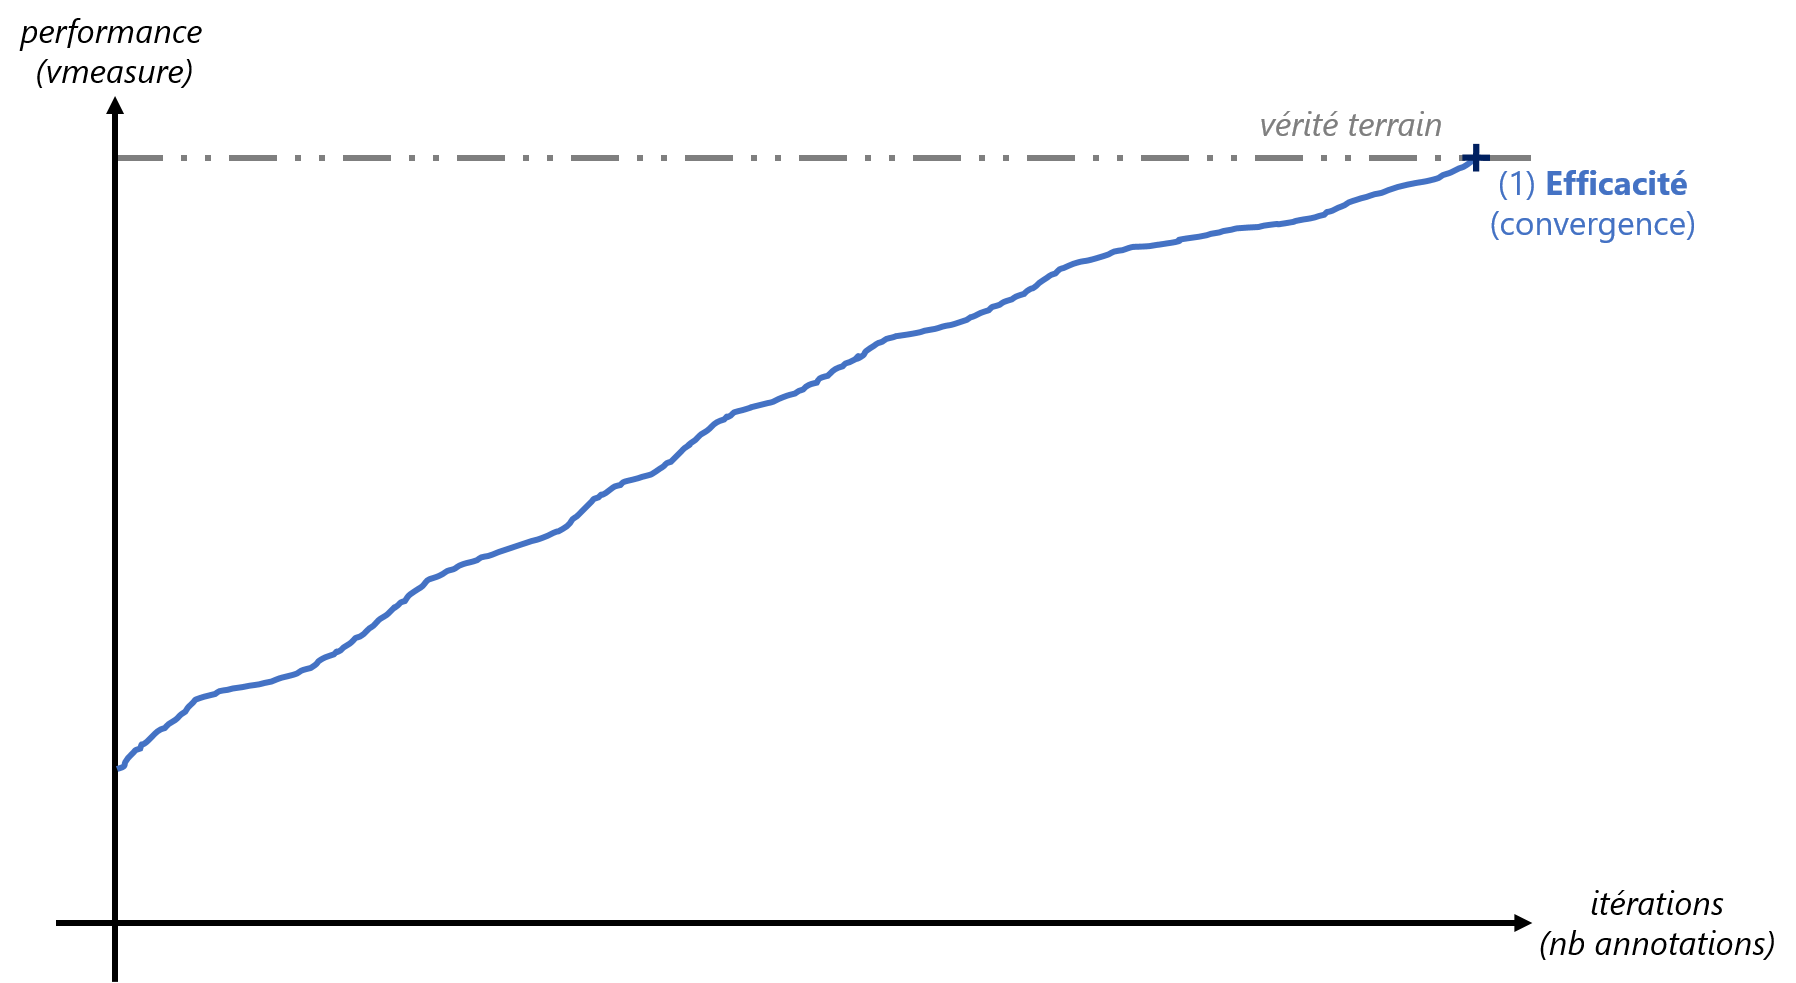
\includegraphics[width=0.8\textwidth]{figures/hypotheses-01-efficacite}
			\caption{Illustration des études réalisées sur le \textit{clustering} interactif (\textit{étape 1/6}) en schématisant l'évolution de la performance (\textit{accord avec la vérité terrain calculé en v-measure}) d'une base d'apprentissage en cours de construction en fonction du nombre d'itérations de la méthode (\textit{nombre d'annotations par un expert métier}).}
			\label{figure:4.1-HYPOTHESE-EFFICACITE}
		\end{figure}

	\end{tcolorbox}
	
	%%%
	%%% Subsection 4.1.1: Étude de convergence
	%%%
	\subsection{Étude de convergence vers une vérité terrain pré-établie}
	\label{subsection:4.1.1-ETUDE-CONVERGENCE}
			
		% Référence articles.
		\begin{leftBarInformation}
			Cette étude a été l'objet d'une présentation à la conférence \texttt{EGC (Extraction et Gestion des Connaissances)}~\citep{schild:conception-interactive-clustering:2021}, et d'une extension dans le journal \texttt{IJDWM (International Journal of Data Warehousing and Mining)}~\citep{schild:extension-interactive-clustering:2022}.
			\footnote{Les résultats et la discussion ont été mis à jour et réécrits pour mieux s'intégrer au discours ce manuscrit.}
		\end{leftBarInformation}

		%%% Protocole expérimental.
		\subsubsection{Protocole expérimental : simuler l'annotation d'une base d'apprentissage}
		
			% Objectif de l'expérience.
			Nous voulons vérifier qu'une méthodologie d'annotation basée sur notre implémentation du \textit{clustering} interactif permet de créer une base d'apprentissage pour un assistant conversationnel.
			Pour cela, nous prenons une base d'apprentissage employée pour entraîner un modèle de classification de textes\todo{référence, lien vers ANNEXE, + description conditions de création du JDD}, et nous utilisons ce jeu de données comme vérité terrain.
			L'objectif de cette expérience est de simuler la création de cette base d'apprentissage et de nous assurer que le résultat obtenu correspond à la vérité terrain.
			
			% Axiome.
			\begin{leftBarWarning}
				Dans le cadre de cette étude, nous supposons que l'expert métier connaît parfaitement le domaine traité dans ce jeu de données, et qu'il est capable de caractériser sans ambiguïté la similitude entre deux données issues de cet ensemble.
			\end{leftBarWarning}
			
			% Détails de l'expérience.
			Lors de cette expérience, chaque tentative de la méthode commencera sur la version non labellisée de la vérité terrain à disposition, sans aucune contrainte connue à l'avance.
			Au fur et à mesure des itérations de la méthode, nous simulerons l'annotation de l'expert métier en comparant les labels de la vérité terrain : ainsi, deux données ont une contrainte \texttt{MUST-LINK} si elles ont le même label, et une contrainte \texttt{CANNOT-LINK} sinon. Cela traduit le prérequis d'avoir un annotateur qui soit capable, dans son domaine d'expertise,  de différencier deux données selon leur ressemblance.
			Une tentative de l'application de notre méthode s'arrête lorsque toutes les contraintes possibles entre les données ont été annotés par l'expert.

			% Description implémentation de l'interactive clustering.
			Pour cette étude, nous essayons une tentative pour chaque combinaison de paramètre de notre implémentation du clustering interactif (cf. section~\ref{section:3.3-DESCRIPTION-IMPLEMENTATION}). Cela comprend les tâches et leurs paramètres respectifs suivants :
			%
			\begin{enumerate}
				\item le \textbf{prétraitement} des données, avec les niveaux suivants : \textbf{absent} (\texttt{prep.no}), \textbf{simple} (\texttt{prep.simple}), \textbf{avec lemmatisation} (\texttt{prep.lemma}) et \textbf{avec filtres} (\texttt{prep.filter}) ;
				\item la \textbf{vectorisation} des données, avec les niveaux suivants : \textbf{TF-IDF} (\texttt{vect.tfidf}) et \textbf{SpaCy} (\texttt{vect.frcorenewsmd}) ;
				\item le \textbf{clustering sous contraintes} des données, avec les niveaux suivants : \textbf{KMeans} (modèle \textit{COP} : \texttt{clust.kmeans.cop}), \textbf{Hiérarchique} (lien \textit{single}: \texttt{clust.hier.sing} ; lien \textit{complete} \texttt{clust.hier.comp} ; lien \textit{average} : \texttt{clust.hier.avg} ; lien \textit{ward} : \texttt{clust.hier.ward}) et \textbf{Spectral} (modèle \textit{SPEC} : \texttt{clust.spec}). Le choix du nombre de clusters n'est pas étudié ici, et ce nombre est fixé au nombre de classes présentes dans la vérité terrain ;
				\item l'\textbf{échantillonnage} des contraintes à annoter, avec les niveaux suivants : \textbf{purement aléatoire} (\texttt{samp.random.full}), \textbf{pseudo-aléatoire} (\texttt{samp.random.same}), \textbf{même cluster et étant les plus éloignées} (\texttt{samp.farhtest.same}) et \textbf{clusters différents et étant les plus proches} (\texttt{samp.closest.diff}). La choix de la taille d'échantillon n'est pas étudié ici, et cette taille est arbitrairement fixé à \texttt{50}.
			\end{enumerate}
			
			Il y a donc \texttt{192} combinaisons testées, et chaque tentative est répétée \texttt{5} fois pour contrer les aléas statistiques de certains algorithmes.
			Pour plus de détails sur ces algorithmes, référez-vous à la section~\ref{section:3.3-DESCRIPTION-IMPLEMENTATION} pour avoir accès à leur description, à leurs paramètres et aux choix d'implémentation.
			
			% Description de l'évaluation.
			Pour évaluer l'équivalence entre la vérité terrain et notre segmentation des données obtenue au cours de la méthode, nous nous intéresserons à l'évolution de la \texttt{v-measure} entre ces deux jeu de données.
			Si le score du calcul de la \texttt{v-measure} est de \texttt{100\%}, cela signifierait que le clustering final et la vérité terrain propose une segmentation identique des données, donc que la vérité terrain a pu être retrouvée, et donc qu'il est possible d'obtenir une base d'apprentissage pour un assistant conversationnel à l'aide d'une méthodologie d'annotation basée sur le \textit{clustering} interactif.
			
			% Pseudo-code.
			Pour résumer ce protocole expérimental, vous pouvez vous référez au pseudo-code décrit dans Alg.~\ref{algorithm:4.1.1-ETUDE-CONVERGENCE-PROTOCOLE}.
			%
			\begin{algorithm}[!htb]
				\begin{algorithmic}[1]
					\Require jeu de données annoté (vérité terrain)
					\ForAll{arrangement d'algorithmes et de paramètres à tester}
						\State \textbf{initialisation}: récupérer les données de la vérité terrain sans leur label, créer une liste vide de contraintes
						\State \textbf{prétraitement}: supprimer le bruit dans les données
						\State \textbf{vectorisation}: transformer les données en vecteurs
						\State \textbf{clustering initial}: regrouper les données par similarité
						\State \textbf{évaluation}: estimer l'équivalence entre le clustering obtenu et la vérité terrain
						\Repeat
							\State \textbf{échantillonnage}: sélectionner de nouvelles contraintes à annoter
							\State \textbf{simulation d'annotation}: ajouter des contraintes grâce à la comparaison des labels de la vérité terrain
							\State \textbf{clustering}: regrouper les données par similarité avec les contraintes
							\State \textbf{évaluation}: estimer l'équivalence entre le clustering obtenu et la vérité terrain
						\Until{annotation de toutes les contraintes possibles}
						\State \textbf{évaluation finale}: espérer avoir un score d'équivalence de 100\% entre le clustering obtenu et la vérité terrain
					\EndFor
					\Ensure arrangements d'algorithmes et de paramètres ayant un score d'équivalence de 100\%
				\end{algorithmic}
				\caption{Description en pseudo-code du protocole expérimental de l'étude de convergence du \textit{clustering} interactif vers une vérité terrain pré-établie.}
				\label{algorithm:4.1.1-ETUDE-CONVERGENCE-PROTOCOLE}
			\end{algorithm}
			
			% Référence scripts.
			\begin{leftBarInformation}
				Les scripts de l'expérience (\textit{notebooks} Python) sont disponibles dans un dossier dédié de~\cite{schild:cognitivefactory-interactive-clustering-comparative-study:2021}.
			\end{leftBarInformation}

		%%% Résultats.
		\subsubsection{Résultats obtenus}
			
			% Graphe d'évolution de la v-measure moyenne, min et max.
			La figure~\ref{figure:4.1.1-ETUDE-CONVERGENCE-EVOLUTION} et le tableau~\ref{table:4.1.1-ETUDE-CONVERGENCE-EVOLUTION} représentent l'évolution moyenne de la \texttt{v-measure} du clustering en fonction du nombre d'itération de la méthode. Les tentatives les plus rapides et les plus lentes sont représentées sur la figure.
							
			% Tendance: Forte dispersion, Croissance générale.
			Malgré une forte dispersion des résultats (écart-type de \texttt{v-measure} pouvant être supérieur à 20\%, forte différence entre les tentatives la plus rapide et la plus lente) et quelques sauts de performances (cf. à-coups de la tentative la plus lente sur la figure), une convergence générale vers la vérité terrain peut être constatée.
			
			% Tendance à courts termes: Croissance linéaire
			A l'itération \texttt{0}, une tentative commence avec une moyenne de \texttt{19.05}\% de \texttt{v-measure}  entre son \textit{clustering} initial (sans contraintes) et la vérité terrain.
			Cette \texttt{v-measure} moyenne croît presque linéairement (pente de \texttt{0.97}) jusqu'à l'itération 75 où elle atteint la performance de \texttt{92.08}\% (cf. tableau~\ref{table:4.1.1-ETUDE-CONVERGENCE-EVOLUTION}).

			% Tendance à longs termes: Asymptote.
			Au delà de l'itération 75, la courbe de la \texttt{v-measure} moyenne tend vers une asymptote de {100}\% (cf. figure~\ref{figure:4.1.1-ETUDE-CONVERGENCE-EVOLUTION}).
			Cette asymptote est atteinte par toute les \texttt{960} tentatives (\texttt{192} combinaisons de paramètres, \texttt{5} tentatives pour chaque combinaison), la tentative l'ayant atteinte le plus tôt à l'itération 19 et celle le plus tard à l'itération 326.
			La courbe se prolonge jusqu'à l'itération \texttt{394} pour que toutes les tentatives puisse annoter toutes les contraintes possibles sur le jeu de données.
			
			%
			\begin{figure}[!htb]
				\centering
				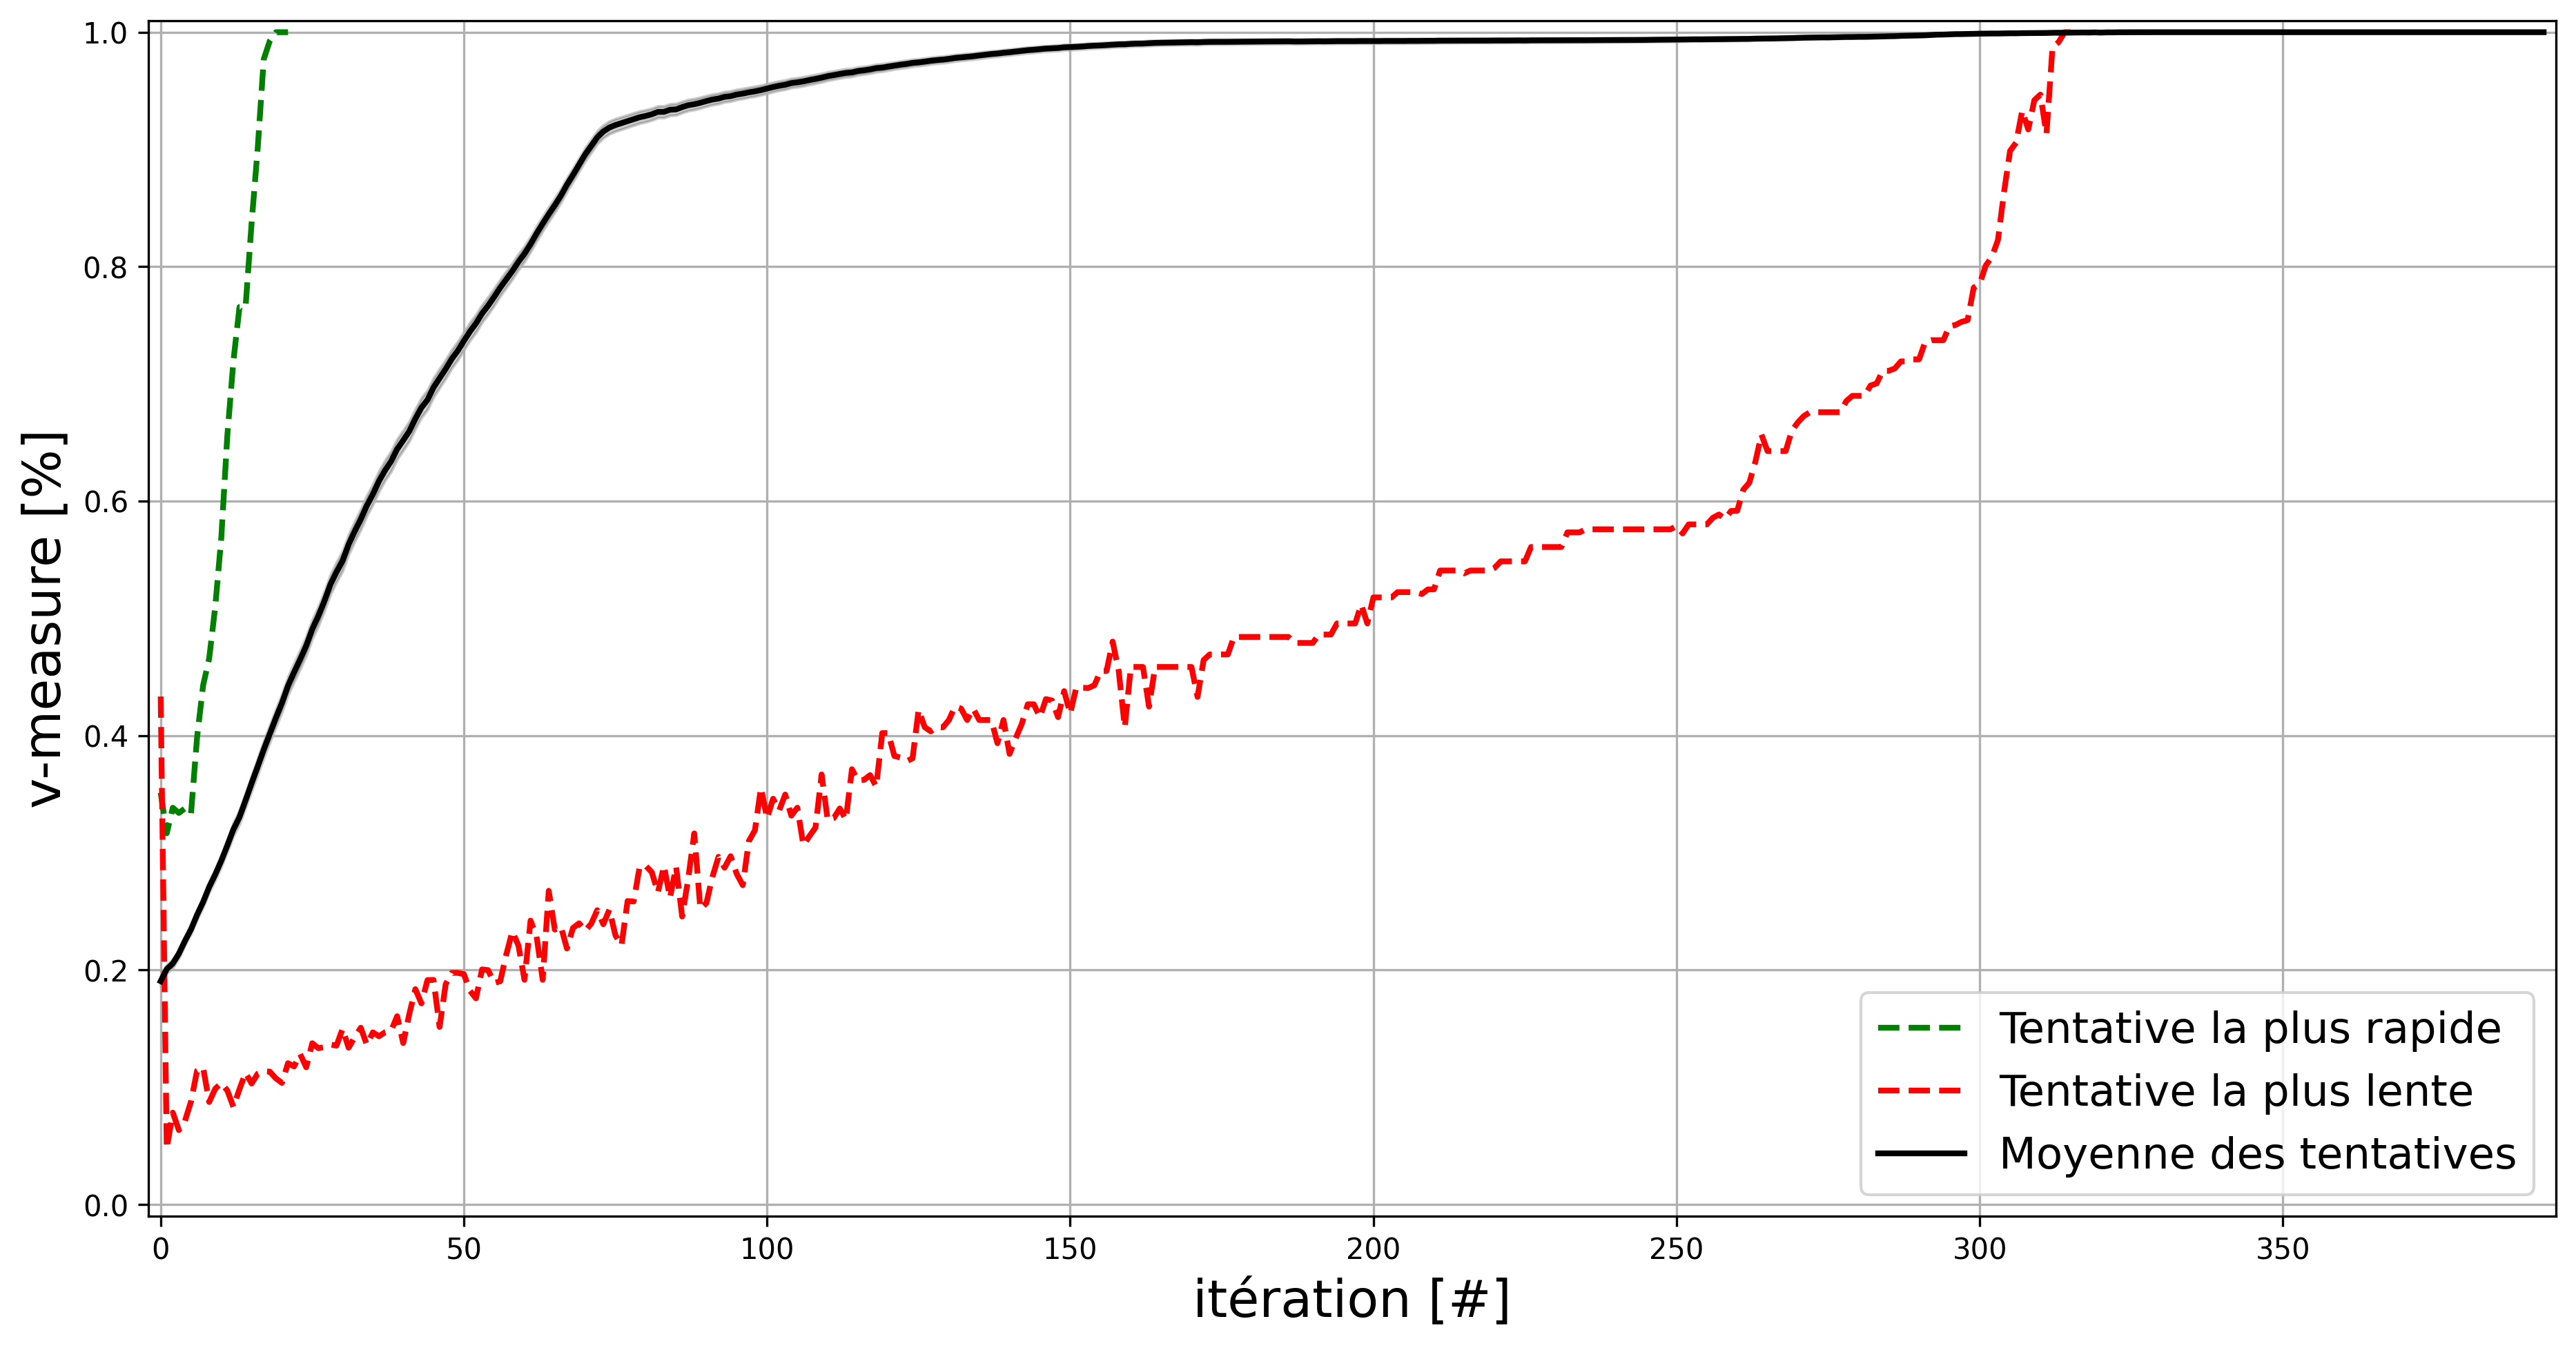
\includegraphics[width=0.8\textwidth]{figures/etude-efficacite-evolution-moyenne-0par-iteration}
				\caption{Évolution de la moyenne de la \texttt{v-measure} entre un résultat obtenu et la vérité terrain en fonction du nombre d'itération de la méthode de \textit{clustering} interactif, moyenne réalisée itération par itération sur l'ensemble des tentatives.
				Représentation des tentatives ayant été les plus rapides (\textit{un prétraitement \texttt{prep.simple}, une vectorisation \texttt{vect.tfidf}, un clustering \texttt{clust.hier.comp} ou \texttt{clust.hier.ward}, et un échantillonnage \texttt{samp.closest.diff}}) et les plus lentes (\textit{un prétraitement \texttt{prep.no}, une vectorisation \texttt{vect.tfidf}, un clustering \texttt{clust.spec}, et un échantillonnage de contraintes \texttt{samp.farthest.same}}) pour atteindre 100\% de \texttt{v-measure}.}
				\label{figure:4.1.1-ETUDE-CONVERGENCE-EVOLUTION}
			\end{figure}
			%
			\begin{table}[!htb]
				\begin{center}
				\begin{tabular}{|c|r|r|r|r|r|}
					\hline
					% ENTETE DU TABLEAU
					\multicolumn{2}{|c|}{ \shortstack{ Annotations } }
						& \multicolumn{4}{c|}{ \shortstack{ Performances (\texttt{v-measure}) } }
						\tabularnewline
						\hline
					\multicolumn{1}{|c|}{ \shortstack{ Itérations } }
						& \multicolumn{1}{c|}{ \shortstack{ Contraintes } }
						& \multicolumn{1}{c|}{ \shortstack{ Moyenne } }
						& \multicolumn{1}{c|}{ \shortstack{ Écart-type } }
						& \multicolumn{1}{c|}{ \shortstack{ Minimum } }
						& \multicolumn{1}{c|}{ \shortstack{ Maximum } }
						\tabularnewline
						\hline
					%
					0	& 0		& \( 19.05\% \) \footnotesize \( (\pm0.43) \) \par	& \( 13.38\% \) & \( 03.42\% \) & \( 47.75\% \)
					\tabularnewline
					\hline
					%
					25	& 1 250	& \( 49.09\% \) \footnotesize \( (\pm0.82) \) \par	& \( 25.43\% \) & \( 09.09\% \) & \( 100.00\% \)
					\tabularnewline
					\hline
					%
					50	& 2 500	& \( 73.66\% \) \footnotesize \( (\pm0.77) \)	 \par& \( 23.98\% \) & \( 16.78\% \) & \( 100.00\% \)
					\tabularnewline
					\hline
					%
					75	& 3 750	& \( 92.08\% \) \footnotesize \( (\pm0.54) \) \par	& \( 16.70\% \) & \( 21.74\% \) & \( 100.00\% \)
					\tabularnewline
					\hline
					%
					100	& 5 000	& \( 95.19\% \) \footnotesize \( (\pm0.41) \) \par	& \( 12.67\% \) & \( 26.93\% \) & \( 100.00\% \)
					\tabularnewline
					\hline
					%
					125	& 6 250	& \( 97.43\% \) \footnotesize \( (\pm0.29) \) \par	& \( 09.09\% \) & \( 34.99\% \) & \( 100.00\% \)
					\tabularnewline
					\hline
					%
					150	& 7 500	& \( 98.73\% \) \footnotesize \( (\pm0.23) \) \par	& \( 07.22\% \) & \( 38.14\% \) & \( 100.00\% \)
					\tabularnewline
					\hline
					
				\end{tabular}
				\end{center}
				\caption{Détails de l'évolution de la moyenne de la \texttt{v-measure} entre un résultat obtenu et la vérité terrain en fonction du nombre d'itération de la méthode de \textit{clustering} interactif, moyenne réalisée itération par itération sur l'ensemble des tentatives.}
				\label{table:4.1.1-ETUDE-CONVERGENCE-EVOLUTION}
			\end{table}

		%%% Discussion
		\subsubsection{Discussion}
			
			%%% Principale conclusion : il y a convergence !
			La première et principale conclusion de cette étude concerne la preuve que la méthode est efficace.
			En effet, les différentes simulations ont bien convergé vers la vérité terrain (atteinte de l'asymptote à \texttt{100}\% de \texttt{v-measure}), montrant qu'il est possible pour un expert métier de créer une base d'apprentissage à l'aide d'une méthodologie d'annotation basée sur le \textit{clustering} interactif. \\
			
			
			%%% Avantages.
			Cette découverte permet de confirmer plusieurs espoirs portés sur la méthode. 
			
			% Avantage 1 : Émergence d'une modélisation sur la base des contraintes
			Tout d'abord, la vérité terrain a été retrouvée sans formaliser concrètement la structure de données.
			Là où une annotation par label aurait requis au préalable une définition des catégories possibles pour les données à étiqueter, la méthodologie employant le \textit{clustering} interactif a permis de faire émerger naturellement cette structure de données.
			Cette émergence provient directement des contraintes annotées par l'expert métier, traduisant ainsi ses connaissances à l'aide d'instructions simples : \textit{les données sont-elles ou non similaires ?}
			
			% Avantage 2 : annotations plus simples et plus concrètes
			De plus, ces contraintes ont été l'objet d'une annotation guidée par les besoins de la machine afin de s'améliorer d'itération en itération (voir la croissance globale de la \texttt{v-measure} sur la figure~\ref{figure:4.1.1-ETUDE-CONVERGENCE-EVOLUTION}).
			Ainsi, l'expert métier corrige la base d'apprentissage à chaque itération : soit en affinant les clusters en cours de construction, améliorant ainsi la cohérence des clusters (cf. pentes croissantes) ; soit en remaniant les clusters mal formés pour repartir sur de bonnes bases, détériorant la cohérence des clusters le temps de la réorganisation (cf. oscillations ou pentes décroissantes). \\

			
			%%% Limites.
			Néanmoins, différentes pistes sont encore à explorer pour rendre le \textit{clustering} interactif utilisable en situation réelle.
			
			% Limite 1 : Nombre d'annotations ==> besoin d'optimisation.
			D'une part, nous échangeons le besoin de définir une structure de données contre la nécessité d'annoter un grand nombre de contraintes : pour \texttt{500} points de données, et en considérant que l'asymptote à \texttt{100}\% est atteinte en moyenne autour de l'itération \texttt{200}, il faudrait \texttt{10 000} annotations de contraintes pour être exhaustif, ce qui correspond à près de \texttt{20} fois plus de contraintes que de données.
			Bien que l'annotation binaire demande a priori une charge mentale plus faible à un annotateur, un tel volume représente tout de même une grande quantité de travail.
			\todo{
				Commentaire Gautier 22/05/2023 :
				(A DÉTAILLER AILLEURS ?)
				Oui, complètement d'accord ici, mais en fait ça va plus loin que ça non ?
				Déjà, on a une quantité de ressources allouées à la tâche en effet plus fabile (car choisir entre "similaire" et "non similaire" est clairement plus simple que d'assigner un label parmi N).
				Mais on a aussi une diminution des ressources allouées au maintien d'une stratégie d'annotation : en effet, pas besoin de définir à l'avance de type system ou autre, tout est construit à la volée. Ce deuxième point est particulierement intéressant à discuter je pense, car on sait normalement que le maintien d'objectifs en mémoire de travail peut aider à maintenir un niveau d'engagement sur une tâche cognitive. Du coup, ça pose d'autant plus la question de l'expérience utilisateur : annoter avec un CI sera-t-il moins engageant qu'annoter avec une méthode classique ?
			}
			Cela peut décourager les experts métiers en début de projet, surtout pour des projets ayant des jeux de données de plus grandes tailles.
			Toutefois, les résultats obtenus montrent une forte dispersion du nombre d'itérations nécessaire, et certaines tentatives ont été bien plus efficientes dans l'utilisation de leurs contraintes. La tentative la plus rapide a convergé à l'itération \texttt{19}, soit \texttt{950} contraintes, ce qui est un volume d'annotation bien plus abordable !
			On peut donc espérer trouver un paramétrage optimal de la méthode permettant de diminuer significativement le nombre moyen de contraintes nécessaires afin d'obtenir une base d'apprentissage exploitable avec un volume d'annotations acceptable.
			Cet aspect fait l'objet de l'étude décrite dans la section~\ref{section:4.2-HYPOTHESE-EFFICIENCE} (hypothèse d'efficience).
			
			% Limite 2 : Exhaustivité des annotations ==> evaluation de la rentabilité.
			D'autre part, le choix d'annoter toutes les contraintes possibles sur les données (\textbf{annotation exhaustive}) n'est pas forcément judicieux.
			En effet, si nous nous référons à la figure~\ref{figure:4.1.1-ETUDE-CONVERGENCE-EVOLUTION}), une moyenne de \texttt{90}\% de \texttt{v-measure} est déjà atteinte autour de l'itération \texttt{75}, alors que l'asymptote à \texttt{100}\% n'est atteinte qu'au delà de l'itération \texttt{200}. Afin d'être plus efficient, il faudrait envisager une \textbf{annotation partielle} permettant d'obtenir rapidement \texttt{90}\% de \texttt{v-measure} (quitte à affiner le résultat manuellement pour combler la "perte" moyenne de \texttt{10}\% de \texttt{v-measure}).
			Cet aspect sera ajouté à l'objectif de l'étude décrite dans la section~\ref{section:4.2-HYPOTHESE-EFFICIENCE} (hypothèse d'efficience).
			
			% Limite 3 : Expert métier parfait ==> simuler les erreurs.
			Pour finir, nous avons supposé dans cette étude que l'annotateur est un expert métier connaissant parfaitement le domaine traité.
			Cette hypothèse forte n'est a priori pas valable en situation réelle : En effet, des erreurs d'annotations peuvent intervenir (ambiguïtés sur les données, méconnaissance du domaine, erreurs d'inattention, différence d'opinions entre annotateurs, ...), ce qui peut entraîner des divergences ou des incohérences dans la construction de la base d'apprentissage.
			Il semble donc nécessaire d'étudier les impacts de ces incohérences, ainsi que de proposer une méthode pour les prévenir ou les corriger.
			Cet aspect sera traité à la fin de ce chapitre dans la section~\ref{section:4.6-HYPOTHESE-ROBUSTESSE} (hypothèse de robustesse).
	
	
	%%%%%--------------------------------------------------------------------
	%%%%% Section 4.2: Hypothèse d'efficience.
	%%%%%--------------------------------------------------------------------
	\newpage
	\section{Évaluation de l'hypothèse d'efficience}
\label{section:4.2-HYPOTHESE-EFFICIENCE}

	%%% Introduction / Transition.
	Suite à la validation de l'hypothèse d'efficacité (convergence de la méthode, cf. section~\ref{section:4.1-HYPOTHESE-EFFICACITE}), nous déterminer les paramètres optimaux de la méthodes afin de converger le plus rapidement vers la vérité terrain.
	Nous aimerions donc vérifier l'hypothèse suivante :

	%%% Formulation des hypothèses:
	\begin{tcolorbox}[
		title=\faVial~\textbf{Hypothèse d'efficience}~\faVial,
		colback=colorTcolorboxHypothesis!15,
		colframe=colorTcolorboxHypothesis!75,
		width=\linewidth
	]

		% Hypothèse.
		« \textbf{
			La vitesse de convergence du \textit{clustering} interactif peut être optimisée en ajustant différents paramètres afin de minimiser la charge de travail de l'opérateur.
			Nous étudierons en particulier l'influence sur le nombre de contraintes requis du prétraitement des données, de la vectorisation des données, de l'échantillonnage des contraintes à annoter et du \textit{clustering} sous contraintes.
		} » \\
		
		% Résumé de l'étude.
		Afin de vérifier cette hypothèse, nous mettrons en place une expérience de ré-annotation d'une base d'apprentissage (qui servira ici de vérité terrain) à l'aide de notre méthode, en simulant l'annotation d'un expert, et nous réaliserons l'analyse statistique de la taille d'effet de différents paramètres sur la vitesse de convergence du \textit{clustering} itératif.
		
		% Figure.
		La figure~\ref{figure:4.2-HYPOTHESE-EFFICIENCE} illustre cette hypothèse et l'espoir d'une convergence "optimale" d'une base d'apprentissage en cours de construction vers sa vérité terrain.
		%
		\begin{figure}[H]  % keep [H] to be in the tcolorbox.
			\centering
			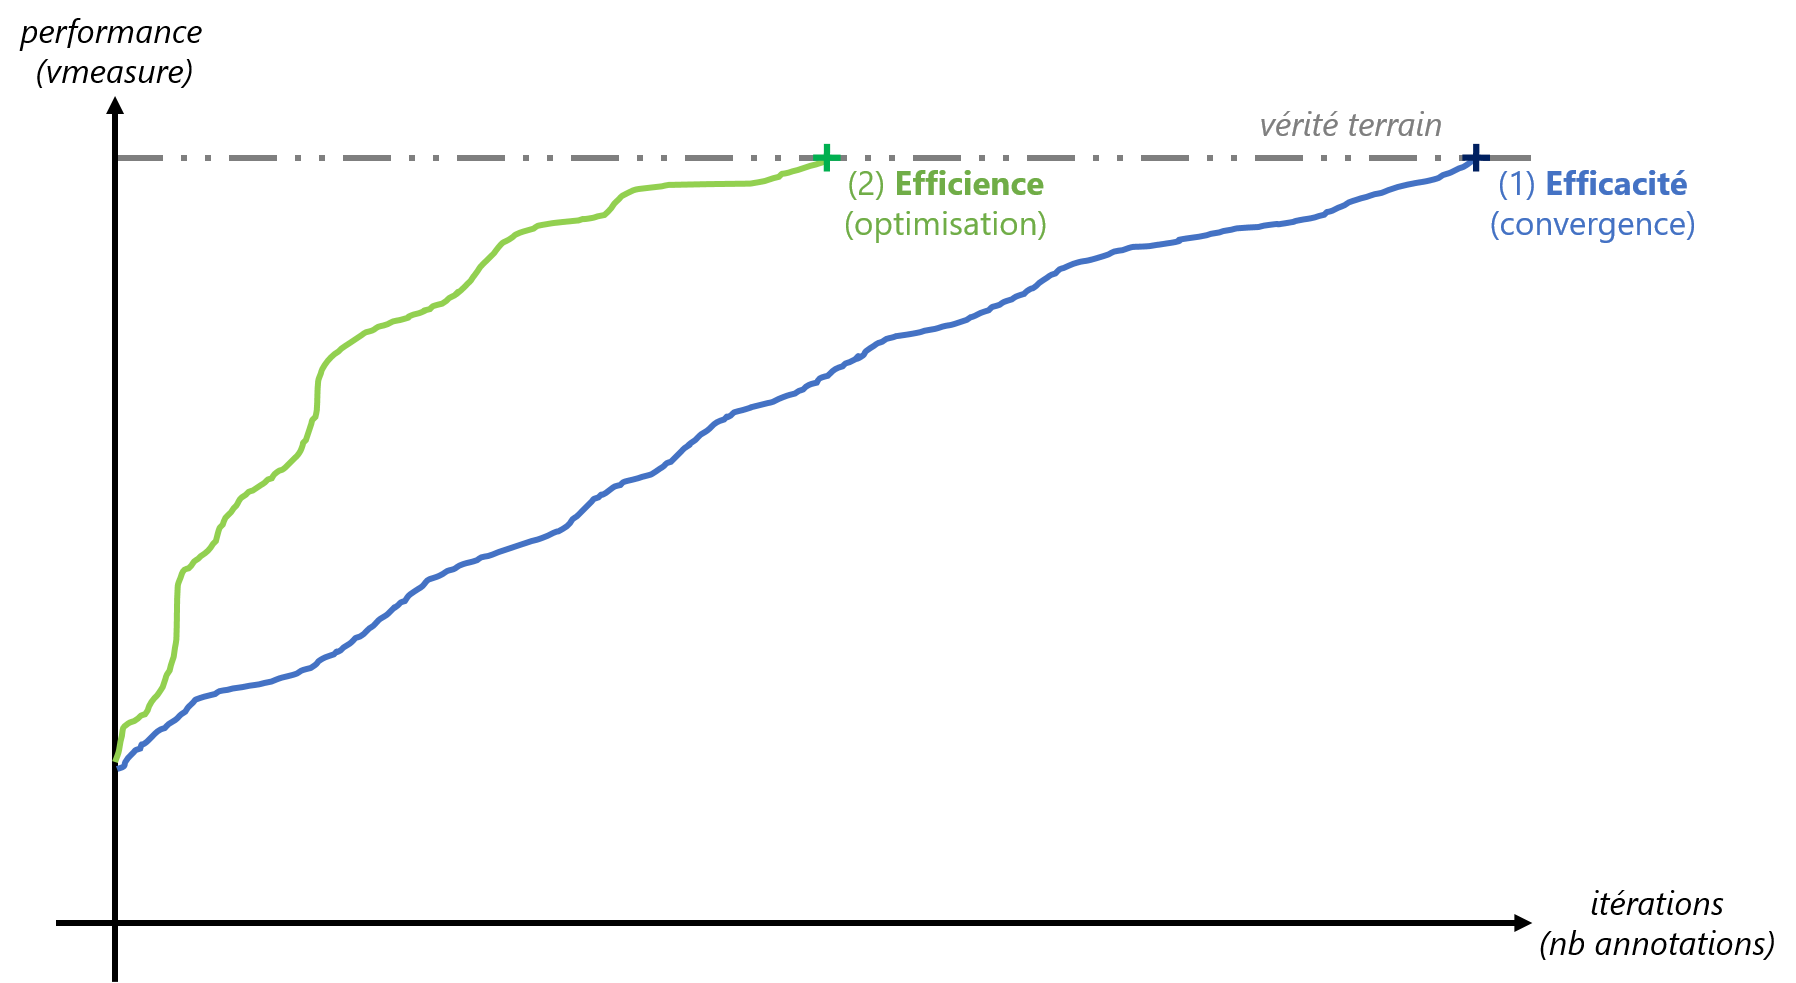
\includegraphics[width=0.95\textwidth]{figures/hypotheses-02-efficience}
			\caption{Illustration des études réalisées sur le \textit{clustering} interactif (\textit{étape 2/6}) en schématisant l'évolution de la performance (\textit{accord avec la vérité terrain calculé en v-measure}) d'une base d'apprentissage en cours de construction en fonction du nombre d'itérations de la méthode (\textit{nombre d'annotations par un expert métier}).}
			\label{figure:4.2-HYPOTHESE-EFFICIENCE}
		\end{figure}

	\end{tcolorbox}
	
	%%%
	%%% Subsection 4.2.1: Étude d'optimisation des paramètres d’implémentation en analysant leurs tailles d'effets sur la vitesse de création d'une base d'apprentissage.
	%%%
	\subsection{Étude d'optimisation des paramètres d’implémentation en analysant leurs tailles d'effets sur la vitesse de création d'une base d'apprentissage}
	\label{section:4.2.1-ETUDE-OPTIMISATION}
			
		% Référence articles.
		\begin{leftBarInformation}
			Cette étude a été l'objet d'une présentation à la conférence \texttt{EGC (Extraction et Gestion des Connaissances)}~\citep{schild:conception-interactive-clustering:2021}, et d'une extension dans le journal \texttt{IJDWM (International Journal of Data Warehousing and Mining)}~\citep{schild:extension-interactive-clustering:2022}.
			\footnote{Les résultats et la discussion de ces articles ont été mis à jour et réécrits pour mieux s'intégrer au discours ce manuscrit.}
		\end{leftBarInformation}

		%%% Protocole expérimental.
		\subsubsection{Protocole expérimental}

			% Objectif de l'expérience.
			Nous voulons étudier l'influence des paramètres de notre implémentation du \textit{clustering} interactif sur la vitesse de création d'une base d'apprentissage pour un assistant conversationnel.
			Nous allons donc compléter le protocole expérimental de l'étude de convergence en section~\ref{section:4.1.1-ETUDE-CONVERGENCE} visant à simuler la création d'une base d'apprentissage.
			
			% Axiome.
			\begin{leftBarWarning}
				Comme dans l'étude précédente, nous supposons que l'expert métier connaît parfaitement le domaine traité dans ce jeu de données, et qu'il est capable de caractériser sans ambiguïté la similitude entre deux données issues de cet ensemble.
				Cependant, cette hypothèse forte n'est pas toujours vérifiée en pratique, surtout lorsque l'on manipule des données non structurées.
				L'impact de ce point sur les résultats obtenus sera discuté en fin en fin de partie, et nous nous y intéresserons plus en détails dans la section~\ref{section:4.6-HYPOTHESE-ROBUSTESSE} (hypothèse de robustesse).
			\end{leftBarWarning}
			
			% Pseudo-code.
			Pour résumer le protocole expérimental adapté, vous pouvez vous référer au pseudo-code décrit dans Alg.~\ref{algorithm:4.2.1-ETUDE-OPTIMISATION-PROTOCOLE}.
			%
			\begin{algorithm}[!htb]
				\begin{algorithmic}[1]
					\Require jeu de données annoté (vérité terrain)
					\ForAll{arrangement d'algorithmes et de paramètres à tester}
						\State \textbf{initialisation (données)}: récupérer les données et la vérité terrain
						\State \textbf{initialisation (contraintes)}: créer une liste vide de contraintes
						\State \textbf{prétraitement}: supprimer le bruit dans les données
						\State \textbf{vectorisation}: transformer les données en vecteurs
						\State \textbf{clustering initial}: regrouper les données par similarité
						\State \textbf{évaluation}: estimer l'équivalence entre le \textit{clustering} obtenu et la vérité terrain
						\Repeat
							\State \textbf{échantillonnage}: sélectionner de nouvelles contraintes à annoter
							\State \textbf{simulation d'annotation}: ajouter des contraintes en utilisant la vérité terrain
							\State \textbf{clustering}: regrouper les données par similarité avec les contraintes
							\State \textbf{évaluation}: estimer l'équivalence entre le \textit{clustering} obtenu et la vérité terrain
						\Until{annotation de toutes les contraintes possibles}
					\EndFor
					\State \textbf{analyse}: déterminer les tailles d'effets des algorithmes et paramètres
					\Ensure meilleurs arrangements d'algorithmes et de paramètres
				\end{algorithmic}
				\caption{Description en pseudo-code du protocole expérimental de l'étude d'optimisation de la convergence du \textit{clustering} interactif vers une vérité terrain pré-établie.}
				\label{algorithm:4.2.1-ETUDE-OPTIMISATION-PROTOCOLE}
			\end{algorithm}
			
			% Détails de l'expérience.
			En s'appuyant sur les résultats précédemment obtenus,
			nous allons analyser l'influence des différentes tâches employées (\textbf{prétraitement}, \textbf{vectorisation}, \textbf{clustering sous contraintes}, \textbf{échantillonnage}) et de leurs paramètres sur la vitesse de convergence vers la vérité terrain.
			% Description implémentation de l'interactive clustering.
			Nous utilisons à nouveau le jeu de données \texttt{Bank Cards (v1.0.0)} (cf. annexe~\ref{annex:C.1-DATASET-BANK-CARDS}) comme vérité terrain, sur lequel nous testons $192$ combinaisons de paramétrage, et chaque tentative est répétée $5$ fois pour contrer les aléas statistiques de certains algorithmes.
			Pour plus de détails sur ces algorithmes, référez-vous à la section~\ref{section:3.3-DESCRIPTION-IMPLEMENTATION}.
			
			% Description de l'évaluation et Seuils d'évaluation.
			Comme lors de l'étude sur la convergence de la méthode, nous nous intéressons à l'évolution de la \texttt{v-measure} entre la vérité terrain et notre segmentation des données obtenue, et nous affinons notre évaluation en portant attention aux trois seuils d'annotations suivants :
			\begin{enumerate}
				\item le cas d'une \textbf{annotation partielle}, correspondant au nombre d'itérations nécessaires à la méthode pour avoir $90$\% de \texttt{v-measure}, c'est-à-dire un état de semi-parcours vers une convergence totale\footnote{Le seuil de $90$\% a été choisi au cours de l'étude de convergence (cf. hypothèse d'efficacité, section~\ref{section:4.1-HYPOTHESE-EFFICACITE}, coude de la figure~\ref{figure:4.1.1-ETUDE-CONVERGENCE-EVOLUTION}).} ;
				\item le cas d'une \textbf{annotation suffisante}, correspondant au nombre d'itérations nécessaires à la méthode pour avoir $100$\% de \texttt{v-measure}, c'est-à-dire avoir suffisamment de contraintes annotées par l'expert métier pour retrouver la vérité terrain ;
				\item le cas d'une \textbf{annotation exhaustive}, correspondant au nombre d'itérations nécessaires à la méthode pour parcourir toutes les contraintes possibles sur les données, et ainsi retranscrire exhaustivement la vision de l'expert métier\footnote{Une annotation est a priori inutilisable en pratique (demande trop de contraintes, cf. hypothèse d'efficacité, section~\ref{section:4.1-HYPOTHESE-EFFICACITE}), nous l'étudions toutefois pour avoir un point de comparaison.}.
			\end{enumerate}
			
			% Description de l'analyse ANOVA.
			Enfin, nous utilisons une \texttt{ANOVA} à mesures répétées afin de déterminer l’effet des paramètres de notre implémentation sur le nombre d’annotations requis pour converger vers la vérité terrain.
			
			% Référence scripts.
			\begin{leftBarInformation}
				Ces analyses sont réalisées à l'aide du logiciel R, et le test de \texttt{Tukey (HSD)} est utilisé pour les comparaisons post-hoc.
				Les scripts de l'expérience (\textit{notebooks} Python) sont disponibles dans un dossier dédié de~\cite{schild:cognitivefactory-interactive-clustering-comparative-study:2021}.
			\end{leftBarInformation}
			\todo{citation}

		%%% Résultats.
		\subsubsection{Résultats obtenus}
		
			%%% Analyse d'une annotation partielle.
			Pour obtenir une \textbf{annotation partielle} (\textit{atteindre une \texttt{v-measure} de $90$\%}), la moyenne des itérations est de $59.04$ (min: $11$, max: $315$, écart-type: $42.14$), soit une moyenne de $2~951.81$ annotations (min: $550$, max: $15~750$, écart-type: $2~106.72$).
			La figure~\ref{figure:4.2.1-ETUDE-OPTIMISATION-HISTOGRAMME-ANNOTATION-PARTIELLE} représente la répartition de ces itérations au cours des différentes tentatives.
			On peut noter les deux cas intéressants suivants :
			%
			\begin{itemize}
				\item[$\bullet$] Les tentatives les plus rapides furent celles avec un prétraitement des données \texttt{prep.no} ou \texttt{prep.simple} ou \texttt{prep.lemma}, une vectorisation des données \texttt{vect.tfidf}, un \textit{clustering} sous contraintes \texttt{clust.hier.sing}, et un échantillonnage de contraintes \texttt{samp.closest.diff}. Ces tentatives ont requis $11$ itérations, soit $550$ annotations, dont $299$ (respectivement $304$ et $281$) contraintes \texttt{MUST-LINK}.
				\item[$\bullet$] Les tentatives les plus lentes furent celles avec un prétraitement des données \texttt{prep.no}, une vectorisation des données \texttt{vect.tfidf}, un \textit{clustering} sous contraintes \texttt{clust.spec}, et un échantillonnage de contraintes \texttt{samp.farthest.same}. Ces tentatives ont requis $315$ itérations, soit $15~750$ annotations, dont $1~032$ contraintes \texttt{MUST-LINK}.
			\end{itemize}
			%
			\begin{figure}[!htb]
				\centering
				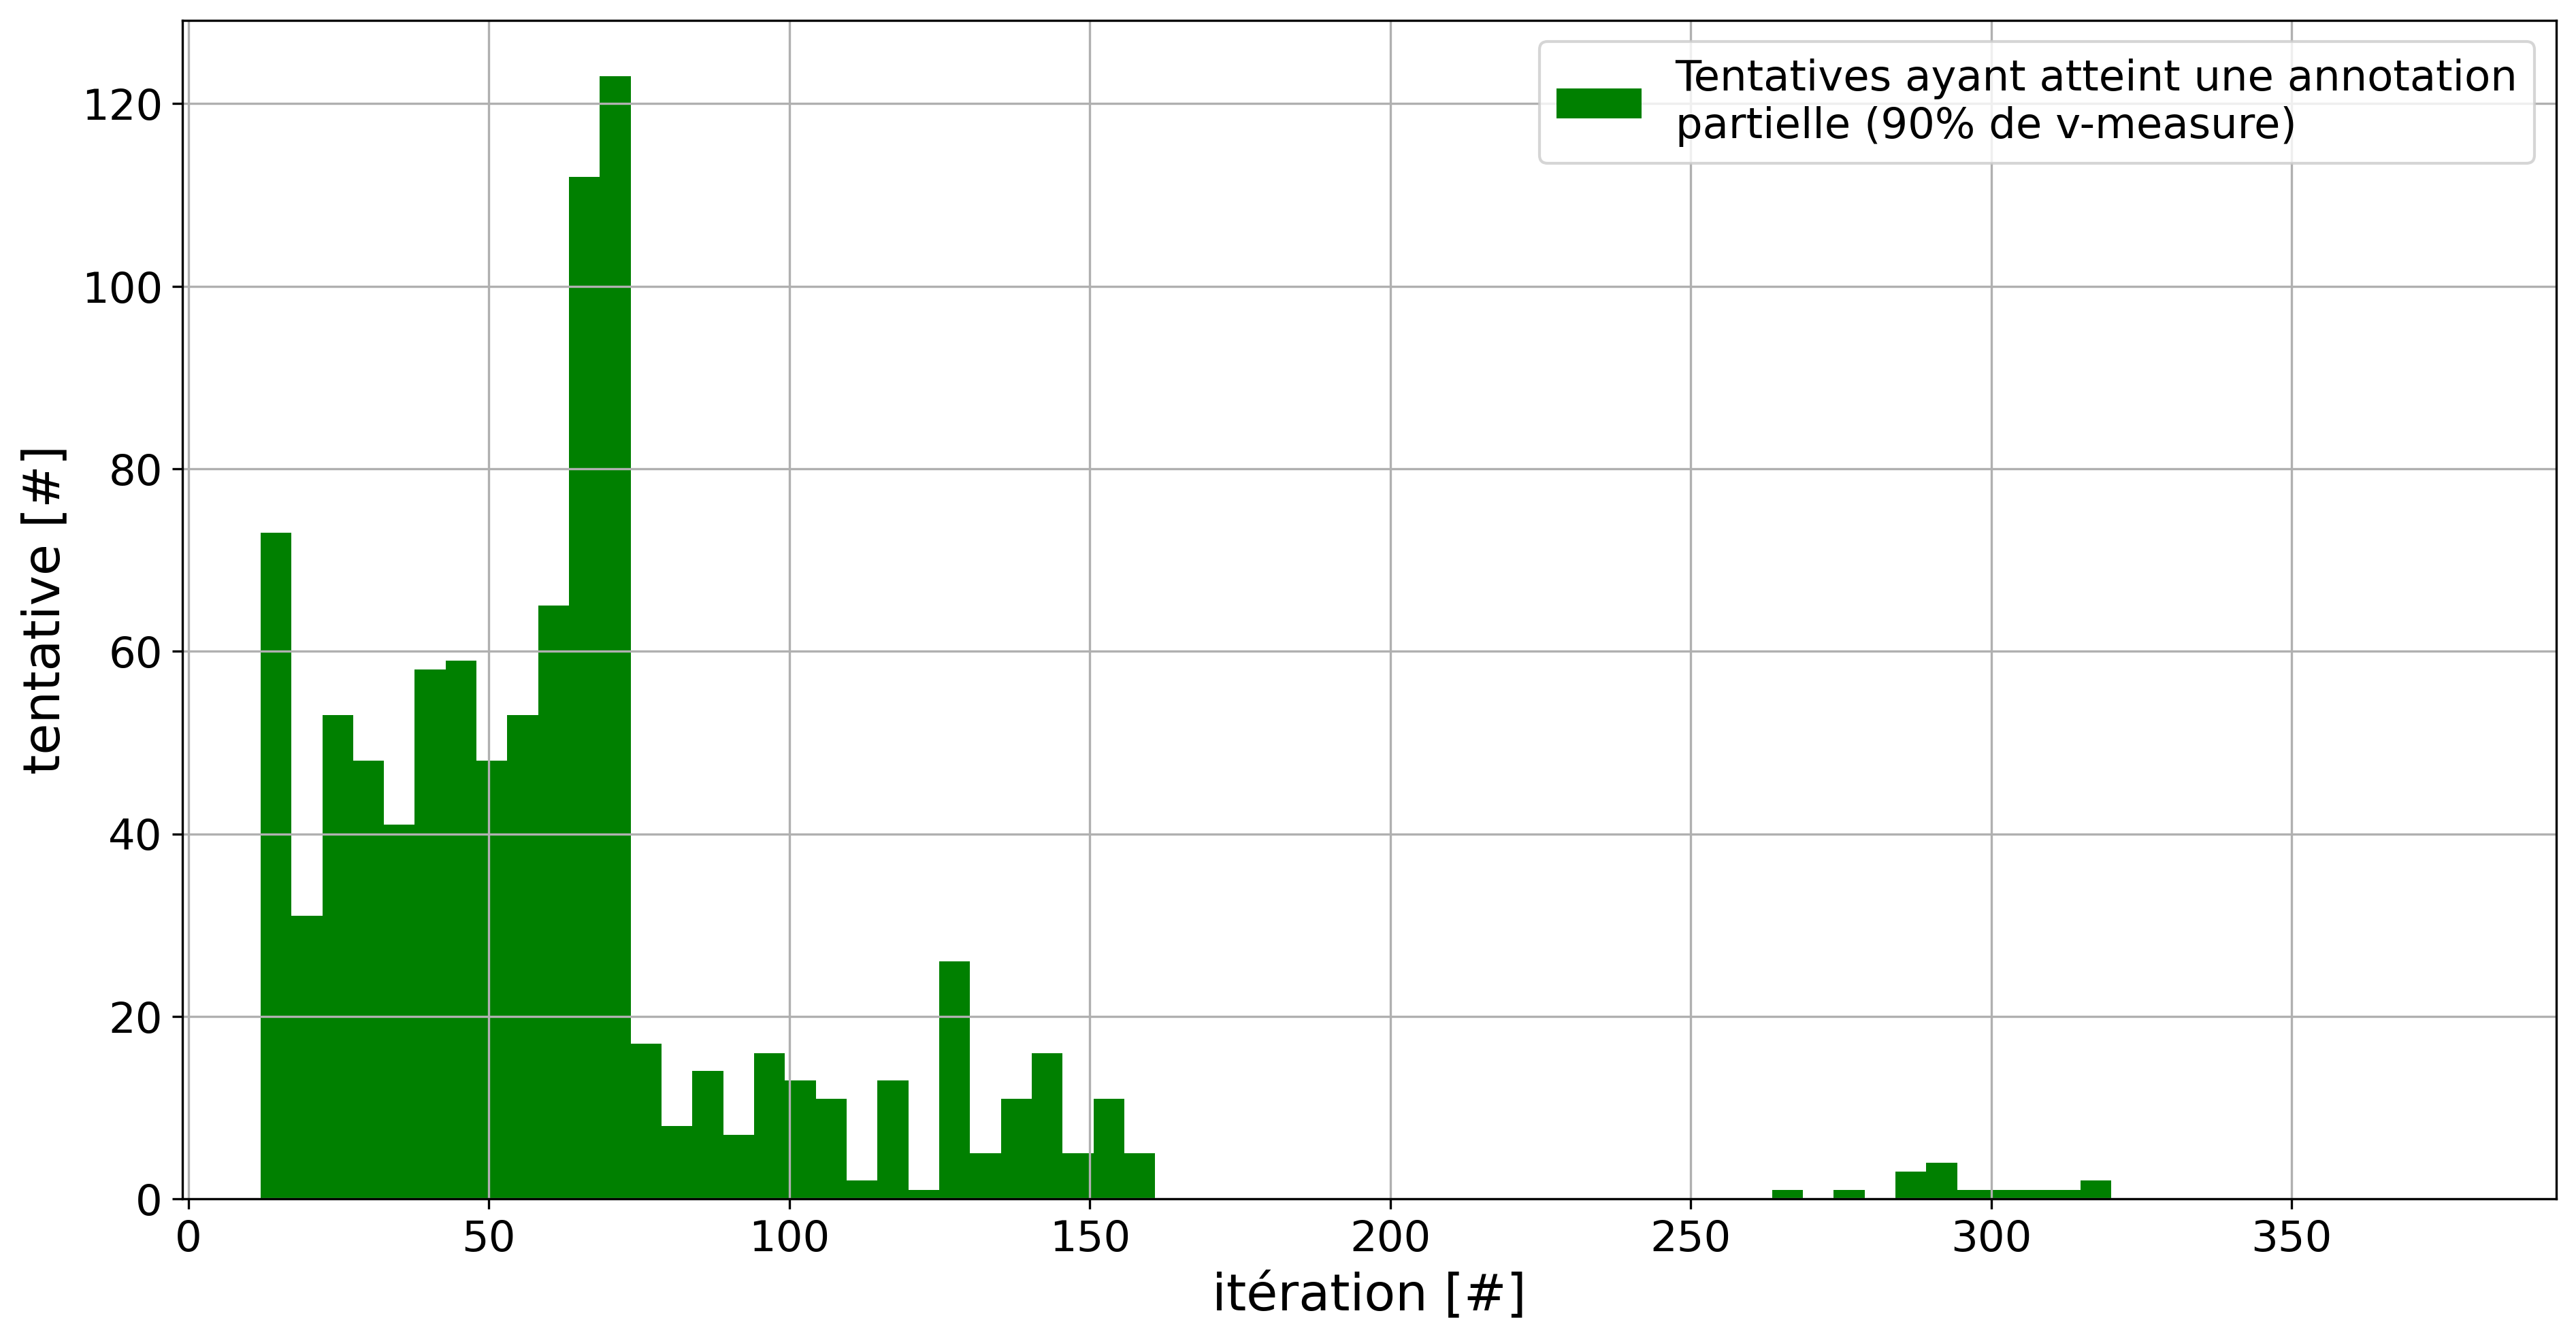
\includegraphics[width=0.95\textwidth]{figures/etude-efficience-histogramme-annotation-partielle}
				\caption{Répartition des tentatives en fonction de l'itération de la méthode à laquelle elles atteignent le seuil d'une annotation partielle, c'est-à-dire l'itération à laquelle elles parviennent à $90$\% de \texttt{v-measure} entre un résultat obtenu et la vérité terrain. L'histogramme est réduit à $60$ pics pour simplifier l'affichage.}
				\label{figure:4.2.1-ETUDE-OPTIMISATION-HISTOGRAMME-ANNOTATION-PARTIELLE}
			\end{figure}
			%
			Le tableau~\ref{table:4.2.1-ETUDE-OPTIMISATION-ANOVA-ANNOTATION-PARTIELLE} retranscrit l'influence de chacun des paramètres sur le nombre d'itérations nécessaires pour atteindre une \textbf{annotation partielle} (\textit{atteindre une \texttt{v-measure} de $90$\%}).
			Les analyses de variance mettent en relief l'effet significatif sur cette convergence du prétraitement (\texttt{eta-carré}: $0.320$, \texttt{p-valeur}: $< 10^{-3}$), de la vectorisation (\texttt{eta-carré}: $0.388$, \texttt{p-valeur}: $< 10^{-3}$), du \textit{clustering} (\texttt{eta-carré}: $0.866$, \texttt{p-valeur}: $< 10^{-3}$) et de l'échantillonnage (\texttt{eta-carré}: $0.968$, \texttt{p-valeur}: $< 10^{-3}$).
			L'analyse post-hoc de ces effets indique que le meilleur paramétrage moyen pour atteindre une \textbf{annotation partielle} repose sur la prétraitement \texttt{prep.simple}, le vectorisation \texttt{vect.tfidf}, le \textit{clustering} \texttt{clust.hier.avg}, et l'échantillonnage \texttt{samp.closest.diff}. La moyenne du nombre d'itération requis pour ce paramétrage est de $19.00$ (écart-type: $0.79$), soit $950$ annotations (écart-type: $39.34$).
			%
			\begin{table}[!htb]
				\begin{center}
				\begin{tabular}{|c|c|c|c|c|c|c|}
					\hline
					% ENTETE DU TABLEAU
					\multicolumn{2}{|c|}{ \shortstack{Description des \\ facteurs analysés } }
						& \multicolumn{3}{c|}{ \shortstack{ Description statistique \\ des itérations } }
						& \multicolumn{2}{c|}{ \shortstack{ Description des \\ tailles d'effets } }
						\tabularnewline
						\hline

					Facteur
						& Niveau 
						& Moyenne
						& Rang
						& SE
						& \texttt{ $ \eta^{2} $ }
						& \texttt{p-valeur}
						\tabularnewline
						\hline
					
					% PRETRAITEMENT
					\multirow{4}{*}{prétraitement}
						& \texttt{prep.simple}
						& $61.90$
						& (1)
						& \multirow{4}{*}{ $0.32$ }
						& \multirow{4}{*}{ $0.320$ }
						& \multirow{4}{*}{ \shortstack{ $< 10^{-3}$ \\ ($***$) } }
						\tabularnewline
						\cline{2-4}
						
						& \texttt{prep.lemma}
						& $63.08$
						& (2)
						&
						&
						&
						\tabularnewline
						\cline{2-4}
						
						& \texttt{prep.no}
						& $63.70$
						& (2)
						&
						& 
						&
						\tabularnewline
						\cline{2-4}
						
						& \texttt{prep.filter}
						& $71.90$
						& (4)
						&
						&
						&
						\tabularnewline
						\hline
					
					% VECTORISATION
					\multirow{2}{*}{vectorisation}
						& \texttt{vect.tfidf}
						& $60.61$
						& (1)
						& \multirow{2}{*}{ $0.29$ }
						& \multirow{2}{*}{ $0.388$ }
						& \multirow{2}{*}{ \shortstack{$< 10^{-3}$ \\ ($***$) } }
						\tabularnewline
						\cline{2-4}
						
						& \texttt{vect.frcorenewsmd}
						& $63.08$
						& (2)
						&
						&
						&
						\tabularnewline
						\hline
					
					% CLUSTERING
					\multirow{6}{*}{clustering}
						& \texttt{clust.hier.avg}
						& $50.64$
						& (1)
						& \multirow{6}{*}{ $0.35$ }
						& \multirow{6}{*}{ $0.866$ }
						& \multirow{6}{*}{ \shortstack{ $< 10^{-3}$ \\ ($***$) } }
						\tabularnewline
						\cline{2-4}
						
						& \texttt{clust.kmeans.cop}
						& $52.43$
						& (2)
						&
						&
						&
						\tabularnewline
						\cline{2-4}
						
						& \texttt{clust.hier.sing}
						& $54.08$
						& (3)
						&
						& 
						&
						\tabularnewline
						\cline{2-4}
						
						& \texttt{clust.hier.ward}
						& $72.41$
						& (4)
						&
						& 
						&
						\tabularnewline
						\cline{2-4}
						
						& \texttt{clust.hier.comp}
						& $73.48$
						& (5)
						&
						&
						&
						\tabularnewline
						\cline{2-4}
						
						& \texttt{clust.spec}
						& $87.84$
						& (6)
						&
						& 
						&
						\tabularnewline
						\hline
					
					% ECHANTILLONNAGE
					\multirow{4}{*}{échantillonnage}
						& \texttt{samp.closest.diff}
						& $33.66$
						& (1)
						& \multirow{4}{*}{ $0.32$ }
						& \multirow{4}{*}{ $0.968$ }
						& \multirow{4}{*}{ \shortstack{ $< 10^{-3}$ \\ ($***$) } }
						\tabularnewline
						\cline{2-4}
						
						& \texttt{samp.random.same}
						& $48.24$
						& (2)
						&
						&
						&
						\tabularnewline
						\cline{2-4}
						
						& \texttt{samp.random.full}
						& $65.83$
						& (3)
						&
						& 
						&
						\tabularnewline
						\cline{2-4}
						
						& \texttt{samp.farhtest.same}
						& $112.86$
						& (4)
						&
						&
						&
						\tabularnewline
						\hline
				\end{tabular}
				\end{center}
				\caption{ANOVA du nombre d'itérations nécessaires pour l'obtention de $90$\% de v-mesure. Les (\textit{$*$}) dénotent le niveau de significativité ($\alpha=0.05$). Pour les effets significatifs, les chiffres précisés entre parenthèses dans la colonne \texttt{Moyenne} indiquent le classement des niveaux selon les analyses post-hoc.}
				\label{table:4.2.1-ETUDE-OPTIMISATION-ANOVA-ANNOTATION-PARTIELLE}
			\end{table}
			

			%%% Analyse d'une annotation suffisante.
			Pour obtenir une \textbf{annotation suffisante} (\textit{atteindre une \texttt{v-measure} de $100$\%}), la moyenne des itérations est de $76.29$ (min: $19$, max: $328$, écart-type: $46.44$), soit une moyenne de $3~801.19$ annotations (min: $950$, max: $16~400$, écart-type: $2~314.91$).
			La figure~\ref{figure:4.2.1-ETUDE-OPTIMISATION-HISTOGRAMME-ANNOTATION-SUFFISANTE} représente la répartition de ces itérations au cours des différentes tentatives.
			On peut noter les deux cas intéressants suivants :
			%
			\begin{itemize}
				\item[$\bullet$] Les tentatives les plus rapides furent celles avec un prétraitement des données \texttt{prep.simple}, une vectorisation des données \texttt{vect.tfidf}, un \textit{clustering} sous contraintes \texttt{clust.hier.comp} ou \texttt{clust.hier.ward}, et un échantillonnage de contraintes \texttt{samp.closest.diff}. Ces tentatives ont requis $19$ itérations, soit $950$ annotations, dont $638$ (respectivement $641$) contraintes \texttt{MUST-LINK}.
				\item[$\bullet$] Les tentatives les plus lentes furent celles avec un prétraitement des données \texttt{prep.no}, une vectorisation des données \texttt{vect.tfidf}, un \textit{clustering} sous contraintes \texttt{clust.spec}, et un échantillonnage de contraintes \texttt{samp.farthest.same}. Ces tentatives ont requis $394$ itérations, soit $16~400$ annotations, dont $1~309$ contraintes \texttt{MUST-LINK}.
			\end{itemize}
			%
			\begin{figure}[!htb]
				\centering
				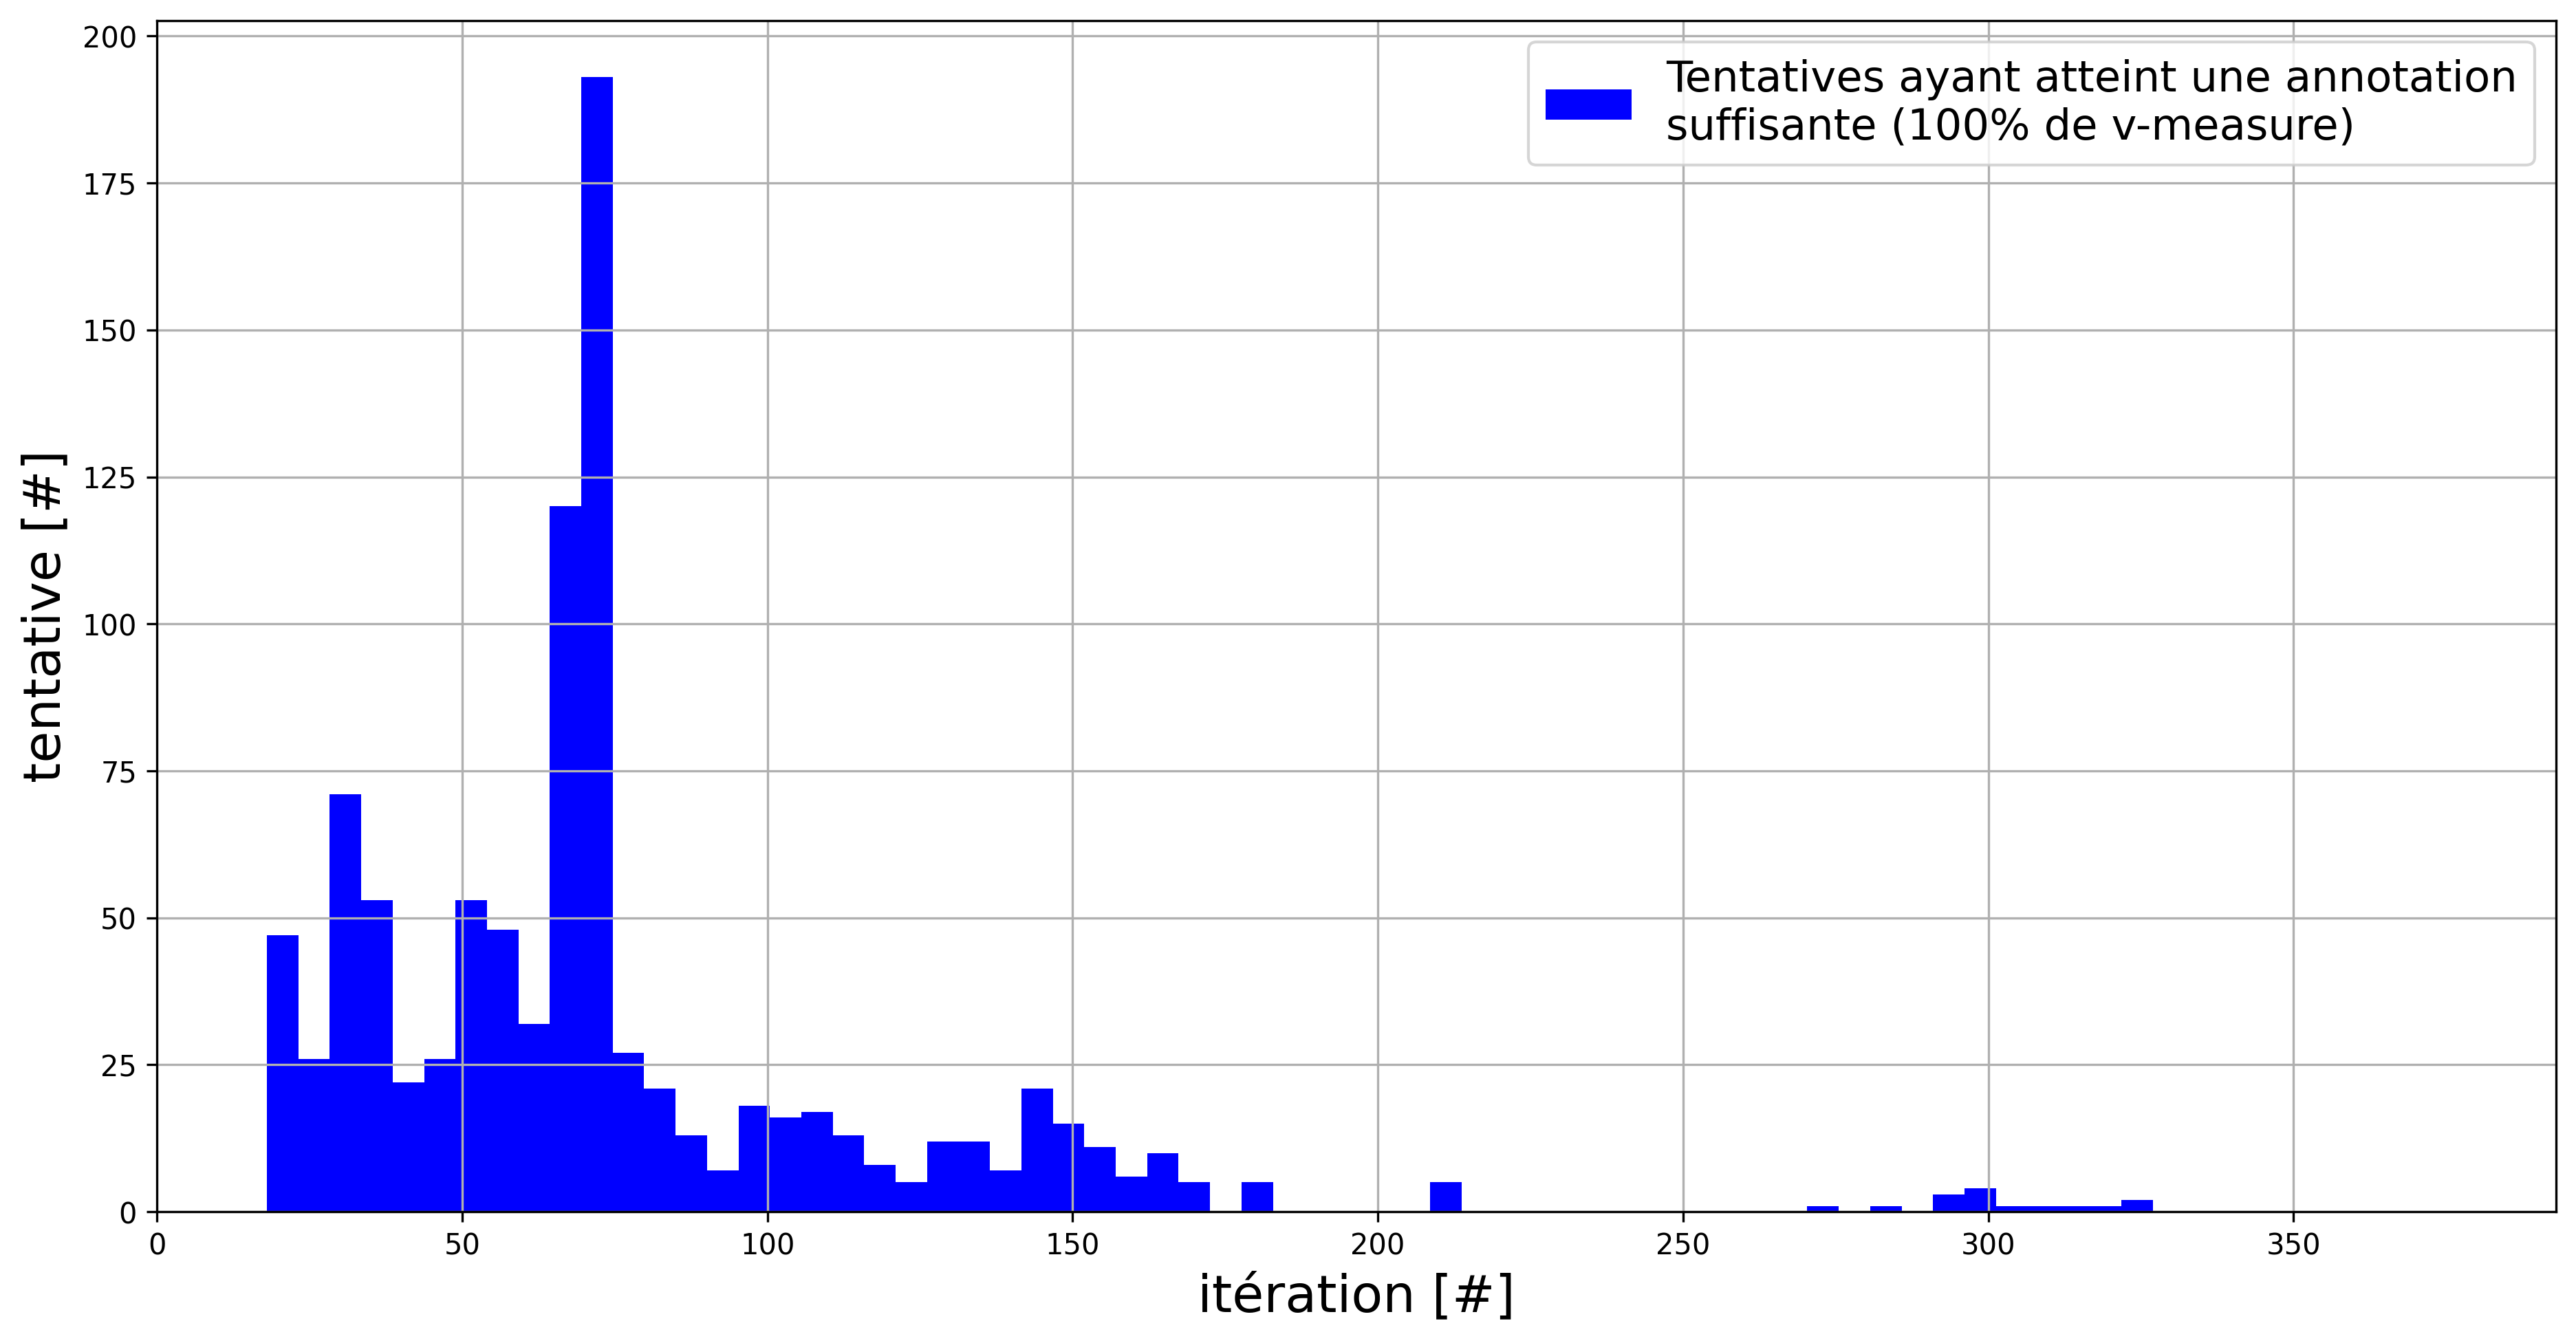
\includegraphics[width=0.95\textwidth]{figures/etude-efficience-histogramme-annotation-suffisante}
				\caption{Répartition des tentatives en fonction de l'itération de la méthode à laquelle elles atteignent le seuil d'une annotation suffisante, c'est-à-dire l'itération à laquelle elles parviennent à $100$\% de \texttt{v-measure} entre un résultat obtenu et la vérité terrain. L'histogramme est réduit à $60$ pics pour simplifier l'affichage.}
				\label{figure:4.2.1-ETUDE-OPTIMISATION-HISTOGRAMME-ANNOTATION-SUFFISANTE}
			\end{figure}
			%
			Le tableau~\ref{table:4.2.1-ETUDE-OPTIMISATION-ANOVA-ANNOTATION-SUFFISANTE} retranscrit l'influence de chacun des paramètres sur le nombre d'itérations nécessaires pour atteindre une \textbf{annotation suffisante}.
			Les analyses de variance mettent en relief l'effet significatif sur cette convergence du prétraitement (\texttt{eta-carré}: $0.987$, \texttt{p-valeur}: $< 10^{-3}$), de la vectorisation (\texttt{eta-carré}: $0.991$, \texttt{p-valeur}: $< 10^{-3}$), du \textit{clustering} (\texttt{eta-carré}: $0.997$, \texttt{p-valeur}: $< 10^{-3}$) et de l'échantillonnage (\texttt{eta-carré}: $0.998$, \texttt{p-valeur}: $< 10^{-3}$).
			L'analyse post-hoc de ces effets indique que le meilleur paramétrage moyen pour atteindre une \textbf{annotation suffisante} repose sur la prétraitement \texttt{prep.lemma}, le vectorisation \texttt{vect.tfidf}, le \textit{clustering} \texttt{clust.kmeans.cop}, et l'échantillonnage \texttt{samp.closest.diff}. La moyenne du nombre d'itération requis pour ce paramétrage est de $34.60$ (écart-type: $7.44$), soit $1~730$ annotations (écart-type: $372.00$).
			%
			\begin{table}[!htb]
				\begin{center}
				\begin{tabular}{|c|c|c|c|c|c|c|}
					\hline
					% ENTETE DU TABLEAU
					\multicolumn{2}{|c|}{ \shortstack{Description des \\ facteurs analysés } }
						& \multicolumn{3}{c|}{ \shortstack{ Description statistique \\ des itérations } }
						& \multicolumn{2}{c|}{ \shortstack{ Description des \\ tailles d'effets } }
						\tabularnewline
						\hline

					Facteur
						& Niveau 
						& Moyenne
						& Rang
						& SE
						& \texttt{ $\eta^{2}$ }
						& \texttt{p-valeur}
						\tabularnewline
						\hline
					
					% PRETRAITEMENT
					\multirow{4}{*}{prétraitement}
						& \texttt{prep.lemma}
						& $72.86$
						& (1)
						& \multirow{4}{*}{ $0.32$ }
						& \multirow{4}{*}{ $0.276$ }
						& \multirow{4}{*}{ \shortstack{ $< 10^{-3}$ \\ ($***$) } }
						\tabularnewline
						\cline{2-4}
						
						& \texttt{prep.simple}
						& $73.30$
						& (2)
						&
						&
						&
						\tabularnewline
						\cline{2-4}
						
						& \texttt{prep.no}
						& $75.24$
						& (2)
						&
						& 
						&
						\tabularnewline
						\cline{2-4}
						
						& \texttt{prep.filter}
						& $83.77$
						& (4)
						&
						&
						&
						\tabularnewline
						\hline
					
					% VECTORISATION
					\multirow{2}{*}{vectorisation}
						& \texttt{vect.tfidf}
						& $71.16$
						& (1)
						& \multirow{2}{*}{ $0.36$ }
						& \multirow{2}{*}{ $0.366$ }
						& \multirow{2}{*}{ \shortstack{$< 10^{-3}$ \\ ($***$)} }
						\tabularnewline
						\cline{2-4}
						
						& \texttt{vect.frcorenewsmd}
						& $81.43$
						& (2)
						&
						&
						&
						\tabularnewline
						\hline
					
					% CLUSTERING
					\multirow{6}{*}{clustering}
						& \texttt{clust.kmeans.cop}
						& $62.23$
						& (1)
						& \multirow{6}{*}{ $0.42$ }
						& \multirow{6}{*}{ $0.700$ }
						& \multirow{6}{*}{ \shortstack{$< 10^{-3}$ \\ ($***$)} }
						\tabularnewline
						\cline{2-4}
						
						& \texttt{clust.hier.avg}
						& $65.13$
						& (2)
						&
						&
						&
						\tabularnewline
						\cline{2-4}
						
						& \texttt{clust.hier.sing}
						& $75.44$
						& (3)
						&
						& 
						&
						\tabularnewline
						\cline{2-4}
						
						& \texttt{clust.hier.ward}
						& $80.44$
						& (4)
						&
						& 
						&
						\tabularnewline
						\cline{2-4}
						
						& \texttt{clust.hier.comp}
						& $81.46$
						& (5)
						&
						&
						&
						\tabularnewline
						\cline{2-4}
						
						& \texttt{clust.spec}
						& $93.06$
						& (6)
						&
						& 
						&
						\tabularnewline
						\hline
					
					% ECHANTILLONNAGE
					\multirow{4}{*}{échantillonnage}
						& \texttt{samp.closest.diff}
						& $50.29$
						& (1)
						& \multirow{4}{*}{ $0.39$ }
						& \multirow{4}{*}{ $0.950$ }
						& \multirow{4}{*}{ \shortstack{$< 10^{-3}$ \\ ($***$)} }
						\tabularnewline
						\cline{2-4}
						
						& \texttt{samp.random.same}
						& $56.38$
						& (2)
						&
						&
						&
						\tabularnewline
						\cline{2-4}
						
						& \texttt{samp.random.full}
						& $71.95$
						& (3)
						&
						& 
						&
						\tabularnewline
						\cline{2-4}
						
						& \texttt{samp.farhtest.same}
						& $126.55$
						& (4)
						&
						&
						&
						\tabularnewline
						\hline
				\end{tabular}
				\end{center}
				\caption{ANOVA du nombre d'itérations nécessaires pour l'obtention de $100$\% de v-mesure. Les (\textit{$*$}) dénotent le niveau de significativité ($\alpha=0.05$). Pour les effets significatifs, les chiffres précisés entre parenthèses dans la colonne \texttt{Moyenne} indiquent le classement des niveaux selon les analyses post-hoc.}
				\label{table:4.2.1-ETUDE-OPTIMISATION-ANOVA-ANNOTATION-SUFFISANTE}
			\end{table}
			
			%%% Analyse d'une annotation exhaustive.
			Enfin, pour avoir une \textbf{annotation exhaustive} (\textit{annoter toutes les contraintes possibles}), la moyenne des itérations est de $88.98$ (min: $20$, max: $394$, écart-type: $68.21$), soit une moyenne de $4~431.34$ annotations (min: $1~000$, max: $19~656$, écart-type: $3~405.16$).
			La figure~\ref{figure:4.2.1-ETUDE-OPTIMISATION-HISTOGRAMME-ANNOTATION-EXHAUSTIVE} représente la répartition de ces itérations au cours des différentes tentatives.
			On peut noter les deux cas intéressants suivant :
			%
			\begin{itemize}
				\item[$\bullet$] Les tentatives les plus rapides furent celles avec un prétraitement des données \texttt{prep.no} ou \texttt{prep.lemma}, une vectorisation des données \texttt{vect.tfidf}, un algorithme de \textit{clustering} sous contraintes \texttt{clust.hier.comp} ou \texttt{clust.hier.ward}, et un échantillonnage de contraintes \texttt{samp.closest.diff}. Ces tentatives ont requis $20$ itérations, soit $1~000$ annotations, dont $653$ (respectivement $668$) contraintes \texttt{MUST-LINK}.
				\item[$\bullet$] Les tentatives les plus lentes furent celles avec un prétraitement des données \texttt{prep.simple}, une vectorisation des données \texttt{vect.frcorenewsmd}, un \textit{clustering} \texttt{clust.hier.sing}, et un échantillonnage de contraintes \texttt{samp.closest.diff}. Ces tentatives ont requis $394$ itérations, soit $19~656$ annotations, dont $682$ contraintes \texttt{MUST-LINK}.
			\end{itemize}
			%
			\begin{figure}[!htb]
				\centering
				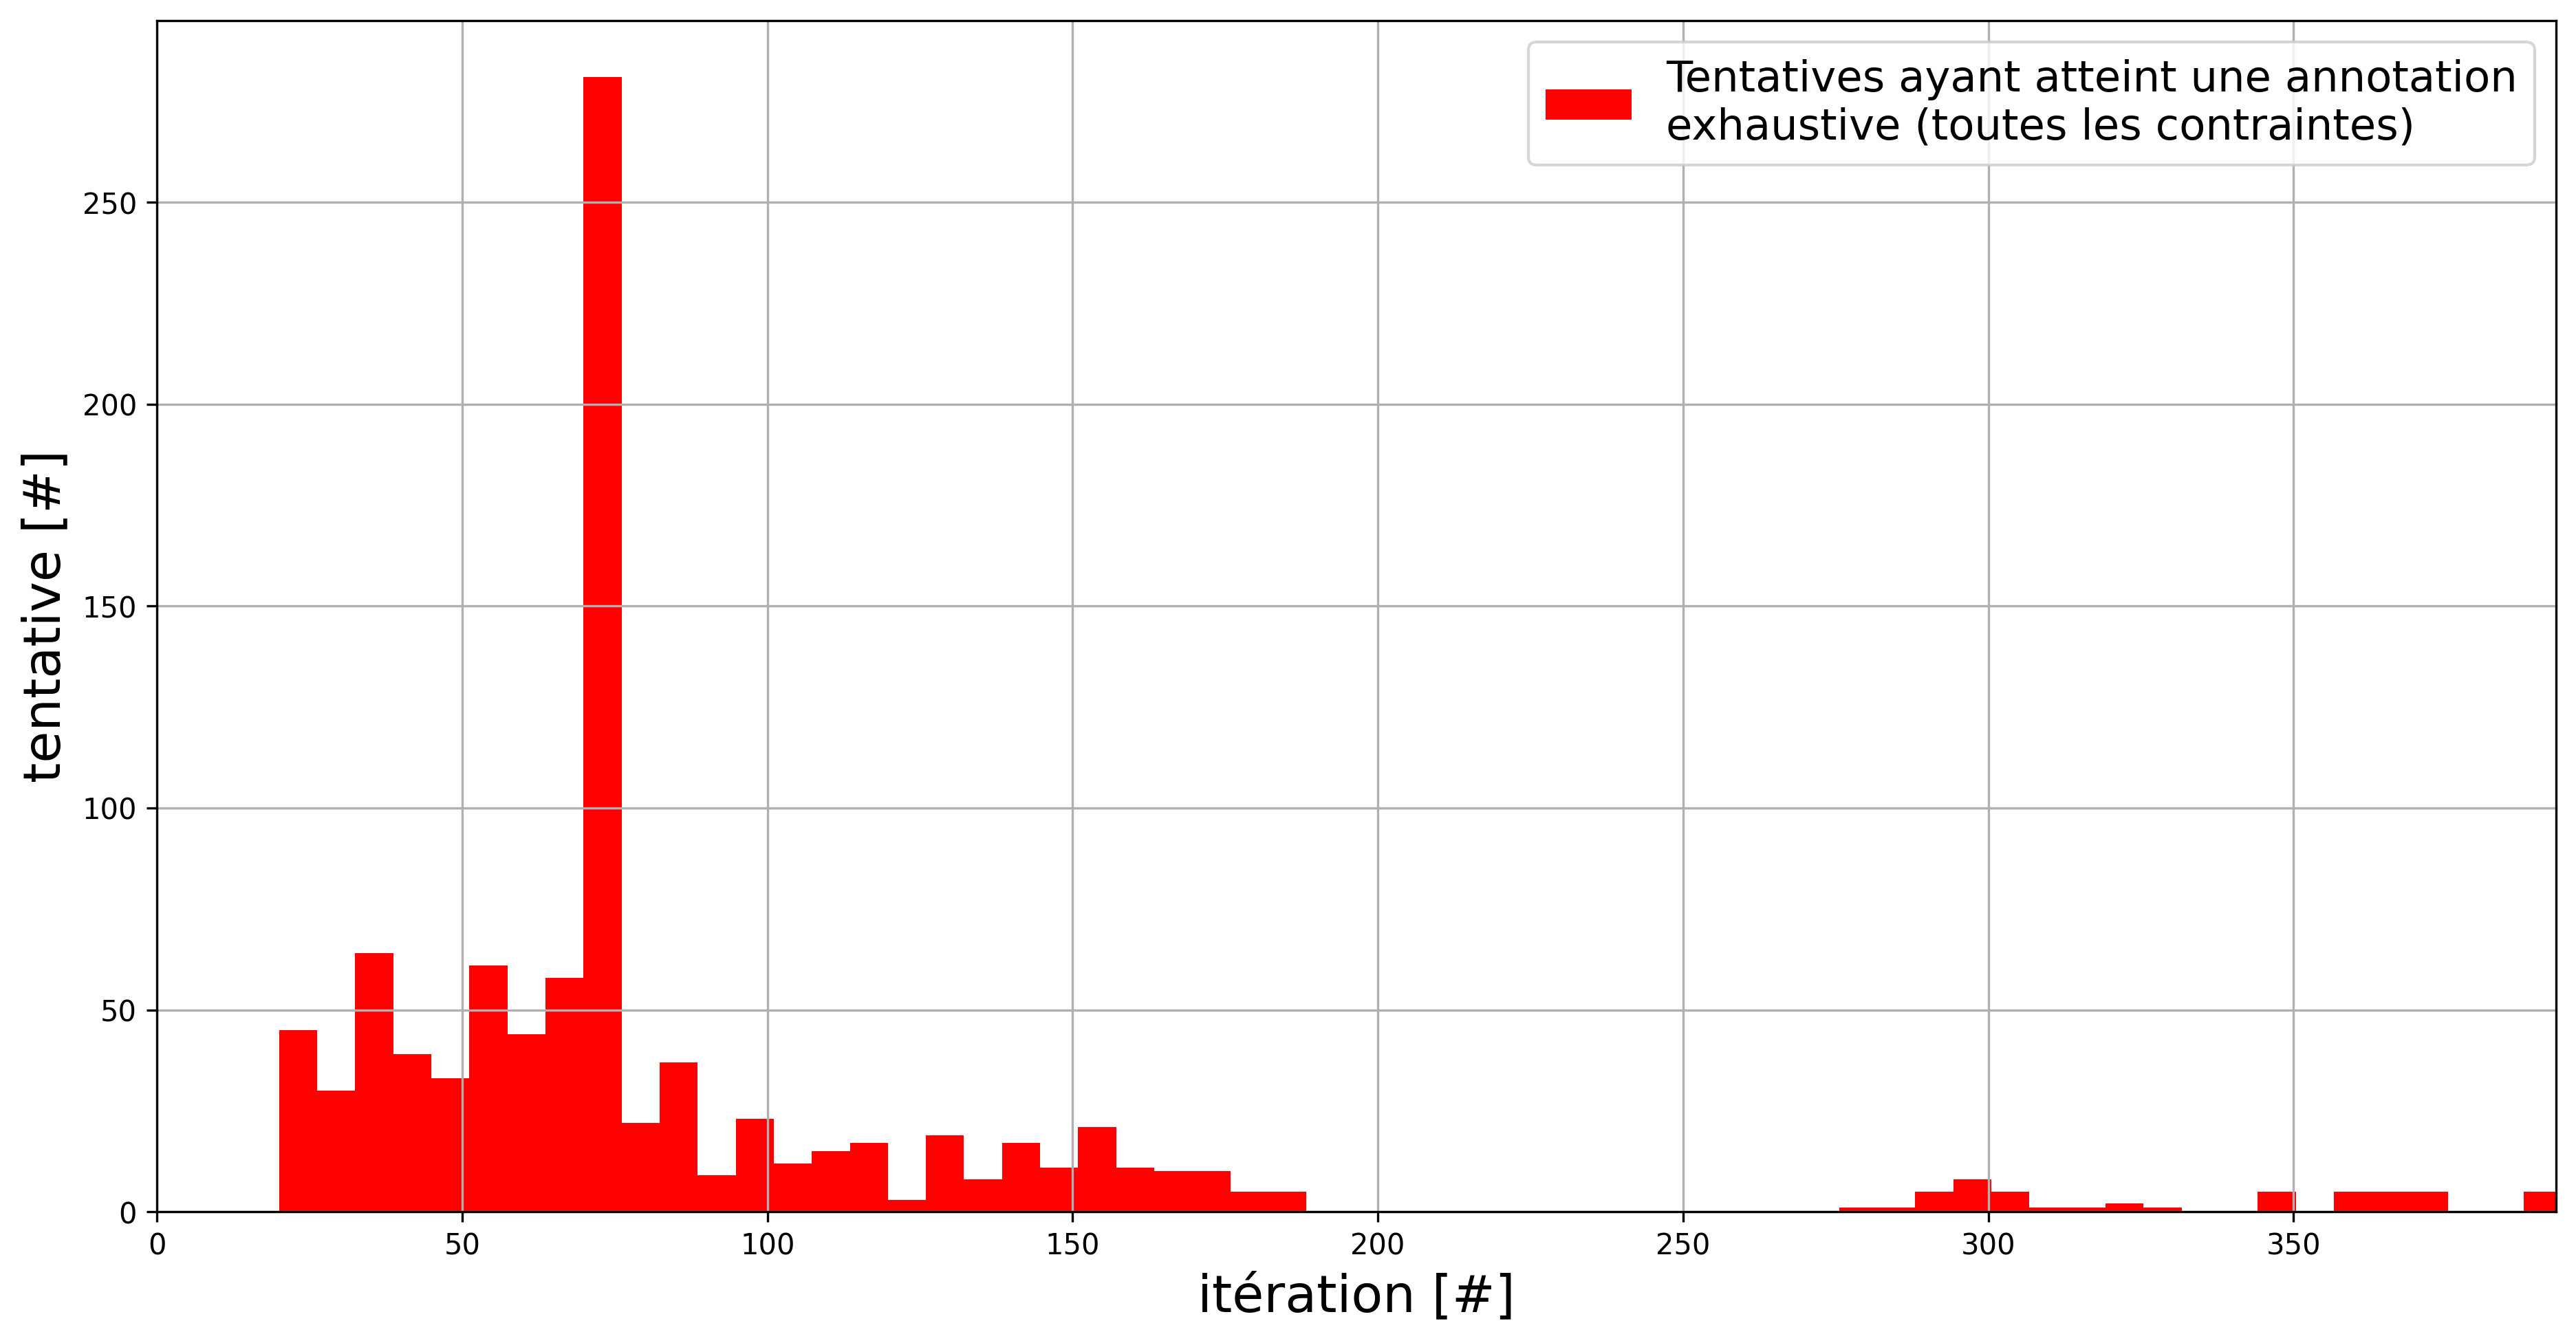
\includegraphics[width=0.95\textwidth]{figures/etude-efficience-histogramme-annotation-exhaustive}
				\caption{Répartition des tentatives en fonction de l'itération de la méthode à laquelle elles atteignent le seuil d'une annotation exhaustive, c'est-à-dire l'itération à laquelle toutes les contraintes possibles entre les données ont été annotées. L'histogramme est réduit à $60$ pics pour simplifier l'affichage.}
				\label{figure:4.2.1-ETUDE-OPTIMISATION-HISTOGRAMME-ANNOTATION-EXHAUSTIVE}
			\end{figure}
			%
			Le tableau~\ref{table:4.2.1-ETUDE-OPTIMISATION-ANOVA-ANNOTATION-EXHAUSTIVE} retranscrit l'influence de chacun des paramètres sur le nombre d'itérations nécessaires pour atteindre une \textbf{annotation exhaustive}.
			Les analyses de variance mettent en relief l'effet significatif sur cette convergence du prétraitement (\texttt{eta-carré}: $0.909$, \texttt{p-valeur}: $< 10^{-3}$), de la vectorisation (\texttt{eta-carré}: $0.985$, \texttt{p-valeur}: $< 10^{-3}$), du \textit{clustering} (\texttt{eta-carré}: $0.999$, \texttt{p-valeur}: $< 10^{-3}$) et de l'échantillonnage (\texttt{eta-carré}: $0.997$, \texttt{p-valeur}: $< 10^{-3}$).
			L'analyse post-hoc de ces effets indique que le meilleur paramétrage moyen pour atteindre une \textbf{annotation exhaustive} repose sur la prétraitement \texttt{prep.lemma}, le vectorisation \texttt{vect.tfidf}, le \textit{clustering} \texttt{clust.kmeans.cop}, et l'échantillonnage \texttt{samp.random.same}. La moyenne du nombre d'itération requis pour ce paramétrage est de $32.60$ (écart-type: $1.14$), soit $1~630$ annotations (écart-type: $57.00$).
			%
			\begin{table}[!htb]
				\begin{center}
				\begin{tabular}{|c|c|c|c|c|c|c|}
					\hline
					% ENTETE DU TABLEAU
					\multicolumn{2}{|c|}{ \shortstack{Description des \\ facteurs analysés } }
						& \multicolumn{3}{c|}{ \shortstack{ Description statistique \\ des itérations } }
						& \multicolumn{2}{c|}{ \shortstack{ Description des \\ tailles d'effets } }
						\tabularnewline
						\hline

					Facteur
						& Niveau 
						& Moyenne
						& Rang
						& SE
						& \texttt{ $\eta^{2}$ }
						& \texttt{p-valeur}
						\tabularnewline
						\hline
					
					% PRETRAITEMENT
					\multirow{4}{*}{prétraitement}
						& \texttt{prep.lemma}
						& $85.89$
						& (1)
						& \multirow{4}{*}{ $0.42$ }
						& \multirow{4}{*}{ $0.052$ }
						& \multirow{4}{*}{ \shortstack{$< 10^{-3}$ \\ ($***$)} }
						\tabularnewline
						\cline{2-4}
						
						& \texttt{prep.filter}
						& $89.55$
						& (2)
						&
						&
						&
						\tabularnewline
						\cline{2-4}
						
						& \texttt{prep.simple}
						& $89.64$
						& (2)
						&
						& 
						&
						\tabularnewline
						\cline{2-4}
						
						& \texttt{prep.no}
						& $90.81$
						& (4)
						&
						&
						&
						\tabularnewline
						\hline
					
					% VECTORISATION
					\multirow{2}{*}{vectorisation}
						& \texttt{vect.tfidf}
						& $85.50$
						& (1)
						& \multirow{2}{*}{ $0.39$ }
						& \multirow{2}{*}{ $0.165$ }
						& \multirow{2}{*}{ \shortstack{$< 10^{-3}$ \\ ($***$)} }
						\tabularnewline
						\cline{2-4}
						
						& \texttt{vect.frcorenewsmd}
						& $92.46$
						& (2)
						&
						&
						&
						\tabularnewline
						\hline
					
					% CLUSTERING
					\multirow{6}{*}{clustering}
						& \texttt{clust.kmeans.cop}
						& $64.99$
						& (1)
						& \multirow{6}{*}{ $0.39$ }
						& \multirow{6}{*}{ $0.894$ }
						& \multirow{6}{*}{ \shortstack{$< 10^{-3}$ \\ ($***$)} }
						\tabularnewline
						\cline{2-4}
						
						& \texttt{clust.hier.avg}
						& $78.54$
						& (2)
						&
						&
						&
						\tabularnewline
						\cline{2-4}
						
						& \texttt{clust.hier.ward}
						& $81.31$
						& (3)
						&
						& 
						&
						\tabularnewline
						\cline{2-4}
						
						& \texttt{clust.hier.comp}
						& $82.49$
						& (3)
						&
						& 
						&
						\tabularnewline
						\cline{2-4}
						
						& \texttt{clust.spec}
						& $93.78$
						& (5)
						&
						&
						&
						\tabularnewline
						\cline{2-4}
						
						& \texttt{clust.hier.comp}
						& $132.75$
						& (6)
						&
						& 
						&
						\tabularnewline
						\hline
					
					% ECHANTILLONNAGE
					\multirow{4}{*}{échantillonnage}
						& \texttt{samp.random.same}
						& $57.23$
						& (1)
						& \multirow{4}{*}{ $0.42$ }
						& \multirow{4}{*}{ $0.930$ }
						& \multirow{4}{*}{ \shortstack{$< 10^{-3}$ \\ ($***$)} }
						\tabularnewline
						\cline{2-4}
						
						& \texttt{samp.random.full}
						& $72.80$
						& (2)
						&
						&
						&
						\tabularnewline
						\cline{2-4}
						
						& \texttt{samp.closest.diff}
						& $98.38$
						& (3)
						&
						& 
						&
						\tabularnewline
						\cline{2-4}
						
						& \texttt{samp.farhtest.same}
						& $132.75$
						& (4)
						&
						&
						&
						\tabularnewline
						\hline
				\end{tabular}
				\end{center}
				\caption{ANOVA du nombre d'itérations nécessaires pour annoter toutes les contraintes possibles. Les (\textit{$*$}) dénotent le niveau de significativité ($\alpha=0.05$). Pour les effets significatifs, les chiffres précisés entre parenthèses dans la colonne \texttt{Moyenne} indiquent le classement des niveaux selon les analyses post-hoc.}
				\label{table:4.2.1-ETUDE-OPTIMISATION-ANOVA-ANNOTATION-EXHAUSTIVE}
			\end{table}
		
		
			% Graphe d'évolution de la v-measure moyenne, min et max.
			La figure~\ref{figure:4.2.1-ETUDE-OPTIMISATION-EVOLUTION-PAR-FACTEURS} représente les évolutions moyennes de la \texttt{v-measure} du \textit{clustering} en fonction du nombre d'itération de la méthode pour les différentes valeurs des facteurs analysés (prétraitement en haut à gauche, vectorisation en haut à droite, \textit{clustering} en bas à gauche, échantillonnage en bas à droite).
			La figure~\ref{figure:4.2.1-ETUDE-OPTIMISATION-EVOLUTION-MEILLEUR-PARAMETRAGE} représente cette même évolution pour les meilleurs paramétrages moyens destinés à atteindre les trois seuils d'annotation définis (partiel, suffisant, exhaustif).
			%
			\begin{figure}[!htb]
				\centering
				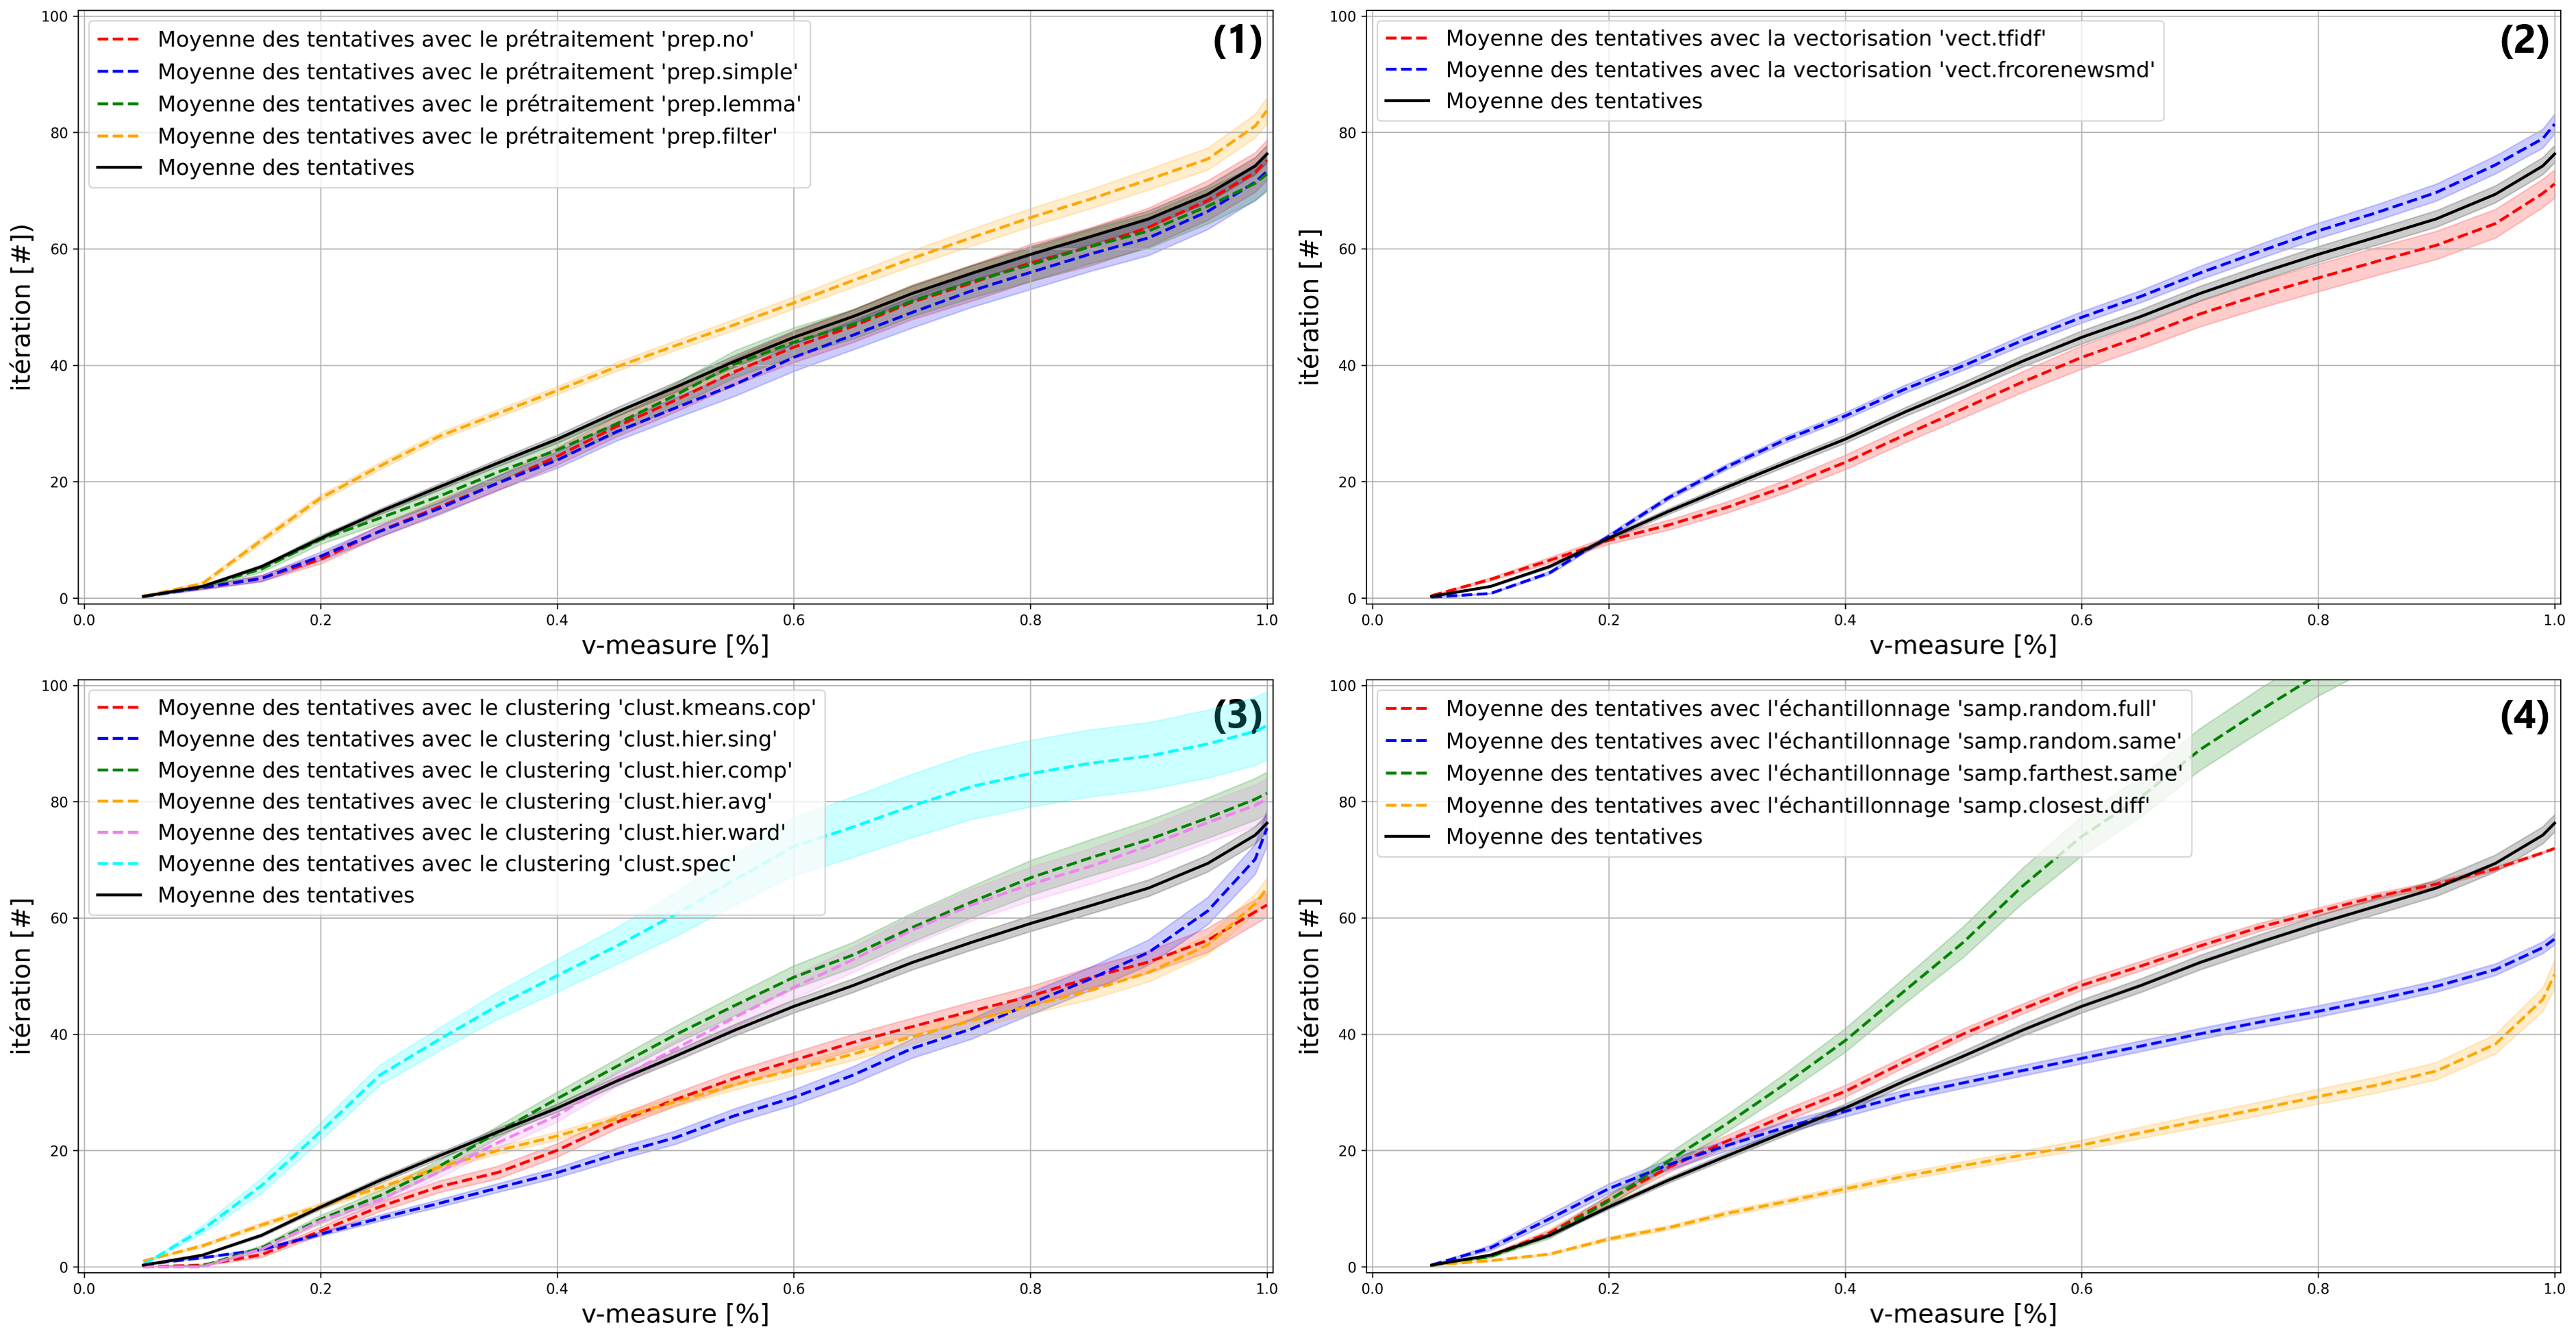
\includegraphics[width=0.95\textwidth]{figures/etude-efficience-evolution-moyenne-par-vmeasure-par-facteur}
				\caption{Évolution des moyennes du nombre d'itérations nécessaire de la méthode de \textit{clustering} interactif pour obtenir un seuil défini de \texttt{v-measure} entre un résultat obtenu et la vérité terrain, moyennes réalisées sur les différentes valeurs que peuvent prendre les facteurs analysés et affichées par facteur : \textbf{(1)} prétraitement, \textbf{(2)} vectorisation, \textbf{(3)} \textit{clustering} et \textbf{(4)} échantillonnage. \\
				Note : \textit{Le seuil d'annotation exhaustive (annoter toutes les contraintes possibles) n'étant pas exprimé en terme de \texttt{v-measure}, ce seuil n'est pas affiché ici.}}
				\label{figure:4.2.1-ETUDE-OPTIMISATION-EVOLUTION-PAR-FACTEURS}
			\end{figure}
			%
			\begin{figure}[!htb]
				\centering
				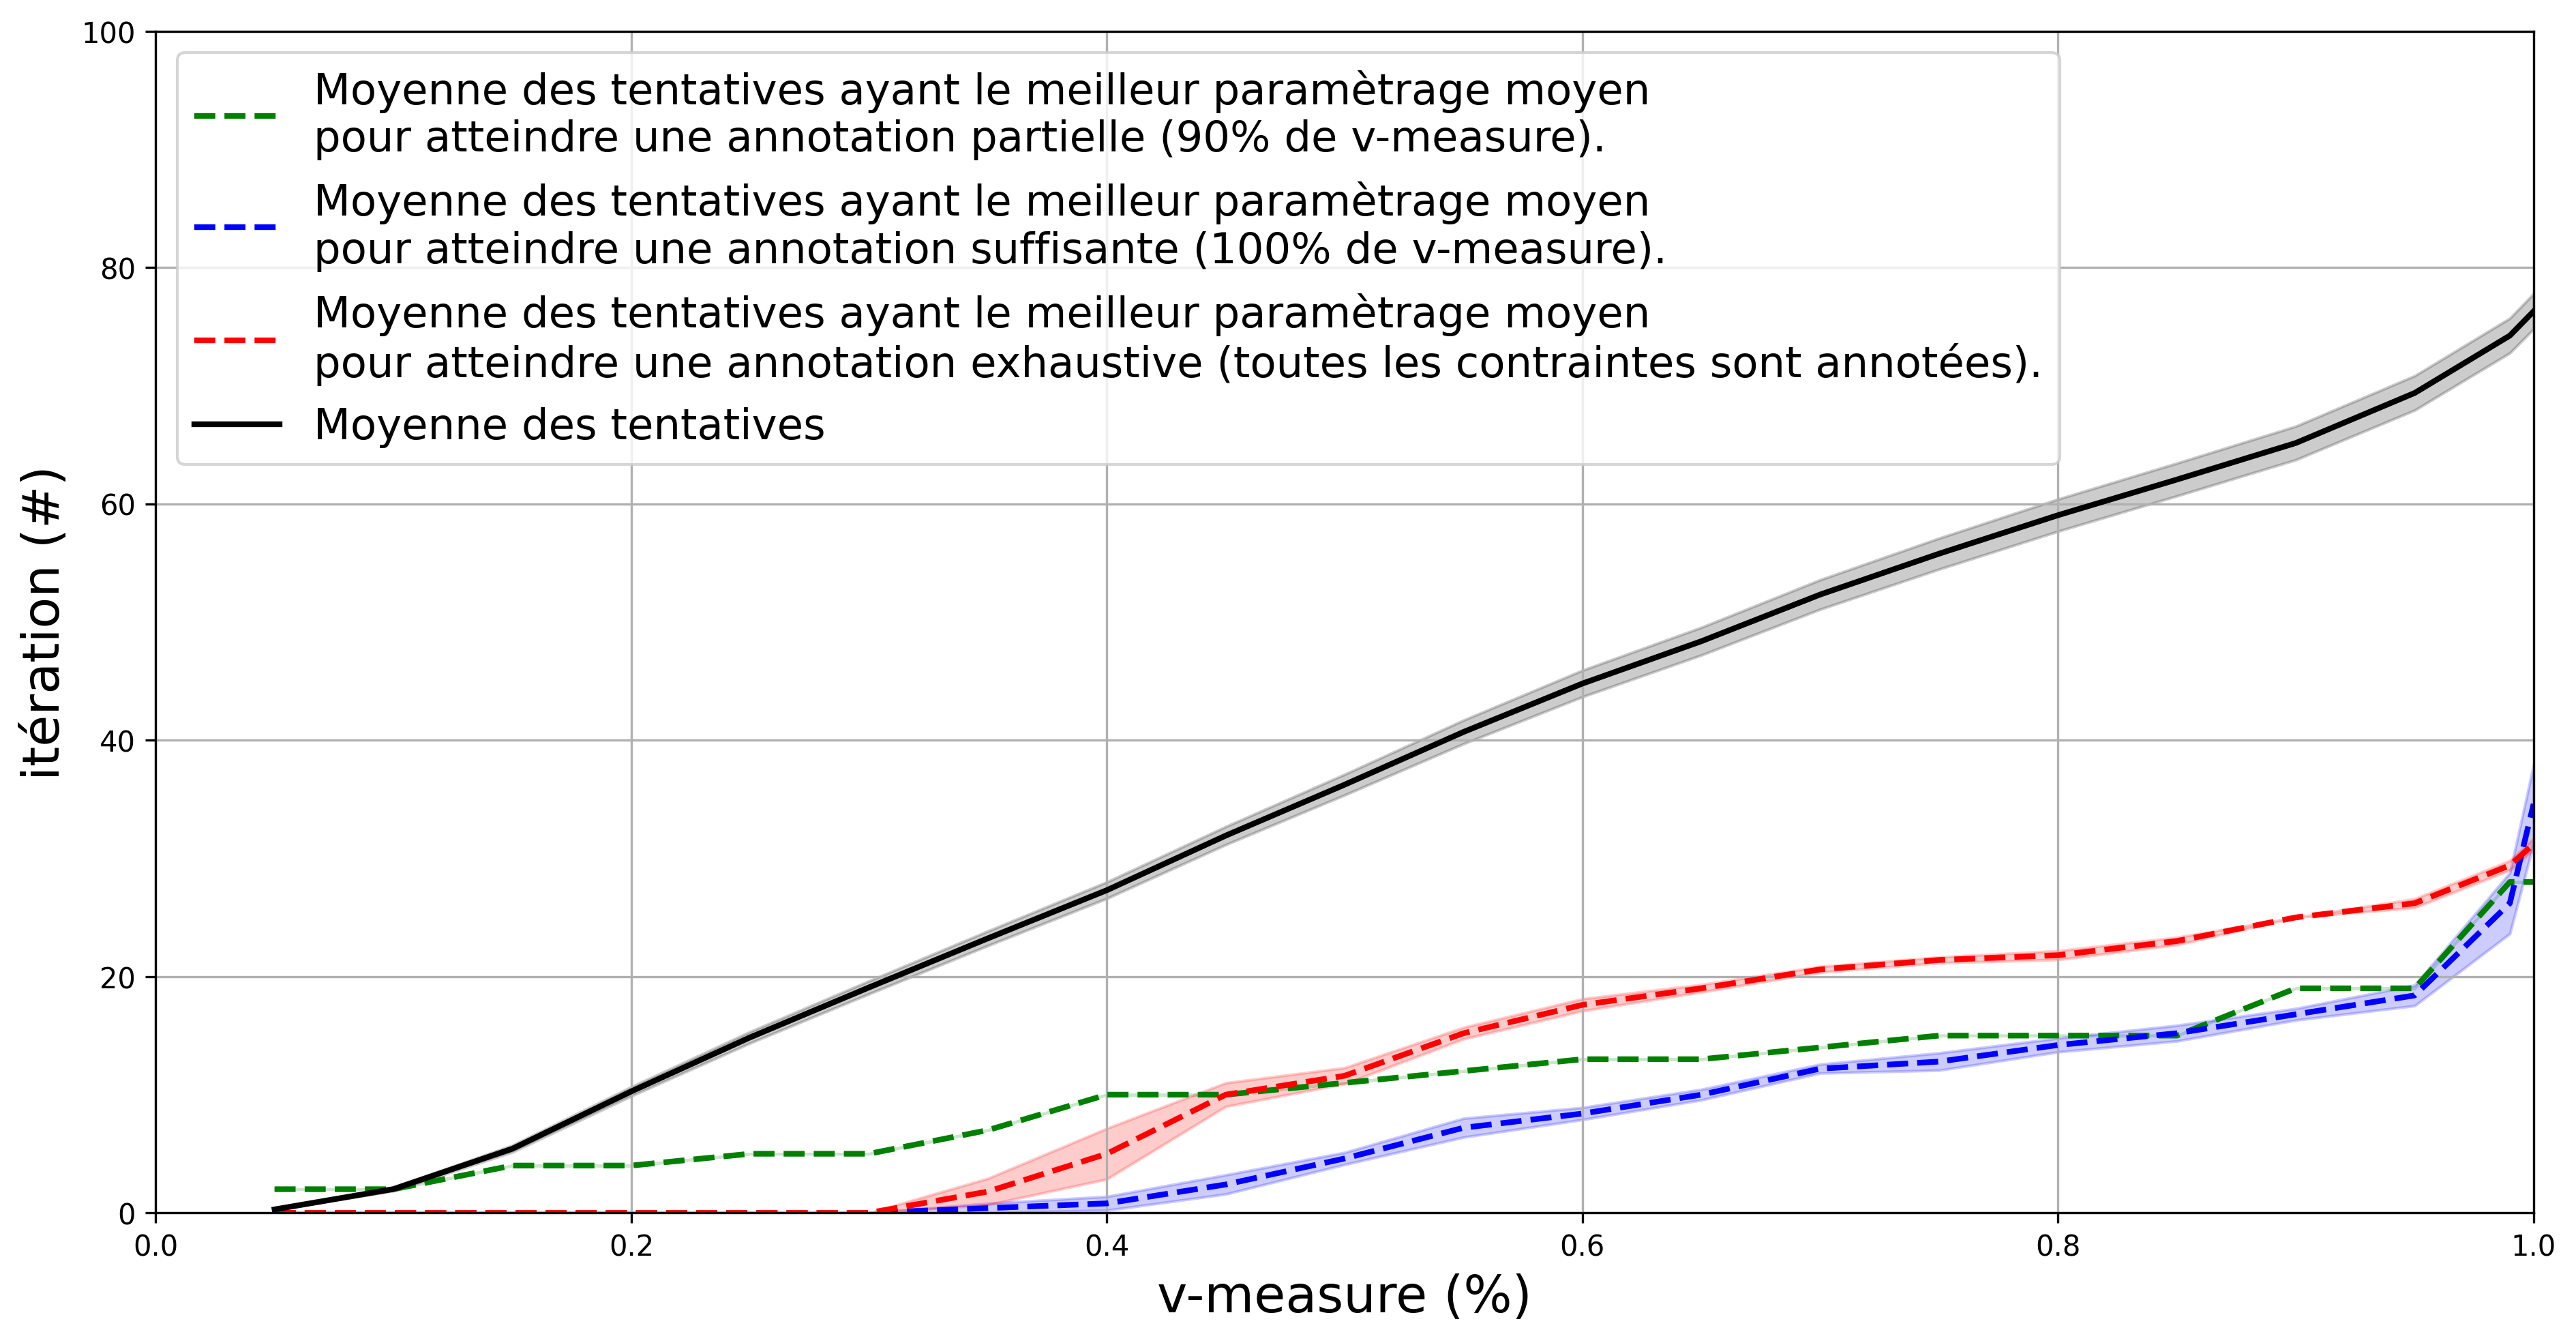
\includegraphics[width=0.95\textwidth]{figures/etude-efficience-evolution-moyenne-5best-par-vmeasure}
				\caption{Évolution des moyennes du nombre d'itérations nécessaire de la méthode de \textit{clustering} interactif pour obtenu un seuil défini de \texttt{v-measure} entre un résultat obtenu et la vérité terrain, moyennes réalisées sur les différentes seuils d'annotations étudiés : l'annotation partielle (\textit{atteindre une \texttt{v-measure} de $90$\%}), l'annotation suffisante (\textit{atteindre une \texttt{v-measure} de $100$\%}) et l'annotation exhaustive (\textit{annoter toutes les contraintes possibles}).}
				\label{figure:4.2.1-ETUDE-OPTIMISATION-EVOLUTION-MEILLEUR-PARAMETRAGE}
			\end{figure}

		%%% Discussion.
		\subsubsection{Discussion}

			% Rappel de l'objectif : être efficient.
			L'objectif de l'étude est de trouver une implémentation "efficiente" du \textit{clustering} interactif permettant d'obtenir une base d'apprentissage correctement annotée en un minimum d'annotation.
			Pour trouver si une telle implémentation existe et quels en sont les paramètres optimaux, nous avons analysé l'impact de différentes paramétrages sur les tâches principales de la méthode (\textbf{prétraitement}, \textbf{vectorisation}, \textbf{clustering sous contraintes}, \textbf{échantillonnage}) en nous basant sur des simulations d'annotation d'un jeu de données.
			
			% Première remarque : Choix d'un seuil à 90\% de v-measure.
			Dans l'optique d'être efficient, nous excluons le désir d'annoter \textbf{exhaustivement} le jeu de données car la charge de travail estimée est trop importante.
			(cf. discussion de la section~\ref{section:4.1-HYPOTHESE-EFFICACITE} (hypothèse d'efficacité))
			Nous préférons donc nous concentrer sur deux seuils d'annotation plus réalistes : celui d'une \textbf{annotation partielle} (atteindre $90$\% de \texttt{v-measure} avec la vérité terrain) et celui d'une \textbf{annotation suffisante} (atteindre $100$\% de \texttt{v-measure} avec la vérité terrain en un minimum de contraintes). 
			
			% Meilleur paramétrage.
			L'étude réalisée met en avant l'impact significatif des quatre tâches principales (\textbf{prétraitement}\todo{remarque sur la valeur de eta2}, \textbf{vectorisation}\todo{remarque sur la valeur de eta2}, \textbf{clustering sous contraintes}, \textbf{échantillonnage}) sur la vitesse de convergence de la méthode pour atteindre les seuils définis de $90$\% et $100$\% de \texttt{v-measure}. Il existe donc bien un paramétrage permettant d'optimiser l'implémentation proposée et de réduire le nombre de contraintes nécessaires à annoter :
			\begin{enumerate}
				\item pour une \textbf{annotation partielle} ($90$\% de \texttt{v-measure}), le meilleur paramétrage moyen est constitué du prétraitement simple (\texttt{prep.simple}), de la vectorisation TF-IDF (\texttt{vect.tfidf}), du \textit{clustering} hiérarchique à lien moyen (\texttt{clust.hier.avg}) et de l'échantillonnage des données les plus proches dans des clusters différents (\texttt{sampl.closest.diff}). Avec ce paramétrage, il faut en moyenne $950$ annotations de contraintes pour obtenir une \texttt{v-measure} de $90$\% ;
				\item pour une \textbf{annotation suffisante} ($100$\% de \texttt{v-measure}), le meilleur paramétrage moyen est constitué du prétraitement avec lemmatisation (\texttt{prep.lemma}), de la vectorisation TF-IDF (\texttt{vect.tfidf}), du \textit{clustering} KMeans avec modèle COP (\texttt{clust.kmeans.cop}) et de l'échantillonnage des données les plus proches dans des clusters différents (\texttt{sampl.closest.diff}). Avec ce paramétrage, il faut en moyenne $1~750$ annotations de contraintes pour obtenir une \texttt{v-measure} de $100$\% ;
				\item le cas d'une \textbf{annotation exhaustive} (annoter toutes les contraintes possibles sur les données) n'est pas explicité ici mais peut se déduire des résultats décrits plus haut.
			\end{enumerate}

			%%% Avantages.
			Ainsi, cette étude permet de répondre à la limite du nombre de contraintes requis (discutée dans l'hypothèse d'efficacité, section~\ref{section:4.1-HYPOTHESE-EFFICACITE}).
			%%% Avantage 1: Optimisation du nombre de contraintes.
			En effet, l'optimisation des paramètres de l'implémentation du \textit{clustering} interactif permet de réduire considérablement le nombre de contraintes nécessaires pour obtenir une base d'apprentissage exploitable.
			En nous basant sur le tableau~\ref{table:4.1.1-ETUDE-CONVERGENCE-EVOLUTION} de l'étude de convergence, et dans le cadre de l'annotation d'un jeu de $500$ données, nous sommes passé d'un paramétrage moyen nécessitant $3~750$ (respectivement $10~000$) contraintes à un paramétrage optimisé ne nécessitant que $950$ (respectivement $1~750$) contraintes pour atteindre un seuil de $90$\% (respectivement $100$\%) \texttt{v-measure}.
			L'ordre de grandeur de la charge de travail demandée aux annotateurs est donc située entre $2$ et $4$ fois la taille du jeu de données.
			
			% Avantage 2: La méthode devient réaliste !
			Cette estimation est plus raisonnable que celle réalisée en section~\ref{section:4.1-HYPOTHESE-EFFICACITE}.
			De plus, en considérant que les annotations sont binaires et demandent a priori une charge mental plus faible que les annotations par attribution de label ("\textit{les données sont-elles similaires ?}" vs "\textit{quel est l'étiquette de cette donnée ?}", cf. CITATION)\todo{CITATION: Development of NASA-TLX (Task Load Index): Results of Empirical and Theoretical Research}, nous pouvons espérer que la charge totale nécessaire à l'annotation avec une méthodologie basée sur le \textit{clustering} interactif est comparable à celles des méthodes traditionnelles.
			
			%%% Limites.
			Afin de compléter cette analyse d'efficience, quelques pistes sont encore à explorer.
			
			% Limite 1 : Coût temporel.
			D'une part, une étude de coût est à réaliser pour trancher le choix de paramètre optimaux réalistes.
			En effet, il est intéressant d'étudier le coût machine (temps CPU utilisé) et le coût humain (temps d'annotation) afin d'affiner les choix techniques et de compléter les arguments sur l'utilisation en situation réelle d'une méthodologie d'annotation basée sur le \textit{clustering} interactif.
			Cette étude sera l'occasion de rentrer en détail dans la comparaison de la charge demander à l'annotateur, tant sur la durée que sur la complexité de la tâche d'annotation.
			Cet aspect sera traité dans la section~\ref{section:4.3-HYPOTHESE-COUTS} (hypothèse des coûts).
			
			% Limite 2 : Valeur métier de ce 90\% (pas de vérité terrain en pratique).
			D'autre part, l'étude réalisée se base sur des seuils de performance par rapport à une vérité terrain.
			Or en situation réelle, cette comparaison avec la vérité terrain n'est pas possible car elle est précisément en cours de conception (la base d'apprentissage finale devant être la vérité terrain).
			De plus, un tel score n'est pas le plus explicite pour pour un expert métier pour qui un score de \texttt{v-measure} n'est pas révélateur de la pertinence métier de la segmentation proposée des données.
			Dans un registre similaire, il est possible que l'évolution du partitionnement des données passe par plusieurs états stables et pertinents, mais que l'annotateur soit obligé d'affiner sa vision en annotant certaines contraintes ambiguës.
			Cela peut être la cas avec des \textit{clusters} traitant en fin de compte de sujets très similaires (\textit{ajouter des \texttt{MUST-LINK} pour les fusionner}) ou avec un \textit{cluster} qui regroupe finalement plusieurs thématiques (\textit{ajouter des \texttt{CANNOT-LINK} pour le segmenter})
			Il manque donc une stratégie d'évaluation de pertinence de la base d'apprentissage en cours de construction afin d'estimer la stabilité d'un partitionnement et de la suffisance des annotations réalisées pour faire refléter la vision de l'annotateur dans le résultat obtenu.
			Cet aspect sera traité dans la section~\ref{section:4.4-HYPOTHESE-PERTINENCE} (hypothèse de pertinence).
			
			% Limite 3 : Expert métier parfait ==> simuler les erreurs.
			Pour finir, comme pour l'étude de convergence réalisé en section~\ref{section:4.1-HYPOTHESE-EFFICACITE}, nous avons supposé dans cette étude que l'annotateur est un expert métier connaissant parfaitement le domaine traité.
			Cette hypothèse forte n'est a priori pas valable en situation réelle : En effet, des erreurs d'annotations peuvent intervenir (ambiguïtés sur les données, méconnaissance du domaine, erreurs d'inattention, différence d'opinions entre annotateurs, ...), ce qui peut entraîner des divergences ou des incohérences dans la construction de la base d'apprentissage.
			Il semble donc nécessaire d'étudier les impacts de ces incohérences, ainsi que de proposer une méthode pour les prévenir ou les corriger.
			Cet aspect sera traité à la fin de ce chapitre dans la section~\ref{section:4.6-HYPOTHESE-ROBUSTESSE} (hypothèse de robustesse).
	
	
	%%%%%--------------------------------------------------------------------
	%%%%% Section 4.3: Hypothèse sur les coûts.
	%%%%%--------------------------------------------------------------------
	\newpage
	\section{Évaluation de l'hypothèse sur les coûts}
\label{section:4.3-HYPOTHESE-COUTS}

	%%%
	%%% Introduction / Transition.
	%%%
	Dans les deux sections précédentes, nous avons estimé le paramétrage du \textit{clustering} interactif le plus efficient pour atteindre $90$\% de \texttt{v-measure} avec la vérité terrain, correspondant à ce que nous appelons une annotation partielle.
	Toutefois, pour compléter l'étude de faisabilité technique de notre méthode, nous devons nous intéresser aux coûts (matériel et humain) à investir pour atteindre notre objectif.
	Nous aimerions donc vérifier l'hypothèse suivante :
	
	%%%
	%%% Formulation des hypothèses.
	%%%
	\begin{tcolorbox}[
		title=\faVial~\textbf{Hypothèse sur les coûts}~\faVial,
		colback=colorTcolorboxHypothesis!15,
		colframe=colorTcolorboxHypothesis!75,
		width=\linewidth
	]
		% Hypothèse.
		\textguillemets{\textbf{
			Il est possible d'estimer les coûts nécessaires d'une méthodologie d'annotation basée sur le \textit{clustering} interactif pour obtenir une base d'apprentissage exploitable.
			Nous étudions en particulier les coûts relatifs au temps d'annotation, au temps de calculs des algorithmes, ainsi que la durée totale de la méthode en fonction de la taille du jeu de données.
		}} \\
		
		% Figure.
		La \textsc{Figure~\ref{figure:4.3-HYPOTHESE-COUTS}} illustre cette hypothèse et l'espoir de pouvoir caractériser la qualité de la base d'apprentissage en cours de construction en fonction d'un coût temporel au lieu d'un nombre abstrait d'itérations de la méthode. 
		%
		\begin{figure}[H]  % keep [H] to be in the tcolorbox.
			\centering
			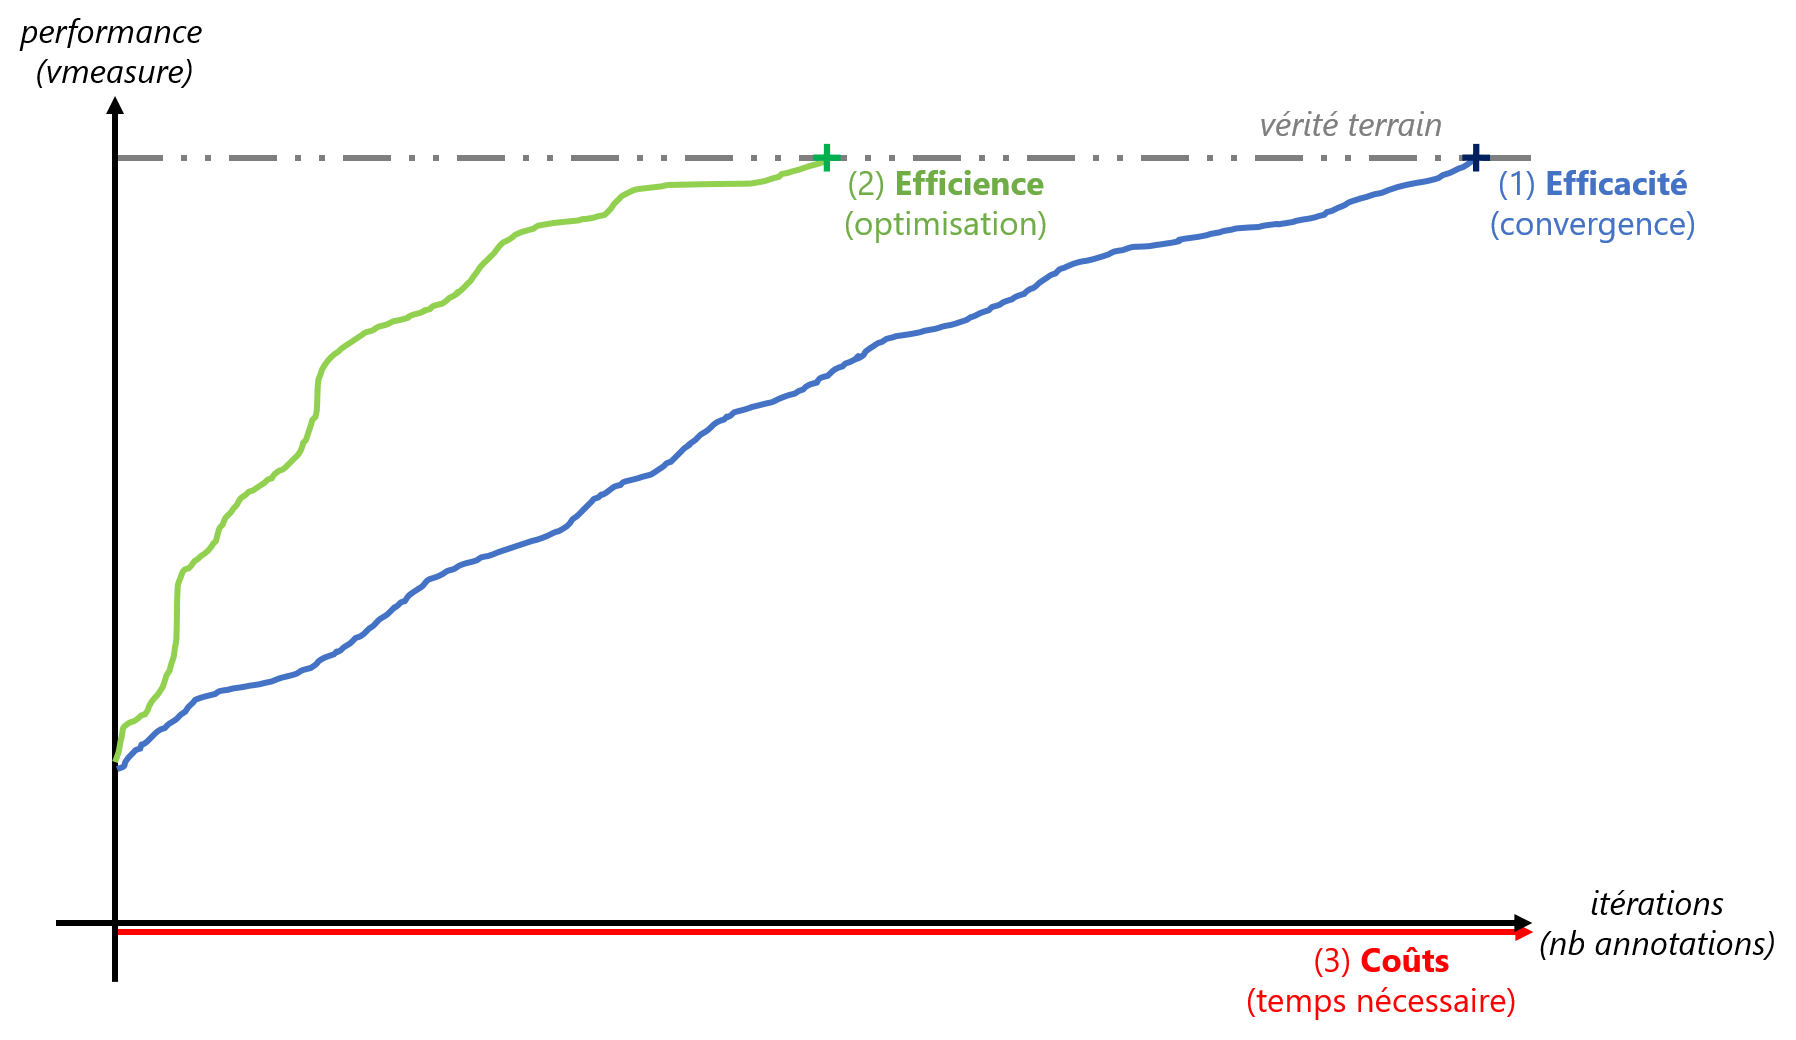
\includegraphics[width=0.95\textwidth]{figures/hypotheses-03-couts}
			\caption{
				Illustration des études réalisées sur le \textit{clustering} interactif (\textit{étape 3/6}) en schématisant l'évolution de la performance (\textit{accord avec la vérité terrain calculé en v-measure}) d'une base d'apprentissage en cours de construction en fonction du coût temporel de la méthode (\textit{temps nécessaire à l'expert métier et à la machine}).
			}
			\label{figure:4.3-HYPOTHESE-COUTS}
		\end{figure}
	\end{tcolorbox}

	% Résumé des études.
	Afin de vérifier cette hypothèse, nous organisons plusieurs expériences pour simuler et déterminer ces durées :
	\begin{itemize}
		\item une étude du \textbf{temps d'annotation} par un expert métier, mesuré lors d'une expérience d'annotation de contraintes faisant intervenir plusieurs opérateurs (cf. \textsc{Section~\ref{section:4.3.1-ETUDE-COUTS-TEMPS-ANNOTATION}}) ;
		\item une étude du \textbf{temps de calcul} des algorithmes, modélisé en exécutant les différentes implémentations du \textit{clustering} interactif avec diverses valeurs d'arguments (cf. \textsc{Section~\ref{section:4.3.2-ETUDE-COUTS-TEMPS-CALCUL}}) ;
		\item et une étude du \textbf{nombre de contraintes} nécessaires en fonction du nombre de données à traiter, estimé en simulant la création d'une base d'annotation avec notre méthodologie sur des jeux de données de différentes tailles (cf. \textsc{Section~\ref{section:4.3.3-ETUDE-COUT-NOMBRE-CONTRAINTES}}).
	\end{itemize}
	Nous exposons nos conclusions sur l'estimation du \textbf{temps total} à investir et réalisons une comparaison avec une organisation plus traditionnelle d'un projet d'annotation en \textsc{Section~\ref{section:4.3.4-ETUDE-COUTS-TOTAL}}.
	
	
	%%%
	%%% Subsection 4.3.1: Étude du temps d'annotation nécessaire pour traiter un lot de contraintes en chronométrant des opérateurs en situation réelle
	%%%
	\subsection{Étude du temps d'annotation nécessaire pour traiter un lot de contraintes en chronométrant des opérateurs en situation réelle}
	\label{section:4.3.1-ETUDE-COUTS-TEMPS-ANNOTATION}
		
		% Objectif de l'expérience.
		Nous voulons estimer le temps nécessaire à un opérateur pour annoter un lot de contraintes.
		Pour cela, nous allons chronométrer plusieurs experts métiers en train d'annoter un même échantillon et modéliser le nombre de contraintes par minute, ainsi que son évolution au cours de plusieurs sessions d'annotation.
		De plus, nous aimerions aussi confirmer que l'ajout de contraintes dans notre contexte s'apparente à une tâche "intuitive", c'est-à-dire que l'annotation se fait dans la réaction et non dans la réflexion (voir \cite{kahneman:2011:thinking-fast-slow} qui distingue un \textit{système 1} intuitif, rapide, de l'ordre de l'émotion, et un \textit{système 2} plus lent, logique et réfléchi).
		Pour ce faire, nous estimons grossièrement le temps nécessaire à l'annotation réactive d'une contrainte, nous le comparons au temps moyen estimé lors de notre expérience, et nous nous demandons si la différence observée peut cacher un mécanisme cognitif plus complexe.
	
		%%% Protocole expérimental.
		\subsubsection{Protocole expérimental}
			
			% Axiome.
			\begin{leftBarWarning}
				Dans cette étude, nous supposons que les annotateurs de l'expérience connaissent parfaitement le domaine traité dans le jeu de données, et qu'ils sont capables de caractériser sans ambiguïté la similitude entre deux données issues de cet ensemble.
				Afin de pourvoir faire cette hypothèse forte, et ainsi limiter les bruits dans l'analyse des résultats, le jeu de données devra traiter d'un sujet de culture générale (ne nécessitant donc pas de connaissance particulière) et des réviseurs supprimeront en amont et d'un commun accord les données trop spécifiques ou trop ambiguës.
			\end{leftBarWarning}
			
			% Pseudo-code.
			Pour résumer le protocole expérimental que nous décrivons ci-dessous, vous pouvez vous référer au pseudo-code décrit dans \textsc{Algorithme~\ref{algorithm:4.3.1-ETUDE-COUTS-TEMPS-ANNOTATION-PROTOCOLE}}.

			\begin{algorithm}
				\KwData{jeu de données annotées (vérité terrain)}
				\KwIn{plusieurs réviseurs, plusieurs annotateurs}
				%
				\textbf{initialisation}: définir et revoir le jeu de données entre réviseurs \;
				\textbf{échantillonnage}: sélectionner une base de contraintes avec \texttt{samp.rand.full} \;
				\textbf{temps théorique}: estimation du temps nécessaire à l'annotation d'une contrainte \;
				\ForEach{annotateur}{
					 \While{la base de contraintes n'a pas été entièrement annotée}{
						\textbf{chronomètre}: \textbf{START} \;
						\textbf{annotation}: annoter une partie des contraintes \;
						\textbf{revue}: revue des contraintes en conflits d'annotation \;
						\textbf{chronomètre}: \textbf{STOP} \;
						\textbf{mesure}: estimer la différence de chronomètre pour cette session \;
					}
				}
				\textbf{analyse}: modéliser le temps d'annotation d'un lot de contraintes \;
				%
				\KwResult{modélisation du temps d'annotation d'un lot de contraintes}
				%
				\caption{\textit{
					Description en pseudo-code du protocole expérimental de l'étude du temps d'annotation d'un lot de contraintes par plusieurs experts métiers en situation réelle.
				}}
				\label{algorithm:4.3.1-ETUDE-COUTS-TEMPS-ANNOTATION-PROTOCOLE}
			\end{algorithm}
			
			% Détails de l'expérience : préparation du jeu de données.
			Nous allons procéder en plusieurs étapes.
			D'abord, il faut choisir un jeu de données approprié : pour valider notre hypothèse forte sur les compétences de nos annotateurs, nous cherchons un jeu de données traitant d'un sujet de culture général.
			Pour cette expérience, nous avons donc choisi \texttt{MLSUM} : une collecte d'articles de journaux, classés par catégorie de publication et décrits par leur titre et leur résumé.
			Nous nous intéressons ici à la tâche de classification d'un titre d'article en fonction de sa catégorie de publication.
			Comme certains titres peuvent porter à confusion (un titre d'article n'étant pas toujours explicite sur son contenu), deux réviseurs sont chargés de choisir les données les plus explicites sur un échantillon d'un millier de données représentatives des catégories les plus communes.
			L'échantillon résultant, noté \texttt{MLSUM FR Train Subset (v1.0.0-schild)}, est composé de $744$ titres d'articles rédigés en français et répartis en $14$ classes (\textit{économie}, \textit{sport}, ...).
			Pour plus de détails, consultez l'annexe~\ref{annex:A.2-DATASET-MLSUM-SUBSET-SCHILD}.
			
			% Détails de l'expérience : sélection des contraintes à annoter.
			À partir de ces données, nous sélectionnons un lot de $1~000$ contraintes à annoter.
			Comme nous nous intéressons exclusivement au temps d'annotation pour cette expérience (et que nous ne regardons pas le nombre d'itérations de la méthode), nous utilisons l'échantillonnage purement aléatoire (\texttt{samp.rand.full}).
			L'analyse de l'accord inter-annotateurs sera réalisé en \textsc{Section~\ref{section:4.6.3-ETUDE-ROBUSTESSE-SCORE-INTER-ANNOTATEURS}}.
			
			% Détails de l'expérience : estimation du temps théorique nécessaire à l'annotation d'une contrainte.
			Sur la base de cette échantillon, nous pouvons approximer le temps théorique nécessaire à l'annotation d'une contrainte à $6.8$ secondes.
			En effet, il faut d'abord considérer la taille moyenne des titres d'article à lire et en déduire le temps dédié à la lecture des deux textes de la contraintes.
			En utilisant l'approximation d'une lecture silencieuse par un adulte à $238$ mots par minute (\cite{brysbaert:2019:how-many-words}) et en mesurant la taille moyenne des titre d'article à $10.1$ mots, on en déduit que le temps de lecture d'un texte est environ de $2.55$ secondes.
			Ensuite, il convient d'intégrer la durée de traitement cognitif requis pour estimer si les deux phrases sont similaires ou discordantes.
			À cet effet, nous retenons $1$ seconde\footnote{
				Nous pourrions faire le parallèle avec la composante \texttt{P600} communément admise en neuroscience pour caractériser la réaction provoquée par la dissonance grammaticale ou syntaxique d'une phrase.
				Nous arrondissons à $1$ seconde pour garder une marge d'erreur.
			} (\cite{purves-brannon:2013:principles-cognitive-neuroscience})
			en admettant que cette tâche est rapide.
			Enfin, nous ajoutons $1$ seconde supplémentaire pour représenter la réaction motrice (clic de bouton) et le délais applicatif (rechargement de la page).
			Au total, nous obtenons ainsi un temps d'annotation moyen de $7$ secondes.
			Bien entendu, cette durée reste approximative, mais elle nous permet de discuter de l'ordre de grandeur à manipuler durant l'annotation.
			
			% Détails de l'expérience : annotations et consignes.
			Ensuite, un groupe de $14$ annotateurs vont annoter la sélection de $1~000$ contraintes en plusieurs sessions.
			Les directives données aux opérateurs sont les suivantes:
			\begin{itemize}
				\item \textbf{Contexte de l'opérateur} :
				\textguillemets{\textit{Vous êtes des \textbf{experts de la presse et de l'actualité} ; Vous voulez classer des articles dans des catégories en fonction de leur titre ; Vous ne savez pas précisément quelles catégories vous allez utiliser pour classer vos articles ; Mais vous savez \textbf{caractériser la similitude} de deux articles}} ;
				\item \textbf{Contexte sur le jeu de données} :
				\textguillemets{\textit{Le thème sont les catégories d'articles de presse ; La vérité terrain contient entre $10$ et $20$ catégories parmi les plus communes de la presse ; La vérité terrain contient entre $30$ et $100$ articles par catégorie ; Vous \textbf{pouvez regarder le jeu de données non annoté} autant que vous le voulez (disponible dans l'onglet \texttt{TEXTS} de l'application)}} ;
				\item \textbf{Objectif de l'expérience} :
				\textguillemets{\textit{Je veux savoir le temps nécessaire pour annoter un certain nombre de contraintes ; Autrement dit : \textbf{Pour annoter 1000 contraintes, combien de temps me faut-il ?}}} ;
				\item \textbf{Consignes d'annotations} :
				\textguillemets{\textit{Faites des séries de \textbf{15 minutes minimum} pour avoir de la régularité ; Si possible, \textbf{isolez-vous} pour ne pas être dérangé et ne pas fausser les résultats ; Pour chaque série, \textbf{notez le temps et le nombre de contraintes annotés} ; Si vous ne savez pas quoi annoter (trop ambigu, vocabulaire inconnu, ...), \textbf{passez au suivant sans annoter} (vous êtes sensés être des experts de la presse !)}}.
			\end{itemize}
			%
			Pour réaliser l'annotation, les opérateurs auront accès à l'application web développée au cours de ce doctorat.
			Des captures d'écran sont disponibles en \textsc{Figure~\ref{figure:4.3.1-ETUDE-COUTS-TEMPS-ANNOTATION-APPLICATION-ANNOTATION}} et \textsc{Figure~\ref{figure:4.3.1-ETUDE-COUTS-TEMPS-ANNOTATION-APPLICATION-LISTE-CONTRAINTES}}.
			Une description plus détaillée de l'application et de ses fonctionnalités est disponible en \textsc{Section~\ref{section:3.3-DESCRIPTION-IMPLEMENTATION}}\todo{description à faire}.
			%
			\begin{figure}[!htb]
				\centering
				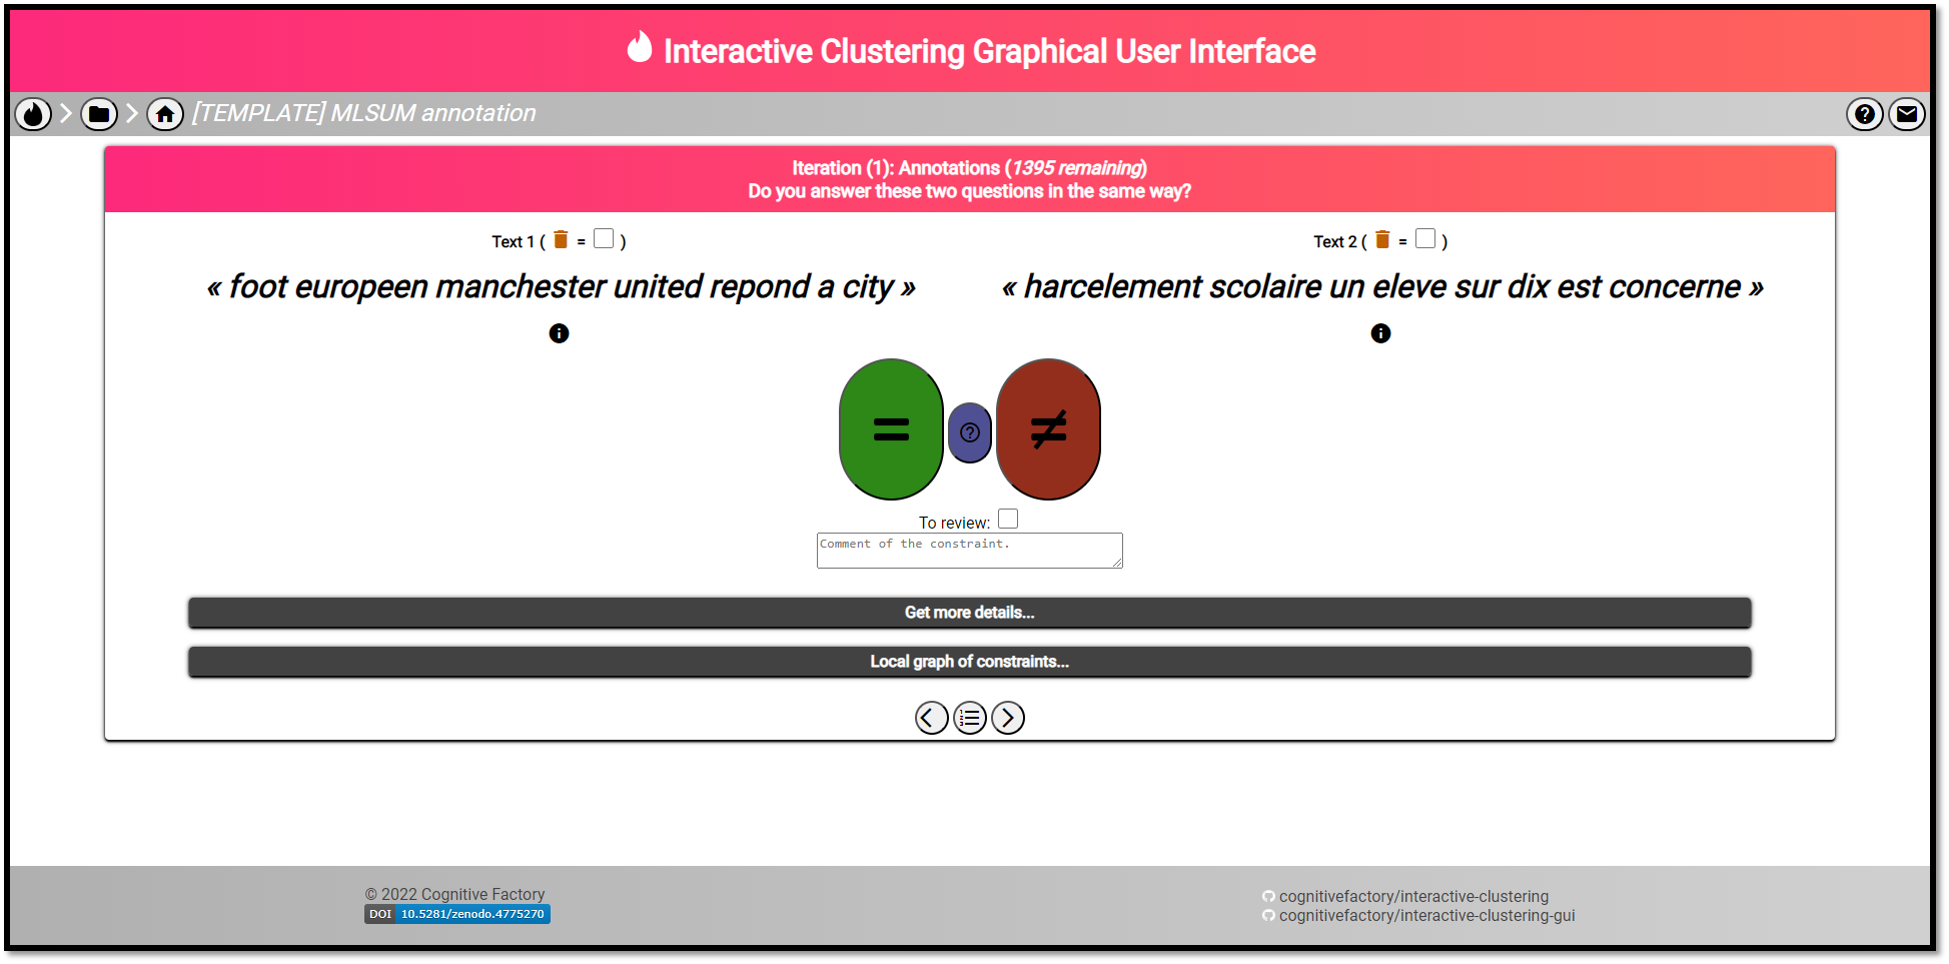
\includegraphics[width=0.95\textwidth]{figures/etude-temps-annotation-0application-annotation}
				\caption{
					Capture d'écran de l'application web permettant utilisant notre méthodologie de \textit{clustering} interactif pour annoter des contraintes (page d'annotation). Les deux textes à annoter sont disposés à gauche et droite de l'écran. Chacun dispose d'un cache à cocher si le texte n'est pas pertinent à analyser (\textit{ambigu, hors périmètre, incompréhensible, ...}).\\
					Les boutons à disposition permettent respectivement d'annoter un \texttt{MUST-LINK} si les données sont similaires (\textit{bouton en vert}), un \texttt{CANNOT-LINK} si les données ne sont pas similaire (\textit{bouton en rouge}), d'ignorer la contrainte pour laisser la main à l'algorithme de \textit{clustering} (\textit{bouton en bleu}), et d'ajouter un commentaire pour revoir la contrainte plus tard (\textit{case à choser et champ de texte libre}). Deux éléments déroulant permettent d'avoir des informations supplémentaires (\textit{metadata de sélection et de \textit{clustering}, représentation graphique des liens entre contraintes annotées}). Les boutons de navigation (\textit{boutons flèches et liste}) sont disponibles en bas de page.
				}
				\label{figure:4.3.1-ETUDE-COUTS-TEMPS-ANNOTATION-APPLICATION-ANNOTATION}
			\end{figure}
			\begin{figure}[!htb]
				\centering
				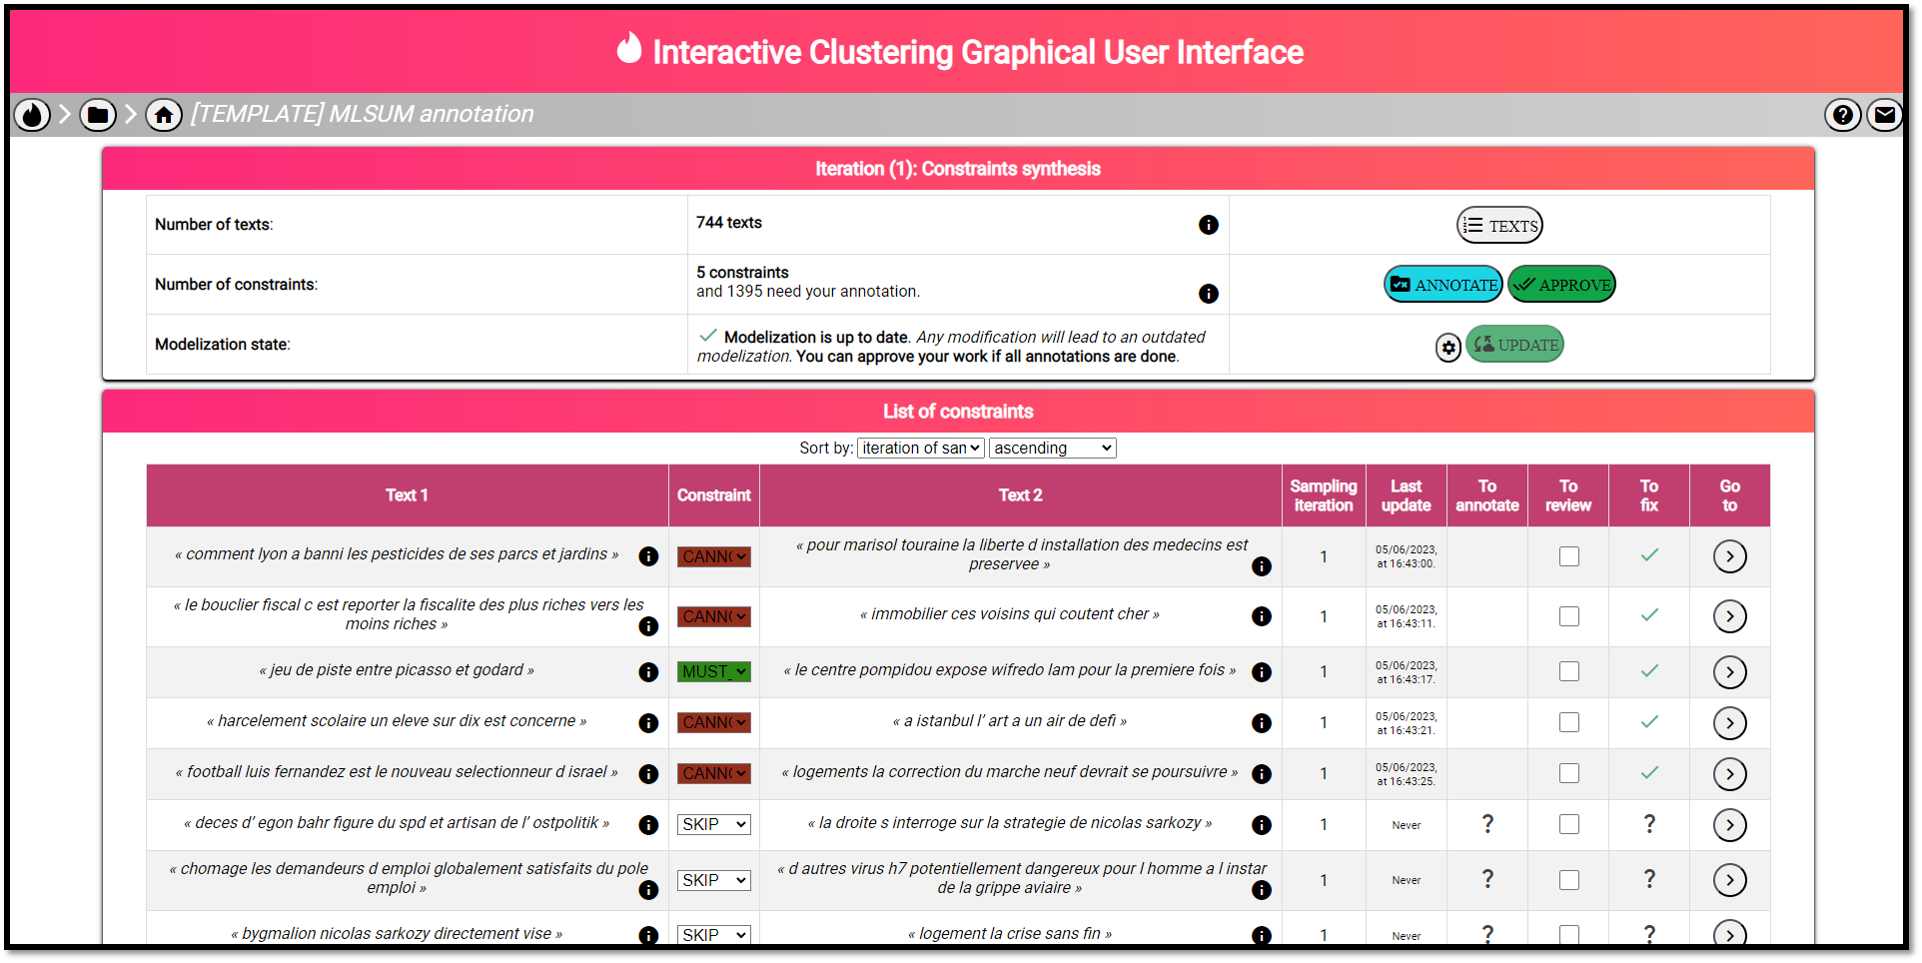
\includegraphics[width=0.95\textwidth]{figures/etude-temps-annotation-0application-liste-contraintes}
				\caption{
					Capture d'écran de l'application web permettant utilisant notre méthodologie de \textit{clustering} interactif pour annoter des contraintes (page d'inventaire des contraintes à annoter).\\
					La partie supérieure permet d'identifier le nombre de textes et de contraintes sur le projet, ainsi que les boutons destinés à calculer les transitivités entre les contraintes et à approuver le travail réalisé si aucune transitivité n'entre en conflit avec un contrainte annotée. La partie inférieure liste l'ensemble des contraintes du projet, avec les annotations réalisées, l'itération à laquelle la contraintes a été sélectionnée et annotée, si elle est à revoir ou si une incohérence la concernant est détectée.
				}
				\label{figure:4.3.1-ETUDE-COUTS-TEMPS-ANNOTATION-APPLICATION-LISTE-CONTRAINTES}
			\end{figure}
			
			
			% Détails de l'expérience : modélisation.
			Une fois les sessions d'annotations terminées, nous entraînons un modèle linéaire généralisé (\textit{GLM}) pour estimer le temps d'annotation moyen pour un lot de contraintes (dont la taille est notée $\texttt{batch\_size}$).
			Ce modèle sera caractérisé par le coefficient de détermination généralisé \texttt{R²} de \textit{Cox et Snel} (\cite{diamond-etal:1990:analysis-binary-data}), la log-vraisemblance \texttt{llf} (\cite{edwards:1992:likelihood}) et la log-vraisemblance \texttt{llf\_null} du modèle \textit{null}.
			Nous discutons aussi de l'évolution de la vitesse d'un opérateur au cours des différentes sessions d'annotation.

			% Référence scripts.
			\begin{leftBarInformation}
				L'outil d'annotation utilisé est accessible dans~\cite{schild-etal:2022:cognitivefactory-interactiveclusteringgui}.
				Les scripts de l'expérience, réalisés avec des \textit{notebooks} Python (\cite{van-rossum-drake:2009:python-reference-manual}), ainsi que le projet à importer dans l'outil d'annotation, sont disponibles dans un dossier dédié de~\cite{schild:2021:cognitivefactory-interactiveclusteringcomparativestudy}.
				Nous utilisons entre autres les librairies \texttt{datetime} et \texttt{statsmodels} (\cite{seabold-perktold:2010:statsmodels-econometric-statistical}).
			\end{leftBarInformation}

		%%% Résultats.
		\subsubsection{Résultats obtenus}
		
			% Taux de participation.
			Durant cette expérience, $14$ annotateurs ont participé à l'annotation de $1~000$ contraintes aléatoires sur un jeu de données.
			Par manque de disponibilités, $4$ annotateurs n'ont que partiellement réalisé leur tâche : nous avons toutefois intégré leurs participations car elles contenaient toutes au moins $150$ annotations.
			
			% Statistiques descriptives.
			D'après les observations, un annotateur réalisait en moyenne $170.7$ contraintes par session d'annotation (min: $43$, max: $547$, médiane: $138$, écart-type: $106.4$) ce qui lui demandait en moyenne $23.1$ minutes (min: $3.0$, max: $92.0$, écart-type: $14.4$).
			De plus, la vitesse d'annotation moyenne était de $7.7$ contraintes par minute (min: $3.5$, max: $14.3$, écart-type: $2.9$).
			
			% Modélisation du temps d'annotation.
			Le modèle linéaire généralisé entraîné sur les mesures de temps d'annotations (\texttt{R²}: $0.910$, \texttt{llf}: $-499.15$, \texttt{llf\_null}: $-539.95$) nous permet de déduire l'équation suivante :
			%
			\begin{equation}
				\label{equation:4.3.1-ETUDE-COUT-COUTS-TEMPS-ANNOTATION}
				\texttt{annotation\_time}~[s]~
				\propto~7.8 \cdot \texttt{batch\_size}
			\end{equation}
		
			% Affichage du temps d'annotation.
			La \textsc{Figure~\ref{figure:4.3.1-ETUDE-COUTS-TEMPS-ANNOTATION-SIMULATION}} représente cette modélisation du temps d'annotation en comparaison avec les mesures réalisées lors de l'expérience.
			Pour rappel, le temps théorique estimé précédemment est de $7$ secondes par contrainte.
			%
			\begin{figure}[!htb]
				\centering
				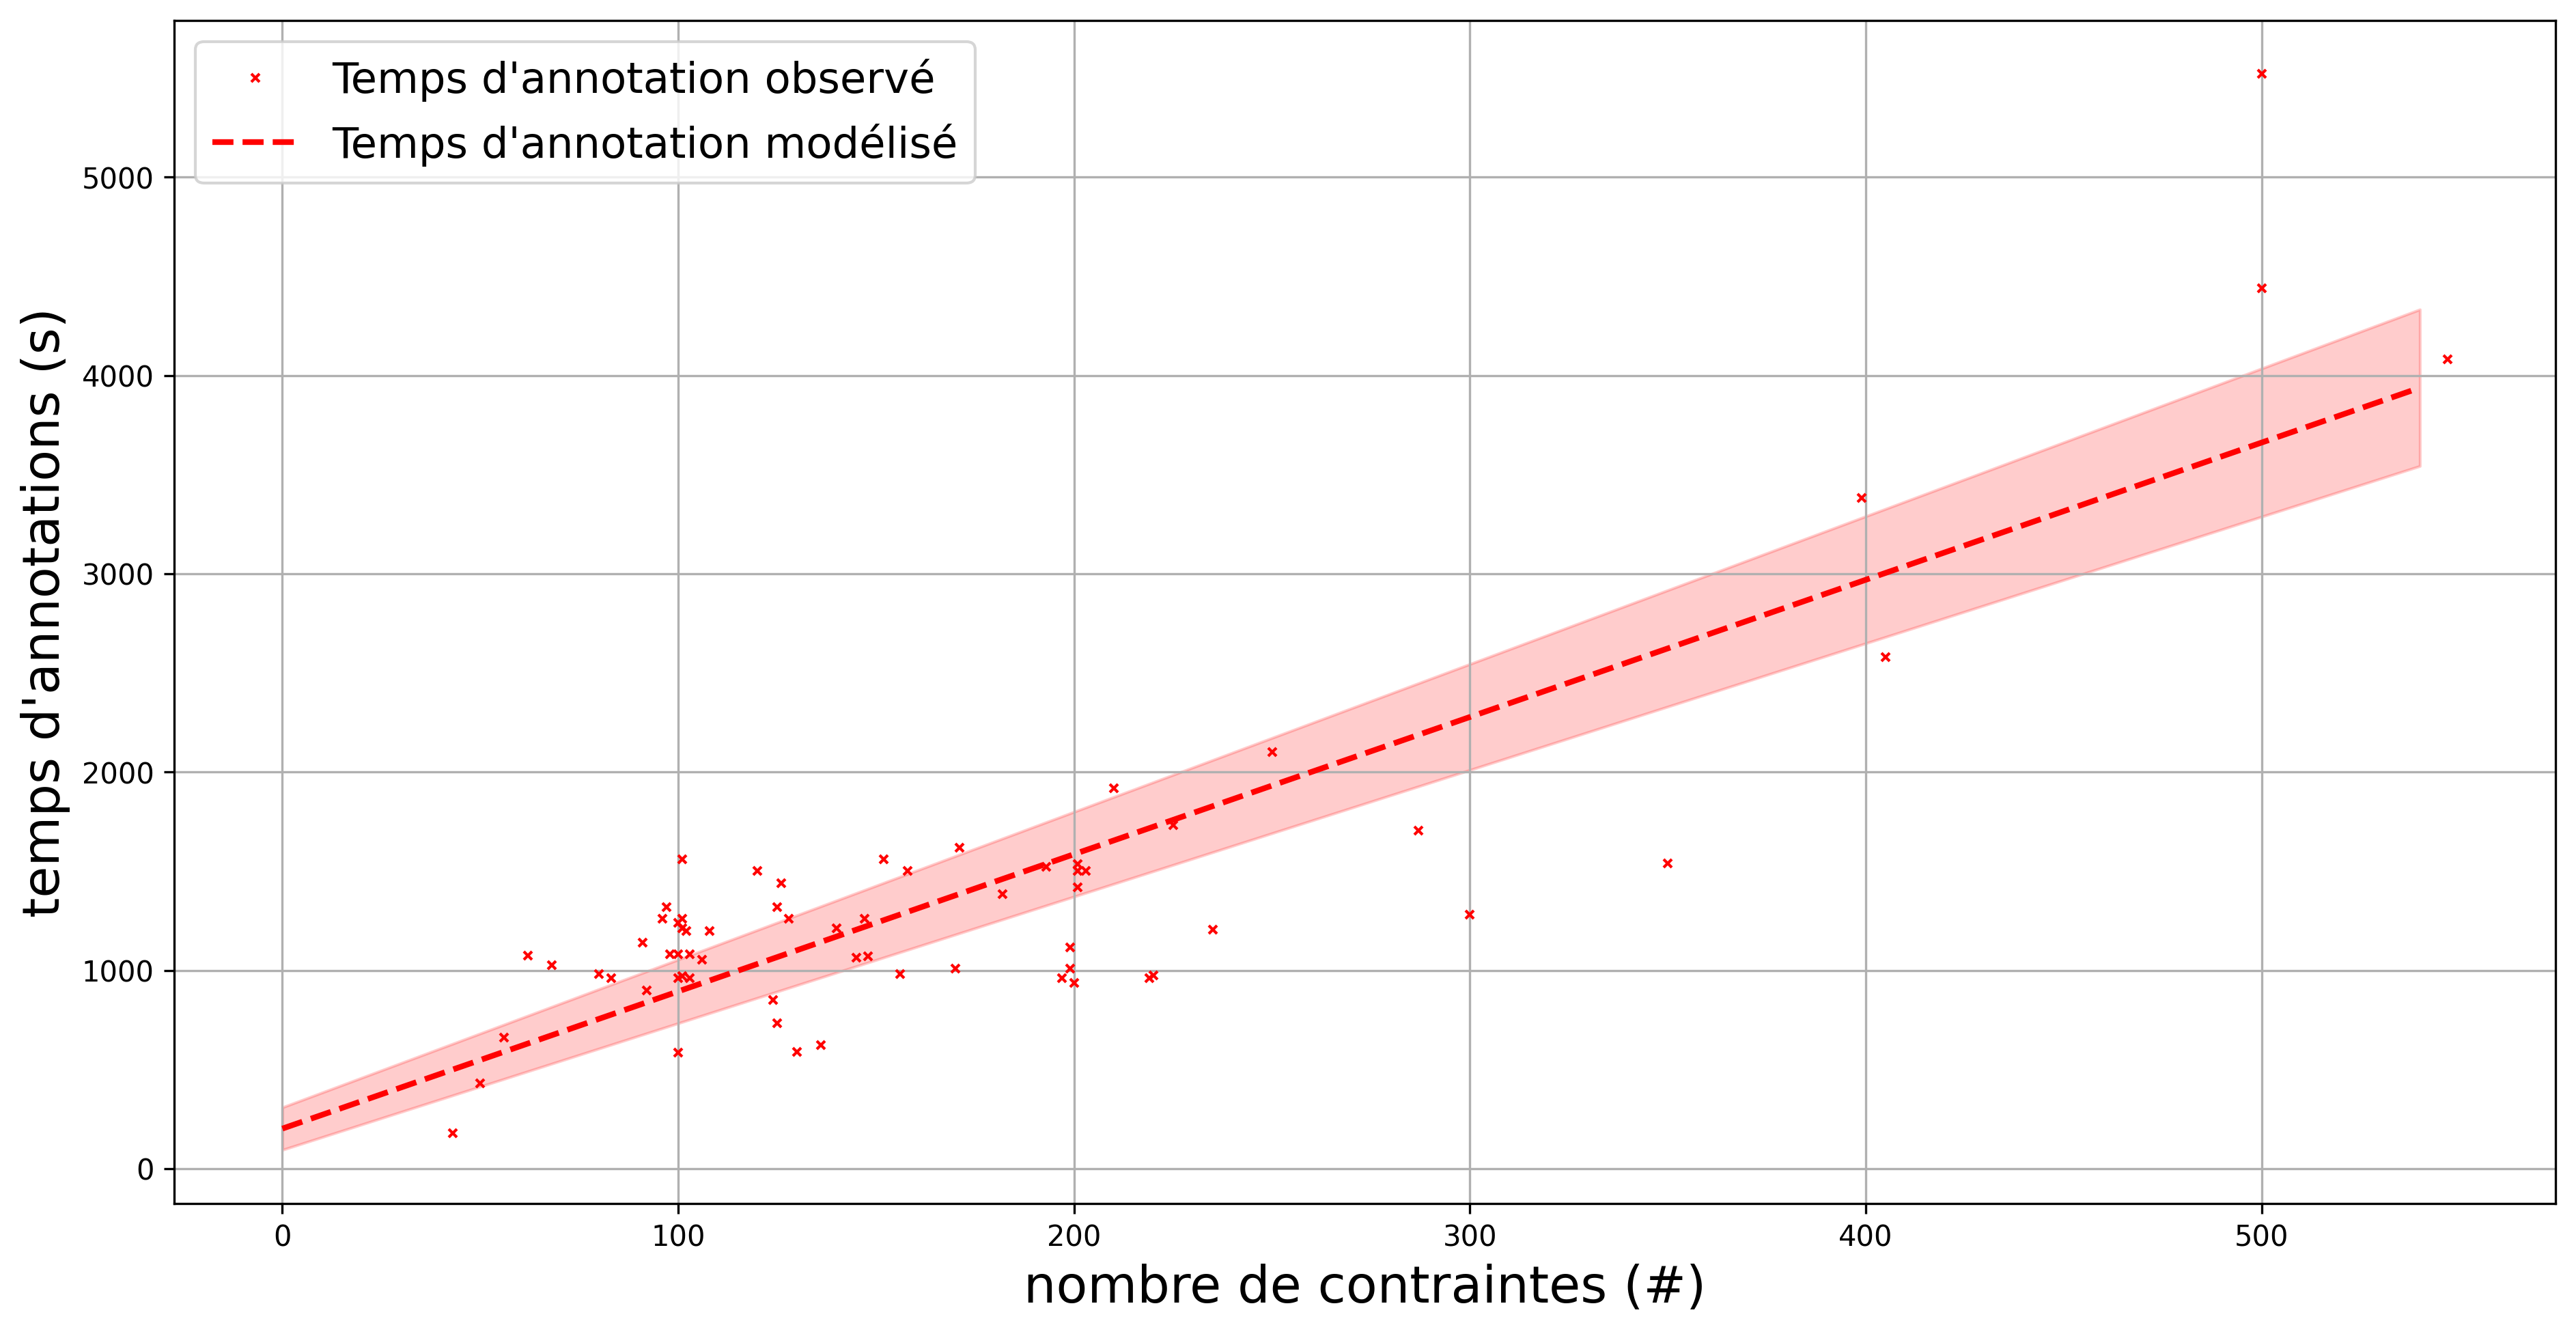
\includegraphics[width=0.95\textwidth]{figures/etude-temps-annotation-1-modelisation-temps}
				\caption{
					Estimation du temps nécessaire (en minutes) pour annoter un lot de contraintes.
				}
				\label{figure:4.3.1-ETUDE-COUTS-TEMPS-ANNOTATION-SIMULATION}
			\end{figure}
		
			% Étude de cas.
			En ce qui concerne l'évolution de la vitesse d'annotation au cours des sessions, aucune tendance significative n'a été identifiée. 
			La \textsc{Figure~\ref{figure:4.3.1-ETUDE-COUTS-TEMPS-ANNOTATION-EXEMPLE}} représente l'évolution de vitesse d'annotation pour quatre opérateurs (les deux plus rapides et les deux plus lents).
			Ces données sont l'objet d'une étude de cas dans la discussion ci-dessous.
			%
			\begin{figure}[!htb]
				\centering
				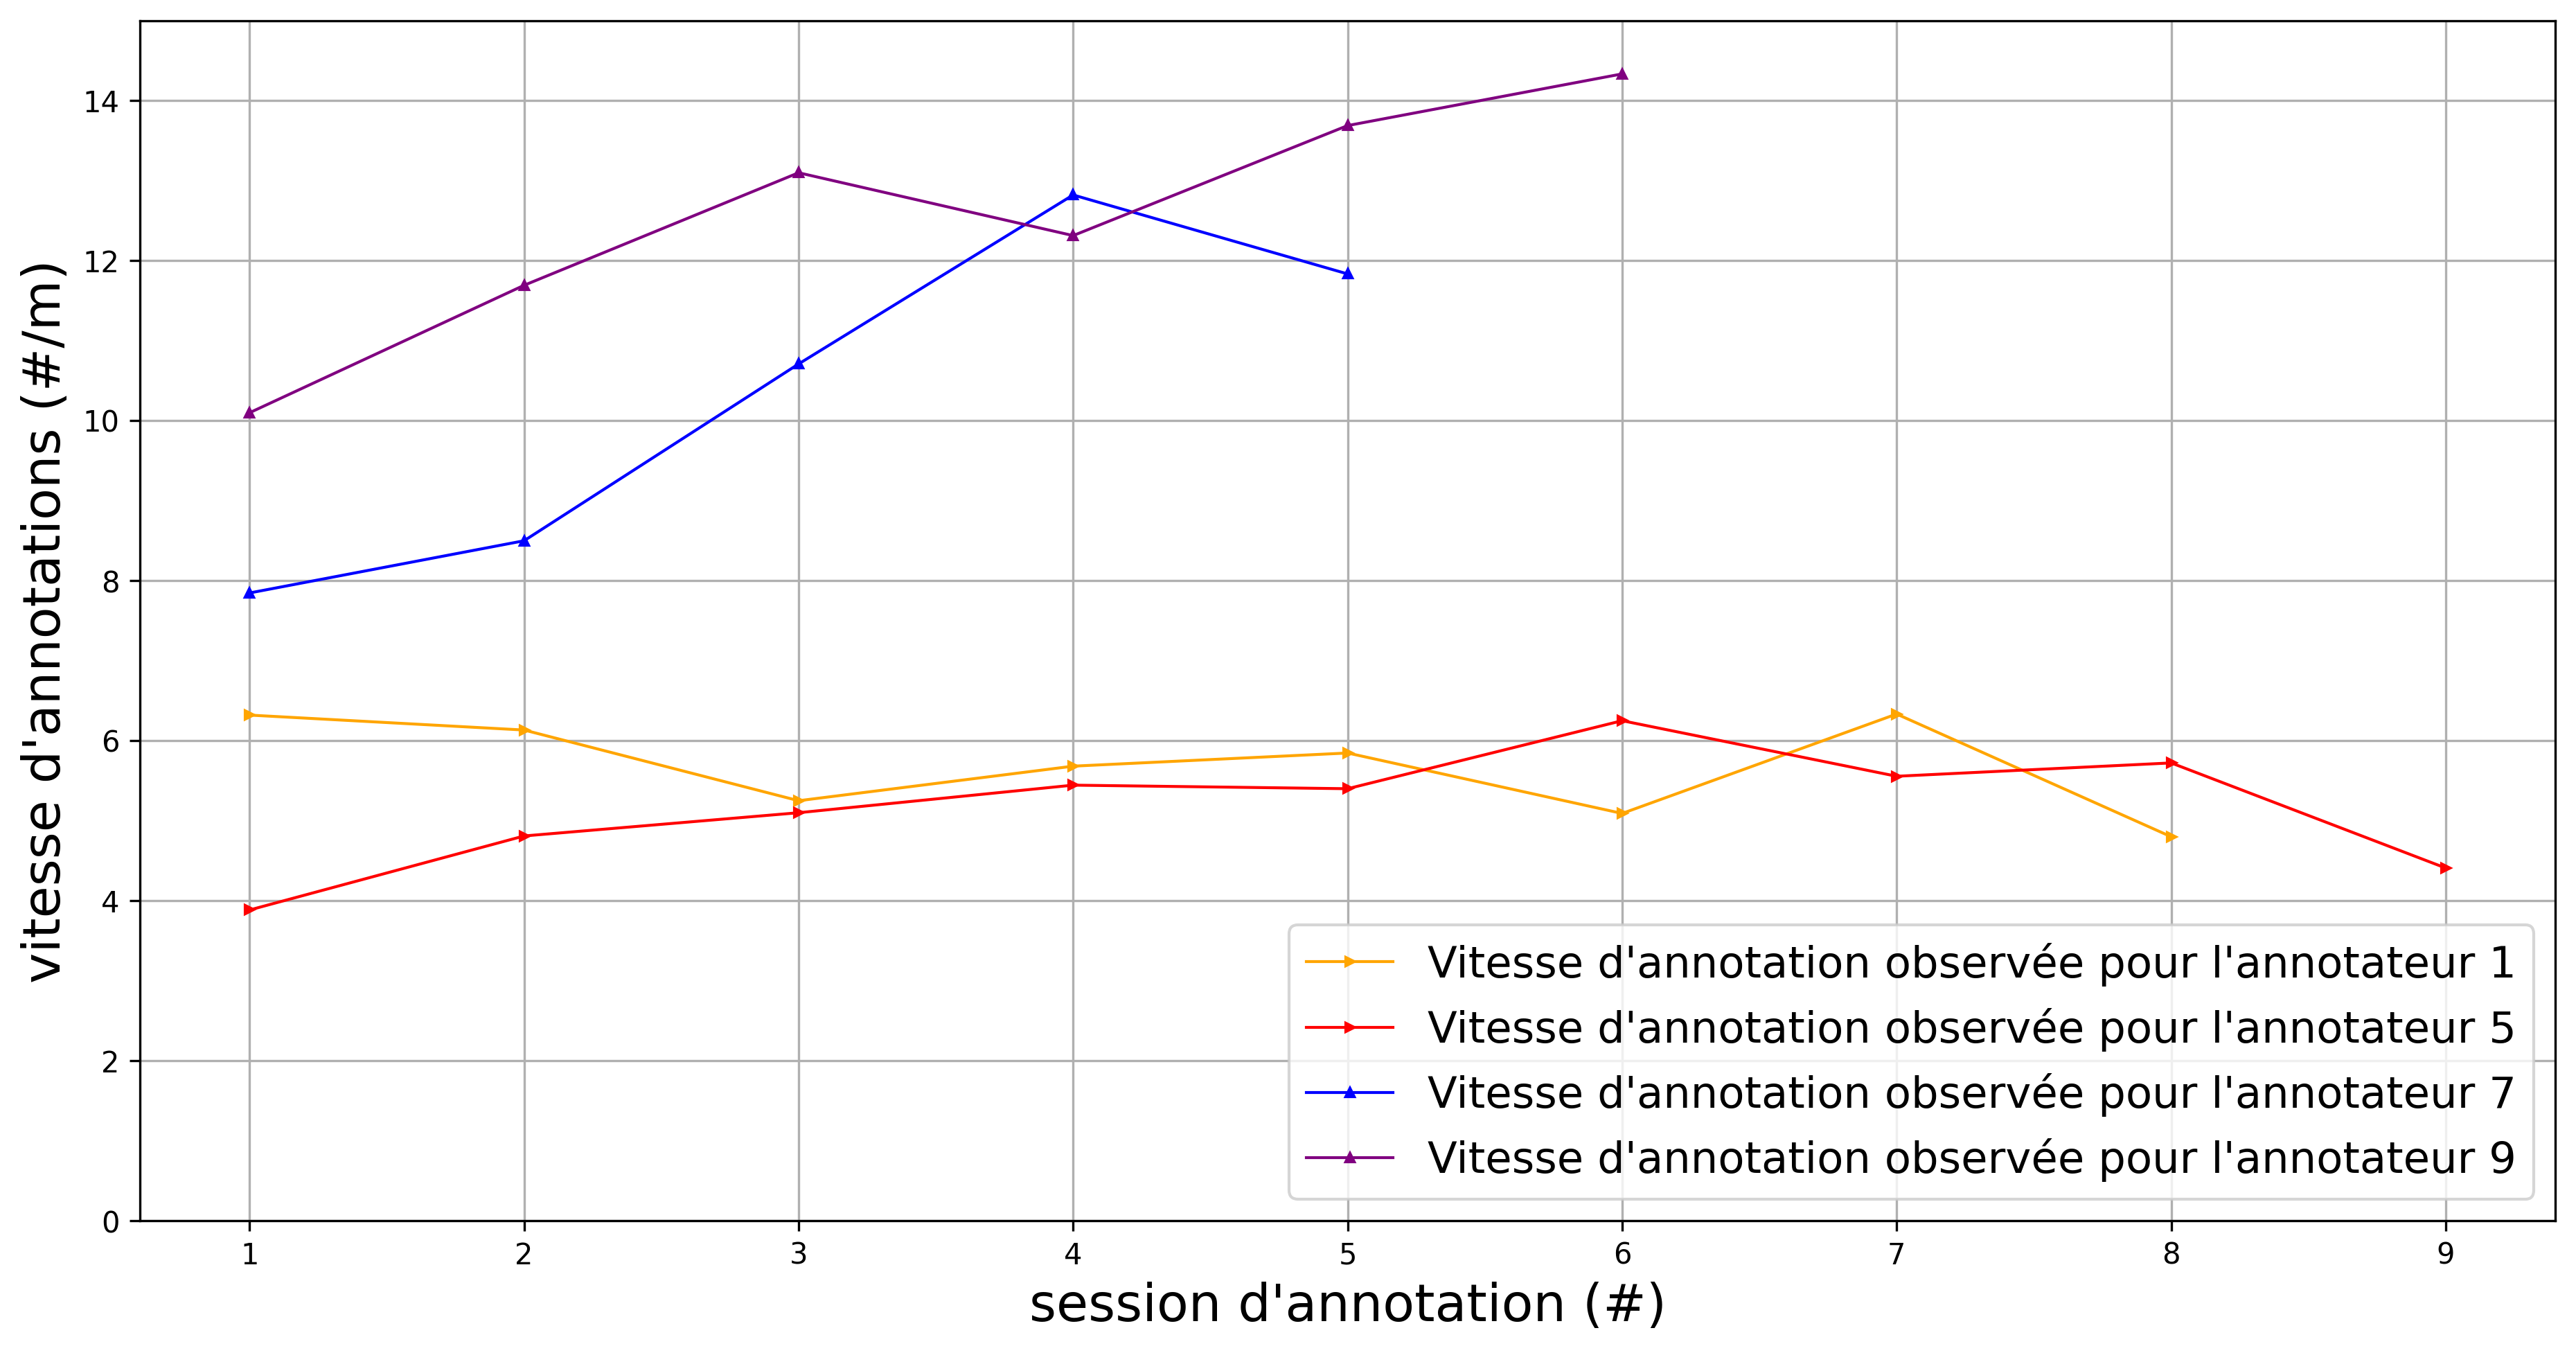
\includegraphics[width=0.95\textwidth]{figures/etude-temps-annotation-3-etude-de-cas}
				\caption{
					Étude de cas d'évolution de la vitesse d'annotation de contraintes (en contraintes par minutes) en fonction des différentes sessions d'annotations.
				}
				\label{figure:4.3.1-ETUDE-COUTS-TEMPS-ANNOTATION-EXEMPLE}
			\end{figure}

		%%% Discussion.
		\subsubsection{Discussion}

		
		% Généralités sur la modélisation du temps d'annotation sur une session.
		L'étude réalisée avec $14$ annotateurs sur des lots de $1~000$ contraintes a permis d'estimer à $7.8 \cdot \texttt{batch\_size}$ le temps nécessaire (en secondes) pour annoter un lot de contraintes (cf. \textsc{Figure~\ref{figure:4.3.1-ETUDE-COUTS-TEMPS-ANNOTATION-SIMULATION}}).
		
		% Compliqué de comparer ...
		\begin{leftBarAuthorOpinion}
			Avant poursuivre la discussion, il est nécessaire de préciser qu'il est difficile de comparer ces résultats.
			% Forte disparité des mesures.
			D'une part, il y a une forte disparité des mesures, et il est idyllique de penser qu'une étude sur $14$ annotateurs peut représenter la diversité du comportement humain sur une tâche aussi complexe que l'annotation de données textuelles.
			% Peu de repères concrets.
			D'autre part, il y a un manque de repères concrets dans la littérature scientifique, entre autres à cause des nombreux facteurs intervenant dans une tâche d'annotation (\textit{objectifs à réaliser, données à manipuler, nombre de choix proposés à l'opérateur, complexité sémantique des données, des compétences de l'opérateur, fréquence d'exécution de la tâche, ...}), mais aussi en raison du manque d'intérêt à l'analyse du temps nécessaire au profit de l'analyse de la cohérence et de la qualité intra- ou inter-annotateur (\cite{baledent:2022:complexite-annotation-manuelle}).
			% Diversité des données.
			De plus, les résultats peuvent différer en fonction des contraintes à caractériser : on peut supposer que des couples de données très similaires ou très différentes sont simples à annoter, mais que des données plus ambiguës peuvent nécessiter davantage de temps pour être intégrées et étiquetées.
			
			% Angle d'attaque.
			Pour pallier ce problème, nous proposons confronter nos estimations à des mesures réalisées sur des tâches n'ayant pas le même objectif mais dont la complexité est comparable.
			Cette approche, bien qu'un peu rudimentaire, nous permettra ainsi de discuter des ordres de grandeurs à manipuler.
		\end{leftBarAuthorOpinion}
		
		
		%%% A. Analyse de l'annotation d'une contraintes.
		\paragraph{Analyse de l'annotation d'une contraintes.}
		
			% Avantage 1: 8 secondes, c'est acceptable.
			En premier lieu, nous voulions confirmer que l'annotation de contraintes est une tâche intuitive dont la durée est est caractéristique d'un mécanisme de réaction et non d'une réflexion.
			Pour ce faire, nous avons estimé la durée théorique d'une annotation à $7$ secondes par contrainte, comprenant les temps de lecture, d'analyse de la similitude et d'action de l'opérateur, et nous avons mesuré la durée d'annotation réelle à $7.8$ secondes par contrainte.
			Bien que l'écart constaté ($0.8$ seconde) soit compris dans les bornes d'approximation, cette différence n'est pas suffisamment insignifiante pour nous permettre d'exclure avec certitude la présence d'un mécanisme cognitif supplémentaire.
				
			% Avantage 2: Dans tous les cas, 8 secondes, c'est mieux que 17 secondes ou 40 secondes.
			Pour nous permettre de discuter du temps d'annotation mesuré et de son approximation théorique, nous utilisons utiliser plusieurs points de référence extraits de (\cite{snow-etal:2008:cheap-fast-it}).
			Dans cette étude, les auteurs délèguent quelques tâches d'annotation à \texttt{Amazon Mechanical Turk}\footnote{
				\texttt{Amazon Mechanical Turk} est une plateforme de travail collaboratif en ligne (\textit{crowdsourcing}) : nous avions évoqué leur fonctionnement, leur avantages et leurs inconvénients en \textsc{Section~\ref{section:2.3.2.C-DEFIS-ANNOTATION-ASPECT-COMPLEXITE-COUTS}}, notamment le risque de l'abandon de la qualité des annotations au profit de la quantité.
			} :
			
			\begin{enumerate}
				% Task 1: (Word Sense Disambiguation)
				\item Tâche de "\textit{désambiguïsation du sens des mots}" (\cite{pradhan-etal:2007:semeval2007-task-17}) :
				Elle consiste à catégoriser le contexte de phrases comportant le mot "\textit{président}" suivant $3$ options préformatées (\textit{dirigeant d'une entreprise, dirigeant des États Unis, dirigeant d'un autre pays}).
				Il y a $177$ phrases à labelliser par $10$ annotateurs, et la tâche a été réalisée en un total de $8.59$ heures, soit une moyenne de $17.5$ secondes par annotation.
				Nous utilisons ce point de repère car la tâche s'apparente à une annotation d'une tâche de classification ($3$ catégories).
				% Task 2: (Word Similarity)
				\item Tâche de "\textit{caractérisation de similitude des mots}" (\cite{miller-charles:1991:contextual-correlates-semantic}) :
				Elle consiste à ordonner des couples de mots du plus similaire au moins similaire en fonction de leur proximité sémantique afin de mettre en avant les meilleurs couples de synonymes.
				Il y a $30$ paires de synonymes à ordonner par $10$ annotateur, et la tâche a été réalisée en un total de $0.17$ heures, soit une moyenne de $2.0$ secondes par annotation.
				Nous utilisons ce point de repère car la tâche s'apparente à l'annotation de contraintes (\textit{laquelle de ces deux paires est la plus adéquate ?}) qui ne fait pas appel à un mécanisme de réflexion (\textit{peu de vocabulaire, similarité intrinsèque triviale entre deux mots}).
				% Task 3: (Recognizing Textual Entailment)
				\item Tâche de "\textit{reconnaissance de l'implication textuelle}" (\cite{dagan-etal:2005:pascal-recognising-textual}) :
				Elle consiste à confirmer ou infirmer si une phrase est la conséquence d'une autre (\textit{l'annotation est donc binaire}).
				Il y a $800$ paires de phrases à valider par $10$ annotateur, et la tâche a été réalisée en un total de $89.3$ heures, soit une moyenne de $40.2$ secondes par annotation.
				Nous utilisons ce point de repère car la tâche s'apparente à l'annotation de contraintes (\textit{est-ce que l'implication est vraie ?}) faisant intervenir un mécanisme de réflexion (\textit{comprendre une implication logique}).
			\end{enumerate}
			%
			% Comparaison à Task 1: (Word Sense Disambiguation).
			En utilisant la tâche de "\textit{désambiguïsation du sens des mots}" (1.), nous avons déjà un point de comparaison entre notre annotation de contraintes et une annotation classique de classes.
			Nous constatons une nette différence entre les deux approches ($7.8$ secondes par contrainte vs $17.5$ secondes par donnée), cela met en avant qu'une annotation de contraintes est plus rapide qu'une annotation par label.
			
			% Comparaison à Task 2: (Word Similarity).
			Ensuite, en utilisant la tâche de "\textit{caractérisation de similitude des mots}" (2.), nous pouvons confirmer que notre approximation théorique (faisant intervenir un traitement cognitif de $1$ seconde) semble adaptée pour représenter un mécanisme de l'ordre de la réaction.
			En effet, le coût très faible de la caractérisation d'une similarité entre deux mots ($2.0$ secondes par paire de mots) s'avère être en adéquation avec cette approximation ($2.5$ secondes par paire de phrases de taille $1$).
			
			% Comparaison à Task 3: (Recognizing Textual Entailment).
			Enfin, en utilisant la tâche de "\textit{reconnaissance de l'implication textuelle}" (3.), nous comparons deux annotations binaires dont une fait nettement appel à un mécanisme de réflexion (déduction logique dans une implication).
			Nous constatons une très nette différence entre les deux approches ($7.8$ secondes par contrainte vs $40.2$ secondes par implication), ce qui nous permet d'exclure la présence de mécanisme cognitif trop complexe.
	
			% Conclusion sur l'analyse de l'annotation d'une contraintes.
			\begin{leftBarSummary}
				Mettant bout à bout ces comparaisons, et en gardant à l'esprit que ces références restent approximatives, nous pouvons conclure que (1) \textbf{l'annotation de contraintes est une tâche plus rapide qu'une annotation par label} et que (2) \textbf{cette annotation binaire ne semble pas faire pas intervenir de traitement cognitif complexe} (\textit{c'est une piste à explorer plus en détails pour expliquer le gain de temps observé}).
			\end{leftBarSummary}
		
		
		%%% B. Analyse d'une session d'annotation de contraintes.
		\paragraph{Analyse d'une session d'annotation de contraintes.}
		
			% Ouverture 1: Autres analyses sans conclusions.
			Nous avons analysé l'évolution de la vitesse d'annotation au cours des sessions d'annotation, en espérant observer une accélération des annotations au fur et à mesure que l'annotateur s'habitue avec la tâche, ainsi qu'un effet de fatigue pour des sessions d'annotations trop longues.
			Cependant, aucune de nos analyses n'a montré de résultats significatifs (on peut constater la forte dispersion des résultats grâce à la \textsc{Figure~\ref{figure:4.3.1-ETUDE-COUTS-TEMPS-ANNOTATION-EXEMPLE}}).
			Nous ne pouvons donc pas conclure sur de telles tendances.
			
			\begin{leftBarAuthorOpinion}
				Nos intuitions initiales concernaient deux points :
				\begin{itemize}
					% Temps d'adaptation.
					\item la diminution du \textbf{temps d'adaptation} au cours de sessions d'annotations : au fur et à mesure qu'il annote, l'opérateur pourrait entrer plus facilement dans sa tâche, lui permettant d'atteindre plus rapidement sa vitesse de croisière et ainsi gagner en efficacité sur plusieurs sessions.
					D'après \cite{anderson:2013:architecture-cognition}, ce temps d'adaptation pourrait se définir en trois étapes : une phase déclarative (\textit{besoin d'instructions détaillées, exécution lente et avec erreurs}), une phase associative (\textit{quelques rappels clés suffisent pour retrouver les instructions, donc gain de vitesse}) et une phase autonome (\textit{les consignes sont acquises, donc exécution rapide et sans erreur}) ;
					% Effet de fatigue.
					\item l'intervention d'un \textbf{effet de fatigue} : si une session d'annotation dure trop longtemps, l'opérateur pourrait perdre en efficacité par manque de concentration et augmenter ses chances de faire des erreurs.
					D'après \cite{jones-etal:2015:demographic-occupational-predictors}, la fatigue est considérée comme un inconfort qui s'installe après une tâche excessive, et \cite{elkosantini-gien:2009:integration-human-behavioural} décrit cet état de fatigue par des capacités de travail réduites.
				\end{itemize}
				%
				Ces différentes intuitions ont aussi été remontées par les annotateurs de notre expériences, mais aucun effet significatif n'a pu être observé.
			\end{leftBarAuthorOpinion}
		
			% Ouverture 2: Remarque sur le nombre maximal moyen de contraintes à annoter.
			Par extension, nous ne pouvons pas non plus conclure sur la taille optimale d'échantillon de contraintes à sélectionner pour une session d'annotation.
			Dans nos précédentes études, nous avions arbitrairement fixé la taille de lot à $50$ pour bénéficier d'itérations brèves, permettant à l'algorithme de \textit{clustering} de l'améliorer régulièrement avec les dernières contraintes.
			Mais des petits lots d'annotation démultiplient le nombre d'itérations à réaliser, et donc le nombre d'algorithmes à exécuter.
			Il serait donc judicieux d'adapter le nombre d'annotations à réaliser pour d'améliorer l'expérience utilisateur en situation réelle de l'opérateur.
			Malheureusement, aucun repère significatif ne peut être déduit de nos résultats pour prédire la fin d'un temps d'adaptation ou le début d'un effet de fatigue.
			
			% Idées : nombre de contraintes moyen par session.
			Afin de proposer tout de même un ordre de grandeur de taille de lot, nous pouvons nous intéresser au nombre moyen de contraintes annotées lors des sessions réalisées par les opérateurs de notre expérience.
			Bien que ces informations n'ont pas été collectées initialement à cette fin, on peut supposer que les opérateurs ont interrompu leur session pour se reposer (\textit{par fatigue, ennui, agacement, ...}) ou répondre à une autre sollicitation (\textit{intervention d'un collègue, mail important, pause café, ...})
			Après un entretien avec les opérateurs de notre expérience, il semble y avoir deux possibilités : soit l'opérateur ne se fixait pas d'objectif et s'arrêtait par fatigue ; soit il se fixait un objectif (\textit{de nombre ou de durée}), mais adaptait son prochain objectif en fonction de la fatigue ressentie en fin de session.
			Dans les deux cas, nous pouvons faire l'hypothèse que le nombre moyen d'annotation par session tend à représenter une borne supérieure de la taille maximale d'un lot à considérer pour ne pas entamer l'effet de fatigue.
			Sur l'expérience réalisée, cette moyenne est de $170.70$ contraintes annotées par session (écart-type: $106.37$, erreur standard: $13.19$).
			En prenant en compte une marge d'erreur pour minimiser ce résultat, nous retenons $150$ contraintes comme seuil à ne pas dépasser.
			
			% Conclusion sur l'analyse d'une session d'annotation de contraintes.
			\begin{leftBarSummary}
				Pour une session d'annotation, \textbf{nous conseillons une taille d'échantillon entre $50$ et $150$ contraintes}.
				Attention aux échantillons trop petits qui multiplient le nombre d'itérations à réaliser ;
				Attention aussi aux échantillons trop gros qui peuvent introduire un effet de fatigue chez l'opérateur et casser la dynamique d'interactions avec la machine.
				La discussion finale de ce chapitre affinera cette fourchette grâce à une vue d'ensemble sur les coûts de la méthode.
			\end{leftBarSummary}
			

		%%% C. Analyse des fonctionnalités de l'application d'annotation
		\paragraph{Analyse des fonctionnalités de l'application d'annotation.}
		
			% Ouverture 3: Autres remontées applicatives.
			Pour finir cette discussion, nous nous intéressons à l'utilisation du logiciel par nos opérateurs au cours de cette étude.
			En effet, il est logique de penser que la conception de l'application et les fonctionnalités qu'elle dispose peut grandement impacter l'expérience utilisateur de notre méthodologie de \textit{clustering} itératif.
			Un entretien avec les opérateurs a permis de remonter plusieurs pistes d'amélioration sur son ergonomie.
			
			% Idées 1: Données non prétraitées.
			Un premier point concerne l'affichage des textes d'une contraintes.
			Comme montré en \textsc{Figure~\ref{figure:4.3.1-ETUDE-COUTS-TEMPS-ANNOTATION-APPLICATION-ANNOTATION}}, nous avions choisi d'affichée des données normalisées à l'écran pour masquer le bruit provoqué par les accents, les majuscules, la ponctuation.
			Bien que cette fonctionnalité peut servir pour des textes bruts (issues de conversation clients ou de forum par exemple), cela a plutôt nuit à la compréhension des données par les opérateurs.
			Nous avons donc envisager de laisser la données brutes à disposition, dans une infobulle ou grâce à une option permettant d'interchanger le format des données.
			
			% Idée 2: Ordonner les données.
			Une seconde proposition concerne l'ordre des contraintes à annoter.
			Nous pouvons facilement admettre que la compréhension rapide d'un grand nombre de texte est un tâche pénible.
			Pour soulager les opérateurs et limiter le nombre de transitions, nous avons trier les contraintes par ordre alphabétique.
			Ainsi, toutes les contraintes associées à une même donnée peuvent être traitées à la suite.
			Cette solution permet de limiter le nombre de changement de contexte et peut faciliter la caractérisation d'une similitude en analysant à la chaîne plusieurs données du même type.
			À cet effet, une option e tri à été ajouté sur la liste de contraintes à traiter (cf. \textsc{Figure~\ref{figure:4.3.1-ETUDE-COUTS-TEMPS-ANNOTATION-APPLICATION-LISTE-CONTRAINTES}}).
			
			% Idée 3: Annotation multi-contraintes.
			Enfin, une dernière idée concerne l'affichage des données à annoter.
			Nous avions jusqu'à présent considérer l'annotation entre deux données (cf. \textsc{Figure~\ref{figure:4.3.1-ETUDE-COUTS-TEMPS-ANNOTATION-APPLICATION-ANNOTATION}}), mais il peut être judicieux d'afficher plusieurs données à caractériser simultanément.
			Une telle fonctionnalité permettrait ainsi de regrouper rapidement un grand nombre de données similaires ou de distinguer avec moins d'ambiguïté certaines données en s'appuyant sur leur voisinage.
			
			\begin{leftBarInformation}
				Ces différentes évolutions sont en cours d'analyse ou ont déjà été intégrées dans l'application que nous proposons (\cite{schild-etal:2022:cognitivefactory-interactiveclusteringgui}).
			\end{leftBarInformation}
	

	%%%
	%%% Subsection 4.3.2: Étude du temps de calcul nécessaire aux algorithmes implémentés en chronométrant des exécutions dans différentes situations
	%%%
	\subsection{Étude du temps de calcul nécessaire aux algorithmes implémentés en chronométrant des exécutions dans différentes situations}
	\label{section:4.3.2-ETUDE-COUTS-TEMPS-CALCUL}
		
		% Transition.
		Maintenant que nous avons pu modéliser le temps nécessaire à un expert pour annoter un lot de contraintes, nous nous intéressons au temps nécessaire à la machine pour interpréter ces annotations et proposer une nouvelle segmentation des données.
		
		% Complexité de la tâche.
		Comme les différents algorithmes employés manipulent des contraintes sur les données, l'estimation théorique du temps d'exécution par l'analyse de la complexité ne semble pas fiable : en effet, quelques contraintes bien placées peuvent suffire à simplifier le fonctionnement d'un algorithme de \textit{clustering} alors qu'une grande quantité de contraintes mal placées vont au contraire le pénaliser.
		% Objectif de l'expérience.
		Nous préférons donc une approche empirique en chronométrant plusieurs exécutions isolées des algorithmes intervenant dans notre implémentation du \textit{clustering} interactif et en évaluant l'importance de leurs différents arguments d'entrée (la taille du jeu de données, le nombre de clusters et le nombre de contraintes annotées, ...).
		Nous profitons aussi de ces modélisations du temps de calcul pour confirmer le choix de paramétrage réalisé lors de l'étude d'efficience en \textsc{Section~\ref{section:4.2-HYPOTHESE-EFFICIENCE}}, et ainsi faire un compromis entre l'algorithme le plus efficient et l'algorithme le plus rapide.
	
		%%% Protocole expérimental.
		\subsubsection{Protocole expérimental}
			
			% Pseudo-code.
			Pour résumer le protocole expérimental que nous décrivons ci-dessous, vous pouvez vous référer aux pseudo-code décrit dans \textsc{Algorithme~\ref{algorithm:4.3.2-ETUDE-COUTS-TEMPS-CALCUL-PROTOCOLE}}.
			
			\begin{algorithm}
				\KwData{jeux de données annotées (vérités terrains) de tailles différentes}
				\KwIn{combinaisons d'algorithmes et de paramètres à tester}
				%
				\ForEach{combinaison d'algorithmes et de paramètres à tester}{
					\textbf{initialisation (données)}: récupérer ou générer le jeu de données \;
					\textbf{initialisation (contraintes)}: créer une liste vide de contraintes \;
					\If{estimation de la tâche de \textbf{prétraitement}}{
						\textbf{chronomètre}: \textbf{START} \;
						\textbf{prétraitement (à étudier)}: supprimer le bruit dans les données \;
						\textbf{chronomètre}: \textbf{STOP} \;
					}
					\ElseIf {estimation de la tâche de \textbf{vectorisation}}{
						\textbf{prétraitement}: supprimer le bruit dans les données avec \texttt{prep.simple} \;
						\textbf{chronomètre}: \textbf{START} \;
						\textbf{vectorisation (à étudier)}: transformer les données en vecteurs \;
						\textbf{chronomètre}: \textbf{STOP} \;
					}
					\ElseIf {estimation de la tâche de \textbf{clustering}}{
						\textbf{prétraitement}: supprimer le bruit dans les données avec \texttt{prep.simple} \;
						\textbf{vectorisation}: transformer les données en vecteurs avec \texttt{vect.tfidf} \;
						\textbf{échantillonnage initial}: sélectionner des contraintes avec \texttt{samp.rand.full} \;
						\textbf{simulation d'annotation}: déterminer les contraintes avec la vérité terrain \;
						\textbf{intégration}: ajouter les nouvelles contraintes au gestionnaire de contraintes \;
						\textbf{chronomètre}: \textbf{START} \;
						\textbf{clustering (à étudier)}: regrouper les données par similarité \;
						\textbf{chronomètre}: \textbf{STOP} \;
					}
					\ElseIf {estimation de la tâche d'\textbf{échantillonnage}}{
						\textbf{prétraitement}: supprimer le bruit dans les données avec \texttt{prep.simple} \;
						\textbf{vectorisation}: transformer les données en vecteurs avec \texttt{vect.tfidf} \;
						\textbf{échantillonnage initial}: sélectionner des contraintes avec \texttt{samp.rand.full} \;
						\textbf{simulation d'annotation}: déterminer les contraintes avec la vérité terrain \;
						\textbf{intégration}: ajouter les nouvelles contraintes au gestionnaire de contraintes \;
						\textbf{clustering initial}: regrouper les données avec \texttt{clust.kmeans.cop} \;
						\textbf{chronomètre}: \textbf{START} \;
						\textbf{échantillonnage (à étudier)}: sélectionner de nouvelles contraintes à annoter \;
						\textbf{chronomètre}: \textbf{STOP} \;
					}
				}
				\ForEach{algorithme à modéliser}{
					\textbf{cadrage}: définir les facteurs et les interactions intervenant dans la modélisation \;
					\textbf{simplification}: restreindre la modélisation aux facteurs les plus corrélés \;
					\textbf{analyse}: modéliser le temps d'exécution avec les facteurs retenus \;
				}
				%
				\KwResult{modélisation du temps d'exécution des différents algorithmes}
				%
				\caption{\textit{
					Description en pseudo-code du protocole expérimental de l'étude du temps d'exécution des algorithmes du \textit{clustering} interactif.
				}}
				\label{algorithm:4.3.2-ETUDE-COUTS-TEMPS-CALCUL-PROTOCOLE}
			\end{algorithm}
			
			% Description de la vérité terrain.
			Nous utilisons le jeu de données \texttt{Bank Cards (v2.0.0)} comme référence pour cette expérience : ce dernier traite des demandes les plus fréquentes des clients en ce qui concerne la gestion de leur carte bancaire.
			Il est composé de $1~000$ questions rédigées en français et réparties en $10$ classes (\texttt{perte ou vol de carte}, \texttt{carte avalée}, \texttt{commande de carte}, ...).
			Pour plus de détails, consultez l'annexe~\ref{annex:A.1-DATASET-BANK-CARDS}.
			Cependant, un seul jeu de données ne nous permet pas d'analyser l'impact du nombre de données sur le temps d'exécution des algorithmes.
			Pour utiliser facilement plusieurs jeux de données de tailles différentes tout en maîtrisant leur contenu, nous avons donc dupliqué aléatoirement des données issues du jeu de référence en y insérant des fautes de frappes.
			
			% Remarques.
			\begin{leftBarWarning}
				Dans le cadre de cette étude, nous faisons l'hypothèse que cette création artificielle de données n'a pas d'impact majeur sur le temps d'exécution des différents algorithmes.
			\end{leftBarWarning}
			
			% Description des tâches, des algorithmes et des contextes.
			À l'aide de ces données, nous lançons plusieurs exécutions de chaque algorithme de notre implémentation du \textit{clustering} interactif (cf. \textsc{Section~\ref{section:3.3-DESCRIPTION-IMPLEMENTATION}}) avec différentes variations de contexte d'utilisation.
			Cela comprend les tâches, algorithmes et contextes d'utilisation suivants :
			\begin{enumerate}
				% Prétraitement.
				\item le \textbf{prétraitement} des données...
					\begin{itemize}
						\item avec les algorithmes suivants : \textbf{simple} (noté \texttt{prep.simple}), \textbf{avec lemmatisation} (noté \texttt{prep.lemma}) et \textbf{avec filtres} (noté \texttt{prep.filter}) ;
						\item avec les contextes d'utilisation suivants : \textbf{nombre de données} (variant de $1~000$ à $5~000$ par pas de $1~000$, noté $\texttt{dataset\_size}$) ;
					\end{itemize}
				% Vectorisation.
				\item la \textbf{vectorisation} des données...
					\begin{itemize}
						\item avec les algorithmes suivants : \textbf{TF-IDF} (noté \texttt{vect.tfidf}) et \textbf{SpaCy} (noté \texttt{vect.frcorenewsmd}) ;
						\item avec les contextes d'utilisation suivants : \textbf{nombre de données} (variant de $1~000$ à $5~000$ par pas de $1~000$, noté $\texttt{dataset\_size}$) ;
						\item précédé par un prétraitement \textbf{simple} ;
					\end{itemize}
				% Clustering.
				\item le \textbf{\textit{clustering} sous contraintes} des données...
					\begin{itemize}
						\item avec les algorithmes suivants : \textbf{KMeans} (modèle \textit{COP} noté \texttt{clust.kmeans.cop}), \textbf{Hiérarchique} (lien \textit{single} noté \texttt{clust.hier.sing} ; lien \textit{complete} noté \texttt{clust.hier.comp} ; lien \textit{average} noté \texttt{clust.hier.avg} ; lien \textit{ward} noté \texttt{clust.hier.ward}) et \textbf{Spectral} (modèle \textit{SPEC} noté \texttt{clust.spec}) ;
						\item avec les contextes d'utilisation suivants : \textbf{nombre de données} (variant de $1~000$ à $5~000$ par pas de $1~000$, noté $\texttt{dataset\_size}$), le \textbf{nombre de contraintes annotés} (variant de $0$ à $5~000$ par pas de $500$, noté $\texttt{previous\_nb\_constraints}$) et le \textbf{nombre de \textit{clusters} à trouver} (variant de $5$ à $50$ par pas de $5$, noté $\texttt{algorithm\_nb\_clusters}$) ;
						\item précédé par un prétraitement \textbf{simple} et une vectorisation \textbf{TF-IDF} et un échantillonnage initial \textbf{purement aléatoire} ;
					\end{itemize}
				% Sampling.
				\item l'\textbf{échantillonnage} des contraintes à annoter...
					\begin{itemize}
						\item avec les algorithmes suivants : \textbf{purement aléatoire} (noté \texttt{samp.random.full}), \textbf{pseudo-aléatoire} (noté \texttt{samp.random.same}), \textbf{même cluster et étant les plus éloignées} (noté \texttt{samp.farhtest.same}) et \textbf{clusters différents et étant les plus proches} (noté \texttt{samp.closest.diff}) ;
						\item avec les contextes d'utilisation suivants : \textbf{nombre de données} (variant de $1~000$ à $5~000$ par pas de $1~000$, noté $\texttt{dataset\_size}$), le \textbf{nombre de contraintes annotés} (variant de $0$ à $5~000$ par pas de $500$, noté $\texttt{previous\_nb\_constraints}$), le \textbf{nombre de \textit{clusters} existant} (variant de $10$ à $50$ par pas de $10$, noté $\texttt{previous\_nb\_clusters}$) et le \textbf{nombre de contraintes à sélectionner} (variant de $50$ à $250$ par pas de $50$, noté $\texttt{algorithm\_nb\_constraints}$) ;
						\item précédé par un prétraitement \textbf{simple}, une vectorisation \textbf{TF-IDF}, un \textit{clustering} initial \textbf{KMeans} (modèle \textit{COP}) et un échantillonnage initial \textbf{purement aléatoire} ;
					\end{itemize}
			\end{enumerate}
			
			Il y a donc $8~825$ combinaisons d'algorithmes (\texttt{15} pour le prétraitement, $10$ pour la vectorisation, $3~330$ pour le \textit{clustering}, $5~550$ pour l'échantillonnage), et chaque combinaison est répétée $5$ fois pour contrer les aléas statistiques des exécutions.
			De plus, chaque jeu de données est généré $5$ fois pour contrer les aléas statistiques de création, donc il y a $220~625$ exécutions d'algorithmes ($375$ pour le prétraitement, $250$ pour la vectorisation, $82~500$ pour le \textit{clustering}, $137~500$ pour l'échantillonnage).
			
			% Description de la modélisation.
			Sur la base de ces mesures, nous cherchons à modéliser le temps d'exécution de chaque algorithme en fonction de son contexte d'utilisation (dépendant de ses arguments d'entrée), et les interactions doubles entre paramètres sont envisagées.
			Afin de réduire la complexité des modélisations, nous ordonnons les interactions de facteurs possibles en fonction de leur corrélation avec le temps mesuré (la corrélation \texttt{r} de \textit{Pearson} (\cite{kirch:2008:pearson-correlation-coefficient}) est utilisée) et nous nous limitons aux variables responsables d'un maximum de la variance des mesures (la méthode d'\textit{Elbow} (\cite{thorndike:1953:who-belongs-family}) est utilisée pour choisir les facteurs pertinents).
			Sur cette base, nous entraînons un modèle linéaire généralisé (\textit{GLM}, cf. \cite{nelder-wedderburn:1972:generalized-linear-models}) pour représenter le temps d'exécution moyen de l'algorithme : ce modèle sera caractérisé par le coefficient de détermination généralisé \texttt{R²} de \textit{Cox et Snel} (\cite{diamond-etal:1990:analysis-binary-data}), la log-vraisemblance \texttt{llf} (\cite{edwards:1992:likelihood}) et la log-vraisemblance \texttt{llf\_null} du modèle \textit{null}.
			Pour finir, nous discutons des valeurs des coefficients obtenus sur l'impact du temps d'exécution.
			
			% Référence scripts.
			\begin{leftBarInformation}
				Les scripts de l'expérience, réalisés avec des \textit{notebooks} Python (\cite{van-rossum-drake:2009:python-reference-manual}), sont disponibles dans un dossier dédié de~\cite{schild:2021:cognitivefactory-interactiveclusteringcomparativestudy}.
				Nous utilisons entre autres les librairies \texttt{datetime} et \texttt{statsmodels} (\cite{seabold-perktold:2010:statsmodels-econometric-statistical}).
			\end{leftBarInformation}

		%%% Résultats.
		\subsubsection{Résultats obtenus}
				
			%%% Prétraitements
			
			% Première analyse.
			En ce qui concerne la tâche de \textbf{prétraitement}, une première analyse montre que les modélisations des trois implémentations sont similaires (\texttt{p-valeur}: $> 0.980$). Nous faisons donc une seule modélisation.
			
			% Modélisation du temps de calcul (prep.simple + prep.lemma + prep.filter).
			Pour les algorithmes de prétraitements (\texttt{prep.simple}, \texttt{prep.lemma} et \texttt{prep.filter}), l'analyse de la corrélation des facteurs avec les mesures de temps d'exécution indique qu'une modélisation minimale et suffisante peut être réalisée à partir du facteur $\texttt{dataset\_size}$ (\texttt{r}: $0.997$).
			Le modèle linéaire généralisé retenu (\texttt{R²}: $> 0.999$, \texttt{llf}: $-432.43$, \texttt{llf\_null}: $-1~353.98$) nous permet de déduire l'équation suivante :
			%
			\begin{equation}
				\texttt{computation\_time}(\texttt{prep})~[s]~
				\propto~6.55 \cdot 10^{-3} \cdot \texttt{dataset\_size}
			\end{equation}
			
			% Affichage du temps de calcul.
			La \textsc{Figure~\ref{figure:4.3.2-ETUDE-COUTS-TEMPS-CALCUL-MODELISATION-PREPROCESSING}} représente cette modélisation du temps de calcul des algorithmes de prétraitements en comparaison avec les mesures réalisées lors de l'expérience.
			\newline
			%
			\begin{figure}[!htb]
				\centering
				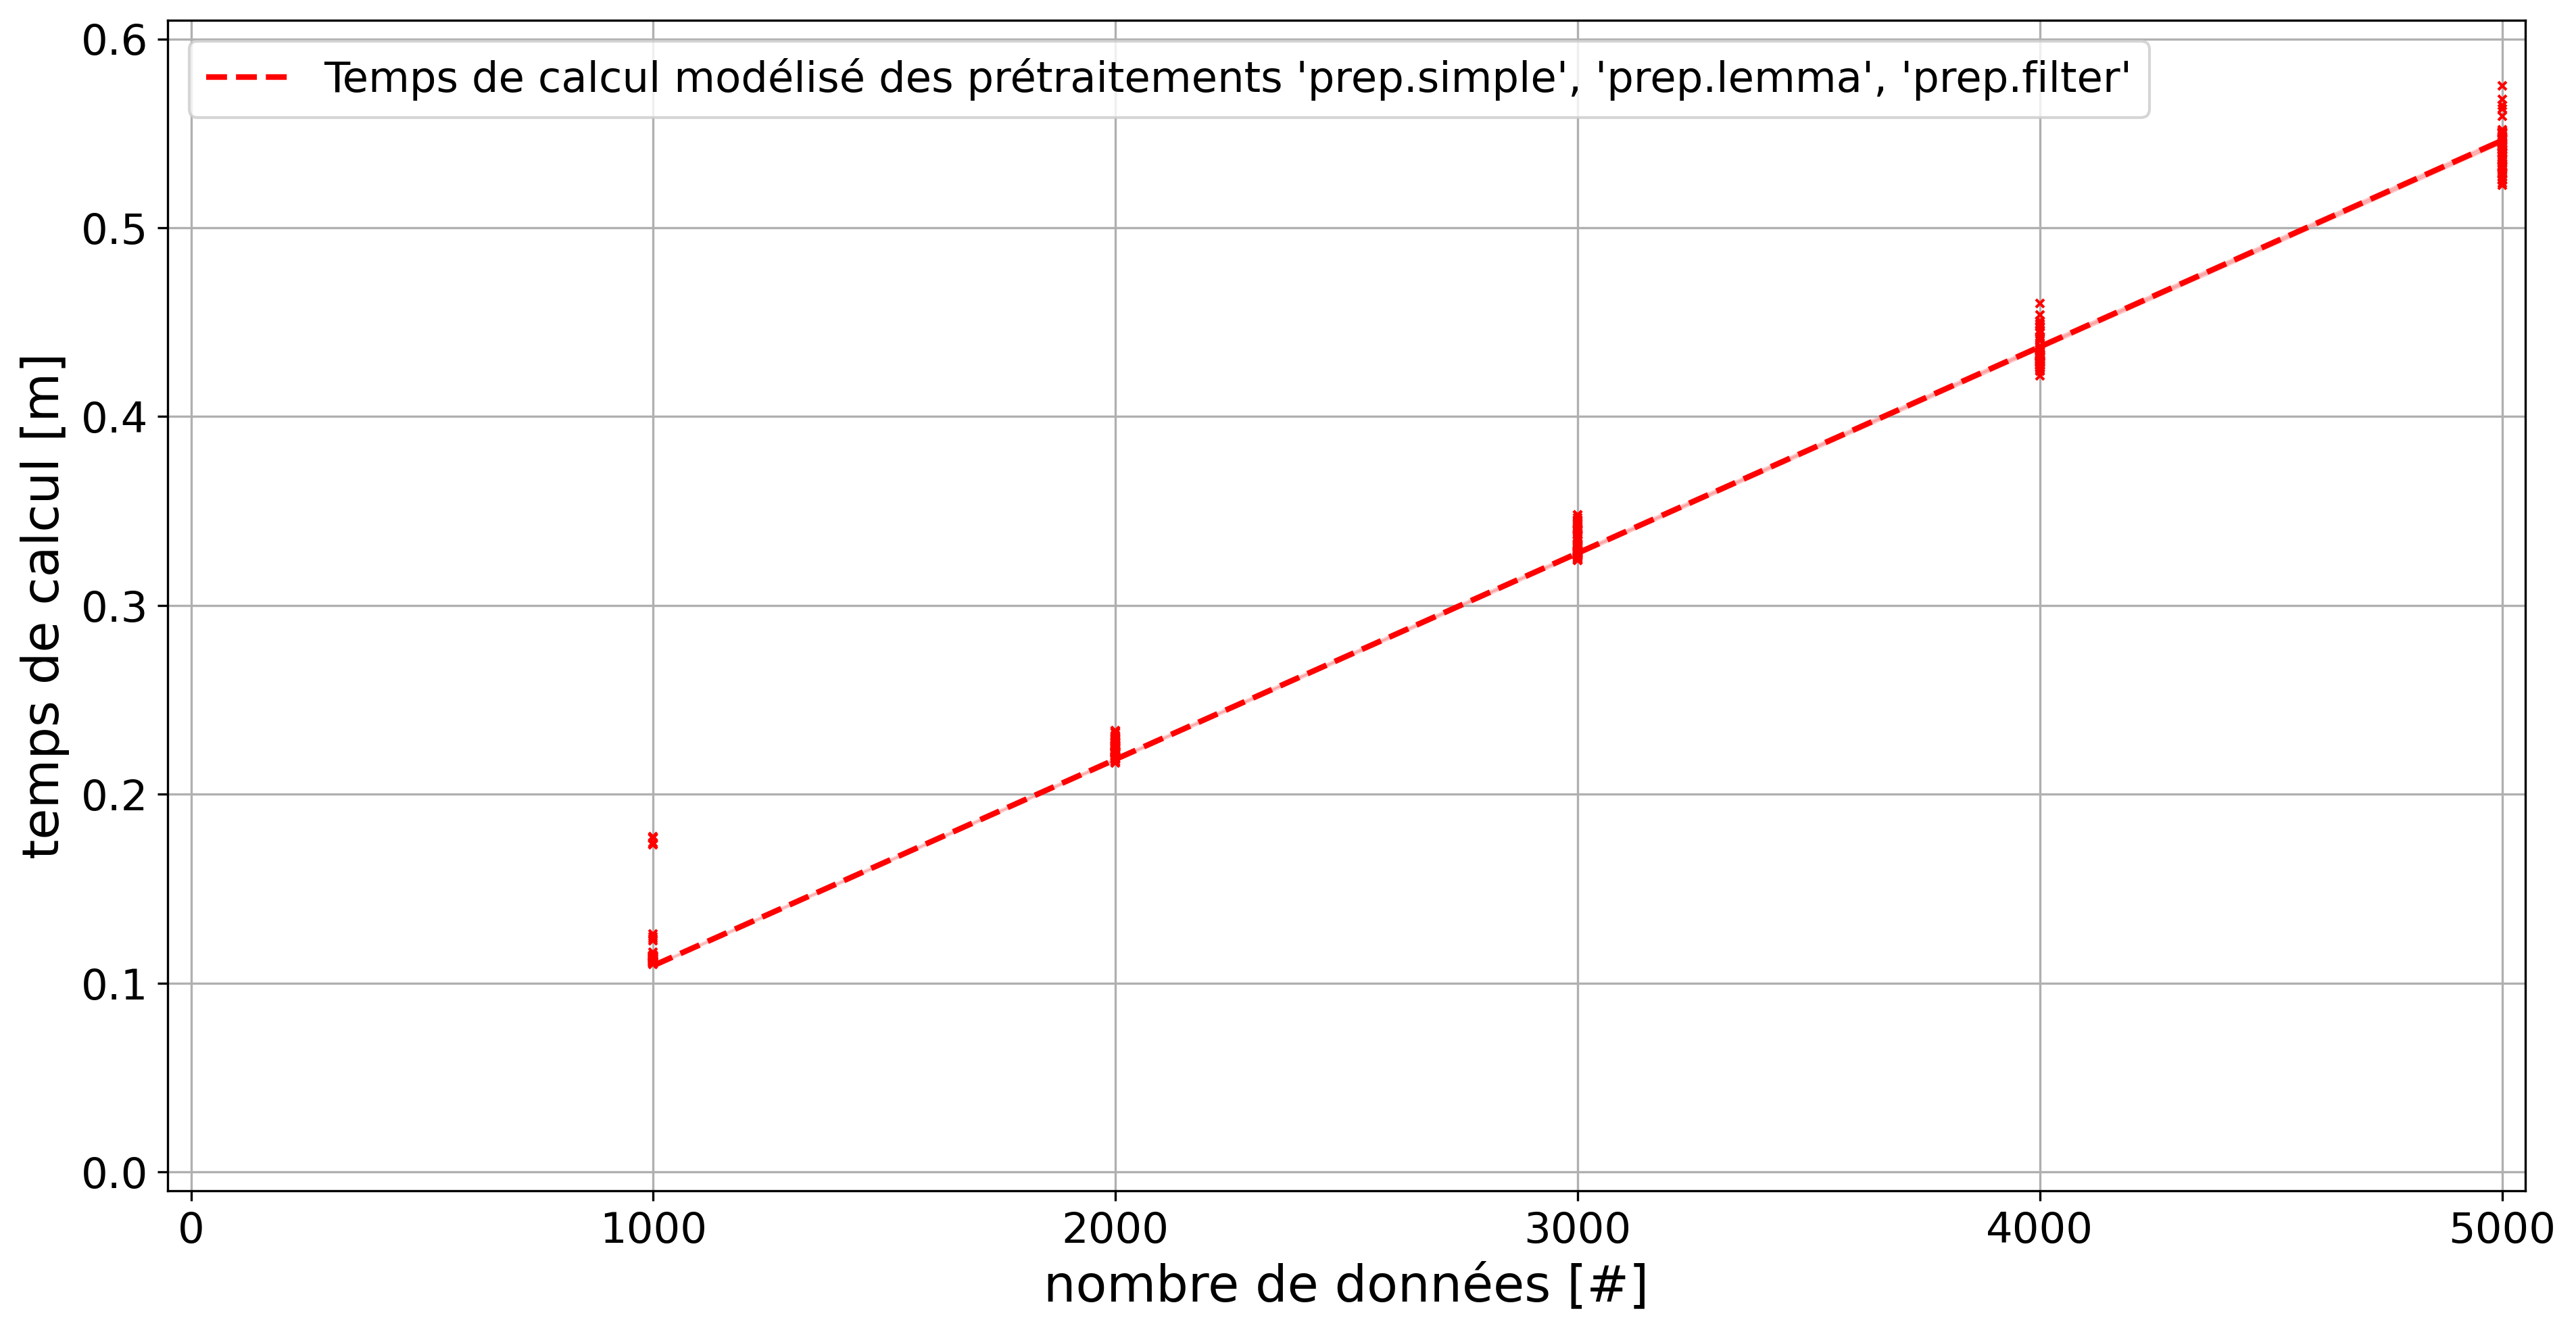
\includegraphics[width=0.95\textwidth]{figures/etude-temps-calcul-modelisation-1prep}
				\caption{
					Estimation du temps nécessaire (en minutes) pour effectuer une tâche de \textbf{prétraitement} en fonction du nombre de données à traiter. Les paramétrages \texttt{prep.simple}, \texttt{prep.lemma} et \texttt{prep.filter} ayant des temps de calculs similaires, leurs modélisations n'ont pas été séparées.
				}
				\label{figure:4.3.2-ETUDE-COUTS-TEMPS-CALCUL-MODELISATION-PREPROCESSING}
			\end{figure}
			
			%%% Vectorization
			
			% Première analyse.
			En ce qui concerne la tâche de \textbf{vectorisation}, une première analyse montre que les modélisations des deux implémentations sont différentiables (\texttt{p-valeur}: $< 10^{-3}$). Nous faisons donc une modélisation par algorithme.
		
			% Modélisation du temps de calcul (vect.tfidf).
			Pour les algorithmes de vectorisation \texttt{vect.tfidf}, l'analyse de la corrélation des facteurs avec les mesures de temps d'exécution indique qu'une modélisation minimale et suffisante peut être réalisée à partir du facteur $\texttt{dataset\_size}$ (\texttt{r}: $0.977$).
			Le modèle linéaire généralisé retenu (\texttt{R²}: $> 0.999$, \texttt{llf}: $259.89$, \texttt{llf\_null}: $70.04$) nous permet de déduire l'équation suivante :
			%
			\begin{equation}
				\texttt{computation\_time}(\texttt{vect.tfidf})~[s]~
				\propto~9.16 \cdot 10^{-5} \cdot \texttt{dataset\_size}
			\end{equation}
			
			% Modélisation du temps de calcul (vect.frcorenewsmd).
			Pour les algorithmes de vectorisation \texttt{vect.frcorenewsmd}, l'analyse de la corrélation des facteurs avec les mesures de temps d'exécution indique qu'une modélisation minimale et suffisante peut être réalisée à partir du facteur $\texttt{dataset\_size}$ (\texttt{r}: $0.983$).
			Le modèle linéaire généralisé retenu (\texttt{R²}: $> 0.999$, \texttt{llf}: $-214.44$, \texttt{llf\_null}: $-399.39$) nous permet de déduire l'équation suivante :
			%
			\begin{equation}
				\texttt{computation\_time}(\texttt{vect.frcorenewsmd})~[s]~
				\propto~4.62 \cdot 10^{-3} \cdot \texttt{dataset\_size}
			\end{equation}
			
			% Affichage du temps de calcul.
			La \textsc{Figure~\ref{figure:4.3.2-ETUDE-COUTS-TEMPS-CALCUL-MODELISATION-VECTORIZATION}} représente ces modélisations de temps de calcul des algorithmes de vectorisation en comparaison avec les mesures réalisées lors de l'expérience.
			\newline
			%
			\begin{figure}[!htb]
				\centering
				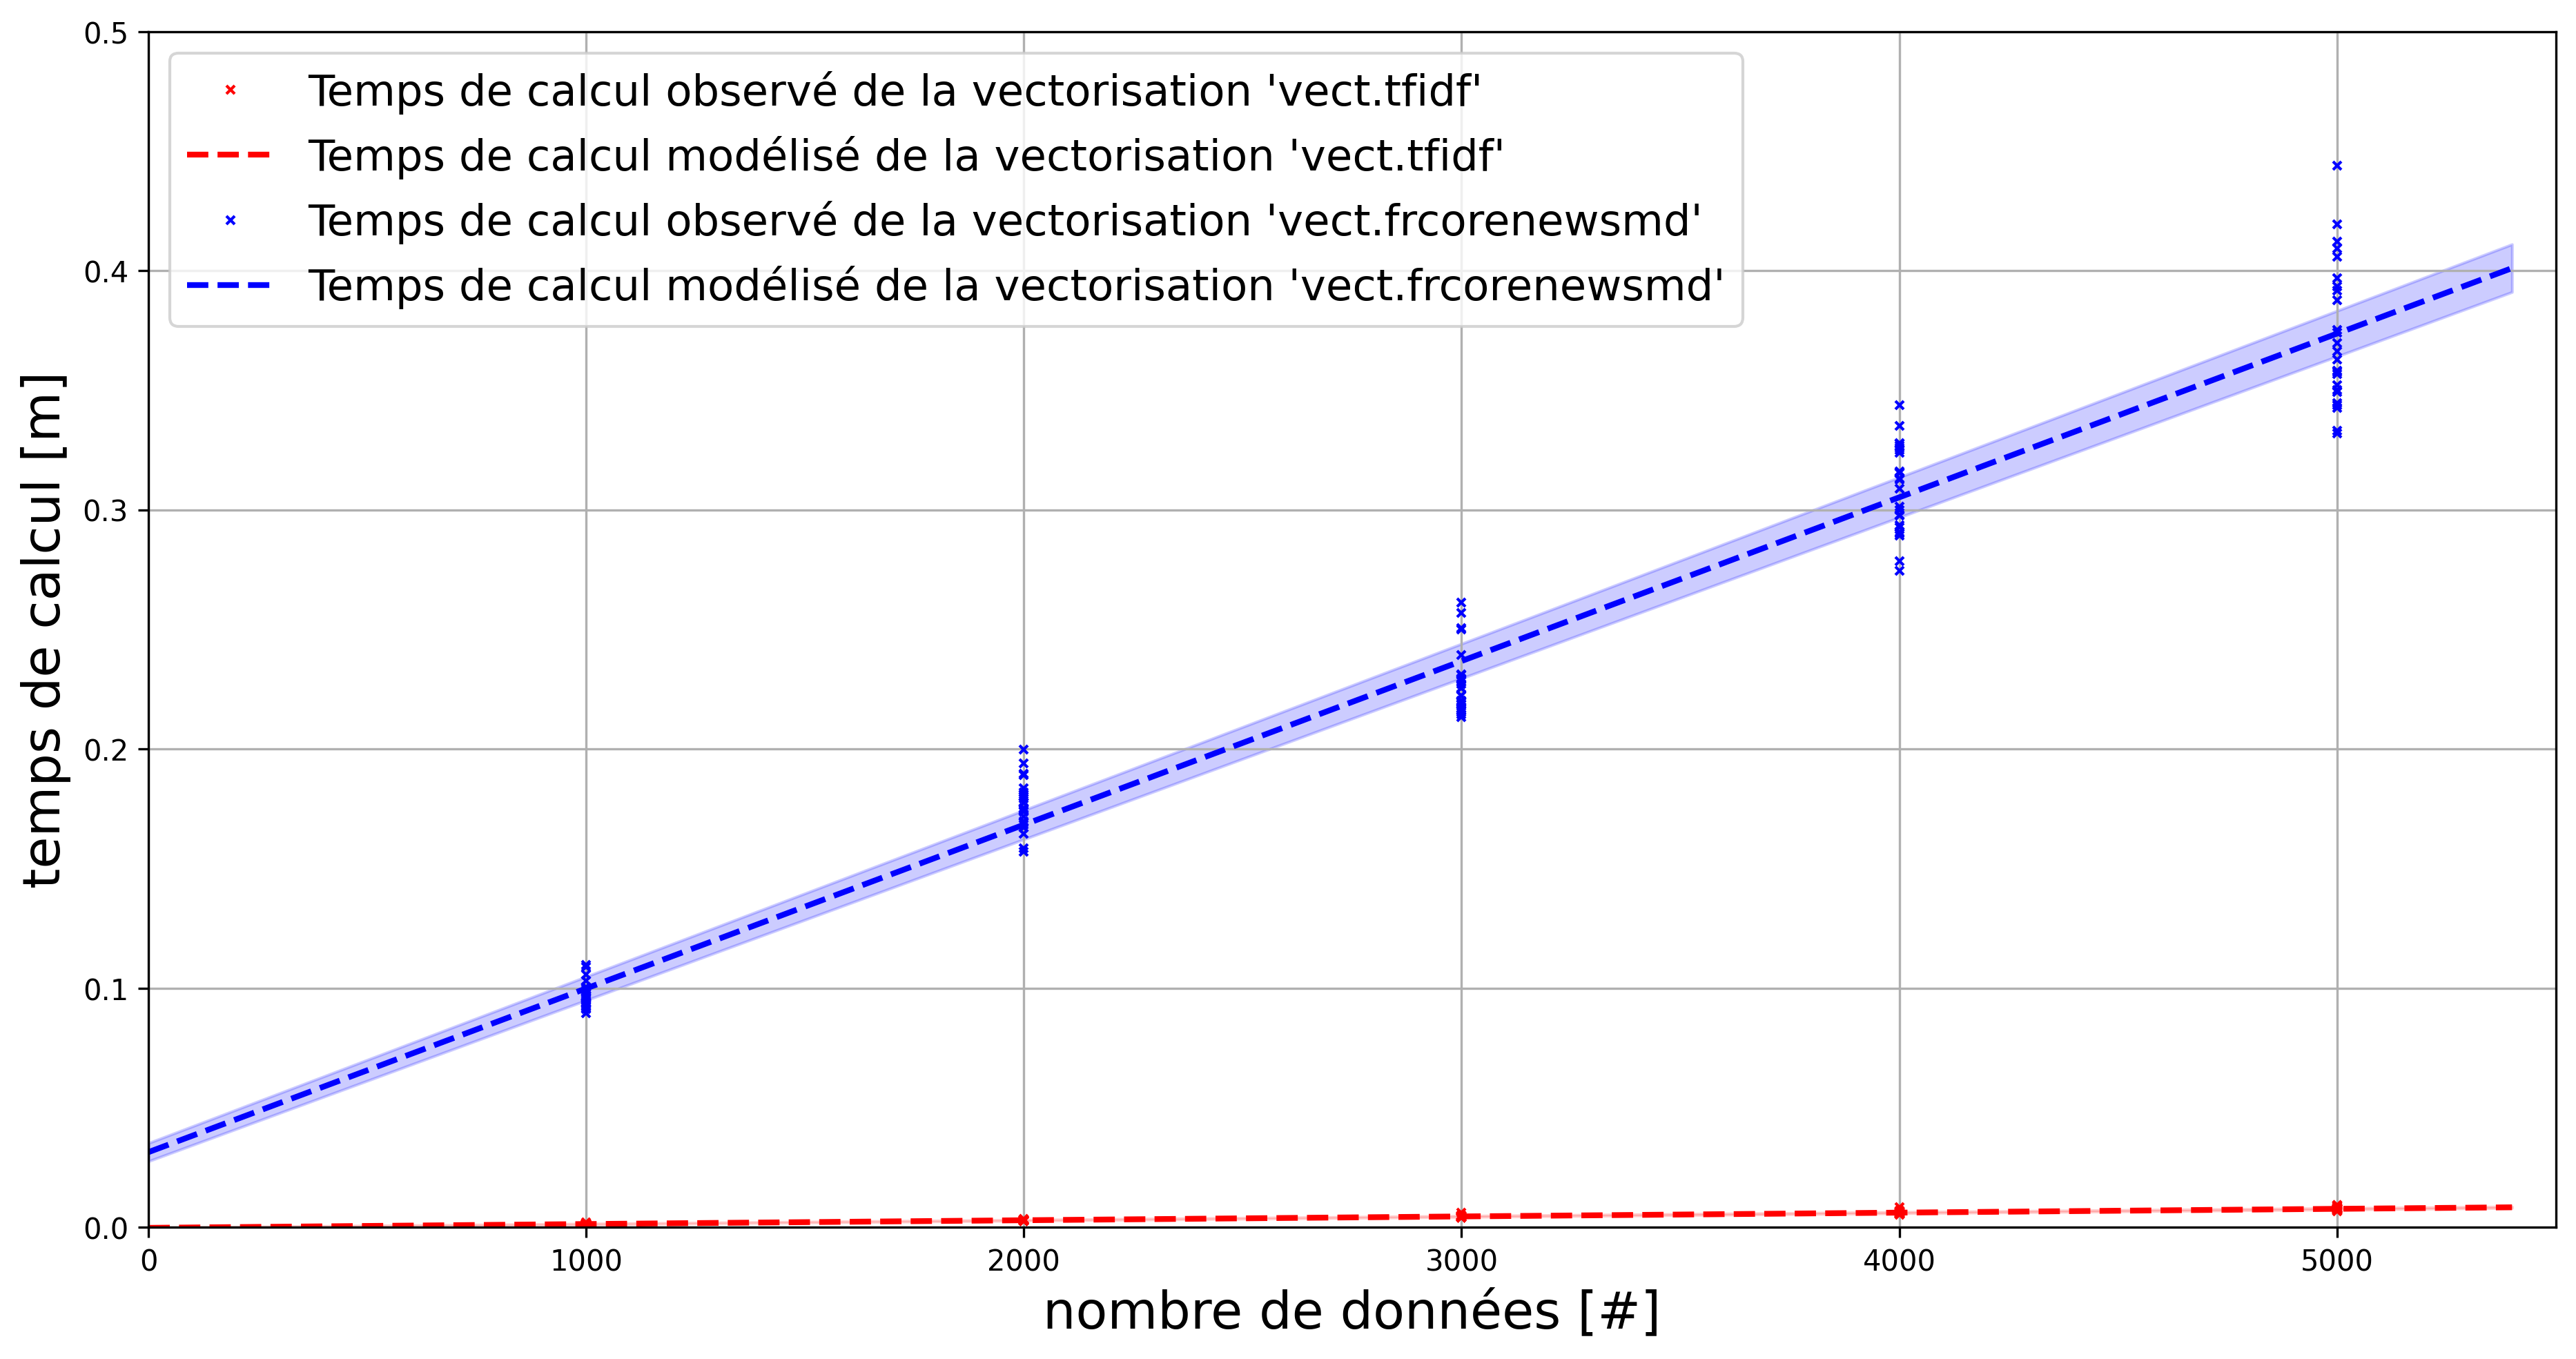
\includegraphics[width=0.95\textwidth]{figures/etude-temps-calcul-modelisation-2vect}
				\caption{
					Estimation du temps nécessaire (en minutes) pour effectuer une tâche de \textbf{vectorisation} en fonction du nombre de données à traiter.
				}
				\label{figure:4.3.2-ETUDE-COUTS-TEMPS-CALCUL-MODELISATION-VECTORIZATION}
			\end{figure}
			
			%%% Clustering
			
			% Première analyse.
			En ce qui concerne la tâche de \textbf{\textit{clustering} sous contraintes}, une première analyse montre que les modélisations des six implémentations sont différentiables (\texttt{p-valeur}: $<$ \texttt{$10^{-3}$}). Nous faisons donc une modélisation par algorithme.
			
			% Remarques: hiérarchique trop long.
			\begin{leftBarWarning}
				Plusieurs exécutions des algorithmes de type \textit{hiérarchique} ont été annulées pour les jeux données de tailles supérieures à $4~000$ car la durée excédé plusieurs heures.
				Nous limitons donc l'analyse de \texttt{clust.hier.sing}, \texttt{clust.hier.comp}, \texttt{clust.hier.avg} et \texttt{clust.hier.ward} aux tailles de $1~000$ à $3~000$.
			\end{leftBarWarning}
			
			% Modélisation du temps de calcul (clust.kmeans.cop).
			Pour les algorithmes du \textit{clustering} sous contraintes \texttt{clust.kmeans.cop}, l'analyse de la corrélation des facteurs avec les mesures de temps d'exécution indique qu'une modélisation minimale et suffisante peut être réalisée à partir du facteur $\texttt{dataset\_size}$ (\texttt{r}: $0.837$).
			Le second facteur le plus corrélé (mais non retenu) est l'interaction $\texttt{dataset\_size}^{\textbf{2}} \cdot \texttt{algorithm\_nb\_clusters}$ (\texttt{r}: $0.545$).
			Le modèle linéaire généralisé retenu (\texttt{R²}: $0.802$, \texttt{llf}: $-9.37 \cdot 10^{4}$, \texttt{llf\_null}: $-1.00 \cdot 10^{5}$) nous permet de déduire l'équation suivante :
			%
			\begin{equation}
				\texttt{computation\_time}(\texttt{clust.kmeans.cop})~[s]~
				\propto~1.45 \cdot 10^{-1} \cdot \texttt{dataset\_size}
			\end{equation}
			
			% Modélisation du temps de calcul (clust.hier.sing).
			Pour les algorithmes du \textit{clustering} sous contraintes \texttt{clust.hier.sing}, l'analyse de la corrélation des facteurs avec les mesures de temps d'exécution indique qu'une modélisation minimale et suffisante peut être réalisée à partir du facteur $\texttt{dataset\_size}^{\textbf{2}}$ (\texttt{r}: $0.940$).
			Le second facteur le plus corrélé (mais non retenu) est l'interaction $\texttt{dataset\_size}^{\textbf{2}} \cdot \texttt{algorithm\_nb\_clusters}$ (\texttt{r}: $0.729$).
			Le modèle linéaire généralisé retenu (\texttt{R²}: $0.987$, \texttt{llf}: $-5.54 \cdot 10^{4}$, \texttt{llf\_null}: $-6.10 \cdot 10^{4}$) nous permet de déduire l'équation suivante :
			%
			\begin{equation}
				\texttt{computation\_time}(\texttt{clust.hier.sing})~[s]~
				\propto~5.00 \cdot 10^{-4} \cdot \texttt{dataset\_size}^{\textbf{2}}
			\end{equation}
			
			% Modélisation du temps de calcul (clust.hier.comp).
			Pour les algorithmes du \textit{clustering} sous contraintes \texttt{clust.hier.comp}, l'analyse de la corrélation des facteurs avec les mesures de temps d'exécution indique qu'une modélisation minimale et suffisante peut être réalisée à partir du facteur $\texttt{dataset\_size}^{\textbf{2}}$ (\texttt{r}: $0.938$).
			Le second facteur le plus corrélé (mais non retenu) est l'interaction $\texttt{dataset\_size}^{\textbf{2}} \cdot \texttt{algorithm\_nb\_clusters}$ (\texttt{r}: $0.736$).
			Le modèle linéaire généralisé retenu (\texttt{R²}: $0.984$, \texttt{llf}: $-5.56 \cdot 10^{4}$, \texttt{llf\_null}: $-6.11 \cdot 10^{4}$) nous permet de déduire l'équation suivante :
			%
			\begin{equation}
				\texttt{computation\_time}(\texttt{clust.hier.comp})~[s]~
				\propto~4.99 \cdot 10^{-4} \cdot \texttt{dataset\_size}^{\textbf{2}}
			\end{equation}

			% Modélisation du temps de calcul (clust.hier.avg).
			Pour les algorithmes du \textit{clustering} sous contraintes \texttt{clust.hier.avg}, l'analyse de la corrélation des facteurs avec les mesures de temps d'exécution indique qu'une modélisation minimale et suffisante peut être réalisée à partir du facteur $\texttt{dataset\_size}^{\textbf{2}}$ (\texttt{r}: $0.915$).
			Le second facteur le plus corrélé (mais non retenu) est l'interaction $\texttt{dataset\_size}^{\textbf{2}} \cdot \texttt{algorithm\_nb\_clusters}$ (\texttt{r}: $0.713$).
			Le modèle linéaire généralisé retenu (\texttt{R²}: $0.981$, \texttt{llf}: $-5.90 \cdot 10^{4}$, \texttt{llf\_null}: $-6.45 \cdot 10^{4}$) nous permet de déduire l'équation suivante :
			%
			\begin{equation}
				\texttt{computation\_time}(\texttt{clust.hier.avg})~[s]~
				\propto~8.51 \cdot 10^{-4} \cdot \texttt{dataset\_size}^{\textbf{2}}
			\end{equation}

			% Modélisation du temps de calcul (clust.hier.ward).
			Pour les algorithmes du \textit{clustering} sous contraintes \texttt{clust.hier.ward}, l'analyse de la corrélation des facteurs avec les mesures de temps d'exécution indique qu'une modélisation minimale et suffisante peut être réalisée à partir du facteur $\texttt{dataset\_size}^{\textbf{2}}$ (\texttt{r}: $0.945$).
			Le second facteur le plus corrélé (mais non retenu) est l'interaction $\texttt{dataset\_size}^{\textbf{2}} \cdot \texttt{algorithm\_nb\_clusters}$ (\texttt{r}: $0.734$).
			Le modèle linéaire généralisé retenu (\texttt{R²}: $0.989$, \texttt{llf}: $-5.57 \cdot 10^{4}$, \texttt{llf\_null}: $-6.14 \cdot 10^{4}$) nous permet de déduire l'équation suivante :
			%
			\begin{equation}
				\texttt{computation\_time}(\texttt{clust.hier.ward})~[s]~
				\propto~5.30 \cdot 10^{-4} \cdot \texttt{dataset\_size}^{\textbf{2}}
			\end{equation}
			
			% Modélisation du temps de calcul (clust.spec).
			Pour les algorithmes du \textit{clustering} sous contraintes \texttt{clust.spec}, l'analyse de la corrélation des facteurs avec les mesures de temps d'exécution indique qu'une modélisation minimale et suffisante peut être réalisée à partir du facteur $\texttt{dataset\_size}^{\textbf{2}}$ (\texttt{r}: $0.658$).
			Le second facteur le plus corrélé (mais non retenu) est l'interaction $\texttt{dataset\_size}^{\textbf{2}} \cdot \texttt{algorithm\_nb\_clusters}$ (\texttt{r}: $0.595$).
			Le modèle linéaire généralisé retenu (\texttt{R²}: $0.527$, \texttt{llf}: $-7.89 \cdot 10^{5}$, \texttt{llf\_null}: $-8.27 \cdot 10^{5}$) nous permet de déduire l'équation suivante :
			%
			\begin{equation}
				\texttt{computation\_time}(\texttt{clust.spec})~[s]~
				\propto~8.18 \cdot 10^{-6} \cdot \texttt{dataset\_size}^{\textbf{2}}
			\end{equation}
			
			% Affichage du temps de calcul.
			La \textsc{Figure~\ref{figure:4.3.2-ETUDE-COUTS-TEMPS-CALCUL-MODELISATION-CLUSTERING}} représente ces modélisations de temps de calcul des algorithmes de \textit{clustering} en comparaison avec les mesures réalisées lors de l'expérience.
			\newline
			%
			\begin{figure}[!htb]
				\centering
				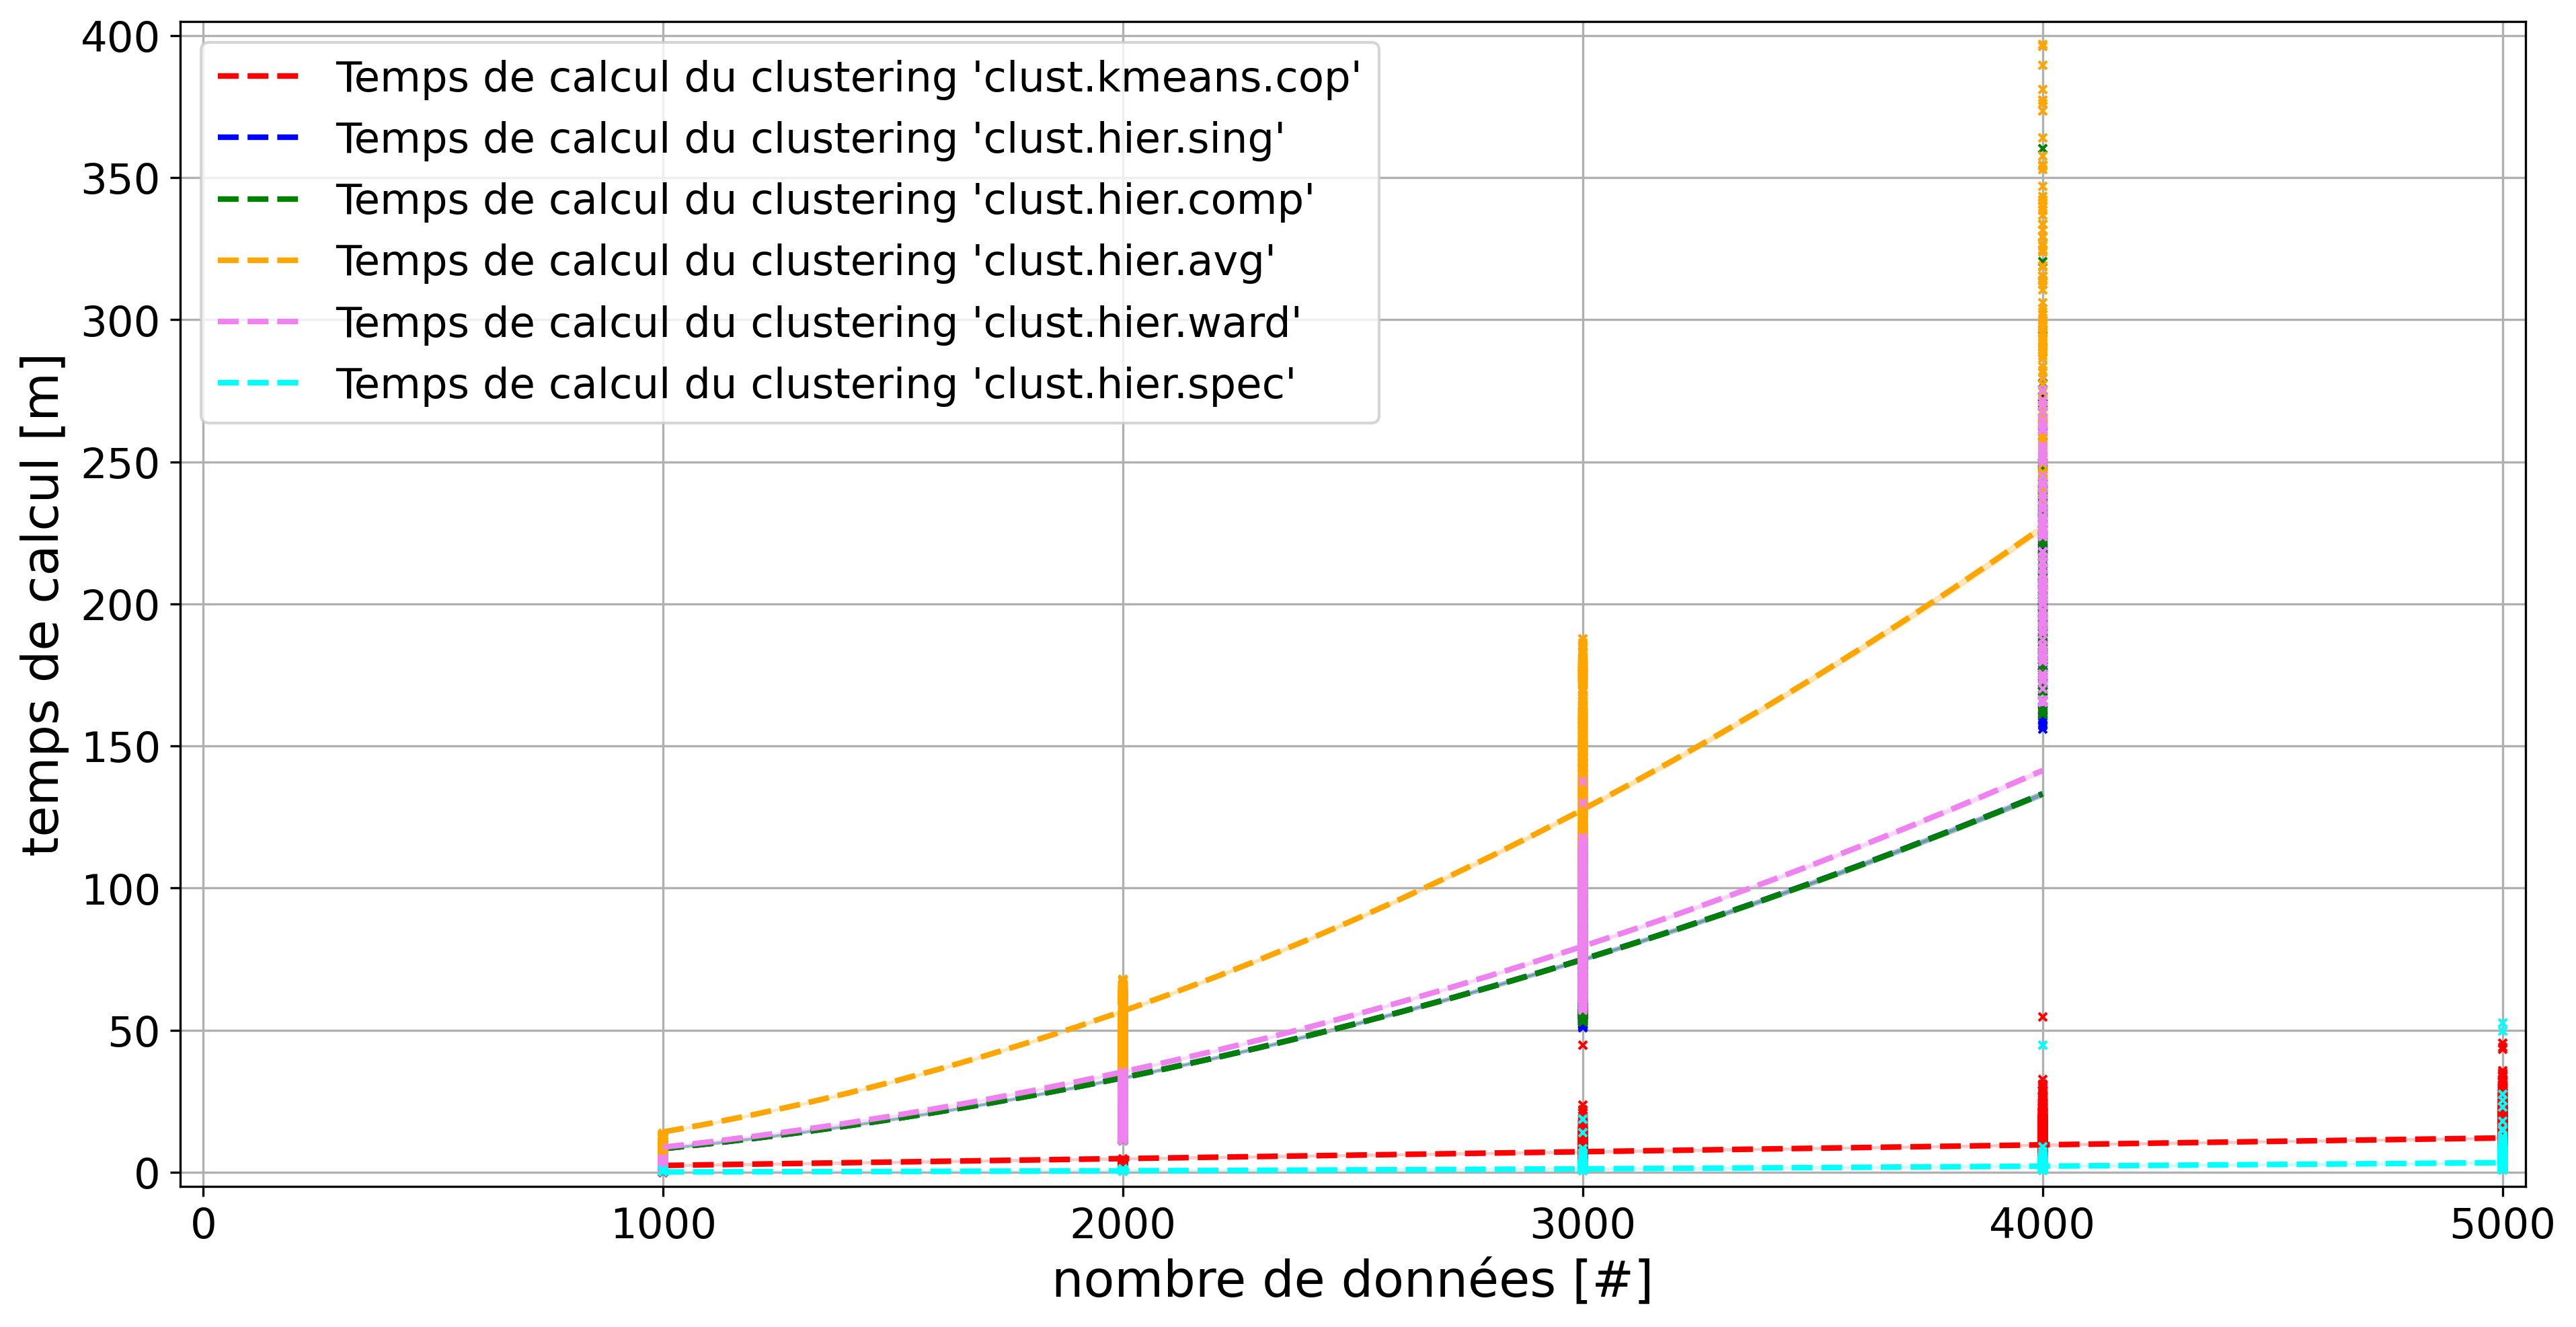
\includegraphics[width=0.95\textwidth]{figures/etude-temps-calcul-modelisation-3clust}
				\caption{
					Estimation du temps nécessaire (en minutes) pour effectuer une tâche de \textbf{clustering} en fonction du nombre de données à traiter.
				}
				\label{figure:4.3.2-ETUDE-COUTS-TEMPS-CALCUL-MODELISATION-CLUSTERING}
			\end{figure}
			
			%%% Sampling
			
			% Première analyse.
			En ce qui concerne la tâche d'\textbf{échantillonnage de contraintes}, une première analyse montre que les modélisations des quatre implémentations sont différentiables  (\texttt{p-valeur}: $<$ \texttt{$10^{-3}$}). Nous faisons donc une modélisation par algorithme.
			
			% Modélisation du temps de calcul (samp.rand.full).
			Pour les algorithmes de l'échantillonnage de contraintes \texttt{samp.rand.full}, l'analyse de la corrélation des facteurs avec les mesures de temps d'exécution indique qu'une modélisation minimale et suffisante peut être réalisée à partir du facteur $\texttt{dataset\_size}^{\textbf{2}}$ (\texttt{r}: $0.993$).
			Le second facteur le plus corrélé (mais non retenu) est l'interaction $\texttt{dataset\_size}^{\textbf{2}} \cdot \texttt{previous\_nb\_clusters}$ (\texttt{r}: $0.791$).
			Le modèle linéaire généralisé retenu (\texttt{R²}: $> 0.999$, \texttt{llf}: $-4.52 \cdot 10^{4}$, \texttt{llf\_null}: $-1.17 \cdot 10^{5}$) nous permet de déduire l'équation suivante :
			%
			\begin{equation}
				\texttt{computation\_time}(\texttt{samp.rand.full})~[s]~
				\propto~8.20 \cdot 10^{-7} \cdot \texttt{dataset\_size}^{\textbf{2}}
			\end{equation}
			
			% Modélisation du temps de calcul (samp.rand.same).
			Pour les algorithmes de l'échantillonnage de contraintes \texttt{samp.rand.same}, l'analyse de la corrélation des facteurs avec les mesures de temps d'exécution indique qu'une modélisation minimale et suffisante peut être réalisée à partir du facteur $\texttt{dataset\_size}^{\textbf{2}}$ (\texttt{r}: $0.939$).
			Le second facteur le plus corrélé (mais non retenu) est l'interaction $\texttt{dataset\_size}^{\textbf{2}} \cdot \texttt{algorithm\_nb\_constraints}$ (\texttt{r}: $0.611$).
			Le modèle linéaire généralisé retenu (\texttt{R²}: $> 0.999$, \texttt{llf}: $-3.20 \cdot 10^{4}$, \texttt{llf\_null}: $-6.84 \cdot 10^{4}$) nous permet de déduire l'équation suivante :
			%
			\begin{equation}
				\texttt{computation\_time}(\texttt{samp.rand.same})~[s]~
				\propto~1.85 \cdot 10^{-7} \cdot \texttt{dataset\_size}^{\textbf{2}}
			\end{equation}
			
			% Modélisation du temps de calcul (samp.farhtest.same).
			Pour les algorithmes de l'échantillonnage de contraintes \texttt{samp.farhtest.same}, l'analyse de la corrélation des facteurs avec les mesures de temps d'exécution indique qu'une modélisation minimale et suffisante peut être réalisée à partir du facteur $\texttt{dataset\_size}^{\textbf{2}}$ (\texttt{r}: $0.981$).
			Le second facteur le plus corrélé (mais non retenu) est l'interaction $\texttt{dataset\_size}^{\textbf{2}} \cdot \texttt{previous\_nb\_clusters}$ (\texttt{r}: $0.700$).
			Le modèle linéaire généralisé retenu (\texttt{R²}: $> 0.999$, \texttt{llf}: $-4.56 \cdot 10^{4}$, \texttt{llf\_null}: $-1.02 \cdot 10^{5}$) nous permet de déduire l'équation suivante :
			%
			\begin{equation}
				\texttt{computation\_time}(\texttt{samp.farhtest.same})~[s]~
				\propto~5.19 \cdot 10^{-7} \cdot \texttt{dataset\_size}^{\textbf{2}}
			\end{equation}
			
			% Modélisation du temps de calcul (samp.closest.diff).
			Pour les algorithmes de l'échantillonnage de contraintes \texttt{samp.closest.diff}, l'analyse de la corrélation des facteurs avec les mesures de temps d'exécution indique qu'une modélisation minimale et suffisante peut être réalisée à partir du facteur $\texttt{dataset\_size}^{\textbf{2}}$ (\texttt{r}: $0.995$).
			Le second facteur le plus corrélé (mais non retenu) est l'interaction $\texttt{dataset\_size}^{\textbf{2}} \cdot \texttt{previous\_nb\_clusters}$ (\texttt{r}: $0.815$).
			Le modèle linéaire généralisé retenu (\texttt{R²}: $> 0.999$, \texttt{llf}: $-5.96 \cdot 10^{4}$, \texttt{llf\_null}: $-1.36 \cdot 10^{5}$) nous permet de déduire l'équation suivante :
			%
			\begin{equation}
				\texttt{computation\_time}(\texttt{samp.closest.diff})~[s]~
				\propto~1.43 \cdot 10^{-6} \cdot \texttt{dataset\_size}^{\textbf{2}}
			\end{equation}
			
			% Affichage du temps de calcul.
			La \textsc{Figure~\ref{figure:4.3.2-ETUDE-COUTS-TEMPS-CALCUL-MODELISATION-SAMPLING}} représente ces modélisations de temps de calcul des algorithmes d'échantillonnage en comparaison avec les mesures réalisées lors de l'expérience.
			\newline
			%
			\begin{figure}[!htb]
				\centering
				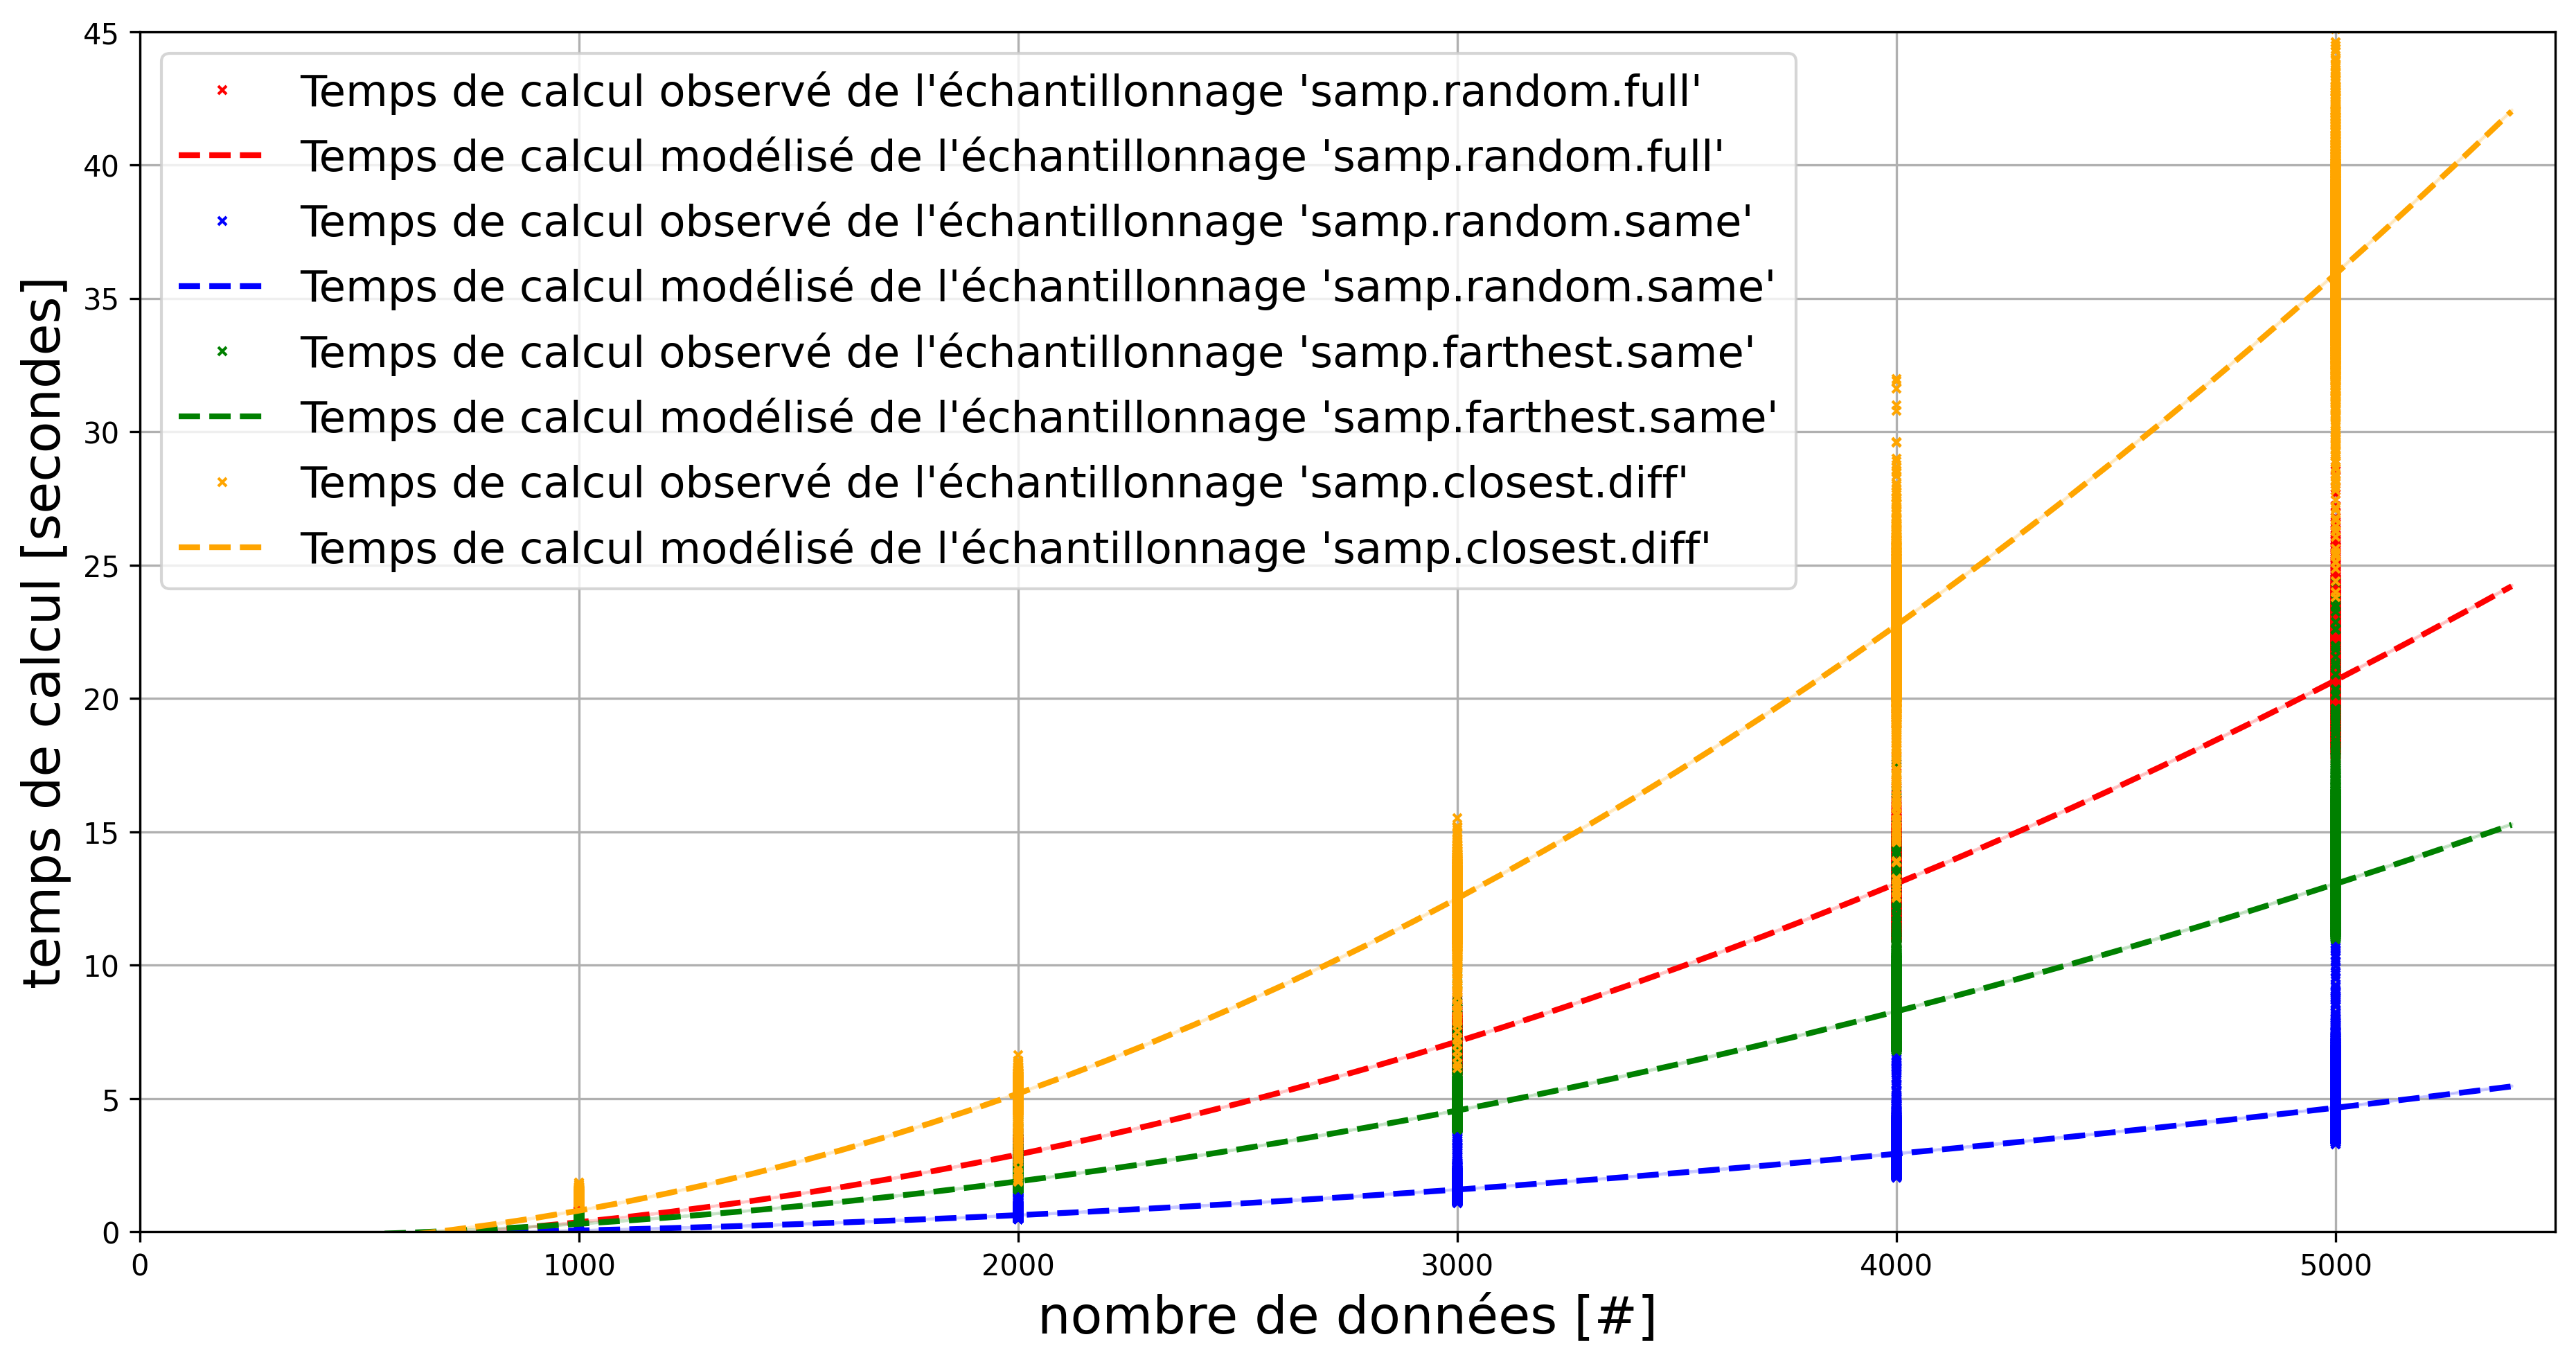
\includegraphics[width=0.95\textwidth]{figures/etude-temps-calcul-modelisation-4samp}
				\caption{
					Estimation du temps nécessaire (en minutes) pour effectuer une tâche d'\textbf{échantillonnage de contraintes} en fonction du nombre de données à traiter.
				}
				\label{figure:4.3.2-ETUDE-COUTS-TEMPS-CALCUL-MODELISATION-SAMPLING}
			\end{figure}

		%%% Discussion.
		\subsubsection{Discussion}
		
			% Rappel de l'objectif : estimer le temps d'exécution.
			Dans cette étude, nous avons estimé le temps de calcul des différents algorithmes implémentés afin de confirmer le choix de paramétrage pour une convergence optimal (cf. hypothèse d'efficience en \textsc{Section~\ref{section:4.2-HYPOTHESE-EFFICIENCE}}).
			Ces estimations ont été réalisées sur la base de plusieurs exécutions et fonction de divers contextes d'utilisation : nombre de données, nombre de contraintes annotées, nombre de contraintes à sélectionner, nombre de \textit{clusters} existant, nombre de \textit{clusters} à trouver.
			\\
			
			% Remarque générale : Dépend principalement du nombre de données.
			En premier lieu, on peut constater que les différentes modélisations dépendent majoritairement de la taille du jeu de données manipulé ($\texttt{dataset\_size}$ ou $\texttt{dataset\_size}^{\textbf{2}}$) avec un score de corrélation \texttt{r} avec le temps mesuré généralement supérieur à $0.9$ et des modèles \textit{GLM} avec des coefficients de détermination généralisé \texttt{R²} généralement proches de $0.999$.
			Bien que d'autres facteurs peuvent intervenir dans ces estimations (notamment les interactions doubles entre la taille du jeu de données et le nombre de \textit{clusters} ou le nombre de contraintes), ces derniers semblent avoir un impact négligeable sur le temps d'exécution.
			
			% Note: remarque sur le nombre de contraintes.
			\begin{leftBarAuthorOpinion}
				Certains paramétrages de la méthode du \textit{clustering} interactif semblent cependant avoir un temps de calcul décroissant au cours des itérations, mais nous n'avons cependant pas pu montrer de tendances globales significatives.
				Il est probable que l'ajout de contraintes judicieusement placées permettent à certains algorithmes de \textit{clustering} de s'exécuter plus rapidement, notamment lorsque ceux-ci exploitent les composants connexes du graphe de contraintes (cf. \textsc{Section~\ref{section:3.3.2-GESTION-DES-CONTRAINTES}}). En effet, :
				\begin{itemize}
					\item les \textit{clustering} hiérarchiques s'initialisent autant de \textit{clusters} que de groupes de données liées entre elles par des contraintes \texttt{MUST-LINK} : or s'il y a plus de contraintes, alors les composants connexes sont davantage développés, donc il y a moins de \textit{clusters} à initialiser et donc moins d'époques de l'algorithme ;
					\item le \textit{clustering} KMeans (modèle COP) attire auprès d'un barycentre l'ensemble des données liées par un \texttt{MUST-LINK} : or s'il y a plus de contraintes, alors il y a des données attirées, donc les noyaux de \textit{clusters} peuvent se stabiliser plus rapidement.  
				\end{itemize}
				Toutefois, ces suppositions n'ont pas pu être démontrées, et certains contre-exemples tendent à conclure que ces comportements sont très dépendants du jeu de données manipulé et de l'ordre d'ajout des contraintes. Par exemple :
				\begin{itemize}
					\item l'ajout d'un trop grand nombre de contraintes \texttt{CANNOT-LINK} peut engendrer un surplus de vérification pour estimer quelles formations de \textit{clusters} sont autorisées sans violer de contraintes ;
					\item l'algorithme KMeans (modèle COP) peut osciller autour de plusieurs noyaux de \textit{clusters} instables si les contraintes violent trop la similarité intrinsèque des données.
				\end{itemize}
			\end{leftBarAuthorOpinion}
			
			% Cas du clustering.
			En ce qui concerne la tâche de \textit{clustering}, on note des différences significatives dans les temps d'exécution des divers algorithmes implémentés.
			En effet, l'algorithme KMeans (modèle COP) est nettement plus rapide (complexité estimée en $ \mathcal{O}(\texttt{dataset\_size}) $, nécessitant quelques dizaines de minutes pour $5~000$ données) que les implémentations du \textit{clustering} hiérarchique (complexité estimée en $ \mathcal{O}(\texttt{dataset\_size}^{\textbf{2}}) $, nécessitant plusieurs heures dès $3~000$ données).
			Cette différence, visible en \textsc{Figure~\ref{figure:4.3.2-ETUDE-COUTS-TEMPS-CALCUL-MODELISATION-CLUSTERING}}, a un réel impact sur l'expérience utilisateur de l'opérateur.
			En effet, bien qu'il soit théoriquement plus efficient pour atteindre une annotation suffisante (cf. hypothèse d'efficience en \textsc{Section~\ref{section:4.2-HYPOTHESE-EFFICIENCE}}), l'usage d'un \textit{clustering} hiérarchique imposerait de longs temps d'attente à l'opérateur, interdisant des interactions rapides avec la machines.
			Or l'intérêt principal de notre méthodologie d'annotation à l'aide du \textit{clustering} interactif repose sur ces interactions homme-machine via l'ajout régulier de contraintes pertinentes (cf. hypothèse d'efficacité en \textsc{Section~\ref{section:4.1-HYPOTHESE-EFFICACITE}}).
			Nous décidons donc d'exclure l'usage des algorithmes de \textit{clustering} hiérarchique au profit du \textit{clustering} KMeans (modèle COP).
			
			% Note: Cas du projet étudiant avec TPS.
			\begin{leftBarInformation}
				Dans le cadre du projet étudiant avec l'école Télécom Physique Strasbourg visant à implémenter d'autres algorithmes de \textit{clustering} sous contraintes, un résonnement similaire a été utilisé pour filtrer les algorithmes. Ainsi, l'implémentation de KMeans (modèle MPC) a été exclu (complexité estimée en $ \mathcal{O}(\texttt{dataset\_size}^{\textbf{3}}) $) et l'implémentation de la propagation par affinité écarte la gestion des contraintes \texttt{CANNOT-LINK} pour avoir un temps d'exécution comparable au \textit{clustering} KMeans (modèle COP). L'algorithme DBScan (modèle C-DBScan) est quand à lui un rival possible avec une complexité estimée en $ \mathcal{O}(\texttt{dataset\_size}) $.
			\end{leftBarInformation}
			
			% Cas du prétraitement + vectorisation + échantillonnage.
			En ce qui concerne les tâches de prétraitements (cf. \textsc{Figure~\ref{figure:4.3.2-ETUDE-COUTS-TEMPS-CALCUL-MODELISATION-PREPROCESSING}}), de vectorisation (cf. \textsc{Figure~\ref{figure:4.3.2-ETUDE-COUTS-TEMPS-CALCUL-MODELISATION-VECTORIZATION}}), et d'échantillonnage de contraintes (cf. \textsc{Figure~\ref{figure:4.3.2-ETUDE-COUTS-TEMPS-CALCUL-MODELISATION-SAMPLING}}) ont des complexités presque négligeables en représentant moins de $10$\% des temps d'exécution du \textit{clustering} (pour $5~000$ données : moins de $1$ minute pour les trois algorithmes, contre $12.1$ minutes pour \texttt{clust.kmeans.cop} et $3.5$ heures pour \texttt{clust.hier.sing}).
			Nous maintenons donc les paramétrages obtenus pour ces tâches en \textsc{Section~\ref{section:4.2-HYPOTHESE-EFFICIENCE}} sans analyses complémentaires, et nous utilisons l'estimation temporelle du \textit{clustering} \texttt{clust.kmeans.cop} majorée de $10$\%.
			
			% Conclusion.
			\begin{leftBarSummary}
				Dans l'optique d'atteindre de manière efficiente $90$\% de \texttt{v-measure}\footnote{
					$90$\% de \texttt{v-measure}: cas d'une annotation dite partielle, dont le paramétrage le plus efficient est constitué du prétraitement simple (\texttt{prep.simple}), de la vectorisation TF-IDF (\texttt{vect.tfidf}), du \textit{clustering} hiérarchique à lien moyen (\texttt{clust.hier.avg}) et de l'échantillonnage des données les plus proches dans des clusters différents (\texttt{sampl.closest.diff})
				}
				avec un coût global minimal, nous retenons l'usage du \textbf{paramétrage favori} constitué du prétraitement simple (\texttt{prep.simple}), de la vectorisation TF-IDF (\texttt{vect.tfidf}), du \textit{clustering} KMeans avec modèle COP (\texttt{clust.kmeans.cop}) et de l'échantillonnage des données les plus proches dans des clusters différents (\texttt{sampl.closest.diff}).
				On estime le temps d'exécution de ce paramétrage avec l'équation suivante\footnote{
					Temps du paramétrage favori : environ $2.8$ minutes pour $1~000$ données ; environ $14.2$ minutes pour $5~000$ données.
				} :
				%
				\begin{equation}
					\label{equation:4.3.2-ETUDE-COUTS-TEMPS-CALCUL-PARAMETRAGE-FAVORI}
					\texttt{computation\_time}(\texttt{settings.favorite})~[s]~
					\propto~0.17 \cdot \texttt{dataset\_size}
				\end{equation}
			\end{leftBarSummary}
	
	%%%
	%%% Subsection 4.3.3: Étude du nombre de contraintes nécessaires à la convergence vers une vérité terrain pré-établie en fonction de la taille du jeu de données 
	%%%
	\subsection{Étude du nombre de contraintes nécessaires à la convergence vers une vérité terrain pré-établie en fonction de la taille du jeu de données}
	\label{section:4.3.3-ETUDE-COUT-NOMBRE-CONTRAINTES}
			
		% Transition.
		Avec les deux précédentes études, nous sommes capable d'estimer le temps nécessaire à un expert pour annoter des contraintes et le temps nécessaire à la machine pour proposer un nouveau \textit{clustering} adapté aux suggestions de l'expert.
		Pour poursuivre nos études et pouvoir estimer le coût total d'un projet d'annotation, il nous reste à estimer le nombre total de contraintes à devoir renseigner en fonction de la taille du jeu de données.
		
		% Objectif de l'expérience.
		Pour cela, nous allons simuler la création de cette base d'apprentissage en adaptant le protocole utilisé lors de notre étude d'efficacité (cf. \textsc{Section~\ref{section:4.1.1-ETUDE-CONVERGENCE}}) :
		nous employons notre méthode de \textit{clustering} interactif avec notre \textbf{paramétrage favori}\footnote{
			Paramétrage favori (atteindre $90$\% de \texttt{v-measure} avec un coût minimal): prétraitement simple (\texttt{prep.simple}), vectorisation TF-IDF (\texttt{vect.tfidf}), \textit{clustering} KMeans avec modèle COP (\texttt{clust.kmeans.cop}) et échantillonnage des données les plus proches dans des clusters différents (\texttt{sampl.closest.diff})
		}
		sur des jeux de données de différentes tailles et mesurons le nombre de contraintes nécessaires pour converger vers la vérité terrain.
	
		%%% Protocole expérimental.
		\subsubsection{Protocole expérimental}
			
			% Axiome.
			\begin{leftBarWarning}
				Dans le cadre de cette étude, nous supposons que l'expert métier connaît parfaitement le domaine traité dans ce jeu de données, et qu'il est capable de caractériser sans ambiguïté la similitude entre deux données issues de cet ensemble.
			\end{leftBarWarning}
			
			% Pseudo-code.
			Pour résumer le protocole expérimental que nous décrivons ci-dessous, vous pouvez vous référer au pseudo-code décrit dans \textsc{Algorithme~\ref{algorithm:4.3.3-ETUDE-COUT-NOMBRE-CONTRAINTES-PROTOCOLE}}.
			
			\begin{algorithm}
				\KwData{jeux de données annotées (vérités terrains) de tailles différentes}
				%
				\ForEach{jeux de données à tester}{
					\textbf{initialisation (données)}: récupérer ou générer les données et la vérité terrain \;
					\textbf{initialisation (contraintes)}: créer une liste vide de contraintes \;
					\textbf{prétraitement}: supprimer le bruit dans les données avec \texttt{prep.simple} \;
					\textbf{vectorisation}: transformer les données en vecteurs avec \texttt{vect.tfidf} \;
					\textbf{clustering initial}: regrouper les données par similarité avec \texttt{clust.kmeans.cop} \;
					\textbf{évaluation}: estimer l'équivalence entre le \textit{clustering} et la vérité terrain \;
					\Repeat{annotation de toutes les contraintes possibles}{
						\textbf{échantillonnage}: sélectionner des contraintes avec \texttt{samp.closest.diff} \;
						\textbf{simulation d'annotation}: déterminer les contraintes avec la vérité terrain \;
						\textbf{intégration}: ajouter les nouvelles contraintes au gestionnaire de contraintes \;
						\textbf{clustering}: regrouper les données par similarité avec \texttt{clust.kmeans.cop} \;
						\textbf{évaluation}: estimer l'équivalence entre le \textit{clustering} et la vérité terrain \;
					}
				}
				\textbf{analyse}: entraîner un modèle linéaire généralisé du nombre de contraintes nécessaires \;
				%
				\KwResult{modélisation du nombre de contraintes nécessaires pour un jeu de données}
				%
				\caption{\textit{
					Description en pseudo-code du protocole expérimental de l'étude du nombre de contraintes nécessaires pour converger vers une vérité terrain pré-établie avec notre paramétrage favori du \textit{clustering} interactif.
				}}
				\label{algorithm:4.3.3-ETUDE-COUT-NOMBRE-CONTRAINTES-PROTOCOLE}
			\end{algorithm}
			
			% Description des jeux de données.
			Nous utilisons deux vérités terrains comme références pour cette expérience :
			\begin{itemize}
				% Bank Cards.
				\item le jeu de données \texttt{Bank Cards (v2.0.0)} :
				ce dernier traite des demandes les plus fréquentes des clients en ce qui concerne la gestion de leur carte bancaire.
				Il est composé de $1~000$ questions rédigées en français et réparties en $10$ classes (\texttt{perte ou vol de carte}, \texttt{carte avalée}, \texttt{commande de carte}, ...).
				Pour plus de détails, consultez l'annexe~\ref{annex:A.1-DATASET-BANK-CARDS} ;
				% MLSUM.
				\item le jeu de données \texttt{MLSUM FR Train Subset (v1.0.0-schild)} :
				ce dernier concerne les titres d'articles de journaux issus des catégories de publication les plus communes.
				Il est composé de $744$  titres d'articles rédigés et répartis en $14$ classes (\textit{économie}, \textit{sport}, ...).
				Pour plus de détails, consultez l'annexe~\ref{annex:A.2-DATASET-MLSUM-SUBSET-SCHILD} ;
			\end{itemize}

			Cependant, deux jeux de données ne nous permettent pas d'analyser l'impact du nombre de données sur le nombre de contraintes nécessaires pour converger vers une vérité terrain.
			Pour utiliser facilement plusieurs jeux de données de tailles différentes tout en maîtrisant leur contenu, nous avons donc dupliqué aléatoirement des données issues de ces jeux de référence en y insérant des fautes de frappes.
			La taille des jeux de données générés, notée $\texttt{dataset\_size}$, varie entre $1~000$ à $5~000$ par pas de $250$, et chaque taille de jeu est générée $3$ fois pour contrer les aléas statistiques de création.
			Il y a donc $51$ variations de chaque jeu de références, soit $102$ jeux utilisés de tailles différentes.
			
			% Remarque.
			\begin{leftBarWarning}
				Dans le cadre de cette étude, nous faisons l'hypothèse que cette création artificielle de données n'a pas d'impact majeur sur le nombre de contraintes nécessaires pour converger vers une vérité terrain.
			\end{leftBarWarning}
			
			% Description des tentatives de la méthode.
			Sur chacun de ces jeux générés, une tentative complète\footnote{
				Tentative complète : itérations d'échantillonnage, d'annotation et de \textit{clustering} jusqu'à annotation de toutes les contraintes possibles.
			}
			de la méthode du \textit{clustering} interactif en utilisant notre paramétrage favori est exécuté, et chaque tentative est répétée $5$ fois pour contrer les aléas statistiques des exécutions.
			Il y a donc $510$ tentatives de \textit{clustering} interactif réalisées.
			
			% Description de l'évaluation.
			Pour chacune de ces tentatives, nous nous intéressons au nombre de contraintes nécessaires pour atteindre le seuil d'annotation partielle (caractérisé par $90$\% de \texttt{v-measure} entre la vérité terrain et la segmentation des données obtenue), et nous entraînons un modèle linéaire généralisé (\textit{GLM}) pour modéliser le nombre de contraintes requis en fonction de la taille du jeu de données (noté $\texttt{dataset\_size}$).
			Ce modèle sera caractérisé par le coefficient de détermination généralisé \texttt{R²} de \textit{Cox et Snel} (\cite{diamond-etal:1990:analysis-binary-data}), la log-vraisemblance \texttt{llf} (\cite{edwards:1992:likelihood}) et la log-vraisemblance \texttt{llf\_null} du modèle \textit{null}.
			Pour finir, nous discutons des valeurs des coefficients obtenus sur l'impact du nombre d'itérations de la méthode à prévoir.

			% Référence scripts.
			\begin{leftBarInformation}
				Les scripts de l'expérience, réalisés avec des \textit{notebooks} Python (\cite{van-rossum-drake:2009:python-reference-manual}), sont disponibles dans un dossier dédié de~\cite{schild:2021:cognitivefactory-interactiveclusteringcomparativestudy}.
				Nous utilisons entre autres la librairie \texttt{statsmodels} (\cite{seabold-perktold:2010:statsmodels-econometric-statistical}).
			\end{leftBarInformation}

		%%% Résultats.
		\subsubsection{Résultats obtenus}
		
			% Modélisation du nombre de contraintes.
			Le modèle linéaire généralisé entraîné sur les mesures du nombre de contraintes requis pour atteindre $90$\% de \texttt{v-measure} (\texttt{R²}: $> 0.999$, \texttt{llf}: $-4~327.6$, \texttt{llf\_null}: $-4~942.9$) nous permet de déduire l'équation suivante :
			%
			\begin{equation}
				\label{equation:4.3.3-ETUDE-COUT-NOMBRE-CONTRAINTES}
				\texttt{constraints\_needed}(\texttt{settings.favorite})~[\#]~
				\propto~3.15 \cdot \texttt{dataset\_size}
			\end{equation}
			%
			La \textsc{Figure~\ref{figure:4.3.3-ETUDE-COUT-NOMBRE-CONTRAINTES}} représente cette modélisation.
			\newline
			%
			\begin{figure}[!htb]
				\centering
				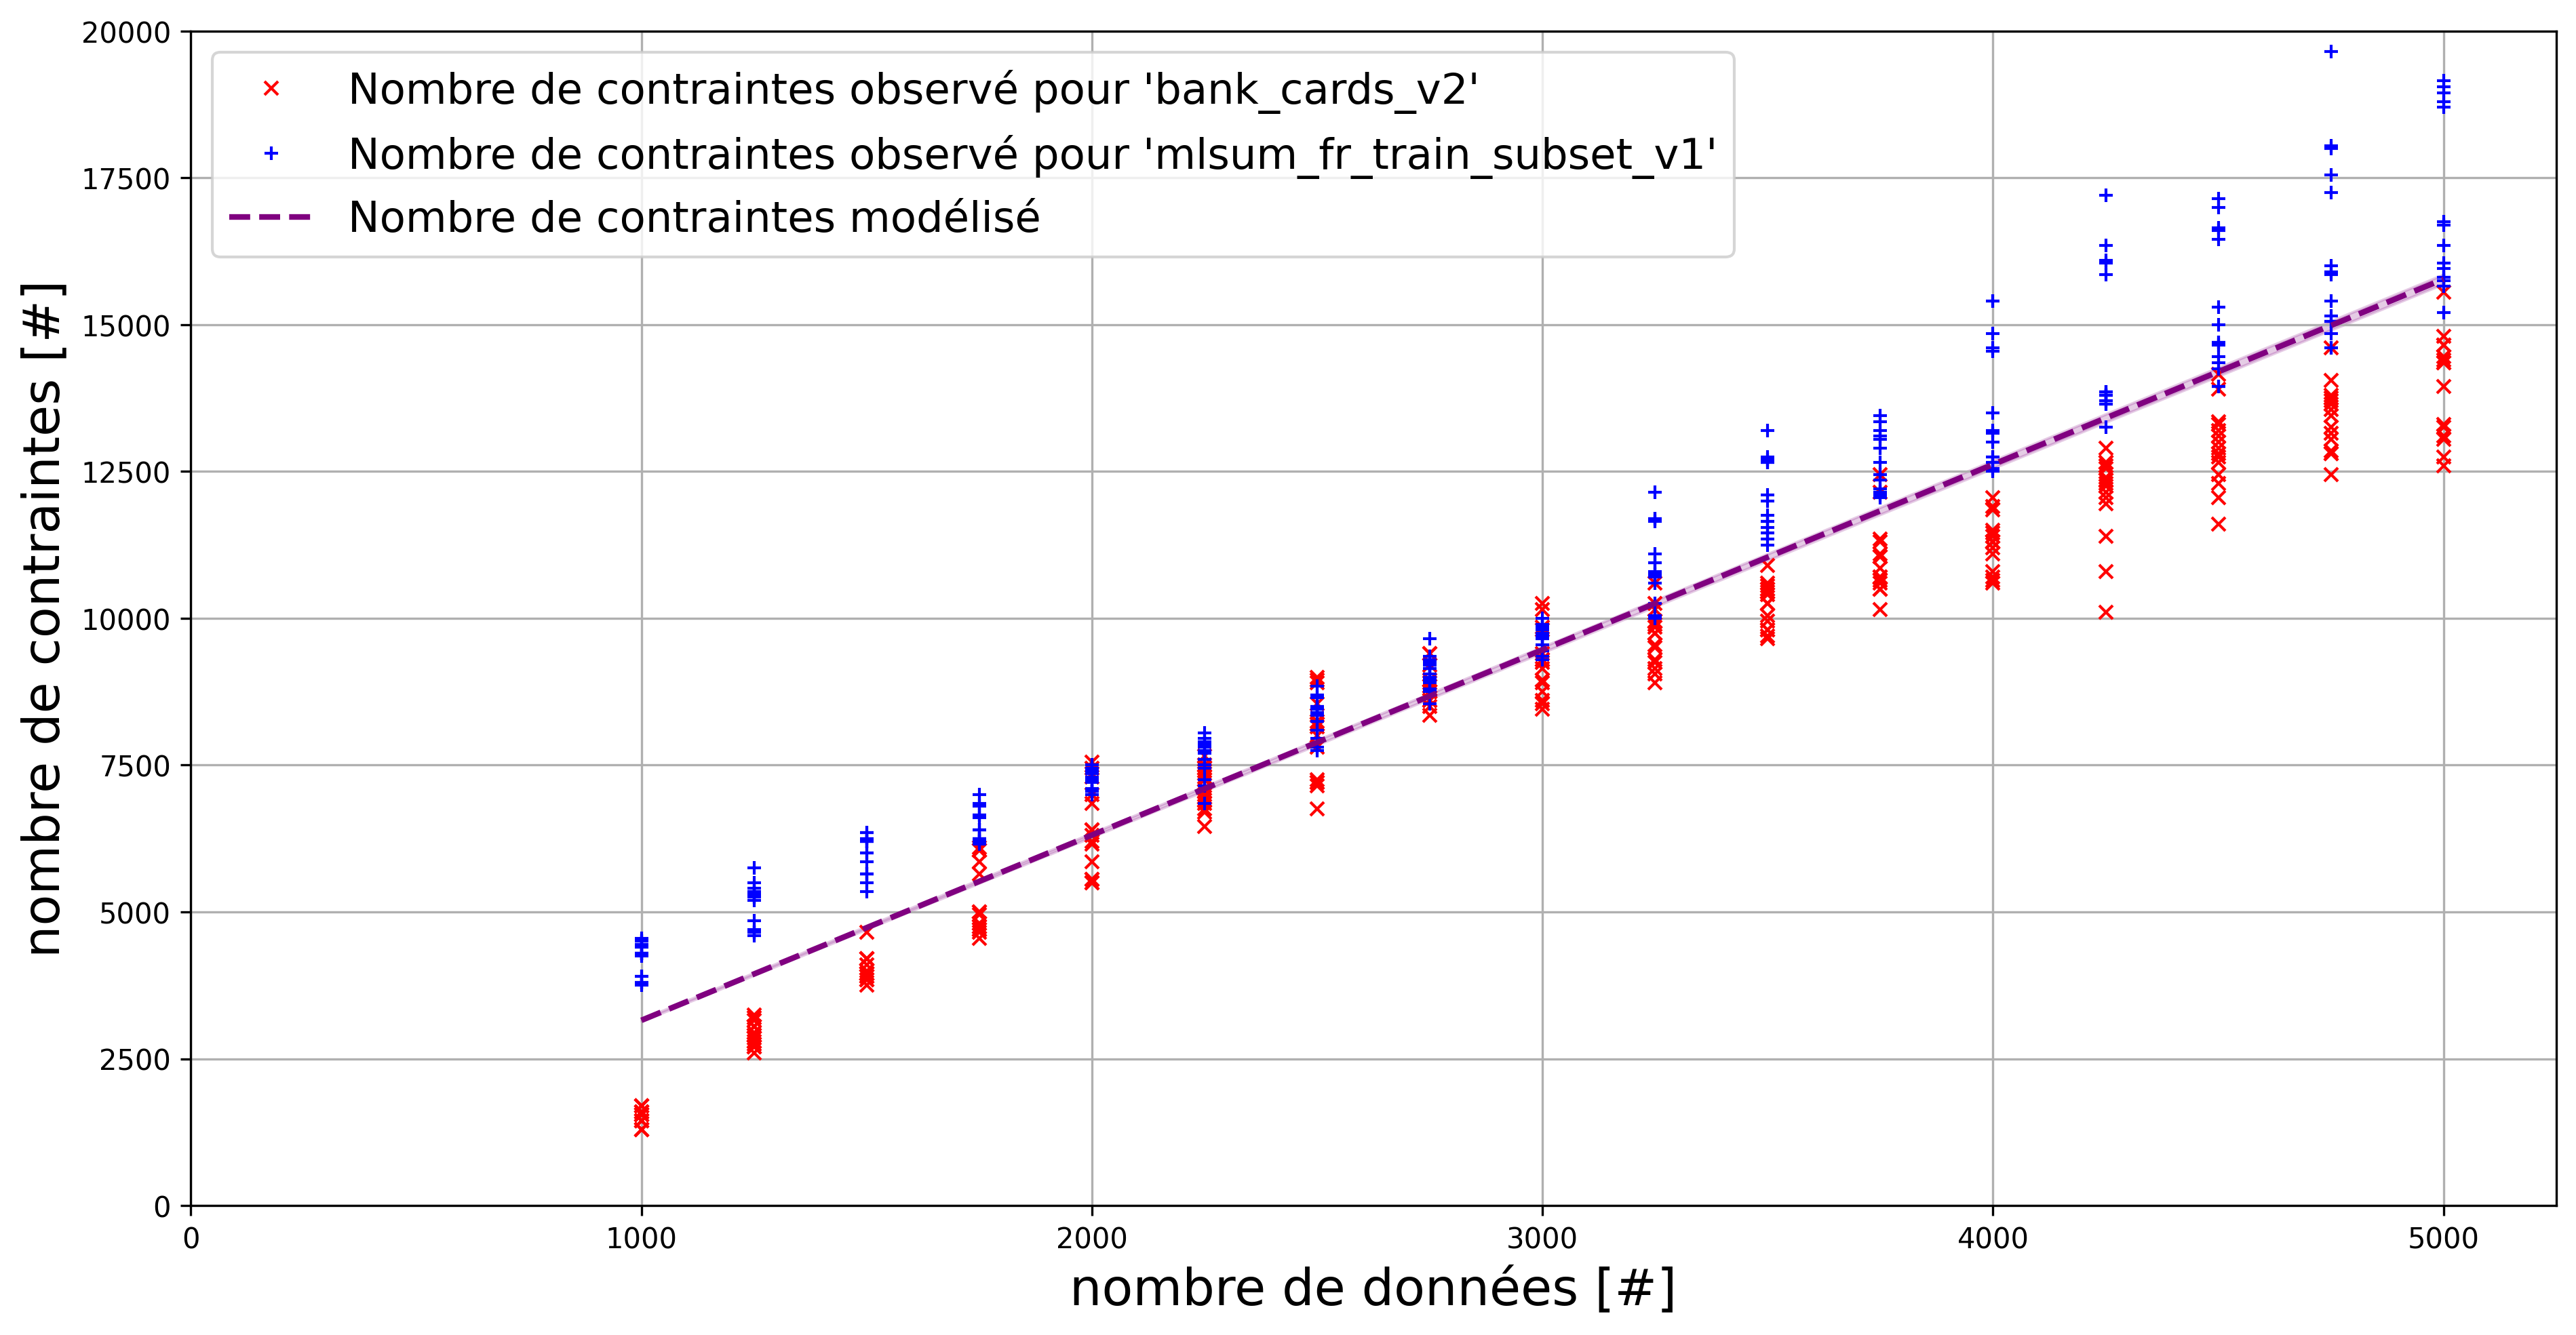
\includegraphics[width=0.95\textwidth]{figures/etude-nombre-contraintes-1-modelisation-nombre}
				\caption{
					Estimation du nombre moyen de contraintes nécessaire à notre \textbf{paramétrage favori} du \textit{clustering} interactif afin d'obtenir une annotation partielle (\textit{atteindre une \texttt{v-measure} de $90$\%}) en fonction de la taille du jeu de données à modéliser.
				}
				\label{figure:4.3.3-ETUDE-COUT-NOMBRE-CONTRAINTES}
			\end{figure}
		
			% Note de l'auteur.
			\begin{leftBarAuthorOpinion}
				% Estimation de points de références.
				On peut considérer les points de références suivants :
				\begin{itemize}
					\item le nombre de contraintes possibles (avec doublons) est de $\texttt{dataset\_size}^{\textbf{2}}$ (\textit{caractériser chaque couple de données présent dans la matrice d'adjacence}) ;
					\item le nombre de contraintes possibles (sans doublons) est de $\frac{1}{2} \cdot (\texttt{dataset\_size}^{\textbf{2}} - \texttt{dataset\_size})$ (\textit{considérer la symétrie des contraintes, donc seul le triangle supérieur de la matrice d'adjacence a besoin d'être renseigné}) ;
					\item le nombre minimal de contraintes à annoter pour être exhaustif sur une partition en $k$ \textit{clusters} $\{K_{1}, K_{2}, ..., K_{k}\} $ est estimé à ${\displaystyle \sum\limits_{1 \leq i \leq k}{(\|K_{i}\|-1)} + \sum\limits_{1 \leq i \leq k}{(k-i)}} $
					(\textit{il faut d'abord considérer les chemins minimaux pour parcourir les composants connexes avec des contraintes \texttt{MUST-LINK}, correspondant à $\|K_{i}\|-1$ contraintes \texttt{MUST-LINK} pour chaque partition $\|K_{i}\|$, puis ajouter le nombre minimal des contraintes \texttt{CANNOT-LINK} pour distinguer chacun de ses composants connexes en \textit{cluster}}, correspondant au nombre de arrangements sans répétition de deux partitions).
				\end{itemize}
				%
				% Annonce de la figure.
				La \textsc{Figure~\ref{figure:4.3.3-ETUDE-COUT-NOMBRE-CONTRAINTES-EXEMPLES}} illustre ces propos sur un jeu d'exemple comportant $10$ points de données réparties en $3$ classes, et met en avant l'explosion du nombre de contraintes possibles même sur un petit jeu de données (cf.~\ref{figure:4.3.3-ETUDE-COUT-NOMBRE-CONTRAINTES-EXEMPLES}~\textbf{(2)}).
				
				% Application de ces points de référence.
				Avec ces références, le nombre de contraintes est borné approximativement
				entre $1~035$ et $499~500$ pour un jeu de $1~000$ données équilibré en $10$ classes,
				et entre $6~175$ et $12~497~500$ pour un jeu de $5~000$ données équilibré en $50$ classes.
				%
				\begin{figure}[H]
					\centering
					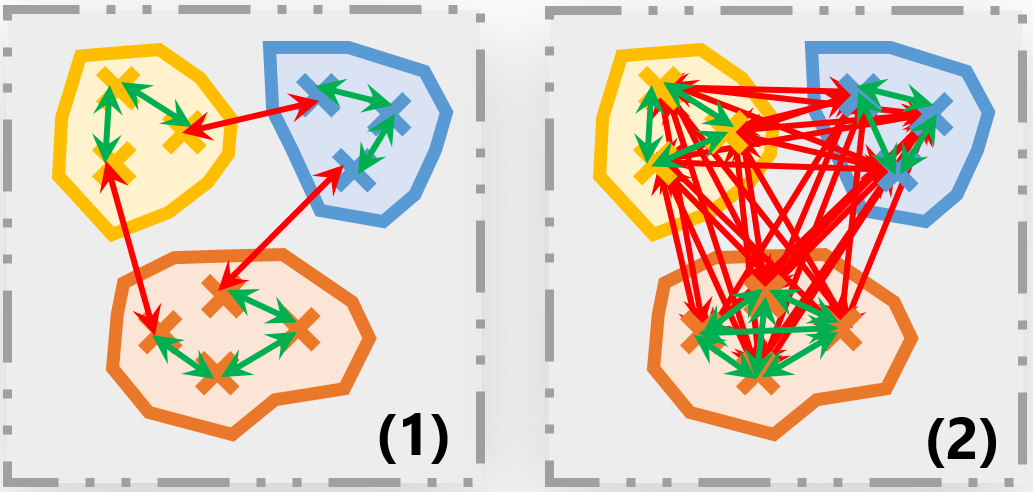
\includegraphics[width=0.5\textwidth]{figures/etude-nombre-contraintes-2-bornes-limites}
					\caption{
						Exemple de caractérisation exhaustive d'un jeu de données ($10$ données, $3$ classes) en ajoutant un nombre minimal de contraintes (cf. \textbf{(1)}) ou en ajoutant toutes les contraintes possibles (cf. \textbf{(2)}).
					}
					\label{figure:4.3.3-ETUDE-COUT-NOMBRE-CONTRAINTES-EXEMPLES}
				\end{figure}
			\end{leftBarAuthorOpinion}

		%%% Discussion.
		\subsubsection{Discussion}
		
			% Rappel de l'objectif.
			L'objectif de cette étude était de déterminer le nombre moyen de contraintes à devoir annoter pour modéliser un jeu de données avec un accord $90$\% de \texttt{v-measure} avec la vérité terrain utilisée.
			Cette estimation, dépendant de la taille du jeu de données manipulé, est représentée par l'\textsc{Equation~\ref{equation:4.3.3-ETUDE-COUT-NOMBRE-CONTRAINTES}}.
			\\
			
			% Discussion générale sur la pente.
			On peut constater que la relation entre la taille du jeu de données et le nombre de contraintes à annoter est linéaire (pente de $3.15$) : doubler la taille d'un jeu de données doublera donc la charge de travail incombant à l'expert métier.
			À première vue, une telle estimation représente une lourde charge d'annotation : \textbf{pour un jeu de $5~000$ données, il faut caractériser $15~750$ contraintes, ce qui correspond environ à $34$ heures d'annotation} d'après l'\textsc{Equation~\ref{equation:4.3.1-ETUDE-COUT-COUTS-TEMPS-ANNOTATION}} !
			Néanmoins, comme le nombre de contraintes possibles évolue en $ \mathcal{O}(\texttt{dataset\_size}) $, cette estimation aurait pu être bien pire et représenter $12~497~500$ contraintes (cf. \textsc{Figure~\ref{figure:4.3.3-ETUDE-COUT-NOMBRE-CONTRAINTES-EXEMPLES}} dans notre précédente précédente).
			Mieux encore, le nombre théorique minimal moyen de contraintes à annoter pour $5~000$ données n'est que $2.55$ fois plus faible que notre estimation ($6~175$ vs $15~750$, cf. notre précédente précédente), alors que cette borne minimale nécessite un échantillonnage "\textit{parfait}" permettant d'identifier le chemin minimal parcourant les clusters.
			Nous pouvons donc relativiser l'estimation faite avec l'\textsc{Equation~\ref{equation:4.3.3-ETUDE-COUT-NOMBRE-CONTRAINTES}} et en conclure que notre méthode un nombre de contraintes raisonnable à annoter.
			
			% Influence du jeu de données.
			Bien évidemment, une telle estimation est sensible au jeu de données utilisé comme référence (cf. \textsc{Figure~\ref{figure:4.3.3-ETUDE-COUT-NOMBRE-CONTRAINTES}}).
			Ici, la différence de pente mesurée est de $0.25$ (\texttt{p-valeur}: $> 0.999$), soit un écart moyen d'environ $8$\% par rapport à la modélisation moyenne.
			Toutefois, comme l'impact semble limité, nous maintenons la modélisation moyenne représentée par l'\textsc{Equation~\ref{equation:4.3.3-ETUDE-COUT-NOMBRE-CONTRAINTES}} pour la suite de nos estimations de coûts.
		
			% Note de l'auteur.
			\begin{leftBarAuthorOpinion}
				Il n'y a pas davantage de matière à discussion pour cette étude, car le principal résultat (l'\textsc{Equation~\ref{equation:4.3.3-ETUDE-COUT-NOMBRE-CONTRAINTES}}) est un résultat temporaire nécessaire à l'estimation du coût global d'un projet utilisant une méthodologie de \textit{clustering} interactif.
			\end{leftBarAuthorOpinion}
	
	%%%
	%%% Subsection 4.3.4: Estimation du temps total d'un projet d'annotation en combinant les précédentes études de coûts
	%%%
	\subsection{Estimation du temps total d'un projet d'annotation en combinant les précédentes études de coûts}
	\label{section:4.3.4-ETUDE-COUTS-TOTAL}
	
		% Equation finale.
		Résumons l'ensemble des modélisations réalisées lors des précédentes études (cf. sections \ref{section:4.3.1-ETUDE-COUTS-TEMPS-ANNOTATION}, \ref{section:4.3.2-ETUDE-COUTS-TEMPS-CALCUL} et \ref{section:4.3.3-ETUDE-COUT-NOMBRE-CONTRAINTES}) afin d'estimer le coût total d'un projet d'annotation employant une méthodologie basée sur le \textit{clustering} interactif et utilisant notre \textbf{paramétrage favori}\footnote{
			Paramétrage favori (atteindre $90$\% de \texttt{v-measure} avec un coût minimal).
		}.
		Dans les notations, $\texttt{dataset\_size}$ représente la taille du jeu de données à modéliser, et $\texttt{batch\_size}$ représente le nombre de contraintes que l'expert annote à chaque itération.

		%%% Résultats.
		\subsubsection{Synthèse des résultats}
			
			% Equation: Temps pour une itération (séquentielle).
			Tout d'abord, nous pouvons estimer le \textbf{temps moyen d'une itération de la méthode}, comprenant d'une part les temps d'exécution des algorithmes (\textit{prétraitement}, \textit{vectorisation}, \textit{clustering}, \textit{échantillonnage}) et d'autre part le temps d'annotation d'un lot de contraintes, grâce aux équations suivantes :
			\begin{equation}
				\label{equation:4.3.4-ETUDE-COUT-UNE-ITERATION-SEQUENTIELLE}
				\begin{cases}
					% Computation time.
					\texttt{computation\_time}~[s]&
						~\propto~0.17 \cdot \texttt{dataset\_size}\\
					% Annotation time.
					\texttt{annotation\_time}~[s]&
						~\propto~7.8 \cdot \texttt{batch\_size} \\
					% One iteration time (sequential).
					\texttt{iteration\_time(sequential)}~[s]&
						~\propto~\texttt{computation\_time} + \texttt{annotation\_time} \\
				\end{cases}
			\end{equation}
			
			% Equation: Nombre d'itérations (séquentielle).
			Ensuite, nous sommes en mesure d'anticiper le \textbf{nombre moyen de contraintes à annoter} pour modéliser le jeu de données avec un seuil de $90$\% de \texttt{v-measure}, et donc de déduire le nombre d'itérations nécessaire de la méthode, grâce aux équations suivantes :
			\begin{equation}
				\label{equation:4.3.4-ETUDE-COUT-NOMBRE-ITERATIONS-SEQUENTIEL}
				\begin{cases}
					% Constraints number.
					\texttt{constraints\_needed}~[\#] &
						~\propto~3.15 \cdot \texttt{dataset\_size} \\
					% Iterations number.
					\texttt{iterations\_needed}~[\#] &
						~\propto~\frac{\texttt{nb\_constraints}}{\texttt{batch\_size}} \\
				\end{cases}
			\end{equation}
			
			% Equation: Temps total pour un projet (séquentielle).
			Enfin, il suffit de combiner \textsc{Equation~\ref{equation:4.3.4-ETUDE-COUT-UNE-ITERATION-SEQUENTIELLE}} et \textsc{Equation~\ref{equation:4.3.4-ETUDE-COUT-NOMBRE-ITERATIONS-SEQUENTIEL}} pour estimer le temps total nécessaire à un projet d'annotation utilisant le \textit{clustering} interactif (c'est-à-dire en enchaînant successivement des étapes d'échantillonnage, d'annotation et de \textit{clustering}, cf. \textsc{Figure~\ref{figure:4.3.4-ETUDE-COUT-TOTAL-ARCHITECTURE}} (1)) pour converger vers $90$\% de \texttt{v-measure} :
			\begin{equation}
				\label{equation:4.3.4-ETUDE-COUT-TOTAL-SEQUENTIEL}
				\begin{cases}
					% Total time (sequential).
					\texttt{total\_time(sequential)}~[s] &
						~\propto~\texttt{iteration\_time} \cdot \texttt{iterations\_needed}
				\end{cases}
			\end{equation}
			
			% Figure.
			Ces estimations globales sont représentées sur la \textsc{Figure~\ref{figure:4.3.4-ETUDE-COUT-TOTAL}} en fonction de plusieurs taille de jeu de données et plusieurs tailles de lots d'annotation.

		%%% Discussion finale.
		\subsubsection{Discussion du coût total}
		
			% Rappel des objectifs.
			L'objectif de cette section consistait à déterminer les coûts relatifs à la tâche d'annotation de contraintes par un expert métier et au temps d'exécution des algorithmes intervenant dans notre implémentation du \textit{clustering} interactif.
			Pour cela, nous avons chronométré des annotateurs en situation réelle (cf. \textsc{Section~\ref{section:4.3.1-ETUDE-COUTS-TEMPS-ANNOTATION}}), estimé le temps de calcul de chaque algorithme implémenté (cf. \textsc{Section~\ref{section:4.3.2-ETUDE-COUTS-TEMPS-CALCUL}}) et trouvé le moyen de prédire le nombre de contraintes à annoter sur un jeu de données (cf. \textsc{Section~\ref{section:4.3.3-ETUDE-COUT-NOMBRE-CONTRAINTES}}).
			Nous avons pu montré qu'une annotation de contraintes est plus rapide qu'une annotation par label et nous conseillons, d'après notre analyse empirique, des sessions d'annotation de moins de $150$ contraintes pour ne pas épuiser l'annotateur.
			Sur le paramétrage de la méthode, nous avons rejeté l'usage d'algorithmes de \textit{clustering} de type hiérarchiques à cause de leur lenteur, au profit du KMeans (\texttt{clust.kmeans.cop}).
			Notre paramétrage favori, permettant d'atteindre $90$\% de \texttt{v-measure} avec un coût minimal, est ainsi constitué d'un prétraitement simple (\texttt{prep.simple}), d'une vectorisation TF-IDF (\texttt{vect.tfidf}), d'un \textit{clustering} KMeans avec modèle COP (\texttt{clust.kmeans.cop}) et d'un échantillonnage des données les plus proches dans des clusters différents (\texttt{sampl.closest.diff}).
			Enfin, pour atteindre cet objectif de \texttt{v-measure}, le nombre moyen de contraintes à annoter avec notre méthodologie semble rester linéairement proportionnel à la taille du jeu de données à modéliser, ce qui est encourageant au regard de la combinatoire de contraintes possibles.
			\\
			
			% Annonce des résultats : c'est long !
			La mise en commun de ces résultats se retrouvent dans \textsc{Equation~\ref{equation:4.3.4-ETUDE-COUT-UNE-ITERATION-SEQUENTIELLE}}, \textsc{Equation~\ref{equation:4.3.4-ETUDE-COUT-NOMBRE-ITERATIONS-SEQUENTIEL}} et \textsc{Equation~\ref{equation:4.3.4-ETUDE-COUT-TOTAL-SEQUENTIEL}}.
			Comme le nombre de données à annoter est inversement proportionnel au nombre d'itération à réaliser, nous avons le dilemme suivant : soit nous annotons de petits lots ($50$ contraintes) pour rapidement intégrer les contraintes et permettre à l'annotateur de se reposer régulièrement, mais ce dernier va en contrepartie devoir attendre plus souvent la fin des exécutions du \textit{clustering} ; soit nous annotons des lots plus conséquents ($150$ contraintes) pour diminuer le nombre d'itérations et exécuter moins de \textit{clustering}, mais cela risque d'épuiser l'opérateur avec des grosses charges d'annotation.
			Dans les deux cas, \textbf{le coût total semble élevé} : pour un jeu de $5~000$ points de données, et avec des tailles d'échantillons compris entre $50$ et $150$ contraintes, il faut entre $59$ et $110$ heures de travail (\textit{$34$ heures d'annotations et entre $25$ et $76$ heures d'attente de la fin d'exécution d'algorithmes suivant la taille des lots}).
			En considérant une journée de travail de $7$ heures, cela représente une charge contenue entre $8.4$ et $15.7$ jours pour avoir un jeu de donnée fiable à $90$\% de \texttt{v-measure}.
			Pour finir, nous ajoutons $1$ jour pour combler l'écart théorique de $10$\% de \texttt{v-measure} en corrigeant manuellement le résultat obtenu, et $1$ jour supplémentaire pour interpréter et nommer chaque \textit{cluster} (voir. \textsc{Algorithme~\ref{algorithm:3.2-CLUSTERING-INTERACTIF}}, \textit{ligne 13}).
			Au final, pour un ensemble de $5~000$ données, il faut donc entre $8.4$ {\footnotesize $(+2)$} et $15.7$ {\footnotesize $(+2)$} jours de travail à un expert métier pour obtenir une base d'apprentissage avec une méthodologie basée sur le \textit{clustering} interactif.
			
			% Critique du résultat : comparaison avec une annotation classique, avoir plusieurs annotateurs, ...
			Pour critiquer l'approximation que nous avons faite lors de cette section, nous essayons de la comparer le temps nécessaire qu'il aurait fallu à un projet d'annotation traditionnelle, comme décrit en \textsc{Section~\ref{section:2.2.1-ORGANISATION-ANNOTATION-ETAPES-CLES}} (cycle \texttt{MATTER}), et notre proposition de cycle d'annotation avec le \textit{clustering} interactif, visible en \textsc{Figure~\ref{figure:4.3.4-ETUDE-COUT-TOTAL-ARCHITECTURE}} (1).
			En nous basant sur un ensemble de $5~000$ données à annoter, nous estimons qu'il faut :
			$1$ jour de travail pour définir une représentation des données en modèle de classification ;
			$4$ jours de travail pour annoter $5~000$ données (à raison de $20$ secondes par données, estimation haute inspirée de \cite{pradhan-etal:2007:semeval2007-task-17} où la "\textit{désambiguïsation du sens des mots}", présentée comme une tâche de classification, demande $17.5$ secondes par données) ;
			$2$ jours de marge d'erreur pour changer de modèle de représentation s'il ne semble pas adapté aux données en cours d'annotation.
			Au total, nous estimons donc qu'il faut $5$ {\footnotesize $(+2)$} jours de travail à un expert métier pour obtenir une base d'apprentissage avec une méthodologie traditionnelle.
			\textbf{En l'état, nous pouvons donc conclure que le \textit{clustering} interactif que nous proposons est en moyenne deux fois plus coûteux qu'une annotation manuelle classique ($8.4$ {\footnotesize $(+2)$} à $15.7$ {\footnotesize $(+2)$} jours vs $5$ {\footnotesize $(+2)$} jours), ce qui peut être un frein à son utilisation en situation réelle}.
			
			% Pistes d'amélioration : Augmenter la taille des lots d'annotation + Augmenter le nombre d'annotateurs + paralléliser annotation et clustering, ...
			Afin d'accélérer la phase d'annotation et de diminuer le nombre d'itérations, il est bien entendu possible d'augmenter la taille des échantillons de contraintes à annoter ou d'ajouter plusieurs opérateurs.
			Cependant, une telle solution ne permet toujours pas d'être compétitif avec l'annotation traditionnelle si cette dernière dispose aussi de plusieurs opérateurs (\textit{avec $2$ annotateurs : de $6.5$ {\footnotesize $(+2)$} à $13.3$ {\footnotesize $(+2)$} jours vs $3$ {\footnotesize $(+2)$} jours ; avec $4$ annotateurs : de $4.8$ {\footnotesize $(+2)$} à $12.1$ {\footnotesize $(+2)$} jours vs $2$ {\footnotesize $(+2)$} jours}).
			Une autre piste, plus prometteuse, consiste plutôt à adapter notre méthode pour exploiter les temps d'attente lors de l'exécution d'un \textit{clustering}.
			

		%%% Ouverture
		\subsection{Ouverture vers une annotation en parallèle du \textit{clustering}}
		
			% Idée : Optimiser le temps d'attente.
			Notre méthodologie d'annotation basée sur le \textit{clustering} interactif est pénalisée par la séquentialité des actions à réaliser.
			En effet, l'annotateur doit attendre la fin d'un de l'exécution des algorithmes de \textit{clustering} et d'échantillonnage avant de pouvoir travailler.
			D'après nos précédentes estimations sur un jeu de $5~000$ données, l'opérateur doit attendre entre $25$ et $76$ heures en fonction de la taille de lots d'annotation choisie, et une idée à explorer consiste à optimiser ce temps d'attente.
			
			% Réalisation : Paralléliser annotation et \textit{clustering} !
			L'amélioration envisagée consiste à \textbf{réaliser l'annotation de contraintes en parallèle de l'exécution du \textit{clustering}}, comme représenté dans la \textsc{Figure~\ref{figure:4.3.4-ETUDE-COUT-TOTAL-ARCHITECTURE}} (2).
			Dans cette version, l'échantillonnage se base toujours sur le résultat du \textit{clustering} de l'itération précédente, mais le \textit{clustering} intègre les contraintes annotées avec un décalage d'une itération.
			Un tel changement permet de limiter le temps d'attente de l'opérateur et d'optimiser l'enchaînement des algorithmes.

			% Figure architecture.
			\begin{figure}[!htb]
				\centering
				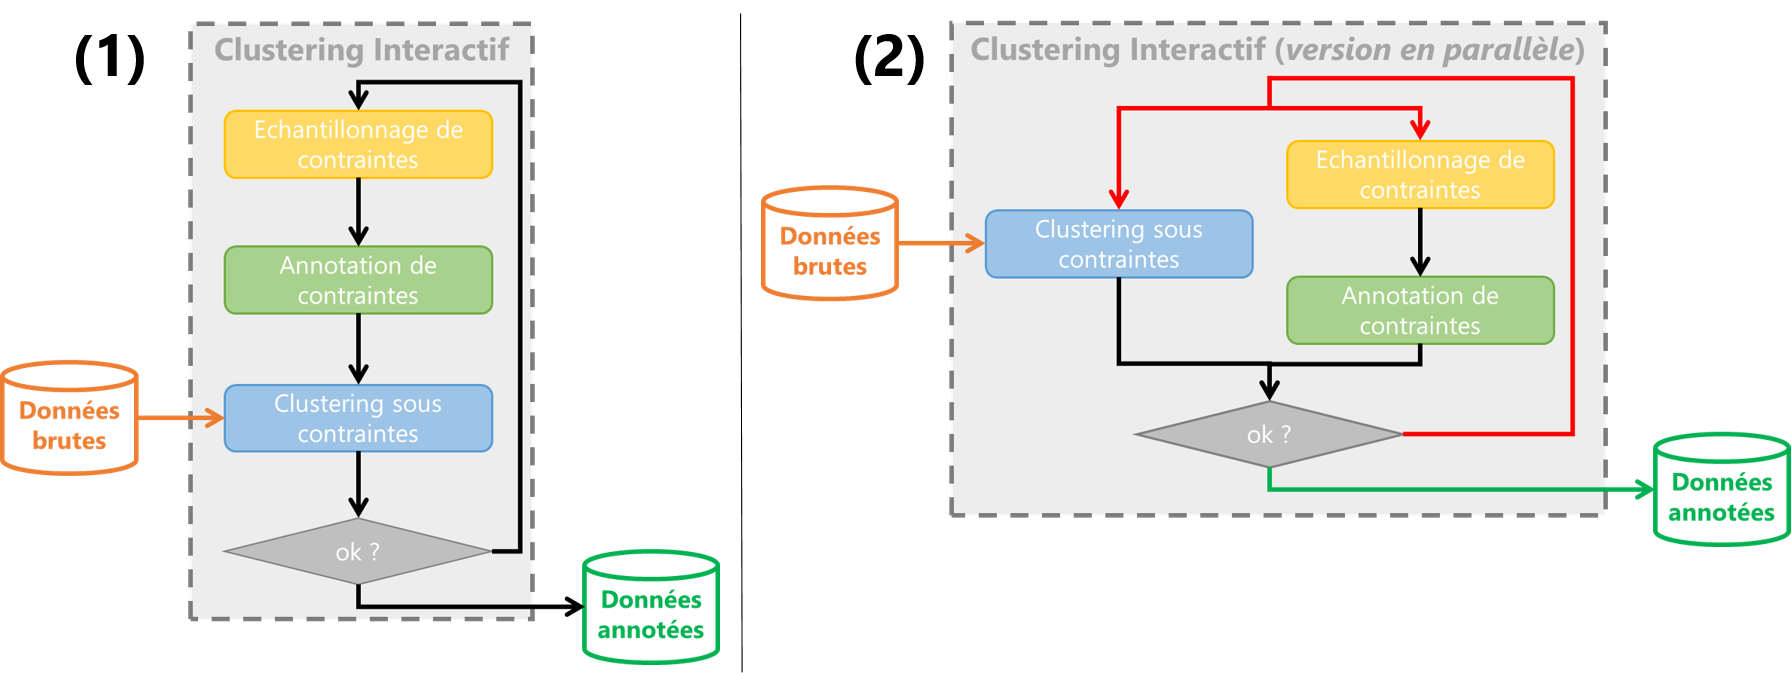
\includegraphics[width=0.95\textwidth]{figures/interactive-clustering-architecture-sequentielle-vs-parallele}
				\caption{
					Schéma comparatif des architectures du \textit{clustering} interactif : \textbf{(1)} représente la version séquentielle initialement présentée en \textsc{Chapitre~\ref{chapter:3-CLUSTERING-INTERACTIF}} où le \textit{clustering} s'adapte avec les annotation de l'itération en cours ; \textbf{(2)} représente l'évolution en mode \textit{parallèle} où le \textit{clustering} s'adapte avec les annotations de l'itération précédente (décalage d'une itération).
				}
				\label{figure:4.3.4-ETUDE-COUT-TOTAL-ARCHITECTURE}
			\end{figure}
			
			% Equation : Adaptation du Temps pour une itération (parallèle).
			Avec cette version, le temps nécessaire à une itération correspond à la durée la plus longue entre le temps d'annotation et le temps de calcul des algorithmes.
			Nous pouvons donc adapter l'\textsc{Equation~\ref{equation:4.3.4-ETUDE-COUT-UNE-ITERATION-SEQUENTIELLE}} par l'équation suivante :
			\begin{equation}
				\label{equation:4.3.4-ETUDE-COUT-UNE-ITERATION-PARALLELE}
				\begin{cases}
					% Computation time.
					\texttt{computation\_time}~[s]&
						~\propto~0.17 \cdot \texttt{dataset\_size}\\
					% Annotation time.
					\texttt{annotation\_time}~[s]&
						~\propto~7.8 \cdot \texttt{batch\_size} \\
					% One iteration time (parallel).
					\texttt{iteration\_time(parallel)}~[s]&
						~\propto~max(\texttt{computation\_time}, \texttt{annotation\_time}) \\
				\end{cases}
			\end{equation}
			
			% Equation : Adaptation du Nombre d'itérations (parallèle).
			Ensuite, afin de limiter les pertes de temps (humain et machine), nous pouvons choisir une taille de lot d'annotation rendre les deux durées équivalentes.
			Nous déduisons donc les changements suivants dans l'\textsc{Equation~\ref{equation:4.3.4-ETUDE-COUT-NOMBRE-ITERATIONS-SEQUENTIEL}} :
			\begin{equation}
				\label{equation:4.3.4-ETUDE-COUT-NOMBRE-ITERATIONS-PARALLELE}
				\begin{cases}
					% Batch size.
					\texttt{optimal\_batch\_size}~[\#]&
						~\propto~\frac{\texttt{computation\_time}}{7.8}
						~\propto~0.0218 \cdot \texttt{dataset\_size} \\
					% Iterations number.
					\texttt{iterations\_needed}~[\#] &
						~\propto~\frac{\texttt{nb\_constraints}}{\texttt{optimal\_batch\_size}}
						~\propto~144.5 \\
				\end{cases}
			\end{equation}
			
			% Equation: Adaptation du Temps total pour un projet (parallèle).
			Enfin, il suffit de combiner \textsc{Equation~\ref{equation:4.3.4-ETUDE-COUT-UNE-ITERATION-PARALLELE}} et \textsc{Equation~\ref{equation:4.3.4-ETUDE-COUT-NOMBRE-ITERATIONS-PARALLELE}} pour estimer le temps total nécessaire à un projet d'annotation pour converger vers $90$\% de \texttt{v-measure} utilisant la version parallèle du \textit{clustering} interactif :
			\begin{equation}
				\label{equation:4.3.4-ETUDE-COUT-TOTAL-PARALLELE}
				\begin{cases}
					% Total time (parallel).
					\texttt{total\_time(parallel)}~[s] &
						~\propto~\texttt{iteration\_time} \cdot \texttt{iterations\_needed} \\
					\texttt{total\_time(parallel)}~[s] &
						~\propto~24.6 \cdot \texttt{dataset\_size}
				\end{cases}
			\end{equation}
			
			% Figure.
			Ces estimations mises à jour sont représentées sur la \textsc{Figure~\ref{figure:4.3.4-ETUDE-COUT-TOTAL}} en fonction de plusieurs taille de jeu de données, et permettent de faire la comparaison avec la version séquentielle initialement présentée.
			
			% Figures.
			%
			\begin{figure}[!htb]
				\centering
				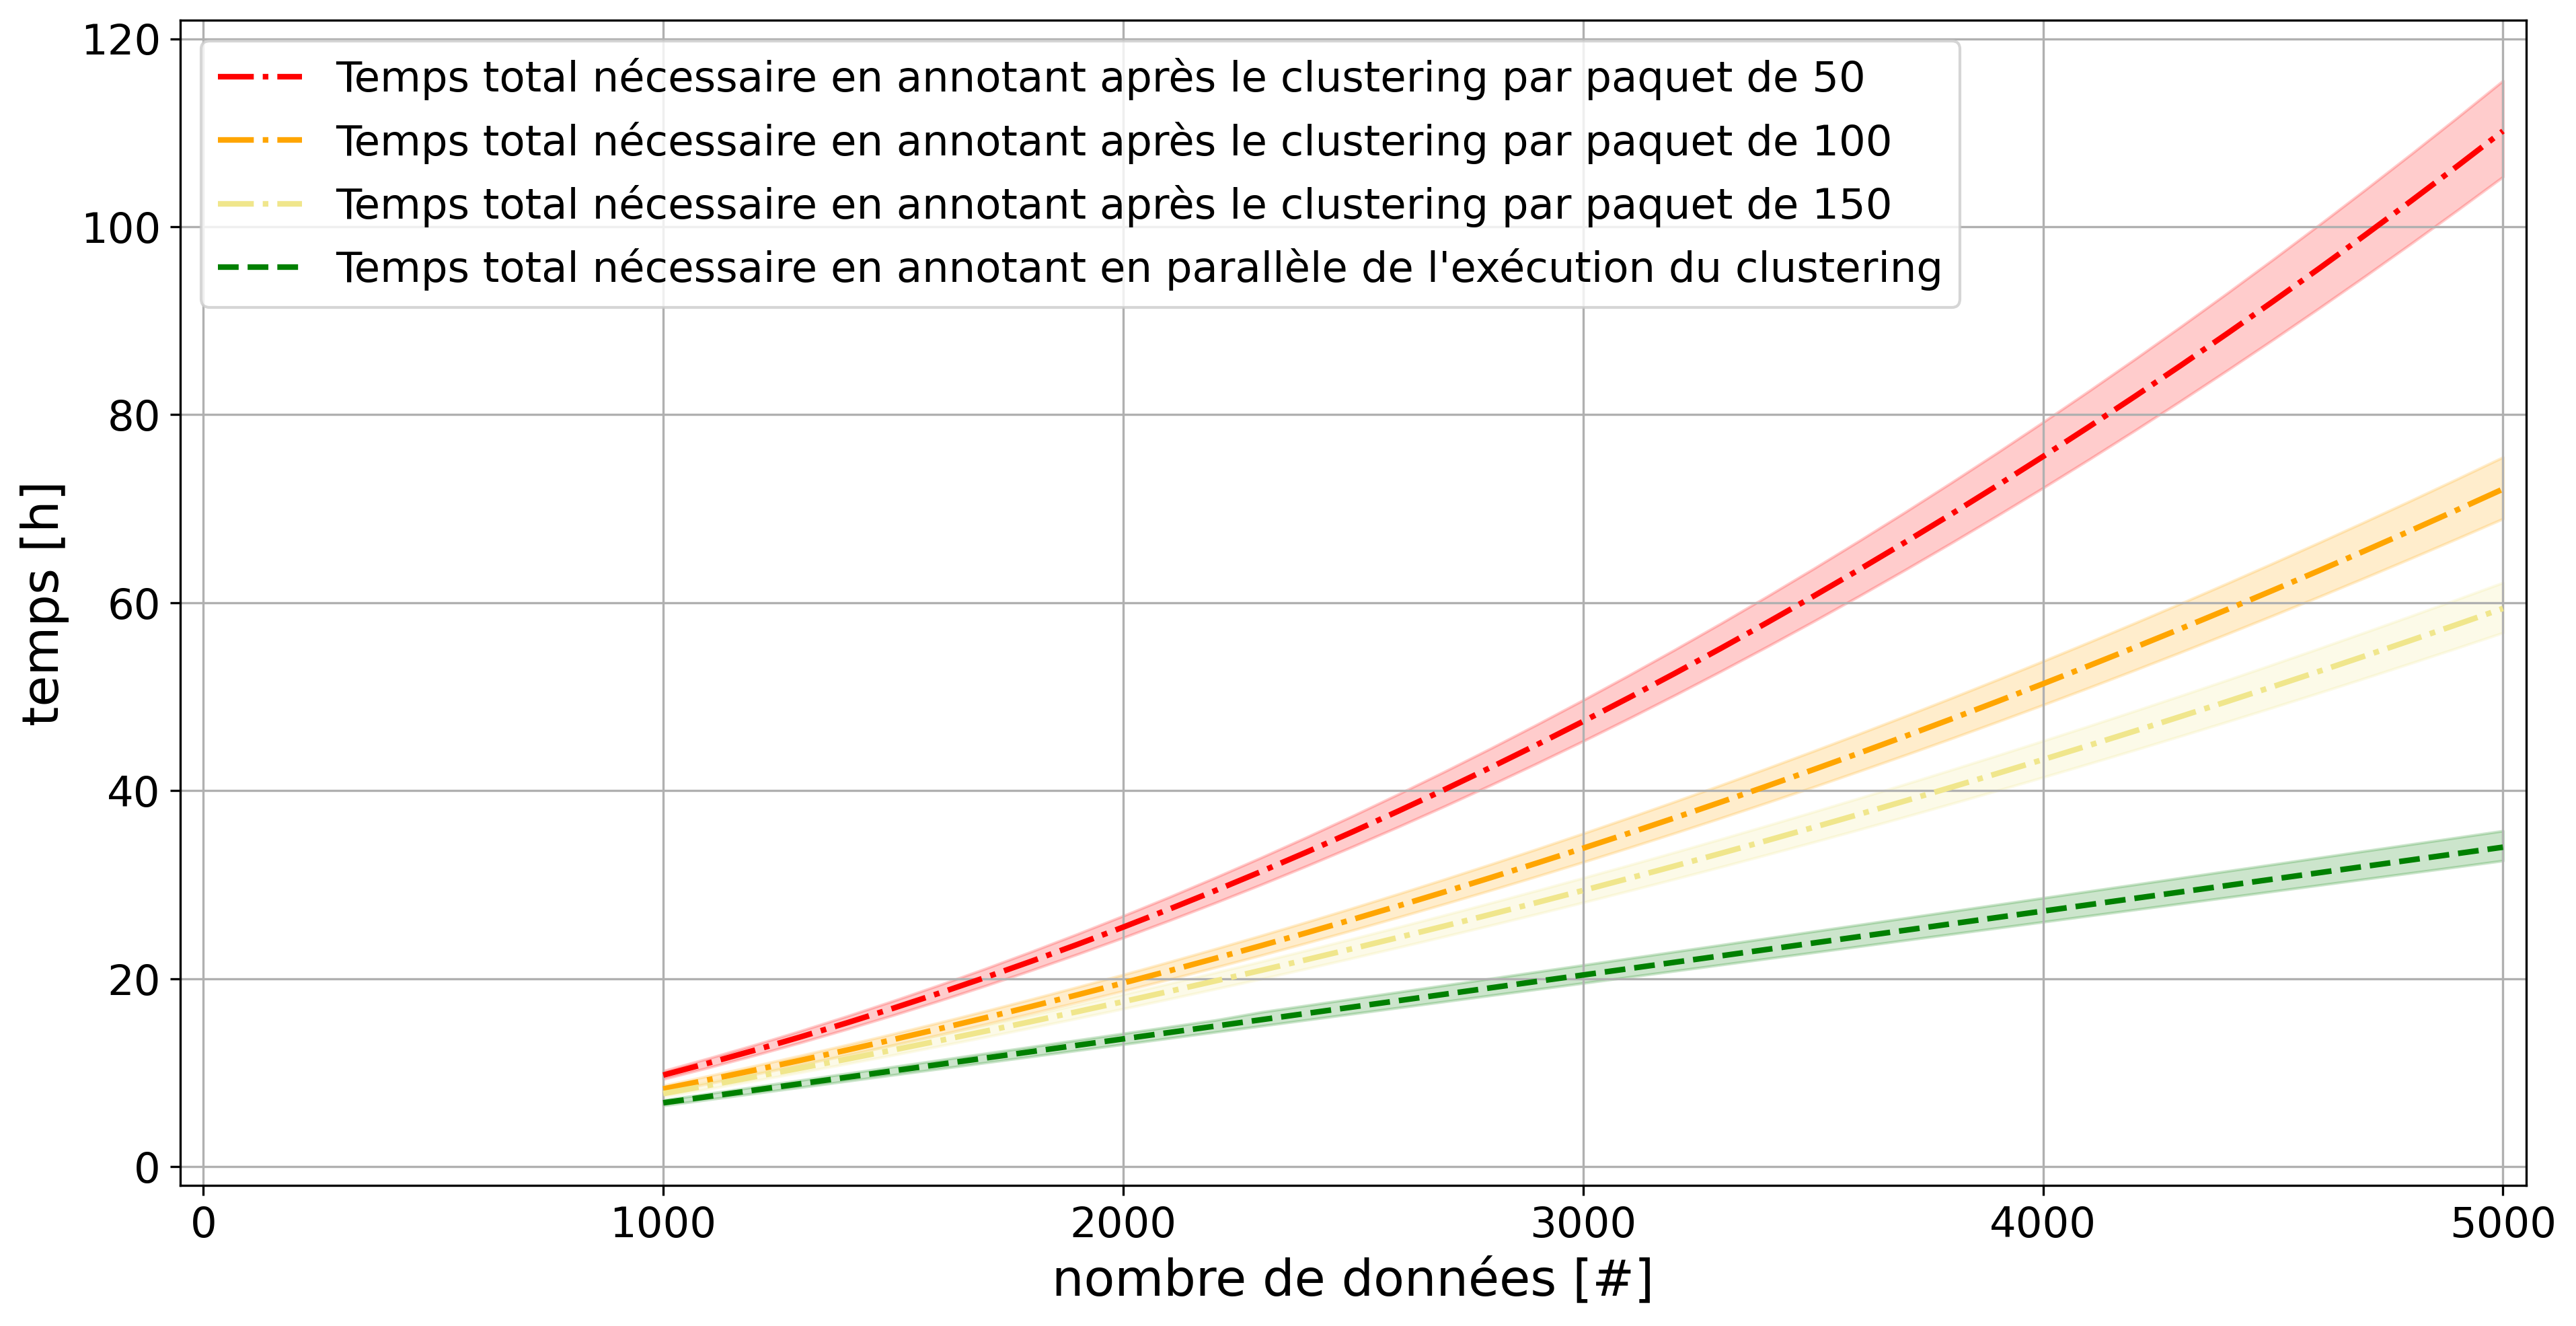
\includegraphics[width=0.95\textwidth]{figures/etude-temps-total-2-modelisation-parallele}
				\caption{
					Estimation du temps total nécessaire (en heures) pour modéliser un jeu de données avec notre \textbf{paramétrage favori} du \textit{clustering} interactif afin d'obtenir une annotation partielle (\textit{atteindre une \texttt{v-measure} de $90$\%}), en fonction de plusieurs taille de jeu de données, plusieurs tailles de lots d'annotation, et mettant en opposition l'approche séquentielle (\textit{annotation puis le clustering}) et l'approche parallèle (\textit{annotation pendant le clustering}).
				}
				\label{figure:4.3.4-ETUDE-COUT-TOTAL}
			\end{figure}
			
			% Résultats et discussion : linéaire, 25 x dataset size : c'est acceptable !
			Nous pouvons déjà remarquer que le coût d'annotation du projet devient linéaire en nombre de données (pente de $24.6$ secondes) et nécessite un nombre fixe de $145$ itérations.
			En reprenant une base de $5~000$ données et une marge de $2$ jours pour corriger et nommer les \textit{clusters}\footnote{
				voir. \textsc{Algorithme~\ref{algorithm:3.2-CLUSTERING-INTERACTIF}}, \textit{ligne 13}.
			}, cela représente $4.8$ {\footnotesize $(+2)$} jours de travail, un estimation équivalente à une annotation traditionnelle qui nécessite $5 $ {\footnotesize $(+2)$} jours de travail d'après nos approximations.
			De plus, si nous ajoutons des plusieurs opérateurs, cette version parallèle reste compétitive (\textit{avec $2$ annotateurs : $2.5$ {\footnotesize $(+2)$} jours vs $3$ {\footnotesize $(+2)$} jours ; avec $4$ annotateurs : $1.3$ jours vs $2$ {\footnotesize $(+2)$} jours}).
			Cette découverte est très encourageante, car cela confirme qu'une méthodologie basée sur notre implémentation du \textit{clustering} interactif \textbf{permet d'obtenir une base d'apprentissage avec un coût temporel équivalent à un projet traditionnel} utilisant une annotation par label.
			Cette méthode est d'autant plus intéressante qu'elle fait intervenir un mécanisme d'annotation rapide et intuitif pour un expert métier.
			
			% Conclusion.
			\begin{leftBarSummary}
				Au cours de cette étude de coûts, nous avons pu déduire que :
				\begin{itemize}
					\item[\itemok] L'annotation d'une contrainte nécessite en moyenne $8$ secondes : cette tâche est rapide et intuitive (cf. \textsc{Section~\ref{section:4.3.1-ETUDE-COUTS-TEMPS-ANNOTATION}}) ;
					\item[\itemok] Notre paramétrage favori, permettant d'atteindre $90$\% de \texttt{v-measure} avec un coût minimal, est constitué du prétraitement simple (\texttt{prep.simple}), de la vectorisation TF-IDF (\texttt{vect.tfidf}), du \textit{clustering} KMeans avec modèle COP (\texttt{clust.kmeans.cop}) et de l'échantillonnage des données les plus proches dans des clusters différents (\texttt{sampl.closest.diff}). Ce paramétrage a un coût moyen de $0.17 \cdot \texttt{dataset\_size}$ secondes (cf. \textsc{Section~\ref{section:4.3.2-ETUDE-COUTS-TEMPS-CALCUL}}) ;
					\item[\itemok] Une adaptation optimale de notre méthodologie consiste à paralléliser l'exécution du \textit{clustering} et l'annotation de contraintes afin de limiter les temps d'attente inutiles. Une telle méthode a un coût moyen de $24.6 \cdot \texttt{dataset\_size}$ pour atteindre $90$\% de \texttt{v-measure}, auquel on ajoute $2$ jours de travail pour raffiner les clusters et les nommer. Ce temps est compétitif à une annotation traditionnelle (cf. \textsc{Section~\ref{section:4.3.4-ETUDE-COUTS-TOTAL}}) ;
					\item[\itemok] Cette étude met en avant l'intérêt des interactions homme-machine : (1) l'expert métier se recentre sur son domaine de compétence avec une caractérisation proche de ses connaissances ("\textit{les données sont-elles similaires ?}") et (2) la machine optimise l'intervention de l'expert pour que ce dernier soit toujours pertinent dans ses contributions.
				\end{itemize}
			\end{leftBarSummary}
		
		% Transition: Vers Pertinence et Rentabilité.
		Dans les sections suivantes, nous allons nous intéressé à l'analyse des résultats de cette méthode.
		En effet, en situation réelle, nous n'avons pas accès à la vérité terrain car elle est justement en cours de construction.
		Il nous est donc impossible d'estimer notre seuil de \texttt{v-measure}, et donc incapable de s'arrêter à $90$\% de \texttt{v-measure}.
		Nous nous intéressons donc à l'estimation de la valeur métier d'un résultat de \textit{clustering} (cf. hypothèse de pertinence en \textsc{Section~\ref{section:4.4-HYPOTHESE-PERTINENCE}}) et à la définition de cas d'arrêt agnostique d'une vérité terrain (cf. hypothèse de rentabilité en \textsc{Section~\ref{section:4.5-HYPOTHESE-RENTABILITE}}).
	
	
	%%%%%--------------------------------------------------------------------
	%%%%% Section 4.4: Hypothèse de pertinence.
	%%%%%--------------------------------------------------------------------
	\newpage
	\section{Évaluation de l'hypothèse de pertinence}
\label{section:4.4-HYPOTHESE-PERTINENCE}

	%%% Introduction / Transition.
	Jusqu'à présent, nous avons analysé la performance et l'évolution des résultats de notre implémentation du \textit{clustering} interactif à l'aide d'une vérité terrain (cf. calcul de \texttt{v-measure}).
	Cependant, une telle référence n'est pas accessible en situation réelle (l'objectif de notre méthode est précisément de la construire).
	Nous devons donc nous intéresser à d'autres moyens d'estimer la pertinence des bases d'apprentissages obtenus et de définir comment définir l'exploitabilité d'un résultat.
	Ainsi, nous aimerions vérifier l'hypothèse suivante :
	
	%%% Formulation des hypothèses:
	\begin{tcolorbox}[
		title=\faVial~\textbf{Hypothèse de pertinence}~\faVial,
		colback=colorTcolorboxHypothesis!15,
		colframe=colorTcolorboxHypothesis!75,
		width=\linewidth
	]
		« \textbf{
			Au cours d'une méthodologie d'annotation basée sur le \textit{clustering} interactif, il est possible à un expert métier d'évaluer rapidement la pertinence de la base d'apprentissage en construction sans utiliser de vérité terrain.
		} » \\
		
		% Figure.
		La \textsc{Figure~\ref{figure:4.4-HYPOTHESE-PERTINENCE}} illustre cette hypothèse et l'espoir de pouvoir caractériser la qualité de la base d'apprentissage en cours de construction en fonction d'une valeur métier exprimée par un expert.
		%
		\begin{figure}[H]  % keep [H] to be in the tcolorbox.
			\centering
			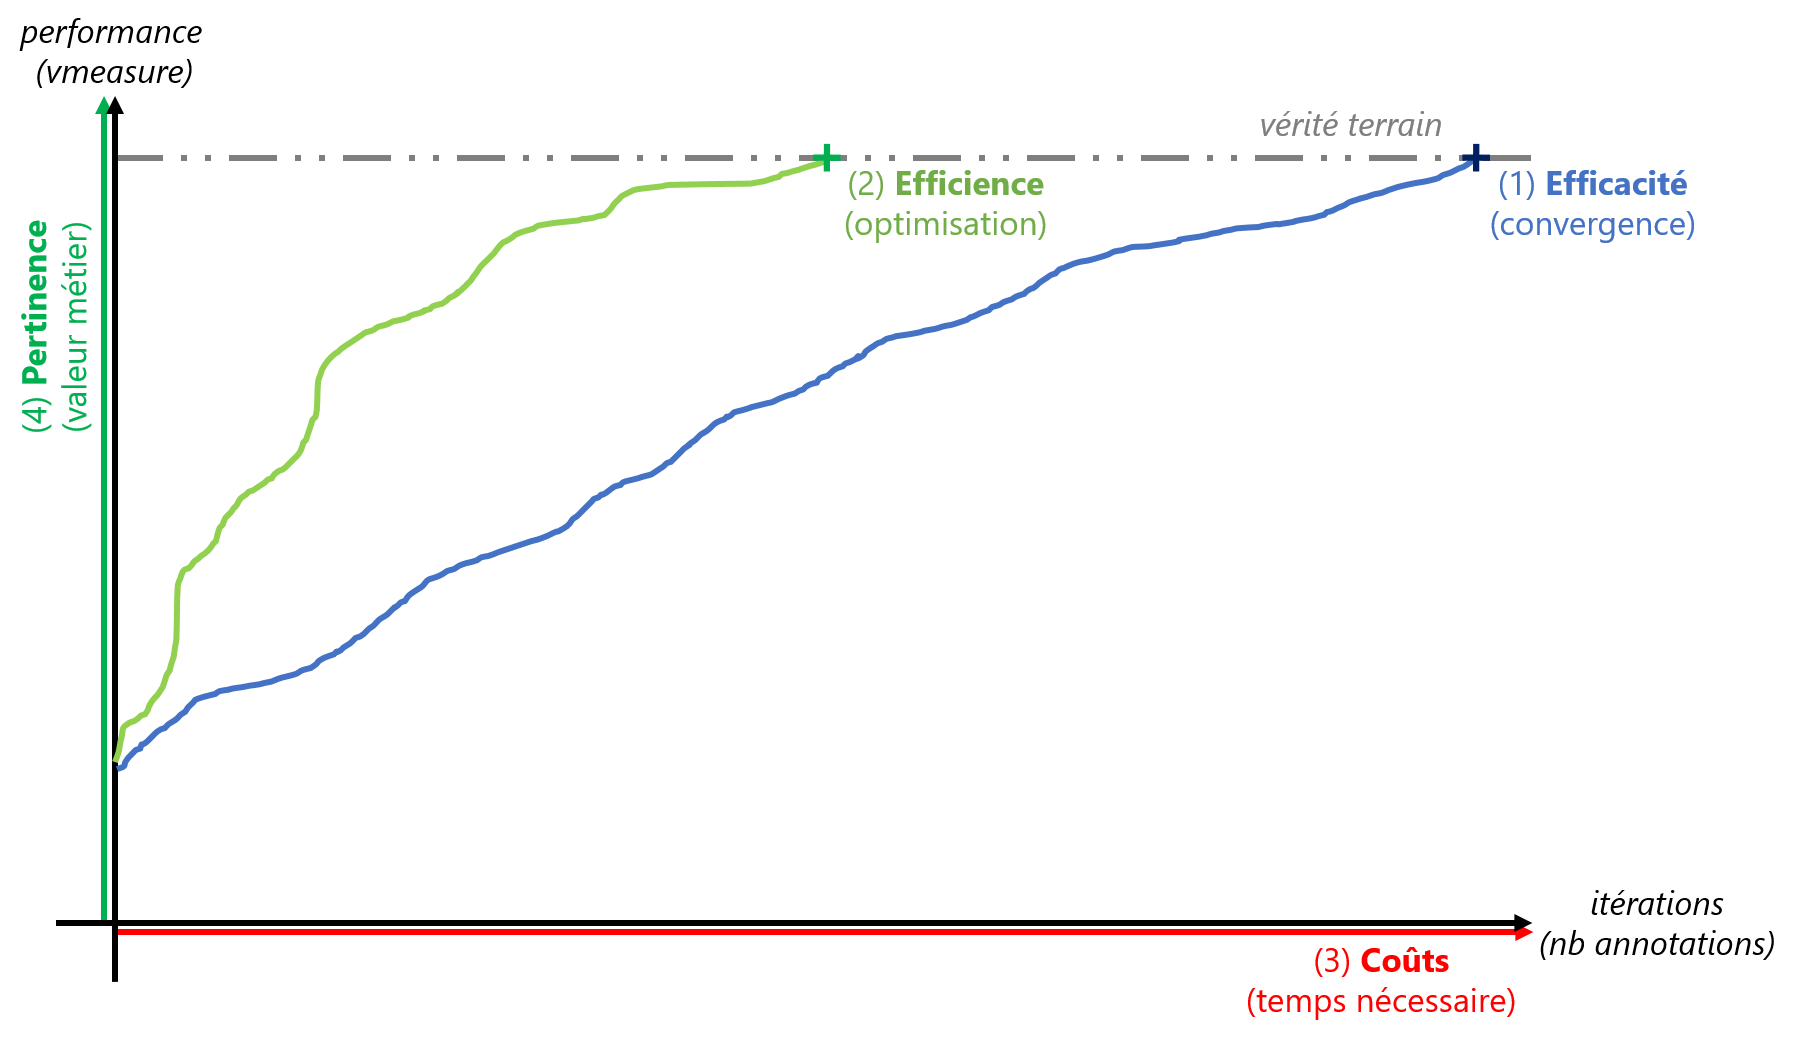
\includegraphics[width=0.95\textwidth]{figures/hypotheses-04-pertinence}
			\caption{Illustration des études réalisées sur le \textit{clustering} interactif (\textit{étape 4/6}) en schématisant l'évolution de la pertinence (\textit{valeur métier évaluée par l'expert et exprimé en nombre de clusters}) d'une base d'apprentissage en cours de construction en fonction du coût temporel de la méthode (\textit{temps nécessaire à l'expert métier et à la machine}).}
			\label{figure:4.4-HYPOTHESE-PERTINENCE}
		\end{figure}

	\end{tcolorbox}
		
	% Résumé de l'étude.
	Afin de vérifier cette hypothèse, nous explorons trois approches :
	\begin{itemize}
		\item une \textbf{vérification par un expert} du partitionnement des données obtenus, en parcourant manuellement le contenu des \textit{clusters} et en donnant un avis sur l'exploitabilité de ces derniers (cf. \textsc{Section~\ref{section:4.4.1-ETUDE-PERTINENCE-VERIFICATION-MANUELLE}}) ;
		\item une analyse des \textbf{patterns linguistiques saillants} dans la base d'apprentissage à l'aide d'une stratégie de sélection des composantes principales d'un modèle (cf. \textsc{Section~\ref{section:4.4.2-ETUDE-PERTINENCE-PATTERNS-LINGUISTIQUES}}),
		\item et une approche utilisant un \textbf{résumé automatique de thématique} par un modèle de langue, permettant de décrire succinctement le contenu des \textit{clusters} en une phrase. (cf. \textsc{Section~\ref{section:4.4.3-ETUDE-PERTINENCE-RESUME-AUTOMATIQUE}}).
	\end{itemize}
	
	
	%%%
	%%% Subsection 4.4.1: Étude d'une vérification manuelle de la valeur métier d'une base d'apprentissage par un expert
	%%%
	\subsection{Étude d'une vérification manuelle et non assistée de la valeur métier d'une base d'apprentissage par un expert}
	\label{section:4.4.1-ETUDE-PERTINENCE-VERIFICATION-MANUELLE}
		
		% Objectif de l'expérience.
		Afin d'estimer la pertinence d'un résultat de \textit{clustering}, notre première intuition consiste à demander simplement l'avis d'un expert sur la base d'apprentissage en cours de construction.
		En lui posant certaines questions, nous espérons obtenir une description qualitative de chaque \textit{cluster} et ainsi déduire quand le résultat du \textit{clustering} interactif devient exploitable pour définir et entraîner un modèle de classification.
	
		%%% Protocole expérimental.
		\subsubsection{Protocole expérimental}
			
			% Pseudo-code.
			Pour résumer le protocole expérimental que nous décrivons ci-dessous, vous pouvez vous référer au pseudo-code décrit dans \textsc{Algorithme~\ref{algorithm:4.4.1-ETUDE-PERTINENCE-VERIFICATION-MANUELLE-PROTOCOLE}]}.
			%
			\begin{algorithm}[!htb]
				\begin{algorithmic}[1]
					\Require jeux de données annotés (vérité terrain) de tailles différentes
					\State \textbf{initialisation (données)}: récupérer ou générer les données et la vérité terrain
					\State \textbf{initialisation (contraintes)}: créer une liste vide de contraintes
					\State \textbf{prétraitement}: supprimer le bruit dans les données avec \texttt{prep.simple}
					\State \textbf{vectorisation}: transformer les données en vecteurs avec \texttt{vect.tfidf}
					\State \textbf{clustering initial}: regrouper les données par similarité avec \texttt{clust.kmeans.cop}
					\State \textbf{évaluation manuelle}: juger de l'exploitabilité de chaque \textit{cluster}
					\Repeat
						\State \textbf{échantillonnage}: sélectionner de nouvelles contraintes à annoter
						\State \textbf{simulation d'annotation}: ajouter des contraintes avec \texttt{samp.closest.diff}
						\State \textbf{clustering}: regrouper les données par similarité avec \texttt{clust.kmeans.cop}
						\State \textbf{évaluation manuelle}: juger de l'exploitabilité de chaque \textit{cluster}
						\State \textbf{labellisation manuelle}: nommer chaque \textit{cluster} exploitable
					\Until{annotation de toutes les contraintes possibles}
					\State \textbf{analyse}: afficher l'évolution de l'exploitabilité de chaque itération de \textit{clustering}
					\Ensure discussion sur la complexité de la tâche et sur l'évolution de l'exploitabilité
				\end{algorithmic}
				\caption{Description en pseudo-code du protocole expérimental de l'étude de vérification manuelle non assistée de la valeur métier d'une base d'apprentissage.}
				\label{algorithm:4.4.1-ETUDE-PERTINENCE-VERIFICATION-MANUELLE-PROTOCOLE}
			\end{algorithm}
			
			% Description de la vérité terrain.
			Nous utilisons comme vérité terrain le jeu de données \texttt{Bank Cards (v1.0.0)} : ce dernier traite des demandes les plus fréquentes des clients en ce qui concerne la gestion de leur carte bancaire.
			Il est composé de $500$ questions rédigées en français et réparties en $10$ classes (\texttt{perte ou vol de carte}, \texttt{carte avalée}, \texttt{commande de carte}, ...).
			Pour plus de détails, consultez l'annexe~\ref{annex:C.1-DATASET-BANK-CARDS}.
			
			% Description des tentatives de la méthode.
			Sur ce jeu de données, nous exécutons une tentative complète
			\footnote{Tentative complète : itérations d'échantillonnage, d'annotation et de \textit{clustering} jusqu'à annotation de toutes les contraintes possibles.}
			de la méthode du \textit{clustering} interactif utilisant notre paramétrage favori, et cette tentative est répétée $5$ fois pour contrer les aléas statistiques des exécutions.
			
			% Description de l'évaluation manuelle.
			Au cours des itérations, un expert qualifie chaque \textit{cluster} en donnant son avis sur sa valeur métier.
			Afin d'encadrer ses réponses, nous lui demandons d'analyser trois aspects :
			\begin{itemize}
				\item est-ce que le \textit{cluster} a une thématique principale \textbf{bien définie} ? (\textit{en effet, comment interpréter un cluster sans définition claire ?})
				\item est-ce que le \textit{cluster} est constitué par un nombre suffisant de données ? (\textit{en effet, comment entraîner un modèle de classification sans données ?})
				\item est-ce que le \textit{cluster} n'est pas trop bruité ? (\textit{en effet, comment avoir de bonnes performances si la base d'apprentissage n'est pas fiable ?})
			\end{itemize}
			
			L'avis exprimé par l'expert métier est alors classé en trois niveaux :
			\begin{itemize}
				\item \textbf{exploitable} : le \textit{cluster} possède (1) une thématique bien définie, (2) un nombre de données suffisant pour entraîner un modèle de classification et (3) peu de bruit ; ce \textit{cluster} peut donc être exploité en l'état ou avec peu de modifications manuelles ;
				\item \textbf{partiellement exploitable} : soit le \textit{cluster} est composé de plusieurs de thématiques (\textit{deux ou trois}), soit il ne comporte pas pas assez de données (\textit{moins d'une vingtaines}), soit il est bruité (\textit{au moins un quart de bruit}) ; ce \textit{cluster} donne une première base pour créer une classe, mais un travail manuel est nécessaire (\textit{ajout de données, tri du bruit, ...}) ;
				\item \textbf{non exploitable} : soit le \textit{cluster} ne contient pas ou contient trop de thématique, soit c'est un \textit{cluster} singleton ou un \textit{cluster} poubelle, soit ce \textit{cluster} est complètement bruité ; dans tous les cas, il n'est absolument pas exploitable sans un gros travail manuel.
			\end{itemize}
			
			Pour limiter la charge de travail de l'opérateur, nous ne demandons l'expertise que toutes les $5$ itérations d'une tentative.
			
			% Référence scripts.
			\begin{leftBarInformation}
				Les scripts de l'expérience, réalisés avec des \textit{notebooks} Python (\cite{van-rossum-drake:2009:python-reference-manual}), sont disponibles dans un dossier dédié de~\cite{schild:2021:cognitivefactory-interactiveclusteringcomparativestudy}.
			\end{leftBarInformation}
			

		%%% Résultats
		\subsubsection{Résultats obtenus}
			
			% Axiome/Contraintes.
			\begin{leftBarWarning}
				Par manque de personnes aptes à qualifier le jeu de données utilisé, les annotations réalisées dans cette étude n'ont pu être faites que par un seul annotateur.
				Malgré cette contrainte, nous supposons que la réalisation de l'analyse sur $5$ tentatives différentes de la méthode permet de limiter les biais et de discuter des tendances générales.
			\end{leftBarWarning}
		
			% Description statistiques.
			La \textsc{Figure~\ref{figure:4.4.1-ETUDE-PERTINENCE-VERIFICATION-MANUELLE}} met en avant l'évolution de le pertinence moyenne estimée par l'opérateur sur la base des contenu des \textit{clusters}.
			Nous allons nous intéresser à trois phases s'y distinguant.
			
			% 0: Initialisation
			À l'initialisation (itération $0$), la majeure partie des \textit{clusters} sont inexploitables (environ $60$\%) et seul $35$\% d'entre eux semblent exploitables.
			Dans le top $3$ des classes facilement identifiables à ce stade, nous retrouvons \texttt{gestion\_sans\_contact} ($5/5$), \texttt{consultation\_solde} ($3/5$) et \texttt{gestion\_carte\_virtuelle} ($3/5$).
			
			% 0-10: Phase d'exploration.
			Nous constatons ensuite une première phase de remaniement des \textit{clusters}, située entre les itérations $0$ et $10$, où le taux d'inexploitables chute au profit des \textit{clusters} partiellement exploitables, dont la proportion augmente de $10$ à près de $40$\%.
			À l'itération $10$, le top $3$ des classes identifiables mais bruitées ou en cohabitation dans un \textit{cluster} sont \texttt{gestion\_carte\_virtuelle} ($4/5$),  \texttt{alerte\_perte\_vol\_carte} ($4/5$) et  \texttt{commande\_carte} ($4/5$).
			
			% 10-25: Phase de consolidation.
			Une seconde phase de consolidation se présente entre les itérations $10$ et $25$.
			Durant cette phase, les taux de \textit{clusters} non exploitables et de partiellement exploitables diminuent alors que le taux d'exploitables monte en flèche (de $35$\% à $90$\% en $15$ itérations).
			La majeure partie des \texttt{clusters} sont ainsi exploitables en l'état ou après la correction de quelques points aberrants.
			Après l'itération $25$, le \textit{cluster} le plus récalcitrant concerne un mélange des classes \texttt{alerte\_perte\_vol\_carte} et \texttt{gestion\_decouvert} ($5/5$).

			% Figure.
			\begin{figure}[!htb]
				\centering
				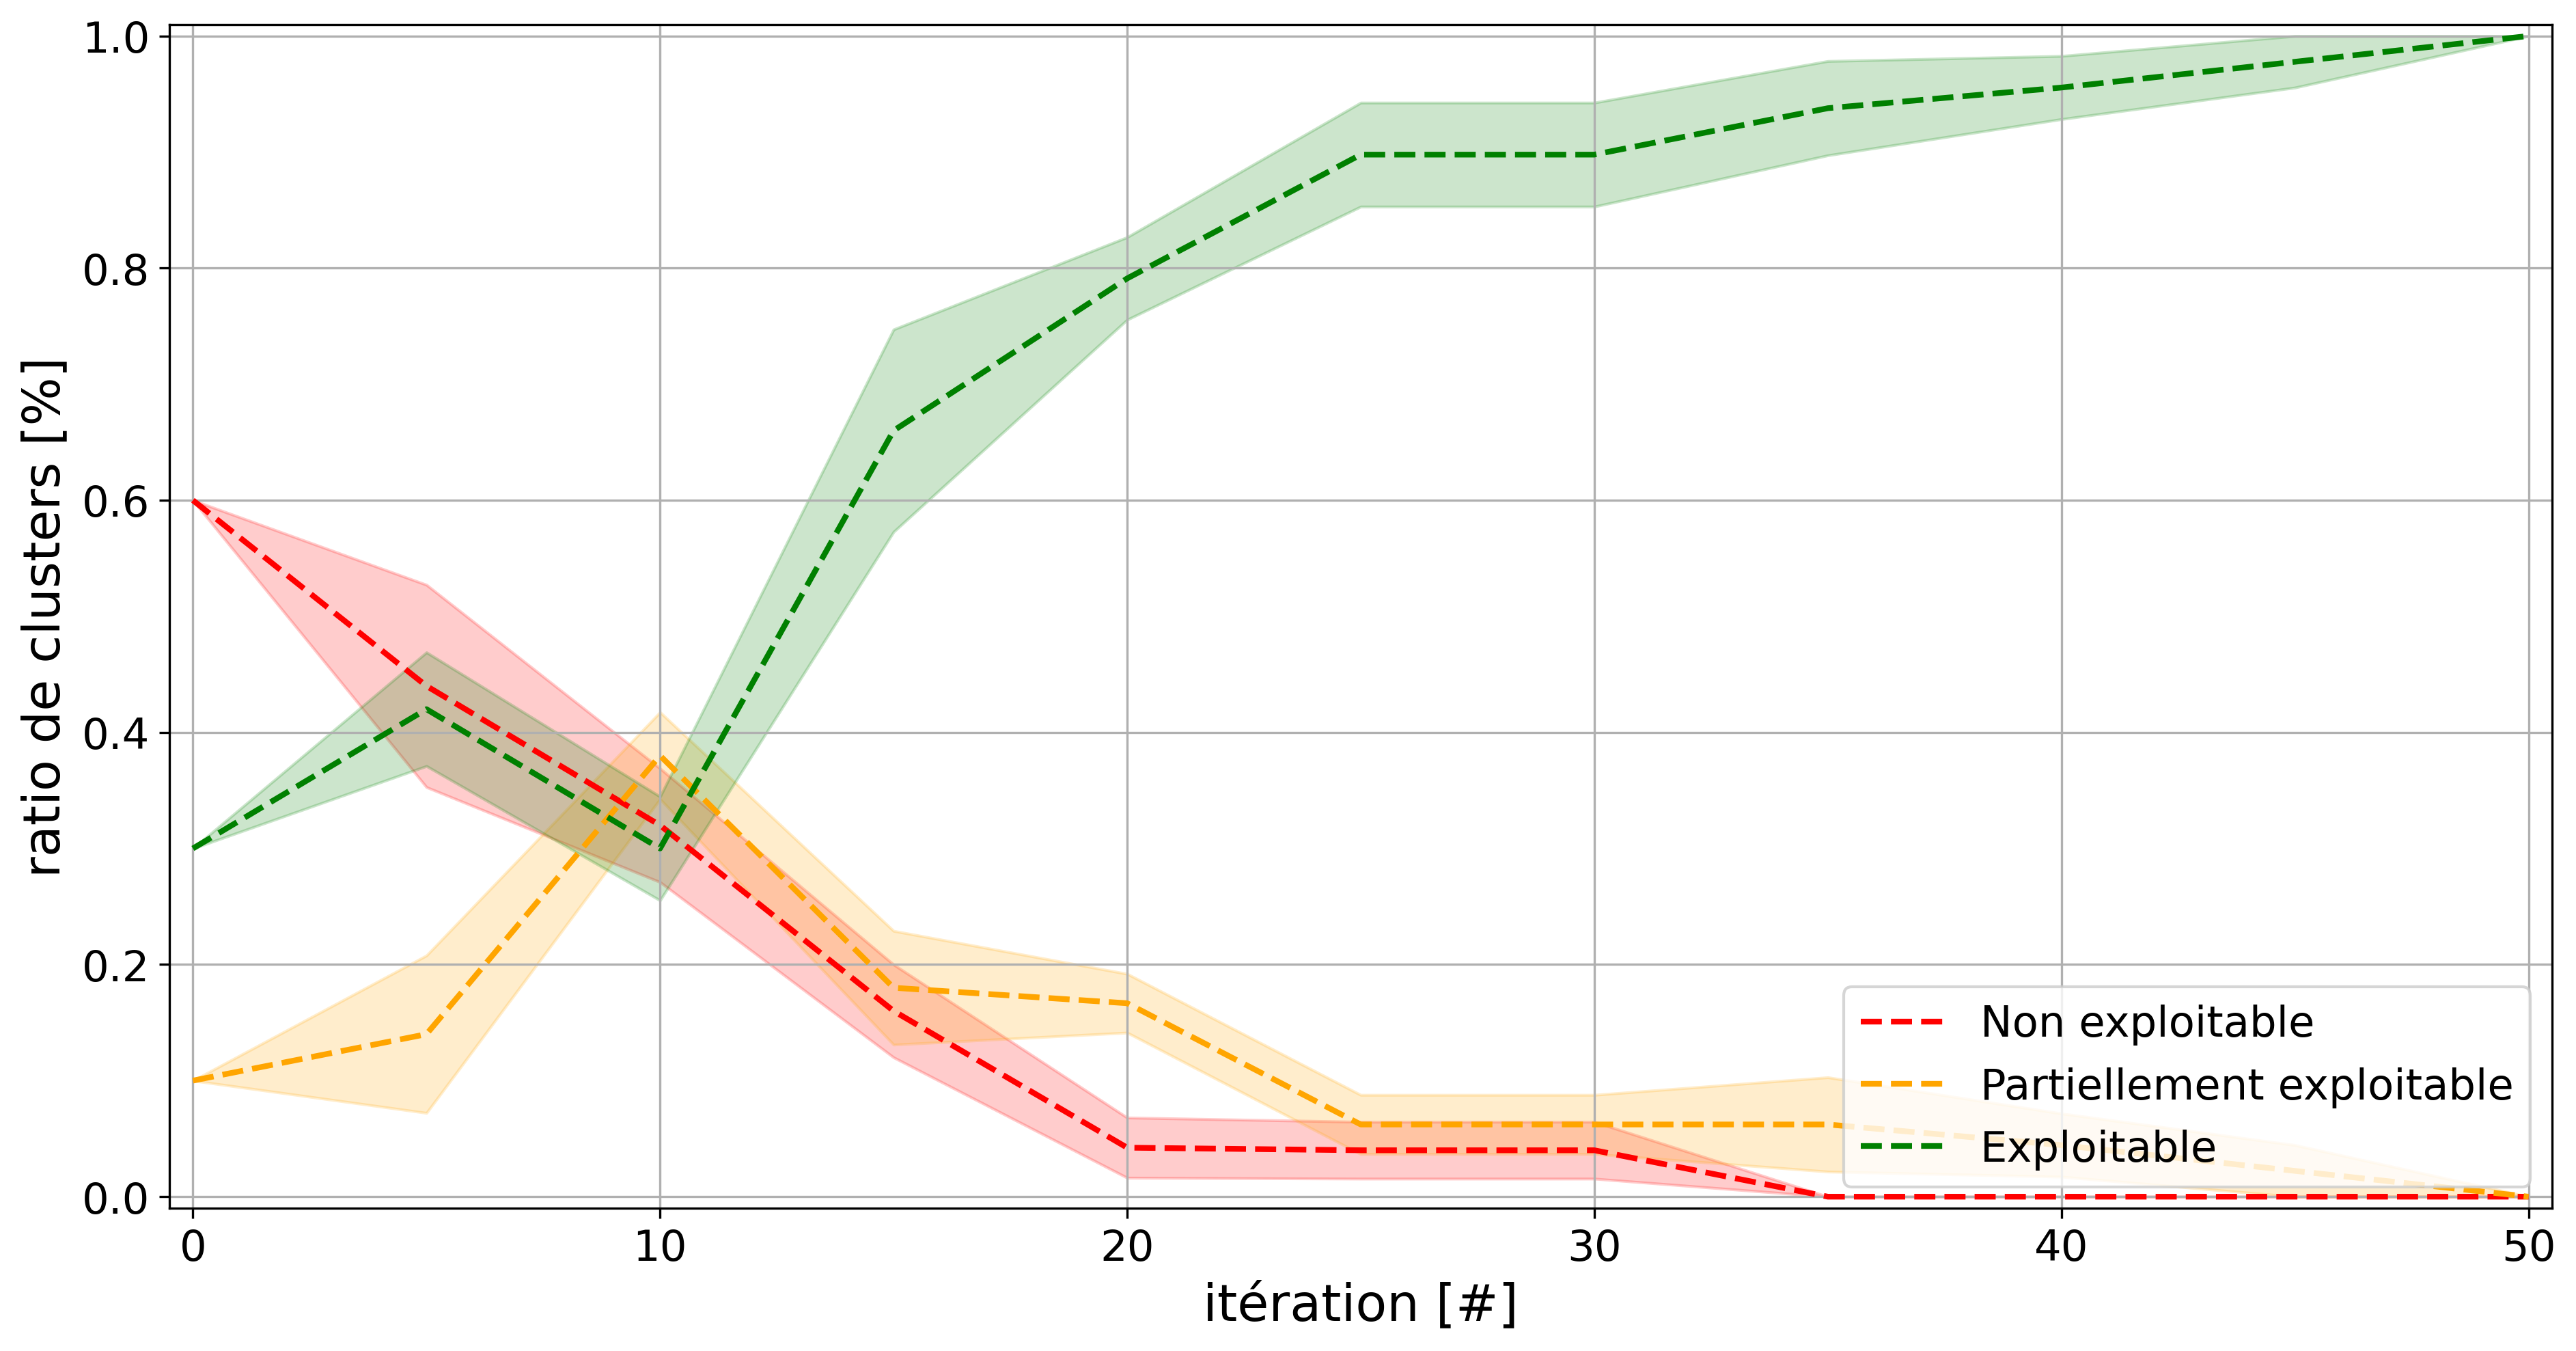
\includegraphics[width=0.95\textwidth]{figures/etude-pertinence-llm-check-clustering-annotation-favori}
				\caption{Évolution de la pertinence métier moyenne estimée manuellement au cours des itérations du résultat du \textit{clustering} interactif avec notre paramétrage favori.
				Cette pertinence, exprimée en proportion du nombre de \textit{clusters}, est retranscrite en trois niveaux : \texttt{exploitable} en vert, \texttt{partiellement exploitable} en orange, et \texttt{non exploitable} en rouge.}
				\label{figure:4.4.1-ETUDE-PERTINENCE-VERIFICATION-MANUELLE}
			\end{figure}


		%%% Discussion
		\subsubsection{Discussion}
		
			% Rappel de l'objectif.
			Cette première étude visait à observer comment un expert métier peut interpréter un résultat de \textit{clustering} proposé par notre méthode.
			
			% Remarques sur l'évolution de l'exploitabilité.
			Comme l'analyse n'a pu être faite que par un seul opérateur, nous ne nous attarderons pas sur la précision des taux d'exploitabilité des clusters.
			Nous pouvons déjà reconnaître que trois phases sont présentes :
			\begin{itemize}
				\item une première \textbf{phase exploratoire} (cf. itérations $0$ à $10$), où de premiers \textit{clusters} partiellement exploitables apparaissant.
				Ces derniers contiennent souvent une thématique bruitée ou quelques thématiques mal séparées, ce qui permet toutefois à l'expert de se faire une idée des thématiques contenu dans la collecte de données.
				Cependant, s'arrêter à ce stade demanderait beaucoup de travail manuel pour obtenir une base d'apprentissage opérationnelle ;
				\item une seconde \textbf{phase de consolidation} (cf. itérations $10$ à $25$), où les \textit{clusters} partiellement exploitable se raffinent.
				De plus en plus de \textit{clusters} bien définis naissent, avec une seul thématique et peu de bruits.
				Ces derniers pourraient être extraits et exploités en l'état ;
				\item une \textbf{phase de parachèvement} (cf. itérations après $25$), où la plupart des \textit{clusters} sont exploitables en l'état mais quelques-uns nécessitent encore du travail.
				Cette phase est la moins rentable car les derniers \textit{clusters} et points aberrants sont corrigés petit à petit, mais sans impact notable sur leur valeur métier. 
			\end{itemize}
			
			% Remaques expérience utilisateur : tâche complexe.
			Au cours de ces vérifications, il apparaît que la complexité réside dans l'analyse des \textit{clusters} partiellement exploitables.
			En effet, les clusters totalement exploitable ou totalement inexploitables sont souvent simples à identifier.
			les premiers se repèrent facilement, surtout quand ils sont déjà présents lors d'itérations précédentes (exemple de la classe \texttt{gestion\_sans\_contact}, présente dès l'itération $0$) ;
			les seconds, plutôt présents au début de la méthode, peuvent mélanger un grand nombre de thématique et s'apparenter rapidement à des \textit{clusters} poubelle.
			En revanche, les \textit{clusters} partiellement exploitables peuvent avoir des limites subjectives, alterant parfois l'avis de l'expert.
			
			% Remaques expérience utilisateur : tâche complexe.
			Pour aller plus loin, la difficulté de cette tâche est aussi dû aux contraintes suivantes :
			\begin{itemize}
				\item il faut être capable de maintenir en mémoire de grands ensembles de données ;
				\item il faut estimer la thématique principale à l'aide de données désordonnées ;
				\item il faut examiner la cohérence de cette thématique alors que le vocabulaire employé diffère ;
				\item il faut juger de l'importance du bruit contenu dans les \textit{clusters} ;
				\item il faut prendre du recul pour repérer la dispersion d'une thématique dans plusieurs \textit{clusters} ;
				\item ...
			\end{itemize}
			Tous ces facteurs peuvent donc nuire à la qualité, tant sur l'estimation de l'exploitabilité que sur le nommage des \textit{clusters}.
			
			% Remarques expérience utilisateur : impacts sur la qualité.
			Ainsi, nous déduisons aisément que l'expérience utilisateur proposée à l'expert métier n'est pas séduisante.
			Comme l'analyse de l'exploitabilité d'un \textit{cluster} semble être une tâche complexe, il semble inconcevable de demander sa réalisation sur tous les \textit{clusters} de toutes les itérations !
			De plus, sans aide supplémentaire et sans vis-à-vis pour se confronter à ses conclusions d'analyse, l'opérateur peut difficilement vérifier la cohérence et la reproductibilité de son travail.
			Il est donc nécessaire de considérer des pistes d'amélioration pour ne pas abandonner l'expert métier à lui-même dans cette tâche cruciale.
			
			% Conclusions et suggestion.
			Quelques pistes peuvent être étudiées pour accompagner l'opérateur :
			\begin{itemize}
				\item employer plusieurs experts pour valider par consensus leurs appréciation sur un résultat de \textit{clustering} : cette méthode est efficace pour rattraper les thématiques non identifiées et pour s'accorder sur la valeur d'un \textit{cluster} ;
				\item prémâcher le travail d'analyse en réalisant une étude linguistique des \textit{clusters}, et permettre ainsi d'identifier grossièrement les thématiques présentes en fonction du vocabulaire employé (cf. \textsc{Section~\ref{section:4.4.2-ETUDE-PERTINENCE-PATTERNS-LINGUISTIQUES}}) ;
				\item automatiser une partie du travail d'analyse en utilisant les capacités des larges modèles de langage (\textit{large language models}, \texttt{LLM}), afin d'alléger la charge de travail demandée aux experts métiers (cf. \textsc{Section~\ref{section:4.4.3-ETUDE-PERTINENCE-RESUME-AUTOMATIQUE}}).
			\end{itemize}
	
	
	%%%
	%%% Subsection 4.4.2: Etude des patterns linguistiques pertinents à l'aide de la \textit{Features Maximization}
	%%%
	\subsection{Étude des patterns linguistiques pertinents à l'aide de la Maximisation des Traits pour assister la vérification d'une base d'apprentissage}
	\label{section:4.4.2-ETUDE-PERTINENCE-PATTERNS-LINGUISTIQUES}
		
		% Objectif de l'expérience.
		Nous venons de conclure que la vérification manuelle d'un résultat de \textit{clustering} interactif est fonctionnelle, mais qu'elle souffre d'une très mauvaise expérience utilisateur.
		Afin d'améliorer cette aspect, une première idée consiste à mettre en valeur le vocabulaire caractéristique de chaque \textit{cluster} et d'examiner si ces informations sont utiles à l'appréciation de leur valeur métier.
	
		%%% Protocole expérimental.
		\subsubsection{Protocole expérimental}
			
			% Pseudo-code.
			Pour résumer le protocole expérimental adapté, vous pouvez vous référer au pseudo-code décrit dans \textsc{Algorithme~\ref{algorithm:4.4.2-ETUDE-PERTINENCE-PATTERNS-LINGUISTIQUES-PROTOCOLE}}.
			%
			\begin{algorithm}[!htb]
				\begin{algorithmic}[1]
					\Require jeux de données annotés (vérité terrain) de tailles différentes
					\State \textbf{initialisation (données)}: récupérer ou générer les données et la vérité terrain
					\State \textbf{initialisation (contraintes)}: créer une liste vide de contraintes
					\State \textbf{prétraitement}: supprimer le bruit dans les données avec \texttt{prep.simple}
					\State \textbf{vectorisation}: transformer les données en vecteurs avec \texttt{vect.tfidf}
					\State \textbf{clustering initial}: regrouper les données par similarité avec \texttt{clust.kmeans.cop}
					\State \textbf{évaluation manuelle}: juger de l'exploitabilité de chaque \textit{cluster}
					\Repeat
						\State \textbf{échantillonnage}: sélectionner de nouvelles contraintes à annoter
						\State \textbf{simulation d'annotation}: ajouter des contraintes avec \texttt{samp.closest.diff}
						\State \textbf{clustering}: regrouper les données par similarité avec \texttt{clust.kmeans.cop}
						\State \textbf{analyse linguistique}: déterminer le vocabulaire caractéristique de chaque cluster
						\State \textbf{évaluation semi-manuelle}: juger de l'exploitabilité de chaque \textit{cluster}
						\State \textbf{labellisation manuelle}: nommer chaque \textit{cluster} exploitable
					\Until{annotation de toutes les contraintes possibles}
					\State \textbf{analyse}: afficher l'évolution de l'exploitabilité de chaque itération de \textit{clustering}
					\Ensure discussion sur la complexité de la tâche et sur l'évolution de l'exploitabilité
				\end{algorithmic}
				\caption{Description en pseudo-code du protocole expérimental de l'étude des patterns linguistiques pertinents pour vérifier la valeur métier d'une base d'apprentissage.}
				\label{algorithm:4.4.2-ETUDE-PERTINENCE-PATTERNS-LINGUISTIQUES-PROTOCOLE}
			\end{algorithm}
			
			% Détails de l'expérience.
			Nous nous appuyons sur le même protocole que l'expérience précédente (cf. \textsc{Section~\ref{section:4.4.1-ETUDE-PERTINENCE-VERIFICATION-MANUELLE}}) : nous utilisons donc comme vérité terrain le jeu de données \texttt{Bank Cards (v1.0.0)}, nous réalisons $5$ tentatives complètes de la méthode du \textit{clustering} interactif utilisant notre paramétrage favori, et nous demandons toutes les $5$ itérations à un expert de qualifier les \textit{clusters} obtenus entre trois catégories (\textbf{exploitable}, \textbf{partiellement exploitable} et \textbf{non exploitable}).
			
			% Ajout de l'analyse linguistique.
			Cependant, avant de demander l'avis de l'expert, nous réalisons une analyse du vocabulaire employé.
			Pour cela, nous utilisons une sélection des patterns linguistiques pertinents basée sur la maximisation des traits (notée \texttt{FMC}, cf.~\cite{lamirel-etal:2017:novel-approach-feature}) : cette méthode permet de trouver les composantes vectorielle caractéristiques et discriminantes de chaque \textit{cluster} en attribuant un score à chaque couple $(\texttt{cluster}, \texttt{composante})$.
			Dans notre cas, en utilisant une vectorisation basée sur la fréquence du vocabulaire dans un document comme \textbf{TF-IDF} (\cite{sparck-jones:1972:statistical-interpretation-term}), nous pouvons déterminer les mots les plus représentatif de chaque \textit{cluster}.
			Ainsi, nous pouvons à la fois décrire chaque groupe de questions par une liste de mots clés caractéristiques, mais aussi surligner ces mots dans les questions à parcourir pour attirer l'attention de l'expert sur ce qui semble être statistiquement discriminant.
			
			% Description de l'évaluation semi-manuelle.
			Nous adaptons aussi la tâche de l'expert afin qu'il donne son avis sur chaque \textit{cluster} en répondant aux questions suivantes :
			\begin{itemize}
				\item est-ce que la liste des patterns linguistiques caractéristiques du \textit{cluster} est suffisamment complète pour permettre d'identifier une thématique principale \textbf{bien définie} ? (\textit{en effet, comment interpréter un cluster sans définition claire ?})
				\item est-ce que la liste des patterns linguistiques caractéristiques du \textit{cluster} identifie plusieurs thématiques ou bruits dans le \textit{cluster} ? (\textit{en effet, comment avoir de bonnes performances si la base d'apprentissage n'est pas fiable ?})
			\end{itemize}
			
			\begin{leftBarIdea}
				Nous pourrions aussi analyser l'impact ergonomique qu'apporte la mise en exergue des patterns linguistiques pertinents dans le texte de chaque \textit{cluster}.
				Une telle étude pourrait ainsi mesurer le gain de temps et de qualité par rapport à une vérification manuelle non assistée comme présentée en \textsc{Section~\ref{section:4.4.1-ETUDE-PERTINENCE-VERIFICATION-MANUELLE}}.
			\end{leftBarIdea}
			
			% Référence scripts.
			\begin{leftBarInformation}
				Les scripts de l'expérience, réalisés avec des \textit{notebooks} Python (\cite{van-rossum-drake:2009:python-reference-manual}), sont disponibles dans un dossier dédié de~\cite{schild:2021:cognitivefactory-interactiveclusteringcomparativestudy}.
				L'implémentation de la maximisation des traits est accessible ici dans~\cite{schild:2023:cognitivefactory-featuresmaximizationmetric}.
			\end{leftBarInformation}

		%%% Résultats
		\subsubsection{Résultats obtenus}
			
			% Axiome/Contraintes.
			\begin{leftBarWarning}
				Par manque de moyen, la relecture manuelle des \textit{clusters} n'a pas été réalisée.
				Nous présentons donc simplement quelques exemples d'analyses linguistiques réalisées grâce à la \texttt{FMC}.
			\end{leftBarWarning}
			
			% Description de deux cas d'études.
			Prenons quelques \textit{clusters} et suivons l'évolution de leur analyse linguistiques au cours des itérations.
			Nous nous référons aux tableaux ci-contre pour connaître le top $10$ des termes caractéristiques des différents \textit{clusters} ainsi qu'un extrait de questions issu de ces \textit{clusters} avec une mise en évidence des termes caractéristiques dans le texte.
			
			% Exemple d'un cluster qui est bien formé dès le début.
			D'abord, prenons l'exemple suivi dans la \textsc{Table~\ref{table:4.4.2-ETUDE-PERTINENCE-PATTERNS-LINGUISTIQUES-GESTION-SANS-CONTACT}}.
			Nous suivons ici l'évolution d'un \textit{cluster} bien formé dès l'itération $0$.
			En effet, il aisé de juger ce \textit{cluster} exploitable et d'en déduire sa thématique : le \textit{cluster} est de taille suffisante (plus de $45$ questions), son vocabulaire caractéristique est fourni ($36$ à $38$ patterns) et la liste des patterns mis en avant sont cohérents (\textit{sans contact}, \textit{paiement sans contact}, \texttt{activer le}, \textit{nfc}, ...).
			En parcourant son contenu, on arrive rapidement à associer sa thématique à la classe \texttt{gestion\_sans\_contact} de la vérité terrain.
			
			\begin{table}[!htb]
				\begin{center}
				\def\arraystretch{0.8}  % interligne
				\begin{tabular}{|c|l|l|}
				
					\hline
					% ENTETE DU TABLEAU
					\multicolumn{1}{|c|}{\shortstack[c]{
						Identification \\ du cluster
					}}
						& \multicolumn{1}{c|}{\shortstack[c]{
							Analyse linguistique \\ (avec la \texttt{FMC})
						}}
						& \multicolumn{1}{c|}{\shortstack[c]{
							Aperçu du cluster \\ (avec emphase)
						}}
						\tabularnewline
						\hline
					
					% Exemple 1.1:
					\multirow{10}{*}{\shortstack[c]{
						{ \footnotesize Tentative: $1$ } \\
						{ \footnotesize Itération: $0$ } \\
						{ \footnotesize Cluster: $0$ } \\
						{ \footnotesize Avis initial: } \\
						{ \footnotesize \color{colorDarkPastelGreen} \texttt{Exploitable} }
					}}
						& { \scriptsize - sans contact }
						& { \scriptsize - \textbf{activer le} moyen de \textbf{paiement nfc} \textbf{sur ma carte} gold }
						\tabularnewline
						
						& { \scriptsize - contact }
						& { \scriptsize - \textbf{enlever} le \textbf{mode} \textbf{sans contact} de ma carte }
						\tabularnewline
						
						& { \scriptsize - sans }
						& { \scriptsize - gerer le \textbf{mode} de \textbf{paiement nfc} \textbf{sur ma carte} }
						\tabularnewline
						
						& { \scriptsize - mode }
						& { \scriptsize - je souhaite gerer le \textbf{mode} nfc sur mes cartes bancaires }
						\tabularnewline
						
						& { \scriptsize - le mode }
						& { \scriptsize - l option \textbf{sans contact} \textbf{ne fonctionne pas} \textbf{sur ma carte} }
						\tabularnewline
						
						& { \scriptsize - sur ma carte }
						& { \scriptsize - modifier le \textbf{mode} \textbf{sans contact} }
						\tabularnewline
						
						& { \scriptsize - le sans contact }
						& { \scriptsize - modifier le \textbf{mode} nfc \textbf{sur ma carte} de paiement }
						\tabularnewline
						
						& { \scriptsize - le sans }
						& { \scriptsize - peut on annuler le paiement \textbf{sans contact} }
						\tabularnewline
						
						& { \scriptsize - paiement sans contact }
						& { \scriptsize - puis je \textbf{activer le} \textbf{sans contact} depuis l application }
						\tabularnewline
						
						& \multicolumn{1}{c|}{
							\scriptsize (Total: 36)
						}
						& \multicolumn{1}{c|}{
							\scriptsize (Total: 46)
						}
						\tabularnewline
						\hline
					
					% Exemple 1.2:
					\multirow{10}{*}{\shortstack[c]{
						{ \footnotesize Tentative: $1$ } \\
						{ \footnotesize Itération: $15$ } \\
						{ \footnotesize Cluster: $0$ } \\
						{ \footnotesize Avis initial: } \\
						{ \footnotesize \color{colorDarkPastelGreen} \texttt{Exploitable} }
					}}
						& { \scriptsize - sans contact }
						& { \scriptsize - \textbf{activer le} moyen de paiement \textbf{nfc} \textbf{sur ma} carte gold }
						\tabularnewline
						
						& { \scriptsize - contact }
						& { \scriptsize - \textbf{enlever} le \textbf{mode} \textbf{sans contact} de ma carte }
						\tabularnewline
						
						& { \scriptsize - sans }
						& { \scriptsize - gerer le \textbf{mode} de paiement \textbf{nfc} \textbf{sur ma} carte }
						\tabularnewline
						
						& { \scriptsize - sur ma }
						& { \scriptsize - je souhaite gerer le \textbf{mode} \textbf{nfc} sur mes cartes bancaires }
						\tabularnewline
						
						& { \scriptsize - mode }
						& { \scriptsize - l \textbf{option} \textbf{sans contact} ne fonctionne pas \textbf{sur ma} carte }
						\tabularnewline
						
						& { \scriptsize - le mode }
						& { \scriptsize - modifier le \textbf{mode} \textbf{sans contact} }
						\tabularnewline
						
						& { \scriptsize - sur ma carte }
						& { \scriptsize - modifier le \textbf{mode} \textbf{nfc} \textbf{sur ma carte de paiement} }
						\tabularnewline
						
						& { \scriptsize - nfc }
						& { \scriptsize - peut on annuler le paiement \textbf{sans contact} }
						\tabularnewline
						
						& { \scriptsize - le sans contact }
						& { \scriptsize - puis je \textbf{activer le} \textbf{sans contact} depuis l application }
						\tabularnewline
						
						& \multicolumn{1}{c|}{
							\scriptsize (Total: 38)
						}
						& \multicolumn{1}{c|}{
							\scriptsize (Total: 50)
						}
						\tabularnewline
						\hline
					
				\end{tabular}
				\end{center}
				\caption{Extrait de l'analyse linguistique de \textit{clusters} exploitables dès la première itération.
				Ces \textit{clusters} représentent la thématique \texttt{gestion\_sans\_contact} entre l'itération $0$ (initialisation) et l'itération $15$ (atteinte de la vérité terrain).
				La troisième colonne expose un aperçu du contenu des \textit{clusters} en mettant l'emphase sur les termes caractéristiques identifiés grâce à la \texttt{FMC}, et la deuxième colonne représente le top $10$ de ces termes les plus caractéristiques pour chaque \textit{cluster}.
				}
				\label{table:4.4.2-ETUDE-PERTINENCE-PATTERNS-LINGUISTIQUES-GESTION-SANS-CONTACT}
			\end{table}
			
			% Exemple d'un cluster qui se forme.
			Ensuite, prenons l'exemple décrit dans la \textsc{Table~\ref{table:4.4.2-ETUDE-PERTINENCE-PATTERNS-LINGUISTIQUES-DEBLOCAGE-CARTE-GESTION-CARTE-VIRTUELLE}}.
			A l'itération $0$, il est impossible d'exploiter ce \textit{cluster} : il n'y a que deux patterns mis en avant ne traitant pas d'une ma thématique, et les questions semblent toutes traiter de sujets différents.
			A l'itération $10$, le résultat semble un peu plus exploitable.
			Nous pouvons d'ailleurs déduire deux thématiques principales : la première, mise en avant par des patterns linguistiques de type "\textit{numero}", "\textit{online}", et "\textit{de carte virtuelle}", permet d'imaginer un sujet sur la gestion des numéro de cartes virtuelles ; la seconde, identifiée par les termes "\textit{débloquer}" et "\textit{réactiver}", oriente plutôt vers la création d'un thème pour débloquer une carte bancaire.
			Quelques bruits sont présent, mais ce \textit{cluster} à l'itération $10$ peut donc être associé aux classes \texttt{gestion\_carte\_virtuelle} et \texttt{deblocage\_carte}.
			Dès l'itération $15$, ces thématiques se séparent en deux clusters ($1$ et $4$) : nous pouvons les identifier à l'aide de leurs listes de termes bien fournies.
			
			\begin{table}[!htb]
				\begin{center}
				\def\arraystretch{0.8}  % interligne
				\begin{tabular}{|c|l|l|}
				
					\hline
					% ENTETE DU TABLEAU
					\multicolumn{1}{|c|}{\shortstack[c]{
						Identification \\ du cluster
					}}
						& \multicolumn{1}{c|}{\shortstack[c]{
							Analyse linguistique \\ (avec la \texttt{FMC})
						}}
						& \multicolumn{1}{c|}{\shortstack[c]{
							Aperçu du cluster \\ (avec emphase)
						}}
						\tabularnewline
						\hline
					
					% Exemple 2.1:
					\multirow{10}{*}{\shortstack[c]{
						{ \footnotesize Tentative: $1$ } \\
						{ \footnotesize Itération: $0$ } \\
						{ \footnotesize Cluster: $1$ } \\
						{ \footnotesize Avis initial: } \\
						{ \footnotesize \color{colorDarkPastelRed} \texttt{Non exploitable} }
					}}
						&
						& { \scriptsize - ai je le droit d avoir un decouvert bancaire }
						\tabularnewline
						
						&
						& { \scriptsize - bonjour pouvez vous debloquer ma carte merci }
						\tabularnewline
						
						&
						& { \scriptsize - carte bancaire avalee }
						\tabularnewline
						
						& { \scriptsize - carte avalee }
						& { \scriptsize - choisir une \textbf{nouvelle carte bancaire} }
						\tabularnewline
						
						& { \scriptsize - nouvelle carte bancaire }
						& { \scriptsize - comment signaler un vol de carte bleue }
						\tabularnewline
						
						& \multicolumn{1}{c|}{
							\scriptsize (Total: 2)
						}
						& { \scriptsize - diminuer le plafond d une carte gold }
						\tabularnewline
						
						& 
						& { \scriptsize - le rapatriement est il couvert par ma carte bancaire }
						\tabularnewline
						
						&
						& { \scriptsize - que faire pour activer une carte bancaire virtuelle }
						\tabularnewline
						
						&
						& { \scriptsize - quelle est ma situation financiere }
						\tabularnewline
						
						&
						& \multicolumn{1}{c|}{
							\scriptsize (Total: 157)
						}
						\tabularnewline
						\hline

					% Exemple 2.2:
					\multirow{10}{*}{\shortstack[c]{
						{ \footnotesize Tentative: $1$ } \\
						{ \footnotesize Itération: $10$ } \\
						{ \footnotesize Cluster: $2$ } \\
						{ \footnotesize Avis initial: } \\
						{ \footnotesize \color{colorCadmiumOrange} \texttt{Partiellement} } \\
						{ \footnotesize \color{colorCadmiumOrange} \texttt{exploitable} }
					}}
						& { \scriptsize - un numero }
						& { \scriptsize - activer les \textbf{achats} avec \textbf{un numero} \textbf{virtuel} }
						\tabularnewline
						
						& { \scriptsize - numero }
						& { \scriptsize - comment \textbf{debloquer ma} mastercard }
						\tabularnewline
						
						& { \scriptsize - de carte virtuelle }
						& { \scriptsize - comment \textbf{reactiver sa} carte }
						\tabularnewline
						
						& { \scriptsize - un numero de }
						& { \scriptsize - j aimerai \textbf{debloquer ma} carte svp }
						\tabularnewline
						
						& { \scriptsize - numero de carte }
						& { \scriptsize - pouvez vous \textbf{debloquer ma} carte }
						\tabularnewline
						
						& { \scriptsize - numero de }
						& { \scriptsize - obtenir une carte \textbf{online} }
						\tabularnewline
						
						& { \scriptsize - numeros }
						& { \scriptsize - ou en est ma situation financiere }
						\tabularnewline
						
						& { \scriptsize - debloquer ma }
						& { \scriptsize - ou puis je gerer mes \textbf{numero}s \textbf{virtuel}s }
						\tabularnewline
						
						& { \scriptsize - débloquer ma carte }
						& { \scriptsize - supprimer \textbf{une carte virtuelle} }
						\tabularnewline
						
						& \multicolumn{1}{c|}{
							\scriptsize (Total: 25)
						}
						& \multicolumn{1}{c|}{
							\scriptsize (Total: 80)
						}
						\tabularnewline
						\hline

					% Exemple 2.3a:
					\multirow{10}{*}{\shortstack[c]{
						{ \footnotesize Tentative: $1$ } \\
						{ \footnotesize Itération: $15$ } \\
						{ \footnotesize Cluster: $2$ } \\
						{ \footnotesize Avis initial: } \\
						{ \footnotesize \color{colorDarkPastelGreen} \texttt{Exploitable} }
					}}
						
						& { \scriptsize - virtuelle }
						& { \scriptsize - \textbf{activer les} \textbf{achats} avec \textbf{un numero} \textbf{virtuel} }
						\tabularnewline
						
						& { \scriptsize - carte virtuelle }
						& { \scriptsize - comment consulter \textbf{ses} \textbf{numero}s de carte \textbf{virtuelle} }
						\tabularnewline
						
						& { \scriptsize - un numero }
						& { \scriptsize - comment obtenir \textbf{un numero} de carte \textbf{virtuelle} }
						\tabularnewline
						
						& { \scriptsize - numero }
						& { \scriptsize - comment supprimer \textbf{un numero} de carte \textbf{online} }
						\tabularnewline
						
						& { \scriptsize - de carte virtuelle }
						& { \scriptsize - \textbf{creer} une carte bancaire \textbf{virtuelle} }
						\tabularnewline
						
						& { \scriptsize - un numero de }
						& { \scriptsize - faire un achat avec \textbf{un numero} de carte \textbf{online} }
						\tabularnewline
						
						& { \scriptsize - numero de carte }
						& { \scriptsize - j aimerai utiliser une carte \textbf{virtuelle} }
						\tabularnewline
						
						& { \scriptsize - numero de }
						& { \scriptsize - ou peut on gerer \textbf{ses} \textbf{numero}s \textbf{virtuel}s }
						\tabularnewline
						
						& { \scriptsize - numeros }
						& { \scriptsize - supprimer \textbf{un numero} de carte \textbf{virtuel} }
						\tabularnewline
						
						& \multicolumn{1}{c|}{
							\scriptsize (Total: 34)
						}
						& \multicolumn{1}{c|}{
							\scriptsize (Total: 49)
						}
						\tabularnewline
						\hline

					% Exemple 3b:
					\multirow{10}{*}{\shortstack[c]{
						{ \footnotesize Tentative: $1$ } \\
						{ \footnotesize Itération: $15$ } \\
						{ \footnotesize Cluster: $4$ } \\
						{ \footnotesize Avis initial: } \\
						{ \footnotesize \color{colorDarkPastelGreen} \texttt{Exploitable} }
					}}
						
						& { \scriptsize - reactiver }
						& { \scriptsize - bonjour pouvez vous \textbf{debloquer} ma carte merci }
						\tabularnewline
						
						& { \scriptsize - debloquer }
						& { \scriptsize - comment \textbf{deverrouiller} sa carte }
						\tabularnewline
						
						& { \scriptsize - debloquer ma }
						& { \scriptsize - comment reutiliser une carte bancaire \textbf{bloquee} }
						\tabularnewline
						
						& { \scriptsize - debloquer ma carte }
						& { \scriptsize - \textbf{debloquer} sa carte apres trois \textbf{mauvais} codes }
						\tabularnewline
						
						& { \scriptsize - bloquee }
						& { \scriptsize - j ai besoin de \textbf{deverrouiller} ma carte de paiement }
						\tabularnewline
						
						& { \scriptsize - reactiver sa }
						& { \scriptsize - j ai retrouve ma carte puis je la \textbf{reactiver} }
						\tabularnewline
						
						& { \scriptsize - reactiver ma }
						& { \scriptsize - je souhaite \textbf{debloquer} ma carte bleue }
						\tabularnewline
						
						& { \scriptsize - deverrouiller }
						& { \scriptsize - pouvez vous \textbf{debloquer} ma carte }
						\tabularnewline
						
						& { \scriptsize - reactiver sa carte }
						& { \scriptsize - \textbf{reactiver} une carte suspendue }
						\tabularnewline
						
						& \multicolumn{1}{c|}{
							\scriptsize (Total: 24)
						}
						& \multicolumn{1}{c|}{
							\scriptsize (Total: 48)
						}
						\tabularnewline
						\hline
					
				\end{tabular}
				\end{center}
				\caption{Extrait de l'analyse linguistique de \textit{clusters} évoluant de non exploitables à exploitables.
				Ces \textit{clusters} représentent la conception des thématiques \texttt{gestion\_carte\_virtuelle} et \texttt{deblocage\_carte}, entre l'itération $0$ (initialisation) et l'itération $15$ (atteinte de la vérité terrain).
				La troisième colonne expose un aperçu du contenu des \textit{clusters} en mettant l'emphase sur les termes caractéristiques identifiés grâce à la \texttt{FMC}, et la deuxième colonne représente le top $10$ de ces termes les plus caractéristiques pour chaque \textit{cluster}.
				}
				\label{table:4.4.2-ETUDE-PERTINENCE-PATTERNS-LINGUISTIQUES-DEBLOCAGE-CARTE-GESTION-CARTE-VIRTUELLE}
			\end{table}

		%%% Discussion
		\subsubsection{Discussion}
		
			% Rappel de l'objectif.
			Cette seconde étude avait pour objectif de proposer une assistance à la vérification manuelle des \textit{clusters} par un expert métier afin d'en qualifier la pertinence métier.
			Pour cela, nous avons choisi une analyse linguistique à l'aide de la maximisation de traits pour mettre en avant les mots représentatif et discriminants de chaque groupe de questions.
			Nous discutons ici de l'intérêt d'une telle analyse.
			
			% La FMC est très utile pour distinguer les clusters exploitables.
			Tout d'abord, concernant les \textit{clusters} jugés exploitables, nous constatons que la \texttt{FMC} permet d'identifier aisément la thématique principale.
			C'est le cas dans les exemples présentés dans les \textsc{Table~\ref{table:4.4.2-ETUDE-PERTINENCE-PATTERNS-LINGUISTIQUES-GESTION-SANS-CONTACT}} et \textsc{Table~\ref{table:4.4.2-ETUDE-PERTINENCE-PATTERNS-LINGUISTIQUES-DEBLOCAGE-CARTE-GESTION-CARTE-VIRTUELLE}}), où les thématiques sont bien représentées par leurs patterns (\texttt{gestion\_sans\_contact} avec "\textit{mode}", "\textit{sans}", "\textit{contact}", "\textit{nfc}" ; \texttt{gestion\_carte\_virtuelle} avec "\textit{numero}", "\textit{virtuel}", "\textit{online}" ; \texttt{deblocage\_carte} avec "\textit{debloquer}", "\textit{deverrouiller}", "\textit{carte}")
			De plus, la présence des différentes variantes d'un même pattern (avec ses pluriels, au sein d'un groupe de termes, ...) permet de rapidement d'intégrer le champ lexical présent, aidant ainsi à interpréter le \textit{cluster} comme probablement exploitable.
			
			% La FMC est utile : on distingue les thématiques d'un cluster partiellement exploitable.
			Les thématiques présentent dans les \textit{clusters} partiellement exploitables sont aussi identifiables grâce à la \texttt{FMC}, mais à moindre mesure.
			En effet, comme plusieurs thématiques se mélangent, l'ensemble de termes caractéristiques est aussi plus hétérogène, des variantes ne sont pas identifiées, et des patterns dénués de sens peuvent être mis en avant.
			Par exemple, dans le \textit{cluster} $2$ de la tentative $1$ à l'itération $0$, deux classes sont présentes avec leurs termes caractéristiques (\texttt{consultation\_solde} avec "\textit{solde}" et "\textit{compte}" ; \texttt{gestion\_carte\_virtuelle} avec "\textit{carte virtuelle}" et "\textit{numero}"), mais certains termes quelconque sont pourtant sont présentés comme représentatifs ("\textit{de mes}", "\textit{avec un}") et d'autres termes intéressants ne sont pas identifiés ("\textit{compte}" et "\textit{numeros}" ne sont présents qu'au singulier).
			Ces petits indices peuvent donc aiguiller l'expert sur des ajustements nécessaires ou un \textit{cluster} réalisé sur des bases fragiles.
			
			% La FMC est utile : on ne distingue pas de thématiques dans un cluster inexploitable.
			Enfin, en ce qui concerne les \textit{clusters} jugés non exploitables, la \texttt{FMC} permet de confirmer leur manque de cohérence (pour le \textit{cluster} $1$ de la tentative $2$ à l'itération $0$ : "\textit{carte gold}", "\textit{numeros virtuels}", "\textit{découvert bancaire}", "\textit{carte paiement differe}", ...) ou leur absence de valeur métier (seulement $2$ termes caractéristiques pour le \textit{cluster} $1$ de la tentative $1$ à l'itération $0$).
			Nous pouvons aussi constater que les termes estimés comme caractéristiques pour ces \textit{clusters} non exploitables sont souvent des groupes de mots trop spécifiques (dans notre dernier exemple : "\textit{numeros virtuels}" uniquement au pluriel), ce qui est plutôt caractéristique de termes qui distinguent le \textit{cluster} des autres mais qui ne l'identifient pas (voir~\cite{lamirel-etal:2017:novel-approach-feature} pour comprendre la balance entre \textit{Features Recall} (identification) et \textit{Features Predominance} (discrimination)).
			
			% Remaques expérience utilisateur : toujours une tâche complexe.
			Cependant, une telle approche pour qualifier les \textit{clusters} risque de ne pas répondre à nos attentes en l'état.
			D'une part, certains problèmes identifiés dans la sous-section précédente (\ref{section:4.4.1-ETUDE-PERTINENCE-VERIFICATION-MANUELLE}) sur une approche purement manuelle subsistent.
			Entre autres, malgré une abstraction des \textit{clusters} par leur termes les plus caractéristiques (cf. deuxième colonne dans les \textsc{Table~\ref{table:4.4.2-ETUDE-PERTINENCE-PATTERNS-LINGUISTIQUES-GESTION-SANS-CONTACT}} et \textsc{Table~\ref{table:4.4.2-ETUDE-PERTINENCE-PATTERNS-LINGUISTIQUES-DEBLOCAGE-CARTE-GESTION-CARTE-VIRTUELLE}}) et une mise en exergue dans le texte (cf. troisième colonne de ces tableaux), il faut toujours parcourir l'ensemble de ces données pour juger de la pertinence métier, ce qui reste une tâche chronophage s'il faut la réaliser à chaque itération.
			
			% Remaques expérience utilisateur : affiner les résultats
			D'autre part, les résultats remontés par l'analyse linguistiques pourraient être davantage affinés et mis en avant pour faciliter leur interprétation.
			Par exemple, les mots pourraient être réduits à leur forme racine (lemmatisation) pour éviter de considérer les nombreuses variations possibles (formes conjuguées, pluriels, ...)et les mots vides (stopwords) pourraient être supprimés pour accentuer l'absence de termes caractéristiques des \textit{clusters} inexploitables.
			En ce qui concerne l'affichage des patterns identifiés dans les textes, un code couleur peut être introduit pour faciliter la lecture, avec un vert pour les patterns associés au \textit{cluster} courant et un rouge pour ceux associés aux autres \textit{cluster}.
			Des nuances de couleurs pourraient même être utilisées en fonction de la prépondérance d'un terme pour chaque \textit{cluster}.
			L'exemple ci-dessous (issu du \textit{cluster} $0$ de la tentative $1$ à l'itération $0$) permet de se faire un aperçu de l'intérêt de cette coloration : on distingue facilement que le \textit{cluster} traite des paiements sans contact (\texttt{NFC}) mais que les cartes \textit{Visa} ont dû être regroupées au sein d'un autre \textit{cluster}.

			\begin{leftBarExamples}
				\begin{quote}
					« \textit{ est ce que le \textcolor{colorDarkPastelGreen}{\textbf{mode}} de \textcolor{colorDarkPastelGreen}{\textbf{paiement nfc}} est disponible \textcolor{colorDarkPastelGreen}{\textbf{sur ma carte}} \textcolor{colorDarkPastelRed}{\textbf{visa}} } »
				\end{quote}
			\end{leftBarExamples}
			
			% Remaques expérience utilisateur : tâche hors compétences d'un expert.
			Pour finir, il est probable qu'une analyse linguistique soit trop éloignée des compétences réelles des experts : ces derniers disposent de connaissances sur leur domaine métier (dans notre cas, des sujets concernant la banque, l’assurance et la finance), mais ne disposent pas forcément d'aptitudes permettant d'examiner les nuances linguistiques présentes dans un \textit{cluster}, ni l'impact de la prépondérance des pluriels, des bigrams, des mots vides de sens, ...
		
			% Note de l'auteur.
			\begin{leftBarAuthorOpinion}
				% Expérience personnelle.
				Nous utilisons notre expérience personnelle pour avancer cet avis.
				En effet, lors de précédents travaux industriels (non publiés), nous avons réalisé une modélisation thématique (\textit{topic modeling}) sur des corps de mail en utilisant la \texttt{LDA} (\cite{blei-etal:2003:latent-dirichlet-allocation}).
				Comme il est coutume, nous avons réaliser une abstraction en énumérant le vocabulaire employé par chaque \textit{topic}.
				Puis, nous avons fait intervenir des experts métiers afin d'estimer la valeur de chaque \textit{topic}, de les raffiner, et de les nommer grâce aux abstractions réalisées.
				Toutefois, nous avons constaté que les expert intervenants dans ce projet avaient du mal à manipuler de telles abstractions, notamment car ils n'arrivaient pas à se projeter sur les \textit{topic} peu ou pas exploitable.
				Au final, les experts ont préféré modéliser manuellement le corpus de mail, sans utiliser les résultats de la \texttt{LDA}.
				
				% Avis sur cette expérience personnelle.
				Une partie de cet échec est probablement lié à l'utilisation en tant que telle de la \texttt{LDA} (peu d'interactivité entre l'expert et l'algorithme de modélisation), mais nous avons aussi eu des retours directs des experts sur leur difficulté à utiliser des champs lexicaux pour juger de la qualité et de la cohérence d'une modélisation.
				Ainsi, même si une abstraction linguistique semble sémantiquement pertinente, il se peut que les intervenants du projet ne soient pas à l'aise avec son utilisation.
				Une étude spécifique à ce sujet pourrait vérifier ce ressenti.
			\end{leftBarAuthorOpinion}
			
			% Conclusions et suggestion.
			Pour conclure, nous retenons que l'analyse linguistique est pleine de potentielle et qu'elle permet de mettre en exergue des mots importants lors de l'affichage du contenu des clusters. Toutefois, nous avons des doutes sur l'expérience utilisateur d'une telle approche pour des experts métier qui ne sont pas des experts en linguistique, et nous anticipons .
			De fait, si une approche linguistique est trop abstraite pour qualifier un \textit{cluster}, nous nous intéressons à une approche plus pragmatique pour identifier sa thématique principale (cf. \textsc{Section~\ref{section:4.4.3-ETUDE-PERTINENCE-RESUME-AUTOMATIQUE}}).
	
	
	%%%
	%%% Subsection 4.4.3: Etude d'un résumé automatique des \textit{clusters} à l'aide d'un large modèle de langage.
	%%%
	\subsection{Étude d'un résumé automatique des \textit{clusters} à l'aide d'un large modèle de langage}
	\label{section:4.4.3-ETUDE-PERTINENCE-RESUME-AUTOMATIQUE}
		
		% Objectif de l'expérience.
		Comme nous l'avons vu dans la section précédente, une analyse linguistique peut paraître trop abstraite pour un expert métier.
		Nous nous intéressons donc à un moyen de simplifier l'identification de thématiques dans un \textit{cluster}, et envisageons l'automatisation de cette tâche en utilisant les capacités d'un large modèle de langage (\texttt{LLM}).
		En effet, plusieurs de ces modèles ont montré leur efficacité sur les tâches de résumé de documents (\cite{zhang-etal:2019:pegasus-pretraining-extracted}, \cite{lewis-etal:2019:bart-denoising-sequencetosequence}, \cite{radford-etal:2019:language-models-are}, \cite{brown-etal:2020:language-models-are}), une fonctionnalité que nous allons adapter\footnote{Nous nous inspirons notamment de~\cite{alammar-grefenstette:2022:cohere-sandbox} qui propose un boîte à outils en Python permettant de nommer des \textit{topics} en utilisant \texttt{BERT}.} et étudier ici.
	
		%%% Protocole expérimental.
		\subsubsection{Protocole expérimental}
			
			% Pseudo-code.
			Pour résumer le protocole expérimental adapté, vous pouvez vous référer au pseudo-code décrit dans \textsc{Algorithme~\ref{algorithm:4.4.3-ETUDE-PERTINENCE-RESUME-AUTOMATIQUE-PROTOCOLE}}.
			%
			\begin{algorithm}[!htb]
				\begin{algorithmic}[1]
					\Require jeux de données annotés (vérité terrain) de tailles différentes
					\State \textbf{initialisation (données)}: récupérer ou générer les données et la vérité terrain
					\State \textbf{initialisation (contraintes)}: créer une liste vide de contraintes
					\State \textbf{prétraitement}: supprimer le bruit dans les données avec \texttt{prep.simple}
					\State \textbf{vectorisation}: transformer les données en vecteurs avec \texttt{vect.tfidf}
					\State \textbf{clustering initial}: regrouper les données par similarité avec \texttt{clust.kmeans.cop}
					\State \textbf{évaluation manuelle}: juger de l'exploitabilité de chaque \textit{cluster}
					\Repeat
						\State \textbf{échantillonnage}: sélectionner de nouvelles contraintes à annoter
						\State \textbf{simulation d'annotation}: ajouter des contraintes avec \texttt{samp.closest.diff}
						\State \textbf{clustering}: regrouper les données par similarité avec \texttt{clust.kmeans.cop}
						\State \textbf{résumé automatique}: utiliser un modèle de langue pour identifier les thématiques
						\State \textbf{évaluation semi-manuelle}: juger de l'exploitabilité de chaque \textit{cluster}
						\State \textbf{labellisation manuelle}: nommer chaque \textit{cluster} exploitable
					\Until{annotation de toutes les contraintes possibles}
					\State \textbf{analyse}: afficher l'évolution de l'exploitabilité de chaque itération de \textit{clustering}
					\Ensure discussion sur la complexité de la tâche et sur l'évolution de l'exploitabilité
				\end{algorithmic}
				\caption{Description en pseudo-code du protocole expérimental de l'étude d'un résumé automatique des \textit{clusters} à l'aide d'un modèle de langue pour vérifier la valeur métier d'une base d'apprentissage.}
				\label{algorithm:4.4.3-ETUDE-PERTINENCE-RESUME-AUTOMATIQUE-PROTOCOLE}
			\end{algorithm}
			
			% Détails de l'expérience.
			Nous nous appuyons sur le même protocole que l'expérience précédente (cf. \textsc{Section~\ref{section:4.4.1-ETUDE-PERTINENCE-VERIFICATION-MANUELLE}}) : nous utilisons donc comme vérité terrain le jeu de données \texttt{Bank Cards (v1.0.0)}, nous réalisons $5$ tentatives complètes de la méthode du \textit{clustering} interactif utilisant notre paramétrage favori, et nous demandons toutes les $5$ itérations à un expert de qualifier les \textit{clusters} obtenus entre trois catégories (\textbf{exploitable}, \textbf{partiellement exploitable} et \textbf{non exploitable}).
			
			% Ajout d'un résumé automatique.
			Cependant, avant de demander l'avis de l'expert, nous utilisons un large modèle de langage pour résumer automatiquement le contenu du \textit{cluster} à analyser.
			Pour cela, nous utilisons le modèle \texttt{gpt-3.5-turbo} mis à disposition par \texttt{OpenAI}\todo{footenote avec détails sur OpenAI ?}.
			Le \textit{prompt} du modèle, adapté à l'usage de notre jeu de données, est composé de trois parties :
			\begin{itemize}
				\item un \textbf{contexte d'utilisation}, destiné à centrer les réponses sur le domaine général traité : « \textit{Tu es un expert des secteurs banque, assurance et finance.} » ;
				\item une \textbf{description de la tâche} avec les contraintes de restitution : « \textit{Résume-moi en une phrase la thématique traitée dans les textes suivants :} » ;
				\item les \textbf{données} du \textit{cluster}, sous la forme d'une énumération. Si la taille maximale du \textit{prompt} ne peut pas prendre en compte l'ensemble des données du \textit{cluster}, il est possible de ne prendre qu'un échantillon.
			\end{itemize}
			À l'aide de ces résumés, nous pouvons ainsi prémâcher le travail de l'expert en mettant en avant une synthèse des information contenus dans chaque \textit{cluster}.
			
			% Description de l'évaluation semi-manuelle.
			Nous adaptons aussi la tâche de l'expert afin qu'il donne son avis sur chaque \textit{cluster} en répondant aux questions suivantes :
			\begin{itemize}
				\item est-ce que le résumé est suffisamment précis pour identifier une thématique principale \textbf{bien définie} dans le \textit{cluster} ? (\textit{en effet, comment interpréter un cluster sans définition claire ?})
				\item est-ce que le résumé identifie plusieurs thématiques ou bruits dans le \textit{cluster} ? (\textit{en effet, comment avoir de bonnes performances si la base d'apprentissage n'est pas fiable ?})
			\end{itemize}
			
			% Référence scripts.
			\begin{leftBarInformation}
				Les scripts de l'expérience, réalisés avec des \textit{notebooks} Python (\cite{van-rossum-drake:2009:python-reference-manual}), sont disponibles dans un dossier dédié de~\cite{schild:2021:cognitivefactory-interactiveclusteringcomparativestudy}.
				L'appel à un modèle de langue, sous la forme d'un appel API, se fait grâce à la librairie \texttt{openai}.
			\end{leftBarInformation}

		%%% Résultats
		\subsubsection{Résultats obtenus}
			
			% Axiome/Contraintes.
			\begin{leftBarWarning}
				Par manque de personnes aptes à qualifier le jeu de données utilisé, les annotations réalisées dans cette étude n'ont pu être faites que par un seul annotateur.
				Malgré cette contrainte, nous supposons que la réalisation de l'analyse sur $5$ tentatives différentes de la méthode permet de limiter les biais et de discuter des tendances générales.
			\end{leftBarWarning}
		
			% Description statistiques.
			La \textsc{Figure~\ref{figure:4.4.3-ETUDE-PERTINENCE-RESUME-AUTOMATIQUE}} met en avant l'évolution de le pertinence moyenne estimée par l'opérateur sur la base des résumés automatiques des \textit{clusters}.
			Comme lors de l'analyse manuelle (cf. \textsc{Section~\ref{section:4.4.1-ETUDE-PERTINENCE-VERIFICATION-MANUELLE}}), il est normal de retrouver une tendance générale à la diminution du nombre de \textit{clusters} inexploitables au profit de \textit{clusters} exploitables.
			La différence principale réside dans l'absence du pic de croissance du nombre de \textit{clusters} partiellement exploitables, dont l'apogée était précédemment situé à l'itération $10$.
			
			% Figure.
			%
			\begin{figure}[!htb]
				\centering
				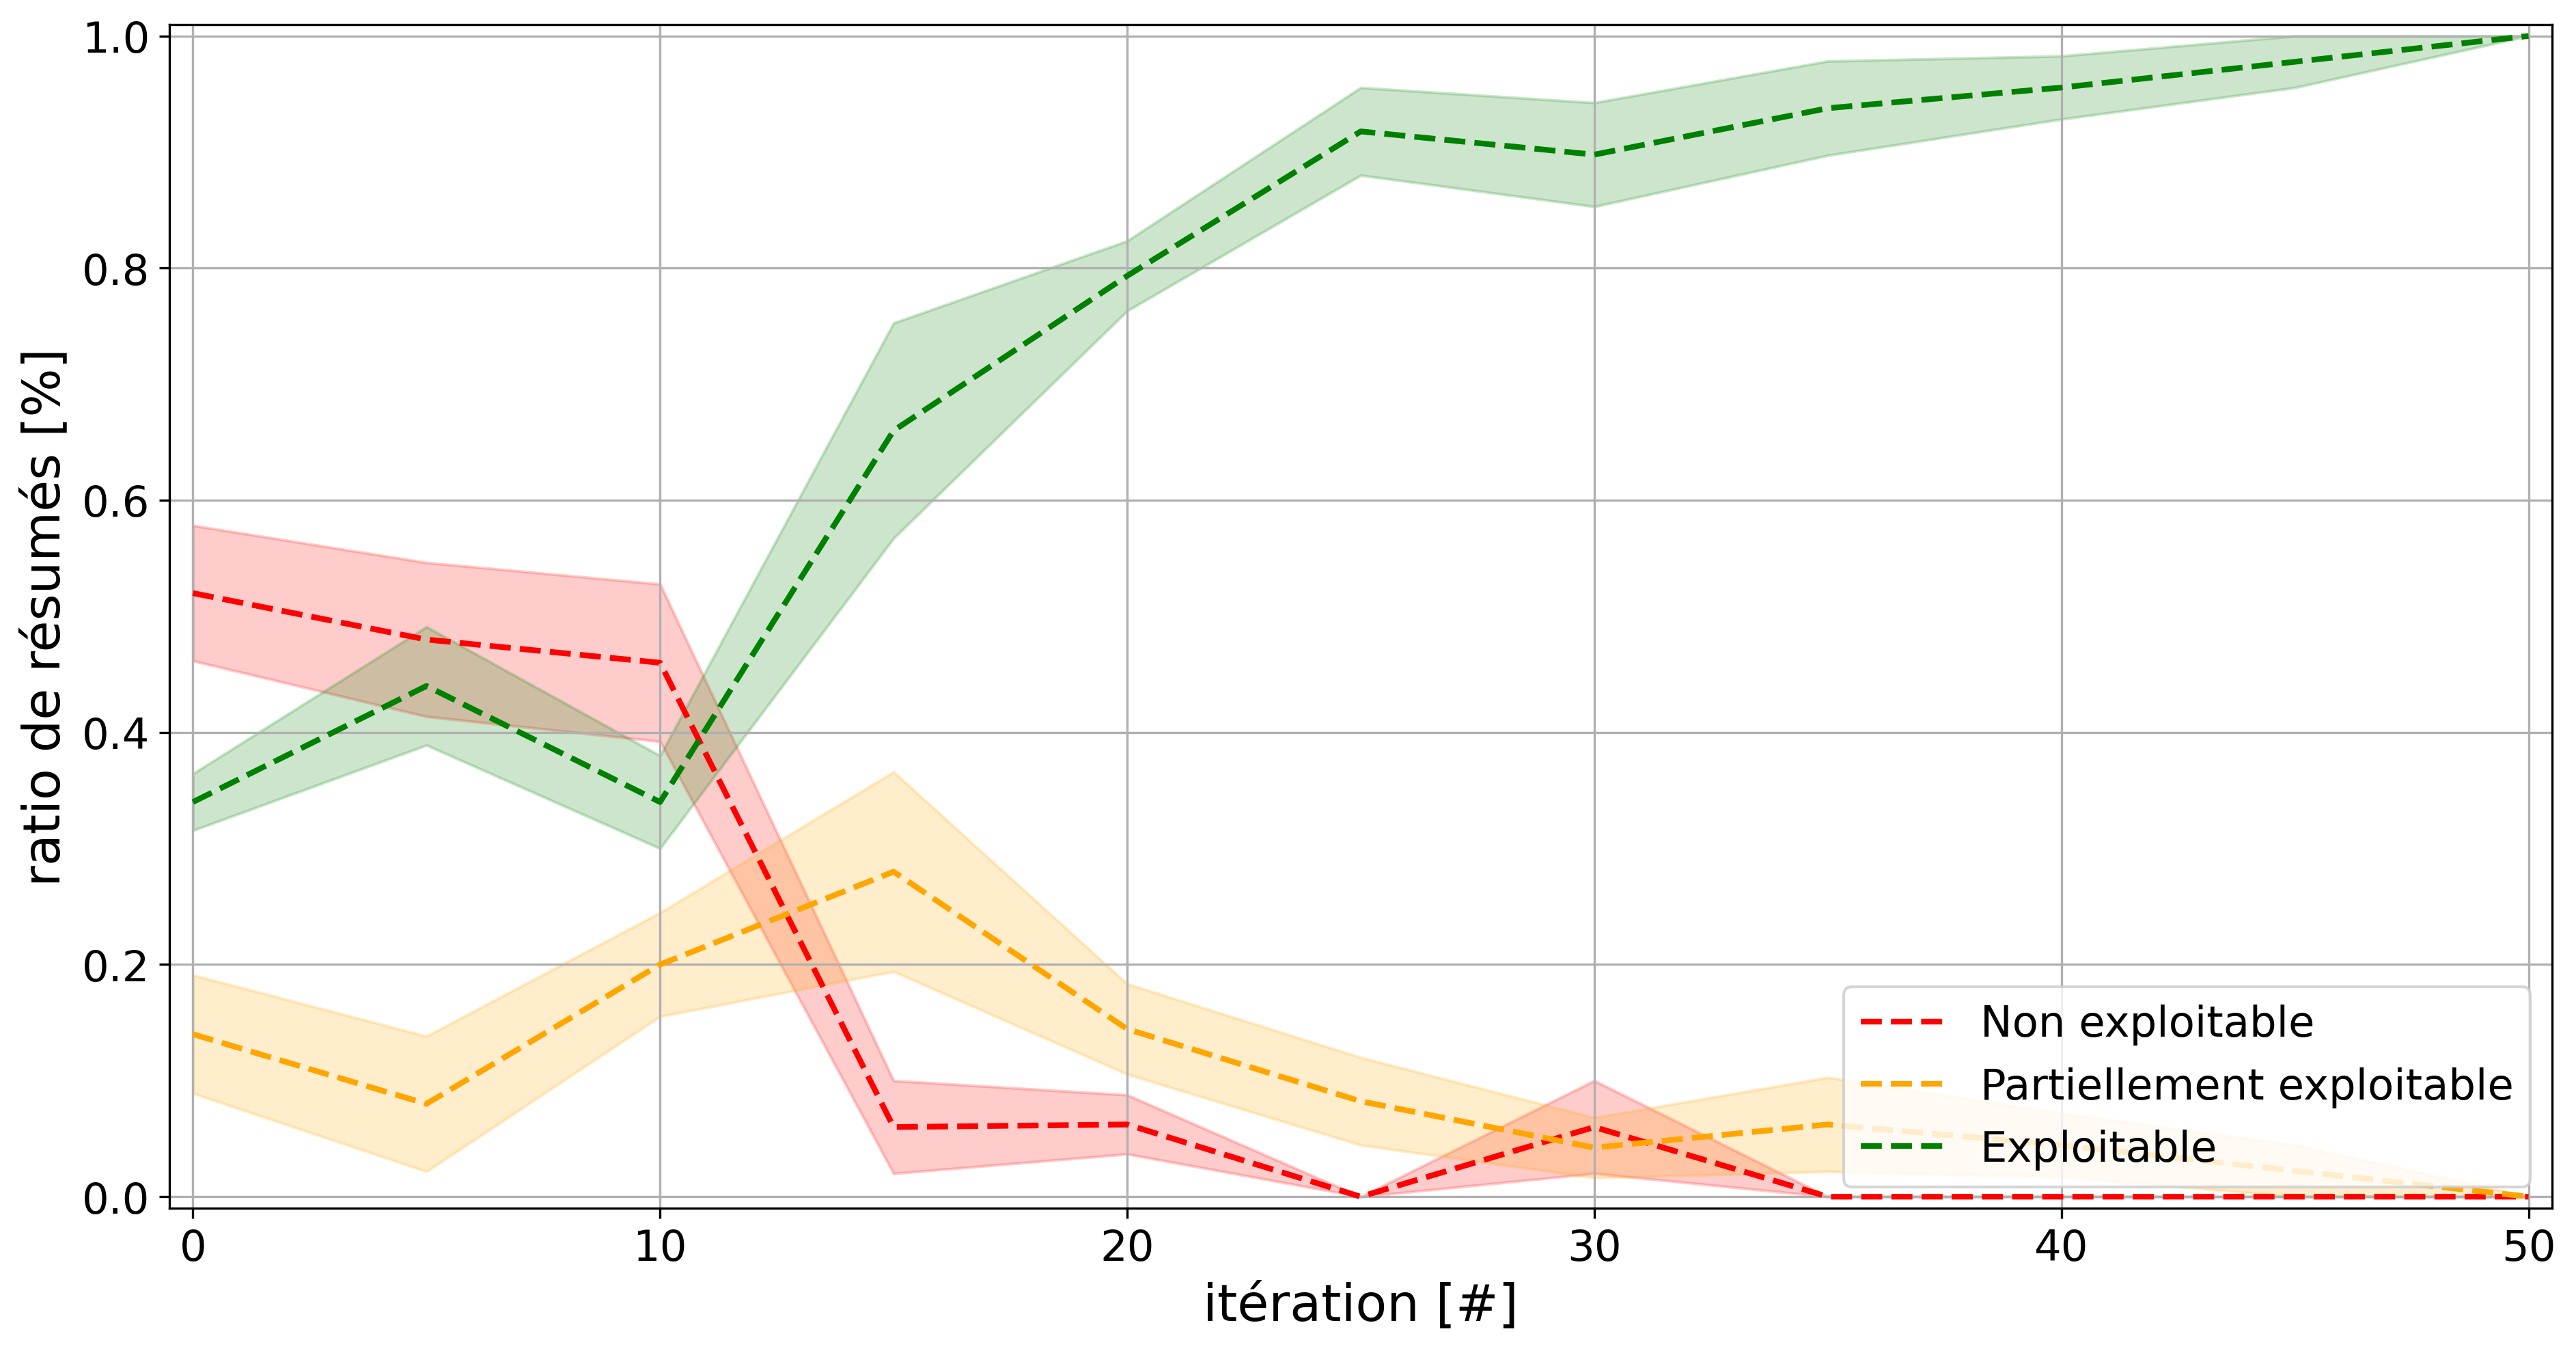
\includegraphics[width=0.95\textwidth]{figures/etude-pertinence-llm-check-resume-annotation-favori}
				\caption{Évolution de la pertinence métier moyenne en fonction du nombre d'itérations de la méthode.
				Cette pertinence, exprimée en proportion du nombre de \textit{clusters}, est estimée sur la base du résumé automatique des \textit{clusters} par un modèle de langue et est retranscrite en trois niveaux : \texttt{exploitable} en vert, \texttt{partiellement exploitable} en orange, et \texttt{non exploitable} en rouge.}
				\label{figure:4.4.3-ETUDE-PERTINENCE-RESUME-AUTOMATIQUE}
			\end{figure}
			
			% Description de deux cas d'études.
			Pour aller plus loin, reprenons les \textit{clusters} que nous avons utilisé comme cas d'étude lors de l'analyse linguistique à l'aide de la maximisation des traits (cf. \textsc{Section~\ref{section:4.4.2-ETUDE-PERTINENCE-PATTERNS-LINGUISTIQUES}}).
			
			% Exemple d'un cluster qui est bien formé dès le début.
			D'abord, reprenons l'exemple de l'évolution d'un \textit{cluster} bien formé dès l'itération $0$, précédemment détaillé dans la \textsc{Table~\ref{table:4.4.2-ETUDE-PERTINENCE-PATTERNS-LINGUISTIQUES-GESTION-SANS-CONTACT}} et dont les résumés automatiques sont présentés dans la \textsc{Table~\ref{table:4.4.3-ETUDE-PERTINENCE-RESUME-AUTOMATIQUE-GESTION-SANS-CONTACT}}.
			Nous constatons effectivement que les synthèses générées par le modèle identifie sans ambiguïté le thème du paiement sans contact, même si le résumé de l'itération $0$ énumère longuement les actions réalisables sur ce sujet.
			
			\todo[inline]{A REDIGER: tableau avec exemples ?}
			
			\begin{table}[!htb]
				\begin{center}
				\def\arraystretch{0.8}  % interligne
				\begin{tabular}{|c|c|}
				
				\hline
				% ENTETE DU TABLEAU
				Identification
					& \multirow{2}{*}{
						Résumé automatique du cluster (\texttt{LLM})
					}
					\tabularnewline
				du cluster
					&
					\tabularnewline
					\hline
				
				% Exemple 1.1:
				{ \footnotesize Tentative: $1$ }
					& \multirow{5}{*}{\parbox{12cm}{
						\footnotesize La thématique traitée dans ces textes est la gestion de l'activation, la désactivation, la modification ou la nécessité d'utiliser le paiement sans contact ou le NFC (Near Field Communication) sur les cartes de paiement bancaires.
					}}
					\tabularnewline
				{ \footnotesize Itération: $0$ }
					&
					\tabularnewline
				{ \footnotesize Cluster: $0$ }
					&
					\tabularnewline
				{ \footnotesize Avis initial: }
					&
					\tabularnewline
				{ \footnotesize \color{colorDarkPastelGreen} \texttt{Exploitable} }
					&
					\tabularnewline
					\hline
					
				% Exemple 1.2:
				{ \footnotesize Tentative: $1$ }
					& \multirow{5}{*}{\parbox{12cm}{
						\footnotesize Les textes traitent de la gestion et de l'utilisation du paiement sans contact (NFC) sur les cartes bancaires.
					}}
					\tabularnewline
				{ \footnotesize Itération: $15$ }
					&
					\tabularnewline
				{ \footnotesize Cluster: $0$ }
					& 
					\tabularnewline
				{ \footnotesize Avis initial: }
					&
					\tabularnewline
				{ \footnotesize \color{colorDarkPastelGreen} \texttt{Exploitable} }
					&
					\tabularnewline
					\hline
					
				\end{tabular}
				\end{center}
				\caption{Extrait de de l'analyse de résumés automatiques de \textit{clusters} exploitables dès la première itération.
				Ces \textit{clusters} représentent la thématique \texttt{gestion\_sans\_contact} entre l'itération $0$ (initialisation) et l'itération $15$ (atteinte de la vérité terrain).
				La seconde colonne expose le résumé obtenu en appelant un large modèle de langage (\texttt{gpt-3.5-turbo}) sur une tâche de résumé.
				}
				\label{table:4.4.3-ETUDE-PERTINENCE-RESUME-AUTOMATIQUE-GESTION-SANS-CONTACT}
			\end{table}
			
			% Exemple d'un cluster qui se forme.
			Ensuite, intéressons nous l'exemple de l'évolution des \textit{clusters} en cours de formations détaillés dans la \textsc{Table~\ref{table:4.4.2-ETUDE-PERTINENCE-PATTERNS-LINGUISTIQUES-GESTION-SANS-CONTACT}} et dont les résumés automatiques sont présentés dans la \textsc{Table~\ref{table:4.4.3-ETUDE-PERTINENCE-RESUME-AUTOMATIQUE-GESTION-SANS-CONTACT}}.
			À l'itération $0$, le résumé proposé est une longue énumération de $9$ thématiques différentes sur la gestion de carte bancaires : puisque le jeu de données entier traite des cartes bancaires, nous identifions clairement ce \textit{cluster} comme non exploitable.
			À l'itération $10$, nous ne distinguons plus que deux sujets principaux : le déblocage de carte, et l'utilisation de numéros de cartes virtuelles, ce qui est en accord avec notre précédente analyse.
			À partir de l'itération $15$, ces deux thématiques se retrouvent bien séparées dans deux \textit{clusters} différents, et chacune est identifiable via le résumé proposé : on note toutefois que si la thématique principale est identifiée, alors l'énumération de détails est plutôt portée sur les actions réalisables avec cette thématique ("\textit{création}", "\textit{activation}", "\textit{suppression}" pour la classe \texttt{gestion\_carte\_virtuelle}).
			
			\begin{table}[!htb]
				\begin{center}
				\def\arraystretch{0.8}  % interligne
				\begin{tabular}{|c|c|}
				
				\hline
				% ENTETE DU TABLEAU
				Identification
					& \multirow{2}{*}{
						Résumé automatique du cluster (avec un \texttt{LLM})
					}
					\tabularnewline
				du cluster
					&
					\tabularnewline
					\hline

				% Exemple 2.1:
				{ \footnotesize Tentative: $1$ }
					& \multirow{5}{*}{\parbox{12cm}{
						\footnotesize La thématique des textes est la gestion des cartes bancaires, incluant la sécurité, les pertes, les vols, les blocages, les récupérations, le changement ou la commande de cartes, les garanties et assurances, les découverts, les paiements virtuels, les numéros virtuels et les plafonds de paiement autorisés.
					}}
					\tabularnewline
				{ \footnotesize Itération: $0$ }
					&
					\tabularnewline
				{ \footnotesize Cluster: $1$ }
					&
					\tabularnewline
				{ \footnotesize Avis initial: }
					&
					\tabularnewline
				{ \footnotesize \color{colorDarkPastelRed} \texttt{Non exploitable} }
					&
					\tabularnewline
					\hline
					
				% Exemple 2.2:
				{ \footnotesize Tentative: $1$ }
					& \multirow{6}{*}{\parbox{12cm}{
						\footnotesize Les textes traitent principalement de la gestion des cartes de paiement, de leur déblocage ou leur réactivation, et de l'utilisation de numéros de carte virtuelle pour les achats en ligne.
					}}
					\tabularnewline
				{ \footnotesize Itération: $10$ }
					&
					\tabularnewline
				{ \footnotesize Cluster: $2$ }
					&
					\tabularnewline
				{ \footnotesize Avis initial: }
					&
					\tabularnewline
				{ \footnotesize \color{colorCadmiumOrange} \texttt{Partiellement} }
					&
					\tabularnewline
				{ \footnotesize \color{colorCadmiumOrange} \texttt{exploitable} }
					&
					\tabularnewline
					\hline
					
				% Exemple 2.3a:
				{ \footnotesize Tentative: $1$ }
					& \multirow{5}{*}{\parbox{12cm}{
						\footnotesize Les textes concernent la gestion et l'utilisation des numéros de carte virtuelle pour les achats en ligne, notamment la création, l'activation, la suppression et la gestion de ces numéros virtuels.
					}}
					\tabularnewline
				{ \footnotesize Itération: $15$ }
					&
					\tabularnewline
				{ \footnotesize Cluster: $2$ }
					&
					\tabularnewline
				{ \footnotesize Avis initial: }
					&
					\tabularnewline
				{ \footnotesize \color{colorDarkPastelGreen} \texttt{Exploitable} }
					&
					\tabularnewline
					\hline
					
				% Exemple 2.3b:
				{ \footnotesize Tentative: $1$ }
					& \multirow{5}{*}{\parbox{12cm}{
						\footnotesize La thématique traitée dans ces textes est le déblocage, le déverrouillage ou la réactivation de cartes bancaires bloquées.
					}}
					\tabularnewline
				{ \footnotesize Itération: $15$ }
					&
					\tabularnewline
				{ \footnotesize Cluster: $4$ }
					&
					\tabularnewline
				{ \footnotesize Avis initial: }
					&
					\tabularnewline
				{ \footnotesize \color{colorDarkPastelGreen} \texttt{Exploitable} }
					&
					\tabularnewline
					\hline
					
				\end{tabular}
				\end{center}
				\caption{Extrait de de l'analyse de résumés automatiques de \textit{clusters} évoluant de non exploitables à exploitables.
				Ces \textit{clusters} représentent la conception des thématiques \texttt{gestion\_carte\_virtuelle} et \texttt{deblocage\_carte}, entre l'itération $0$ (initialisation) et l'itération $15$ (atteinte de la vérité terrain).
				La seconde colonne expose le résumé obtenu en appelant un large modèle de langage (\texttt{gpt-3.5-turbo}) sur une tâche de résumé.
				}
				\label{table:4.4.3-ETUDE-PERTINENCE-RESUME-AUTOMATIQUE-DEBLOCAGE-CARTE-GESTION-CARTE-VIRTUELLE}
			\end{table}
			
			% Présence de quelques cas abhérants.
			De manière plus globale, en considérant les $376$ \textit{clusters} évalués lors des itérations n'ayant pas encore atteint la vérité terrain\footnote{Nous n'incluons pas les itérations ayant atteint la vérité terrain car les \textit{clusters} sont alors stables et cohérents, donc le modèle n'a aucun obstacle pour générer un résumé sans ambiguïté ni hallucination.}, les résumés automatiques permettent d'identifier les mêmes thématiques qu'une vérification manuelle dans $85$\% des cas ($312$ \textit{clusters}).
			Concernant les $15$\% de différences, nous avons différents cas de figure :
			\begin{itemize}
				\item si le modèle génère un résumé concis, certaines thématiques peuvent être ignorées : 
				\item à l'inverse, les données aberrantes ou isolées d'un \textit{cluster} peuvent influencer le résumé, donnant l'illusion que plusieurs thématiques sont présentes alors qu'une seule ne l'est réellement ;
				\item le résumé issu du large modèle de langage peut aussi identifier des thématiques auquel l'expert n'aurait pas pensé : c'est le cas dans les \textit{clusters} $7$ et $8$ de la tentative $1$ à l'itération $0$, où les thématiques \texttt{gestion\_carte\_mastercard} et \texttt{gestion\_carte\_visa} sont proposées dans la synthèse, mais n'aurait pas été par un expert (il n'y a pas de différences aussi significatives entre les deux réseaux de cartes bancaires pour justifier une gestion séparée) ;
				\item enfin, le modèle peut aussi générer des hallucinations n'ayant rien à voir avec les données en entrée : c'est le cas avec le cluster $9$ de la tentative $2$ à l'itération $10$, où le cluster est composé de $2$ questions (« \textit{Comment obtenir une Mastercard ?} » et « \textit{Désactiver les numéros virtuels.} ») et où le résumé parle de "\textit{sécurisation des transactions bancaires}"
			\end{itemize}

		%%% Discussion
		\subsubsection{Discussion}
			\todo[inline]{A REDIGER}
		
			% Remaques expérience utilisateur.
			\todo[inline]{A REDIGER: C'est super pratique, super accessible}
			\todo[inline]{A REDIGER: C'est parfois un peu ambigu...}
			
			% Conclusions et suggestion.
	
	
	%%%
	%%% Subsection 4.4.4: Étude de la cohérence statistique de la base d'apprentissage en cours de construction
	%%%
	%\subsection{Étude de la cohérence statistique de la base d'apprentissage en cours de construction}
	%\label{section:4.4.4-ETUDE-PERTINENCE-COHERENCE}
	%	
	%	% Objectif de l'expérience.
	%	\todo[inline]{A REDIGER: objectif de l'expérience}
	%
	%	%%% Protocole expérimental.
	%	\subsubsection{Protocole expérimental}
	%		\todo[inline]{A REDIGER}
	%		% Axiome.
	%		% Pseudo-code.
	%		% Détails de l'expérience.
	%		% Référence scripts.
	%
	%	%%% Résultats
	%	\subsubsection{Résultats obtenus}
	%		\todo[inline]{A REDIGER}
	%	
	%		% Description statistiques.
	%		
	%		% Exemple.
	%		
	%		% Figure.
	%		%
	%		\begin{figure}[!htb]
	%			\centering
	%			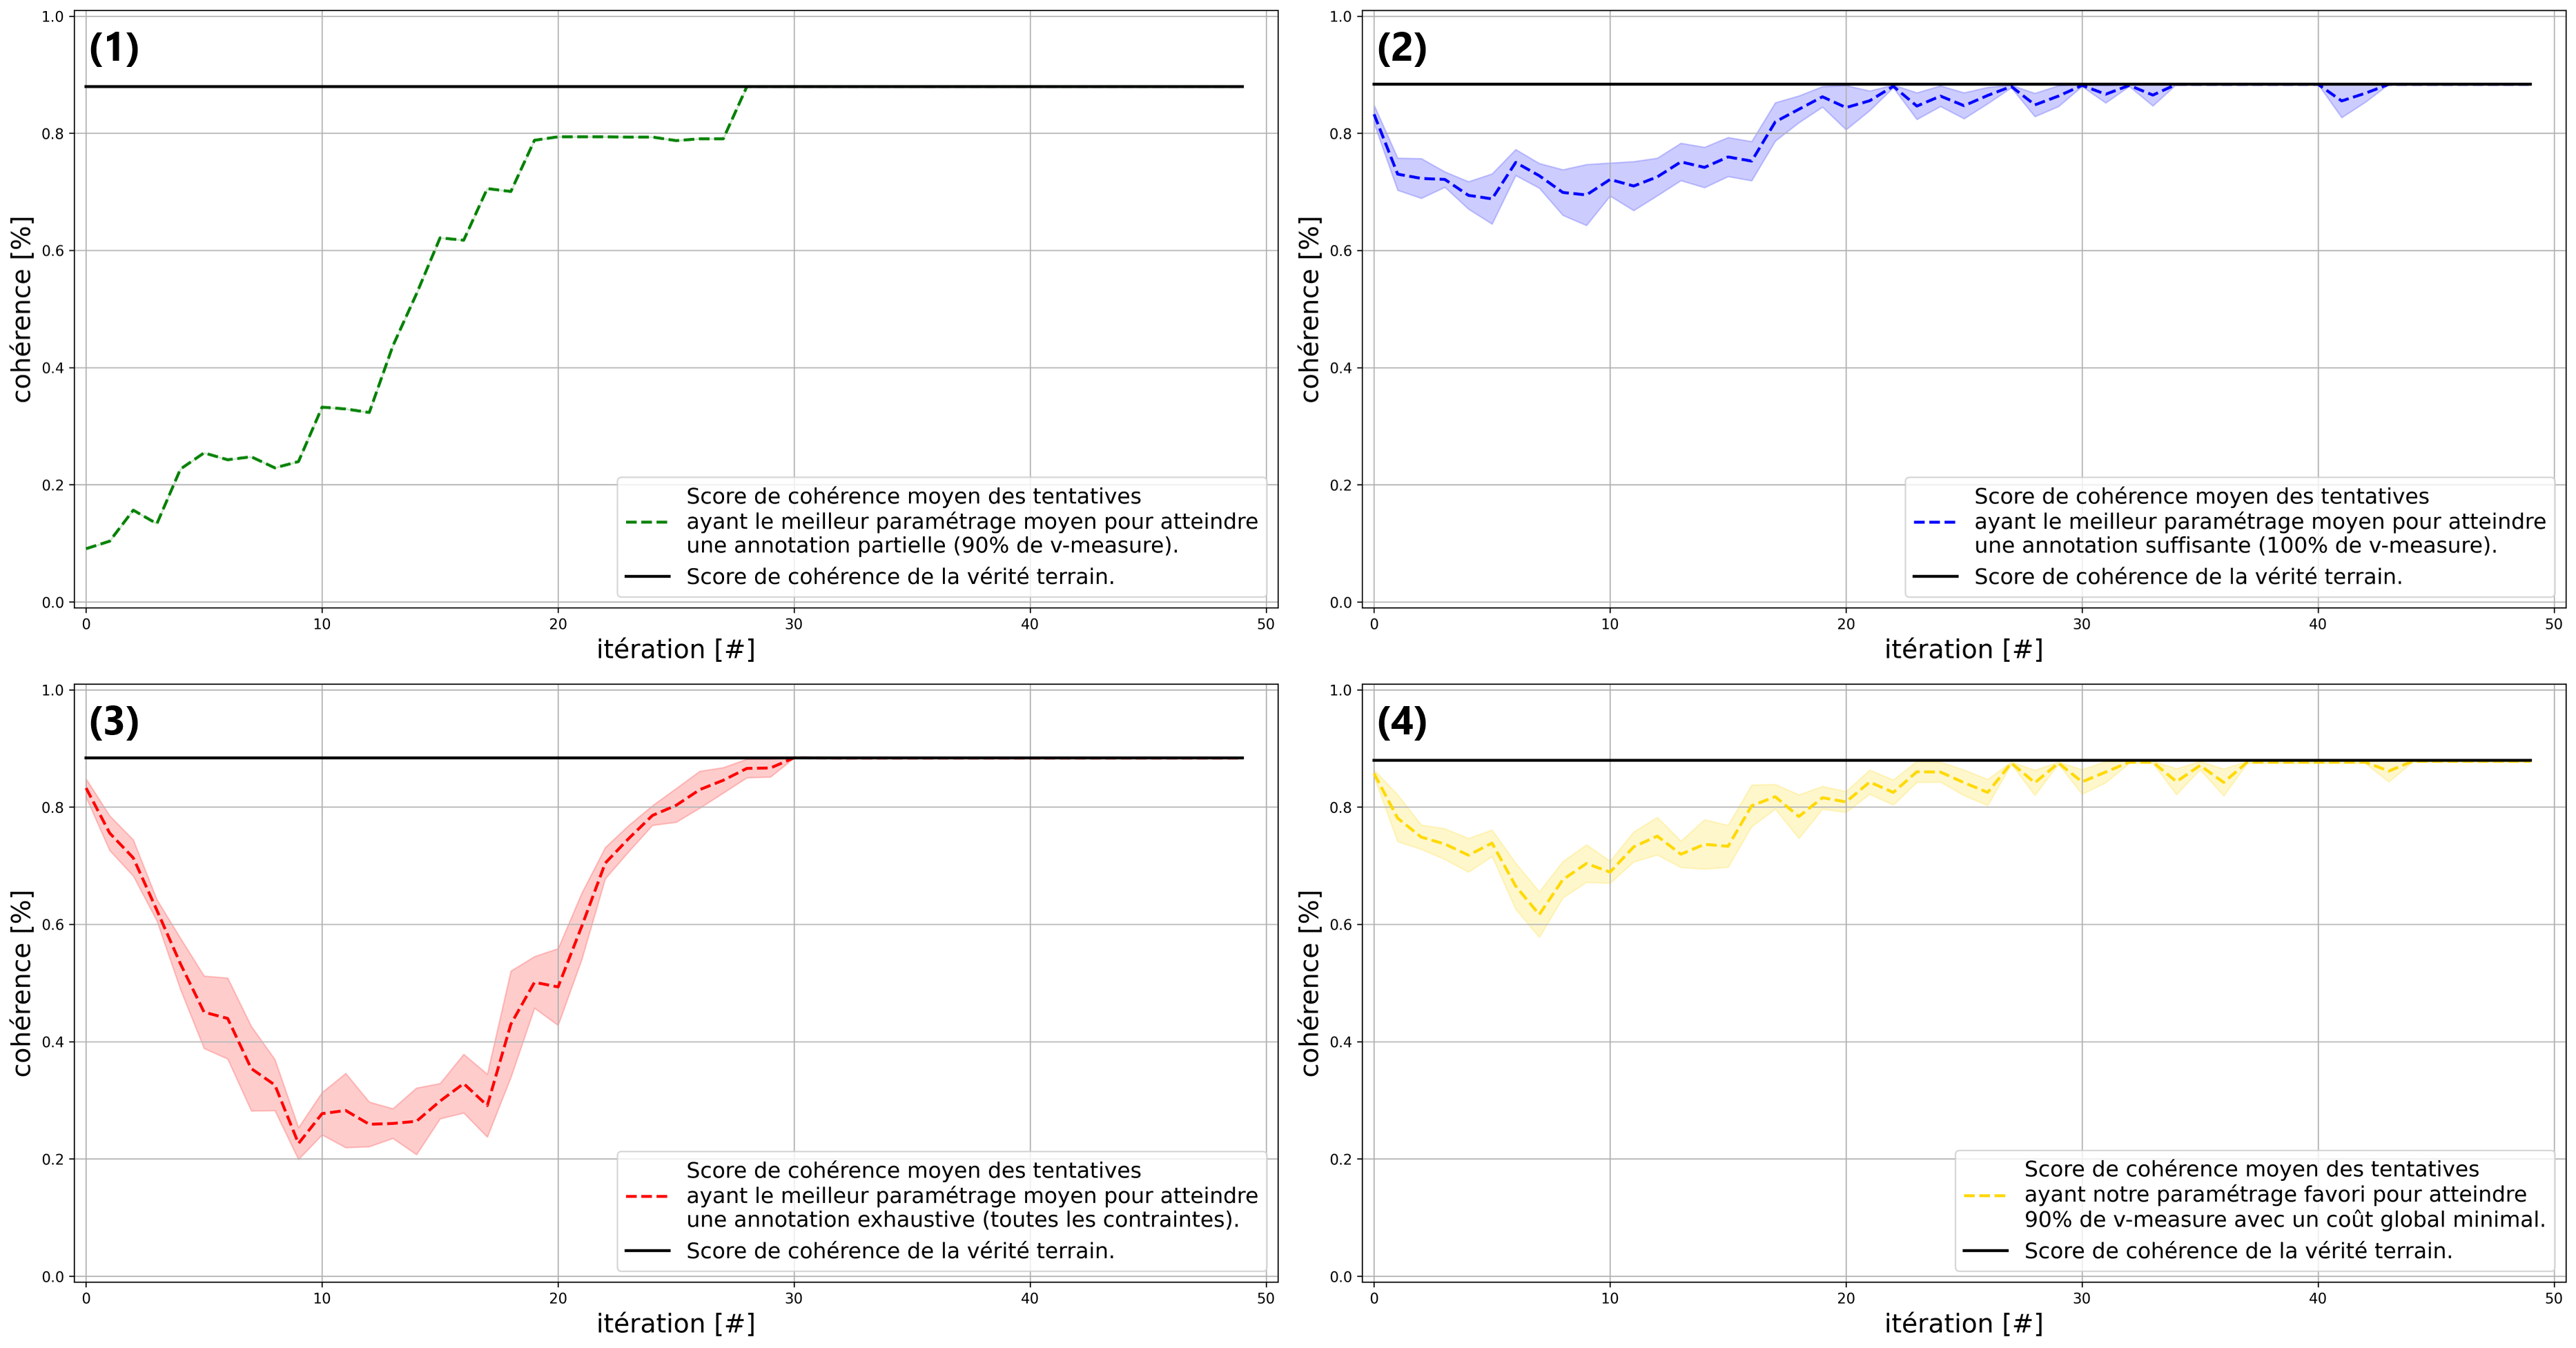
\includegraphics[width=0.95\textwidth]{figures/etude-pertinence-consistence}
	%			\caption{Évolution du score de cohérence moyen des tentatives en fonction de leur paramétrage : \textbf{(1)} meilleur paramétrage moyen une annotation partielle (\texttt{90}\% de \texttt{v-measure}), \textbf{(2)} meilleur paramétrage moyen une annotation suffisante (\texttt{100}\% de \texttt{v-measure}), \textbf{(3)} meilleur paramétrage moyen une annotation exhaustive (annoter toutes les contraintes possibles), et \textbf{(4)} paramétrage favori (\texttt{90}\% de \texttt{v-measure} avec un coût minimal). \\
	%			Note : \textit{Le score de cohérence de la vérité terrain peut varier en fonction des méthodes de prétraitements et de vectorisation utilisées.}}
	%			\label{figure:4.4.4-ETUDE-PERTINENCE-COHERENCE-ANNOTATION}
	%		\end{figure}
	%
	%	%%% Discussion
	%	\subsubsection{Discussion}
	%		\todo[inline]{A REDIGER}
	%	
	%		% Remaques expérience utilisateur.
	%		
	%		% Conclusions et suggestion.
	
	
	%%%%%--------------------------------------------------------------------
	%%%%% Section 4.5: Hypothèse de rentabilité.
	%%%%%--------------------------------------------------------------------
	\newpage
	\section{Évaluation de l'hypothèse de rentabilité}
\label{section:4.5-HYPOTHESE-RENTABILITE}

	%%%
	%%% Introduction / Transition.
	%%%
	Dans les études précédentes, le cas d'arrêt de notre méthodologie d'annotation basée sur le \texttt{Clustering Interactif} était conditionné à la vérité terrain.
	En effet, nous utilisions un seuil de $90$\% de \texttt{v-measure}, caractérisant une annotation dite "partielle" de la base d'apprentissage.
	Cependant, une telle référence n'est pas accessible en situation réelle car l'objectif de notre méthode est précisément de construire cette vérité terrain.
	Nous devons donc nous intéresser à d'autres moyens pour estimer la rentabilité d'une itération supplémentaire, et pouvoir ainsi définir de nouveaux cas d'arrêt pour le \texttt{Clustering Interactif}.
	Pour cela, nous aimerions vérifier l'hypothèse suivante :
	
	%%%
	%%% Formulation des hypothèses.
	%%%
	\begin{tcolorbox}[
		title=\faVial~\textbf{Hypothèse de rentabilité}~\faVial,
		colback=colorTcolorboxHypothesis!15,
		colframe=colorTcolorboxHypothesis!75,
		width=\linewidth
	]
		\textguillemets{\textbf{
			Au cours d'une méthodologie d'annotation basée sur le \texttt{Clustering Interactif}, il est possible d'estimer la rentabilité d'une itération supplémentaire de la méthode, et ainsi d'établir des cas d'arrêt indépendants d'une vérité terrain pour obtenir une base d'apprentissage satisfaisante.
		}} \\
		
		% Figure.
		La \textsc{Figure~\ref{figure:4.5-HYPOTHESE-RENTABILITE}} illustre cette hypothèse et la perspective de pouvoir estimer le rapport entre le gain de pertinence obtenu et le coût nécessaire pour l'obtenir.
		%
		\begin{figure}[H]  % keep [H] to be in the tcolorbox.
			\centering
			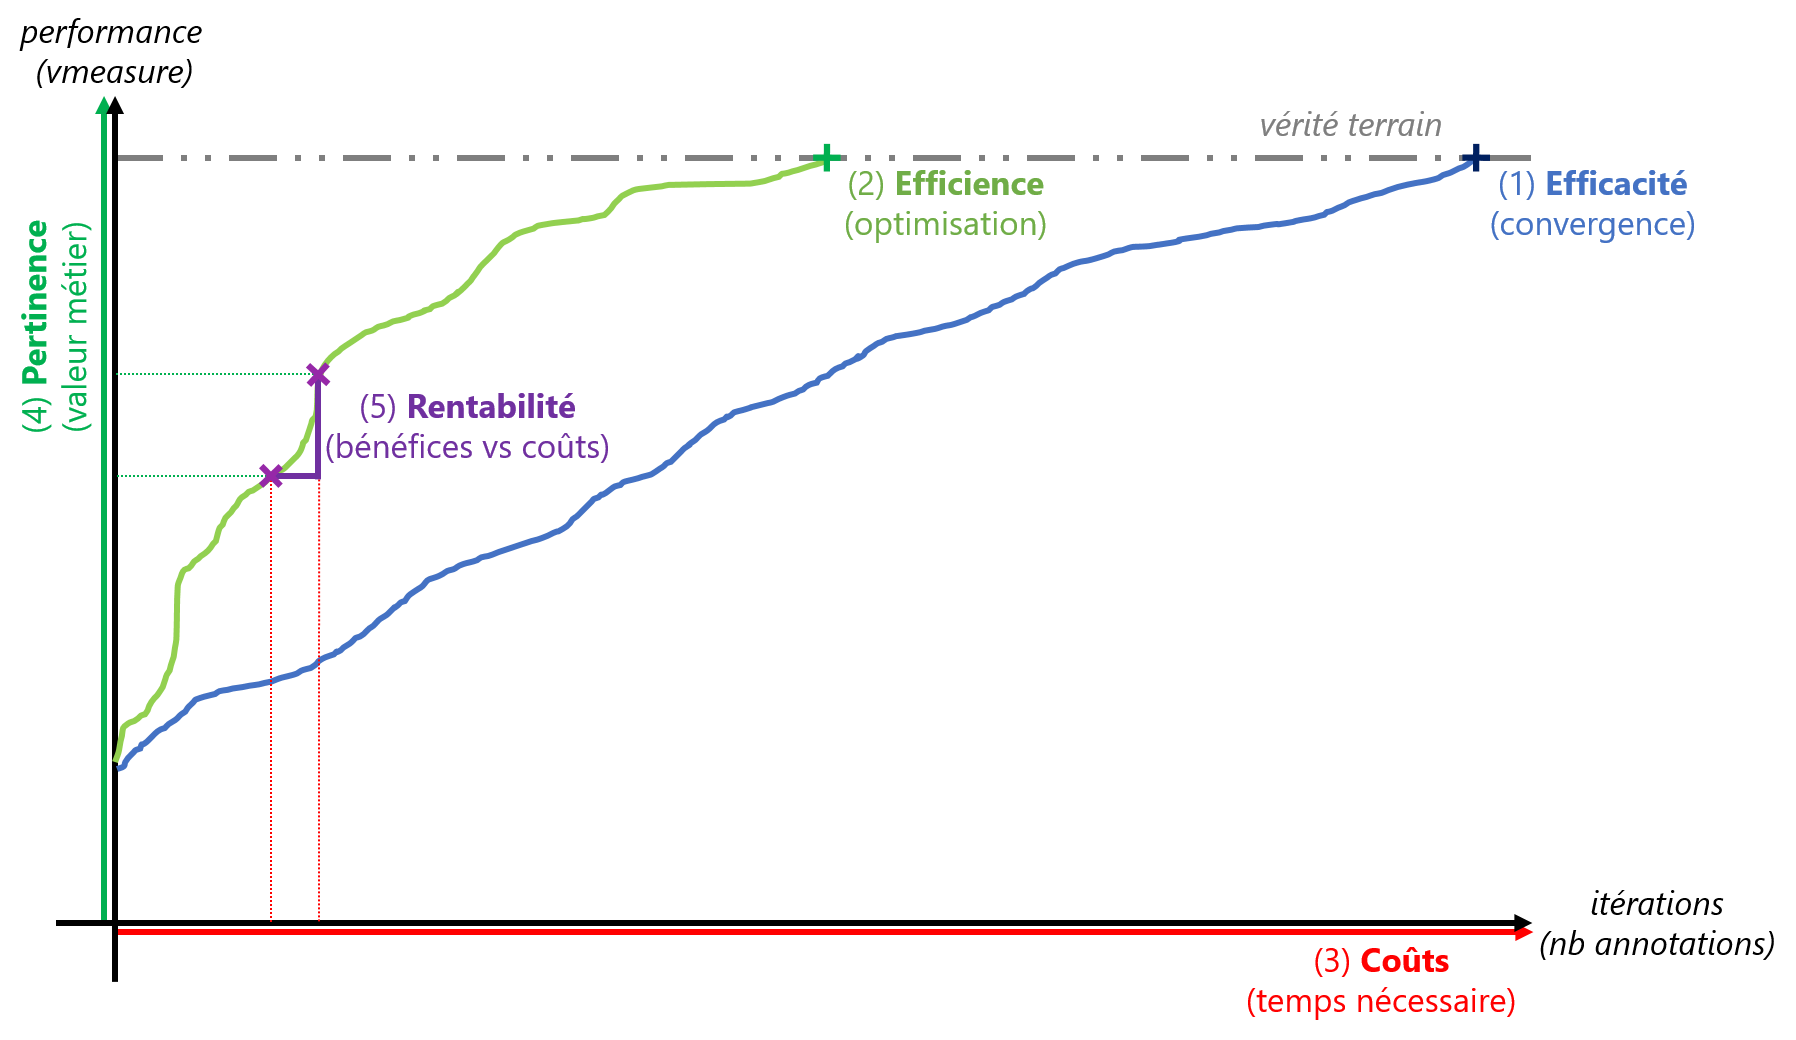
\includegraphics[width=0.95\textwidth]{figures/hypotheses-05-rentabilite}
			\caption{
				Illustration des études réalisées sur le \texttt{Clustering Interactif} (\textit{étape 5/6}) en schématisant l'évolution de la \textbf{pertinence} (\textit{valeur métier évaluée par l'expert, exprimée en nombre de clusters}) d'une base d'apprentissage en cours de construction, en fonction du coût temporel de la méthode (\textit{temps nécessaire à l'expert métier et à la machine}), ainsi que la \textbf{rentabilité} de chaque itération de la méthode (\textit{rapport entre le gain potentiel de pertinence et le coût à investir}).
			}
			\label{figure:4.5-HYPOTHESE-RENTABILITE}
		\end{figure}
	\end{tcolorbox}
		
	% Résumé des études.
	Afin de vérifier cette hypothèse, nous explorons deux approches :
	\begin{itemize}
		\item l'évolution de l'\textbf{accord entre l'annotation de l'expert et le \textit{clustering}} sur lequel est basé l'échantillon d'annotation, permettant d'estimer si la machine doit encore être corrigée par l'annotateur  (cf. \textsc{Section~\ref{section:4.5.1-ETUDE-RENTABILITE-ACCORD-ANNOTATION-CLUSTERING}}) ; et
		\item l'évolution de la \textbf{différence entre deux \textit{clustering} successifs}, permettant de mesurer s'il y a eu des changements visibles dans le partitionnement des données après l'ajout des dernières contraintes (cf. \textsc{Section~\ref{section:4.5.2-ETUDE-RENTABILITE-SIMILARITE-CLUSTERING}}).
	\end{itemize}
	
	
	%%%
	%%% Subsection 4.5.1: Étude de l'évolution d'accord entre l'annotation et le \textit{clustering}.
	%%%
	\subsection{Étude de l'évolution d'accord entre l'annotation et le \textit{clustering}}
	\label{section:4.5.1-ETUDE-RENTABILITE-ACCORD-ANNOTATION-CLUSTERING}
		
		% Objectif de l'expérience.
		Nous cherchons à trouver un cas d'arrêt du \texttt{Clustering Interactif} ne nécessitant pas de comparaison avec une vérité terrain, et notre première intuition concerne l'étude des annotations réalisées.
		En effet, à chaque itération, l'expert annote un échantillon de contraintes dans le but de confirmer ou de corriger le \textit{clustering} de l'itération précédente.
		Or, après un nombre suffisant d'itérations, le \textit{clustering} commence à se stabiliser : il devrait donc y avoir davantage d'annotations qui confirment le \textit{clustering} que d'annotations qui le corrigent, puis n'avoir que des accords entre les annotations et le \textit{clustering}.
		Ainsi, nous allons étudier l'évolution du nombre de contraintes annotées qui approuvent le partitionnement des données obtenu, et essayer d'adapter cette analyse en cas d'arrêt pour notre méthode d'annotation.
	
		%%% Protocole expérimental.
		\subsubsection{Protocole expérimental}
			
			% Axiome.
			\begin{leftBarWarning}
				Dans le cadre de cette étude, nous supposons que l'expert métier connaît parfaitement le domaine traité dans ce jeu de données, et qu'il est capable de caractériser sans ambiguïté la similitude entre deux données issues de cet ensemble.
			\end{leftBarWarning}
			
			% Pseudo-code.
			Pour résumer le protocole expérimental que nous détaillons ci-dessous, une description en pseudo-code est disponible dans l'\textsc{Algorithme~\ref{algorithm:4.5.1-ETUDE-RENTABILITE-ACCORD-ANNOTATION-CLUSTERING-PROTOCOLE}}.
			
			\begin{algorithm}
				\KwData{jeux de données annotées (vérités terrains)}
				%
				\ForEach{jeu de données à tester}{
					\textbf{initialisation (données)}: récupérer les données et la vérité terrain \;
					\textbf{initialisation (contraintes)}: créer une liste vide de contraintes \;
					\textbf{prétraitements}: supprimer le bruit dans les données avec \texttt{prep.simple} \;
					\textbf{vectorisation}: transformer les données en vecteurs avec \texttt{vect.tfidf} \;
					\textbf{clustering initial}: regrouper les données par similarité avec \texttt{clust.kmeans.cop} \;
					\Repeat{annotation de toutes les contraintes possibles}{
						\textbf{échantillonnage}: sélectionner des contraintes avec \texttt{samp.closest.diff} \;
						\textbf{simulation d'annotation}: déterminer les contraintes avec la vérité terrain \;
						\textbf{intégration}: ajouter les nouvelles contraintes au gestionnaire de contraintes \;
						\textbf{rentabilité}: calculer l'accord entre l'annotation et le \textit{clustering} précédent \;
						\textbf{clustering}: regrouper les données par similarité avec \texttt{clust.kmeans.cop} \;
					}
				}
				\textbf{analyse 1}: afficher l'évolution de l'accord entre annotation et \textit{clustering} \;
				\textbf{analyse 2}: calculer la corrélation entre le score d'accord et le score de performance \;
				%
				\KwResult{discussion sur la rentabilité d'après l'accord entre annotation et \textit{clustering}}
				%
				\caption{\textit{
					Description en pseudo-code du protocole expérimental de l'étude de l'évolution d'accord entre l'annotation et le \textit{clustering}.
				}}
				\label{algorithm:4.5.1-ETUDE-RENTABILITE-ACCORD-ANNOTATION-CLUSTERING-PROTOCOLE}
			\end{algorithm}
			
			% Description de la vérité terrain.
			Nous utilisons comme vérité terrain le jeu de données \texttt{Bank Cards (v1.0.0)} : ce dernier traite des demandes les plus fréquentes des clients en ce qui concerne la gestion de leur carte bancaire.
			Il est composé de $500$ questions rédigées en français et réparties en $10$ classes (\texttt{perte ou vol de carte}, \texttt{carte avalée}, \texttt{commande de carte}, ...).
			Pour plus de détails, consulter l'\textsc{Annexe~\ref{annex:A.1-DATASET-BANK-CARDS}}.
			
			% Description des tentatives de la méthode et du calcul de rentabilité.
			Sur ce jeu de données, nous exécutons une tentative complète \footnote{
				Tentative complète : itérations d'échantillonnage, d'annotation et de \textit{clustering} jusqu'à annotation de toutes les contraintes possibles.
			}
			de la méthode du \texttt{Clustering Interactif} en utilisant notre paramétrage favori \footnote{
				Paramétrage favori (atteindre $90$\% de \texttt{v-measure} avec un coût minimal): prétraitements simples (\texttt{prep.simple}), vectorisation \texttt{TF-IDF} (\texttt{vect.tfidf}), \textit{clustering} \texttt{KMeans} avec modèle \texttt{COP} (\texttt{clust.kmeans.cop}) et échantillonnage des données les plus proches dans des \textit{clusters} différents (\texttt{sampl.closest.diff}).
			} (voir \textsc{Section~\ref{section:4.3-HYPOTHESE-COUTS}}), et cette tentative est répétée $5$ fois pour contrer les aléas statistiques des exécutions.
			À chaque itération, un lot de $50$ contraintes est sélectionné puis annotés en simulant l'action d'un expert métier, et nous évaluons l'accord entre ces nouvelles annotations et la proposition de partitionnement des données, partitionnement réalisé par le \textit{clustering} à l'itération précédente :
			\begin{itemize}
				\item il y a \textbf{accord} lorsqu'une contrainte de deux données issues d'un même \textit{cluster} est annotée \texttt{MUST-LINK}, ou lorsqu'une contrainte de deux données issues de deux \textit{clusters} différents est annotée \texttt{CANNOT-LINK} (cf. \textsc{Figure~\ref{figure:4.5.1-ETUDE-RENTABILITE-ACCORD-ANNOTATION-CLUSTERING-EXEMPLE} (1)}) ;
				\item il y a \textbf{désaccord} lorsqu'une contrainte de deux données issues d'un même \textit{cluster} est annotée \texttt{CANNOT-LINK}, ou lorsqu'une contrainte de deux données issues de deux \textit{clusters} différents est annotée \texttt{MUST-LINK} (cf. \textsc{Figure~\ref{figure:4.5.1-ETUDE-RENTABILITE-ACCORD-ANNOTATION-CLUSTERING-EXEMPLE} (2)}).
			\end{itemize}
			Nous pouvons ainsi calculer un score d'accord défini par le ratio entre le nombre d'accords et le nombre de contraintes annotées.
			Pour nous permettre de discuter de l'utilité de ce score pour prédire la stabilisation du \textit{clustering} et ainsi définir un cas d'arrêt de notre méthodologie d'annotation, nous calculons aussi le score de corrélation entre cet accord et la performance obtenue à l'aide d'une vérité terrain (la corrélation \texttt{r} de \textit{Pearson} (\cite{kirch:2008:pearson-correlation-coefficient}) est utilisée).

			\begin{figure}[!htb]
				\centering
				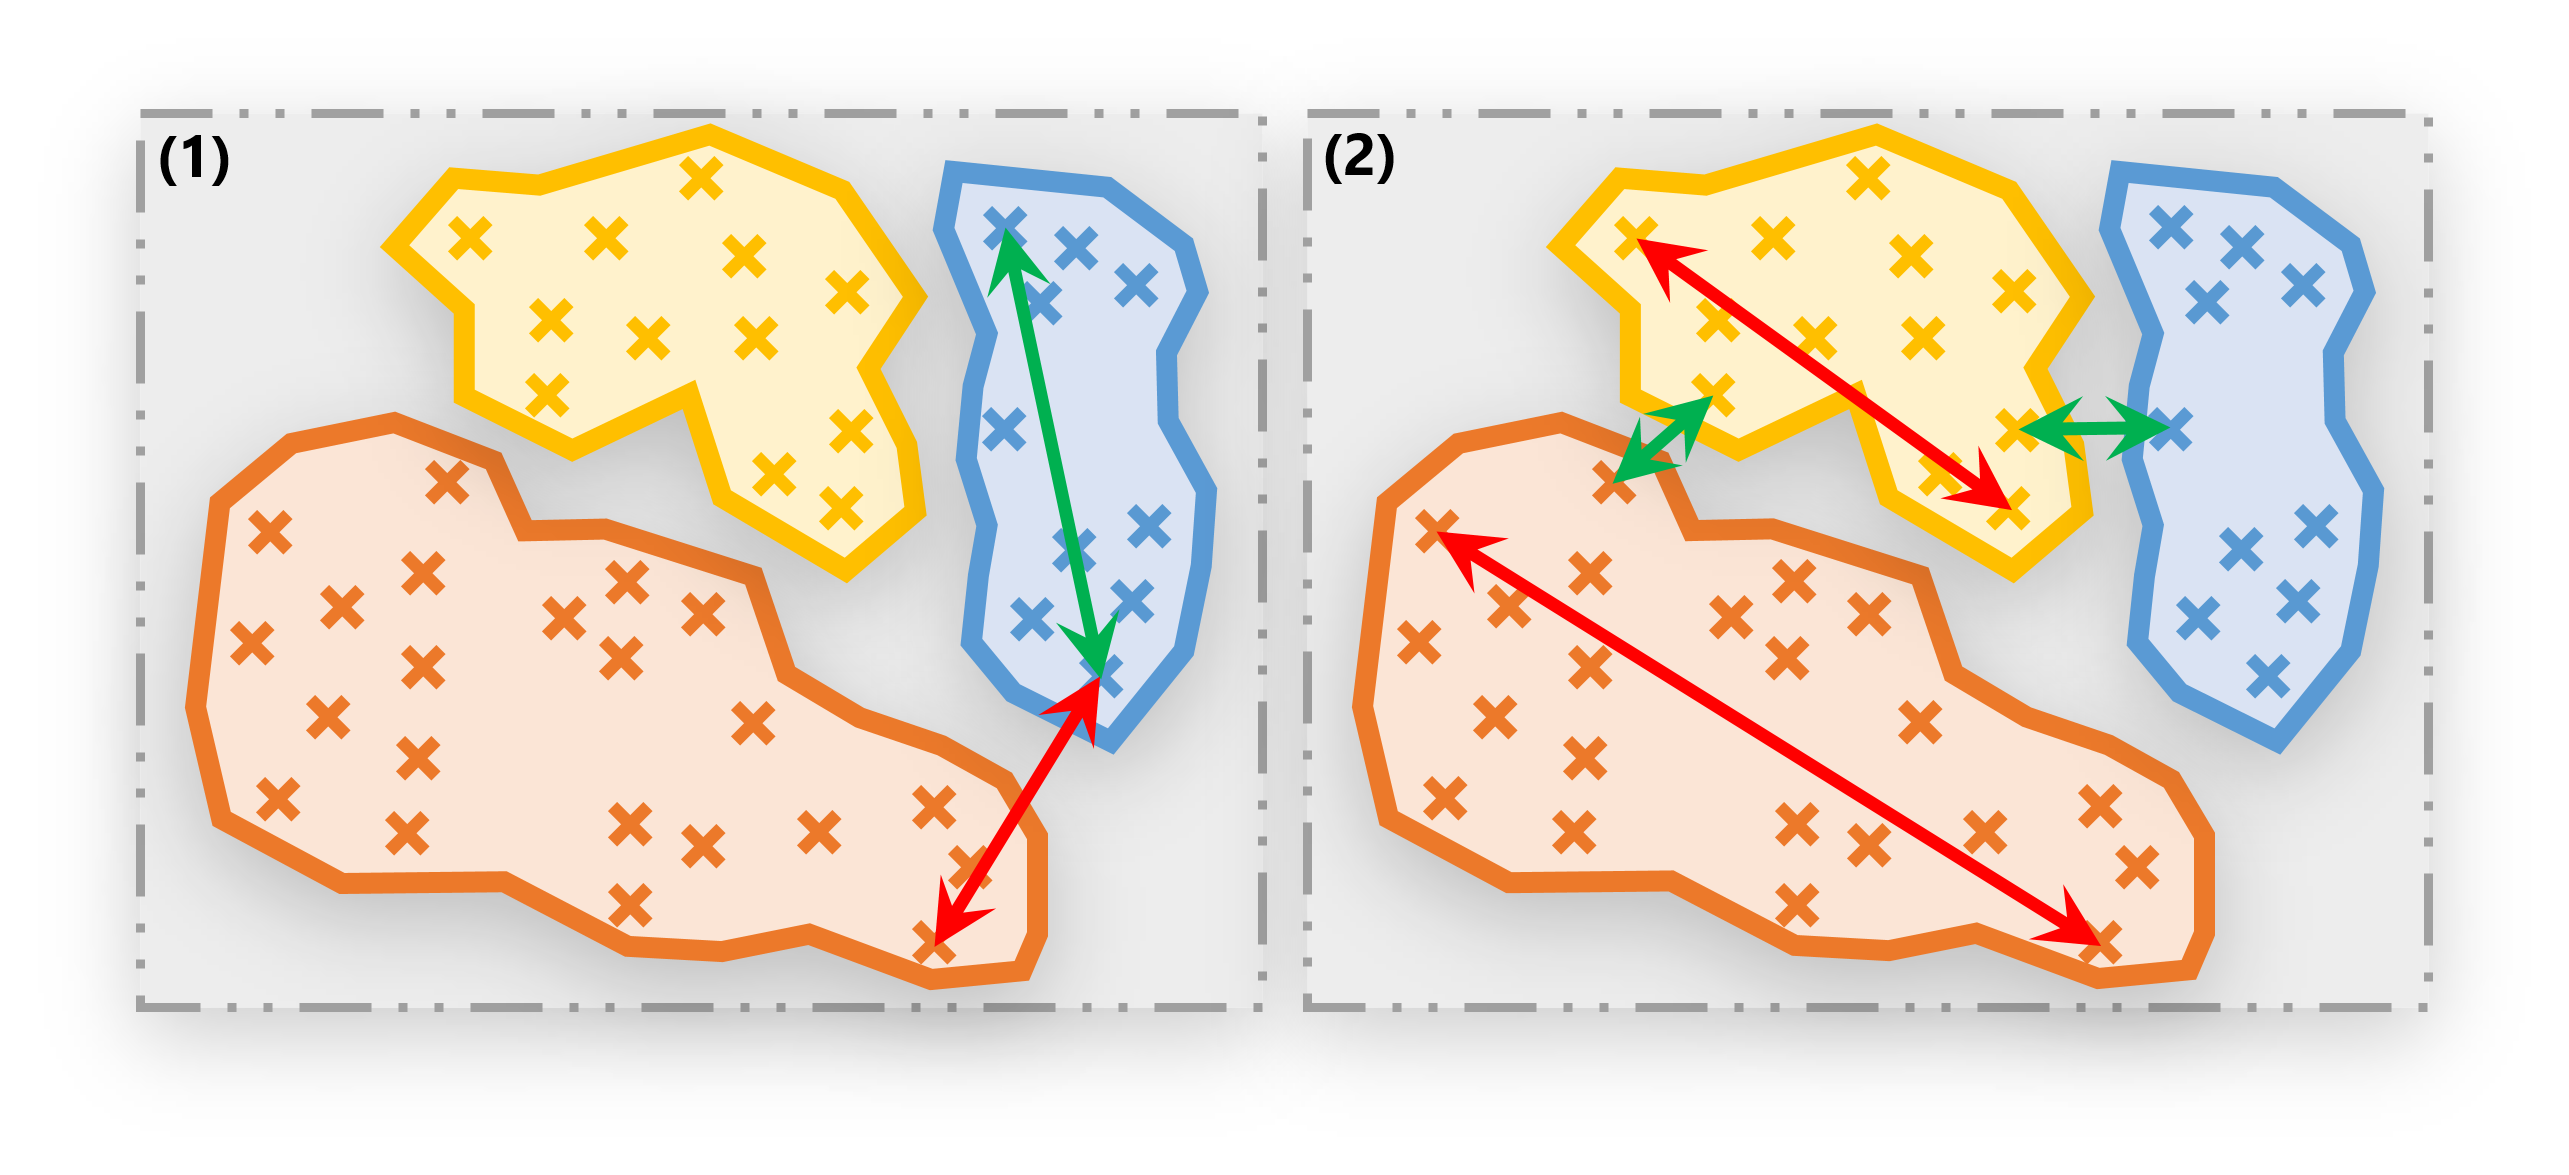
\includegraphics[width=0.70\textwidth]{figures/example-accord-annotation-clustering}
				\caption{
					Exemples d'accords et de désaccords entre les annotations d'une itération et le résultat du \textit{clustering} de l'itération précédente.
					Des contraintes \texttt{MUST-LINK} (flèches vertes) et \texttt{CANNOT-LINK} (flèches rouges) sont représentées dans deux situations : \textbf{(1)} montre des cas d'accords (\texttt{MUST-LINK} dans un même \textit{cluster}, \texttt{CANNOT-LINK} entre deux \textit{clusters} différents), et \textbf{(2)} montre des cas de désaccords (\texttt{MUST-LINK} entre deux \textit{clusters} différents, \texttt{CANNOT-LINK} dans un même \textit{cluster}).
				}
				\label{figure:4.5.1-ETUDE-RENTABILITE-ACCORD-ANNOTATION-CLUSTERING-EXEMPLE}
			\end{figure}
			
			\begin{leftBarIdea}
				Nous concentrons l'étude sur notre paramétrage favori (voir \textsc{Section~\ref{section:4.4.3-ETUDE-PERTINENCE-RESUME-AUTOMATIQUE}}).
				Cependant, afin de compléter notre discussion avec d'autres points de comparaison, nous analysons aussi les autres paramétrages implémentés, notamment les meilleurs paramétrages moyens identifiés lors de l'hypothèse d'efficience (voir \textsc{Section~\ref{section:4.2-HYPOTHESE-EFFICIENCE}}).
			\end{leftBarIdea}
			
			% Référence scripts.
			\begin{leftBarInformation}
				Les scripts de l'expérience, réalisés avec des \textit{notebooks} \texttt{Python} (\cite{van-rossum-drake:2009:python-reference-manual}), sont disponibles dans un dossier dédié de \cite{schild:2021:cognitivefactory-interactiveclusteringcomparativestudy}.
				De plus, les jeux de données ainsi que les implémentations de notre \texttt{Clustering Interactif} sont détaillés respectivement en \textsc{Annexe~\ref{annex:A-ANNEXE-DATASET}} et en \textsc{Annexe~\ref{annex:C-ANNEXE-IMPLEMENTATIONS}}.
			\end{leftBarInformation}

		%%% Résultats
		\subsubsection{Résultats obtenus}
			
			% Figure : croissance générale.
			La \textsc{Figure~\ref{figure:4.5.1-ETUDE-RENTABILITE-ACCORD-ANNOTATION-CLUSTERING}} représente l'évolution moyenne du score d'accord entre annotation et \textit{clustering} pour les quatre paramétrages mis en avant lors de nos études.
			Nous pouvons constater une tendance générale à la croissance de ce score d'accord : pour le paramétrage favori \textbf{(4)}, l'accord est plutôt faible au début de la méthode (inférieur à $45$\% avant l'itération $15$), puis devient de plus en plus fort (dépassant les $60$\%) pour finalement atteindre les $100$\% vers l'itération $45$.
			\begin{figure}[!htb]
				\centering
				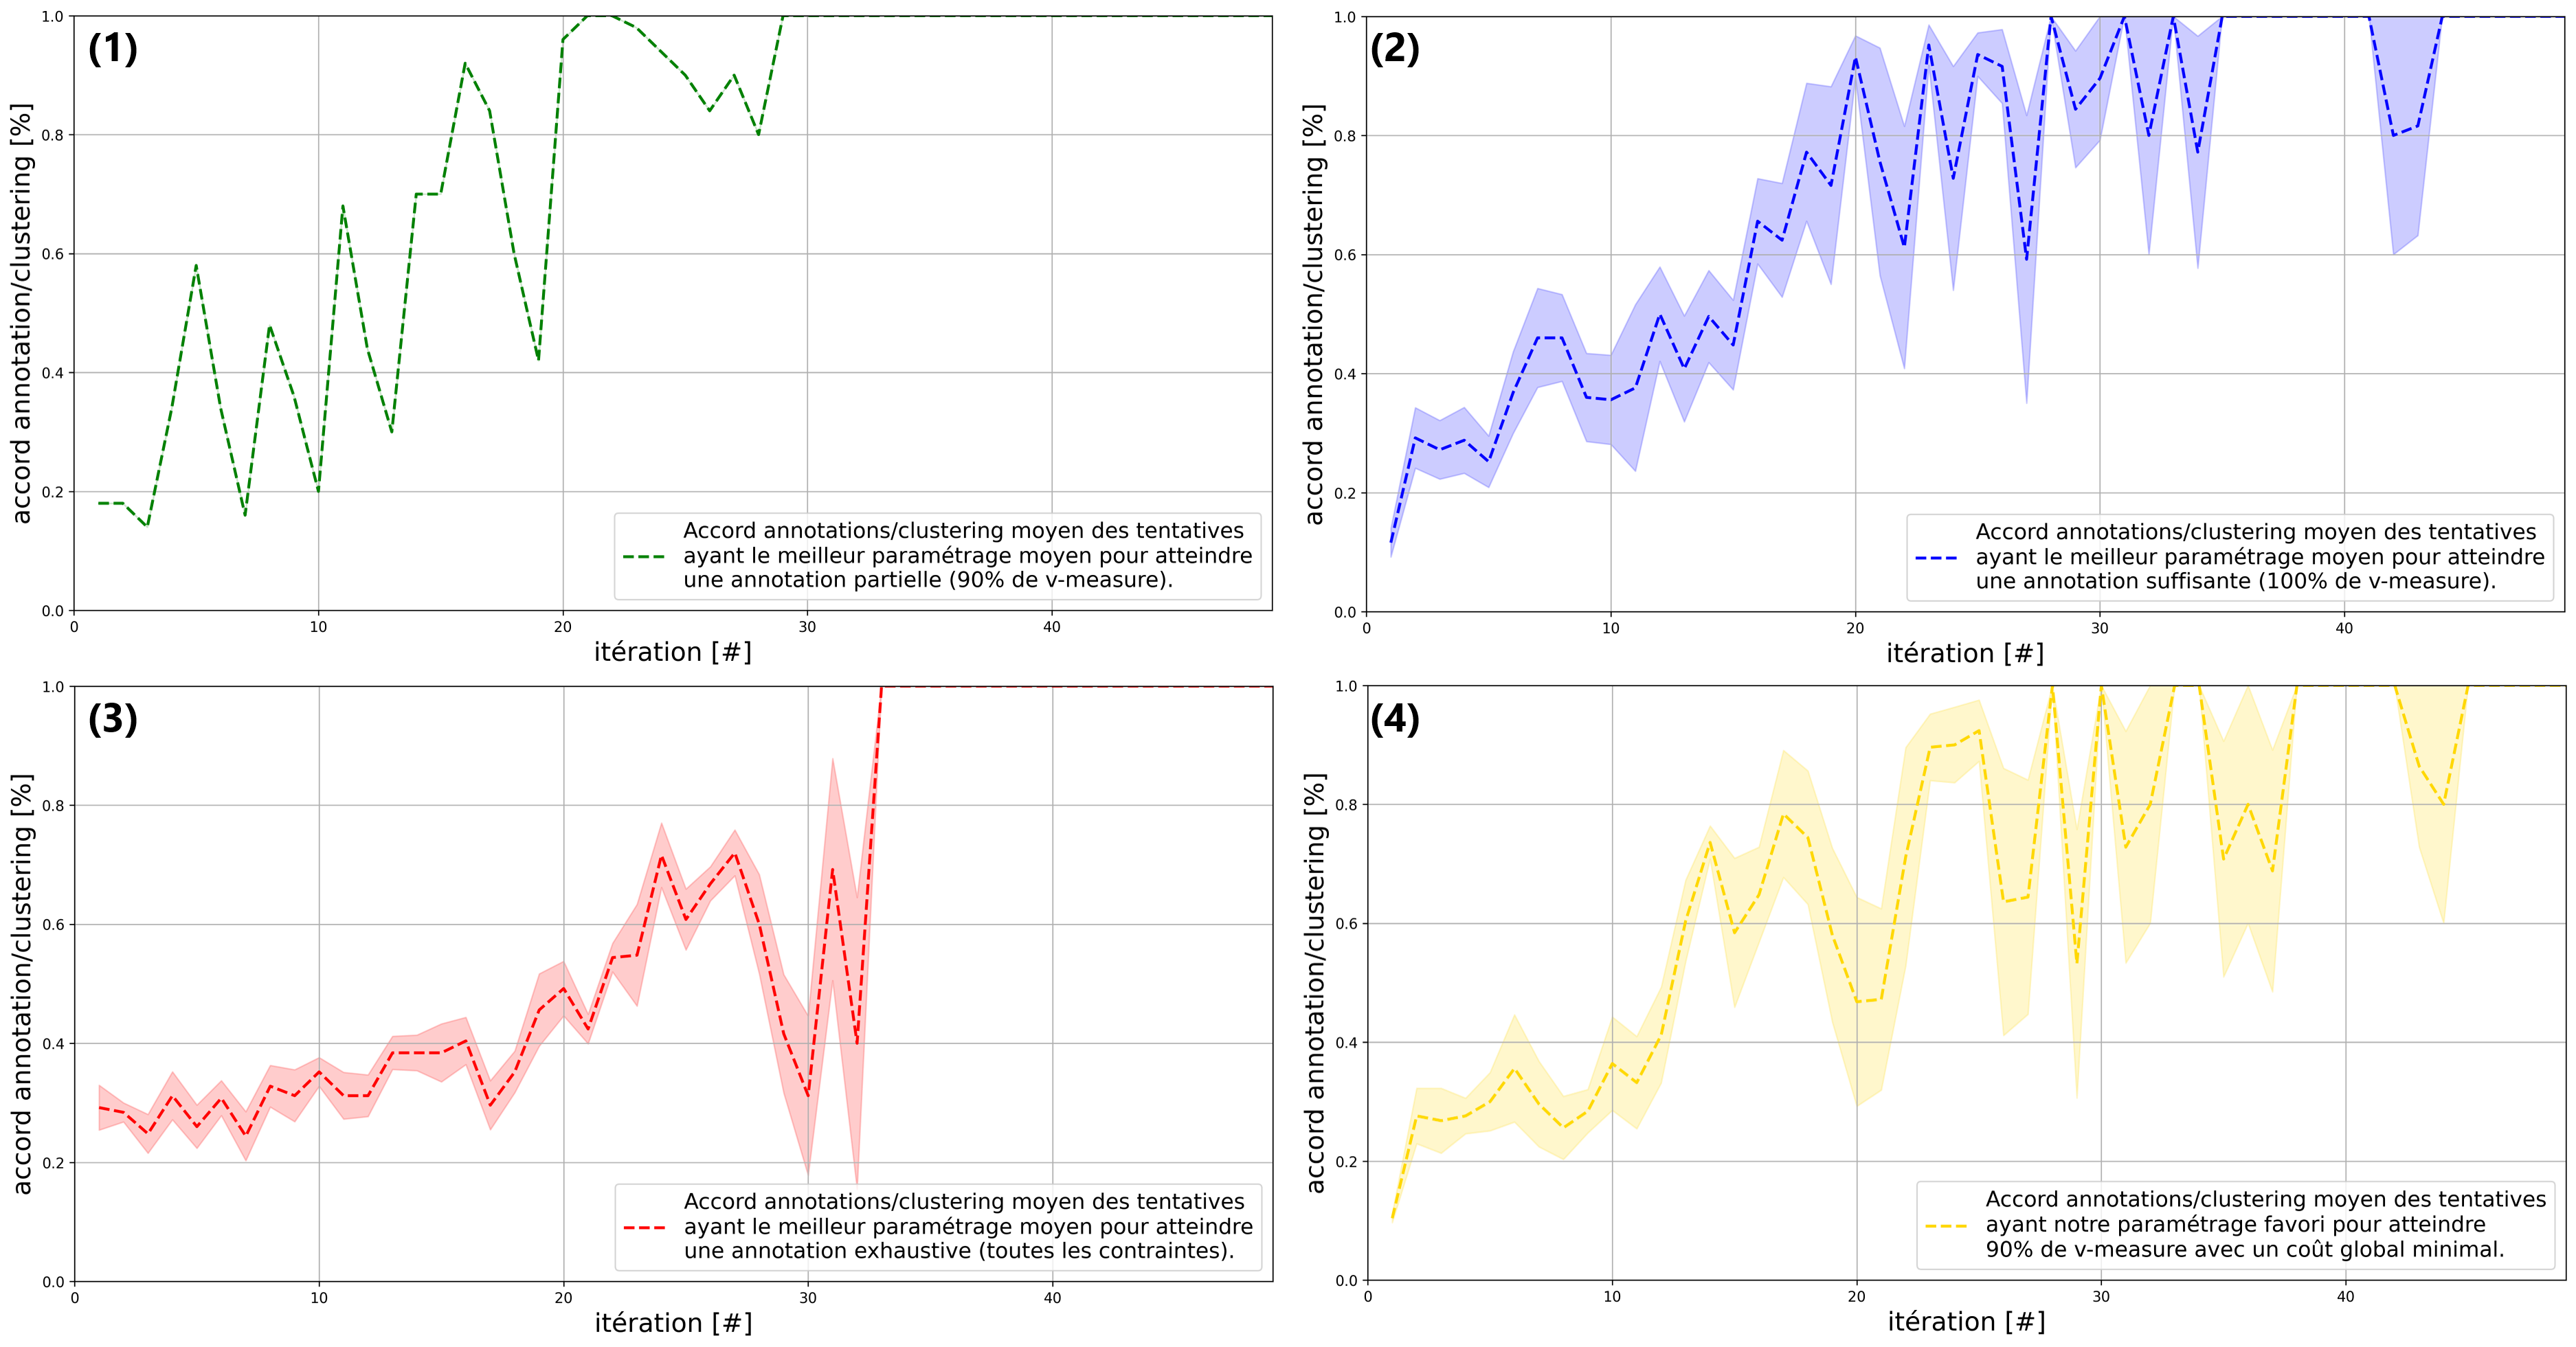
\includegraphics[width=0.95\textwidth]{figures/etude-rentabilite-accord-annotation}
				\caption{
					Évolution au cours des itérations de l'accord entre l'annotation de contraintes d'un expert et le résultat de \textit{clustering} sur lequel est basé l'échantillonnage de contraintes.
					Ces accords sont exprimés grâce à des lots de $50$ contraintes annotées.
					Les évolutions moyennes de différents paramétrages de la méthode sont exposées :
					\textbf{(1)} meilleur paramétrage moyen pour atteindre une annotation partielle ;
					\textbf{(2)} meilleur paramétrage moyen pour atteindre une annotation suffisante ;
					\textbf{(3)} meilleur paramétrage moyen pour atteindre une annotation exhaustive ;
					et \textbf{(4)} paramétrage favori.
					À titre d'information, les courbes en noir représentent l'évolution de la \texttt{v-measure} entre le \textit{clustering} et la vérité terrain.
				} 
				\label{figure:4.5.1-ETUDE-RENTABILITE-ACCORD-ANNOTATION-CLUSTERING}
			\end{figure}
			
			% Tableau : corrélation modérée.
			La \textsc{Table~\ref{table:4.5.1-ETUDE-RENTABILITE-CORRELATION-ACCORD-PERFORMANCE}} contient le score de corrélation entre cet accord et la performance théoriques obtenue grâce à la vérité terrain.
			Cette corrélation est modérée : $0.49$ sur l'ensemble des tentatives, $0.69$ sur les tentatives utilisant notre paramétrage favori.
			%
			\begin{table}[!htb]
				\begin{center}
				\begin{tabular}{|c|r|}
				
					\hline
					% ENTETE DU TABLEAU
					\rowcolor{colorTableHeader!15}
					\multicolumn{1}{|c|}{\shortstack[c]{
						Paramétrage
					}}
						& \multicolumn{1}{c|}{\shortstack[c]{
							Corrélation \texttt{r}
						}}
						\tabularnewline
						\hline \hline
					
					% Annotation partielle.
					Meilleur paramétrage moyen pour une annotation partielle \textbf{(1)}
						& $0.92$
						\tabularnewline
						\hline
					
					% Annotation suffisante.
					Meilleur paramétrage moyen pour une annotation suffisante \textbf{(2)}
						& $0.74$
						\tabularnewline
						\hline
					
					% Annotation exhaustive.
					Meilleur paramétrage moyen pour une annotation exhaustive \textbf{(3)}
						& $0.57$
						\tabularnewline
						\hline
					
					% Paramétrage favori
					Paramétrage favori \textbf{(4)}
						& $0.69$
						\tabularnewline
						\hline
					
					% Moyenne des $960$ tentatives.
					Moyenne des $960$ tentatives
						& $0.49$
						\tabularnewline
						\hline
					
				\end{tabular}
				\end{center}
				\caption{
					Score de corrélation \texttt{r} de \textit{Pearson} entre la performance du \textit{clustering} obtenu à l'aide d'une vérité terrain (\texttt{v-measure}) et le score d'accord entre annotation et \textit{clustering}.
				}
				\label{table:4.5.1-ETUDE-RENTABILITE-CORRELATION-ACCORD-PERFORMANCE}
			\end{table}
			
			% Description de la figure : croissance instable.
			Cependant, la tendance constatée est aussi saccadée par de nombreux pics pouvant faire perdre ou gagner jusqu'à $40$\% d'accord entre deux itérations.
			Des chutes d'accord peuvent intervenir au niveau des itérations où la similarité du \textit{clustering} avec la vérité terrain est pourtant forte, comme c'est le cas autour des itérations $29$ et $36$ où l'accord chute de plus de $25$\% alors que la \texttt{v-measure} avec la vérité terrain est constamment au dessus de de $95$\%.
			
			% Description de la figure : autres paramétrages
			Les autres paramétrages représentés dans \textbf{(1)}, \textbf{(2)} et \textbf{(3)} comportent des tendances similaires (corrélation forte mais variations soudaines d'accord, chute d'accords malgré des \textit{clustering} aux performances élevées, ...).

		%%% Discussion
		\subsubsection{Discussion}
		
			% Rappel de l'objectif : trouver un cas d'arrêt en regardant l'accord entre l'annotation et le \textit{clustering}.
			Dans cette étude, nous avons analysé l'évolution de l'accord entre les annotations et le partitionnement de données proposé par un \textit{clustering} dans l'espoir de définir un cas d'arrêt de notre méthodologie d'annotation qui soit indépendant d'une vérité terrain préétablie.
			Cependant, en considérant les résultats obtenus, ce score d'accord ne semble pas répondre à cet objectif.
			
			% Trop instable pour définir un cas d'arrêt.
			Tout d'abord, malgré une corrélation acceptable avec la performance théorique du \textit{clustering} (moyenne à $0.49$, voir \textsc{Table~\ref{table:4.5.1-ETUDE-RENTABILITE-CORRELATION-ACCORD-PERFORMANCE}}), l'évolution du score d'accord reste instable.
			En effet, les nombreuses variations et saccades rendent toute analyse de rentabilité difficile, voire impossible, ce qui ne permet pas de définir un cas d'arrêt pour notre méthode d'annotation.
			
			\begin{leftBarExamples}
				Concernant l'évolution du paramétrage favori (\textsc{Figure~\ref{figure:4.5.1-ETUDE-RENTABILITE-ACCORD-ANNOTATION-CLUSTERING}} \textbf{(4)}), nous ne pouvons pas précisément définir à partir de quelle itération les résultats semblent intéressants, car le score d'accord oscille longuement entre $50$\% et $100$\% avec des pics de plus de $25$\% entre deux itérations. 
			\end{leftBarExamples}
			
			\begin{leftBarAuthorOpinion}
				% Rappel: l'objectif de notre méthode d'annotation est de corriger le plus rapidement un \textit{clustering}.
				Après réflexion, ce score d'accord est probablement infructueux à cause du fonctionnement même de notre méthode, dont l'objectif est de corriger le partitionnement des données en utilisant un minimum de contraintes.
				En effet, dans le cadre de l'optimisation des paramètres réalisée en \textsc{Section~\ref{section:4.2-HYPOTHESE-EFFICIENCE}}, nous avons retenu dans notre paramétrage favori la sélection des contraintes les plus proches entre deux \textit{clusters} différents (\texttt{samp.closest.diff}) : cette sélection permet ainsi de décrire efficacement l'emplacement des frontières de \textit{clusters}.
				
				% Cet échantillonnage est non supervisé : il y a de nombreuses saccades.
				Or, cet échantillonnage reste une méthode non supervisée : lors des premières itérations, les contraintes sélectionnées ont de bonnes chances de mettre en avant une frontière mal positionnée, mais au fur et à mesure que des contraintes s'ajoutent, les nouvelles contraintes ont moins de chances de trouver des bordures de \textit{clusters} qui ne soient pas encore caractérisées.
				De ce fait, il se peut que les dernières sélections n'identifient aucune nouvelle frontière, qu'elles se concentrent sur des frontières déjà bien positionnées ou déjà décrites par d'autres contraintes, ou qu'elles nécessitent plusieurs itérations pour caractériser des frontières complexes (le comportement des autres méthodes de sélections représentées en \textsc{Figure~\ref{figure:4.5.1-ETUDE-RENTABILITE-ACCORD-ANNOTATION-CLUSTERING}} peut être illustré par des raisonnements similaires).
				L'ensemble de ces cas de figures peut ainsi expliquer les nombreuses saccades dans l'évolution du score d'accord : tantôt la sélection semble pertinente, tantôt la sélection semble inutile.
			\end{leftBarAuthorOpinion}
			
			% Trop instable pour caratériser une itération.
			Pour aller plus loin, nous pouvons aussi critiquer le score de corrélation qui ne semble pas montrer de lien fort entre les performances théoriques et les accords calculés, tant sur l'ensemble des tentatives que pour le paramétrage favori.
			Il est même rare d'observer des chutes importantes d'accords qui soient accompagnées d'une variation significative de \texttt{v-measure} avec la vérité terrain.
			Au final, ce score d'accord n'est donc pas vraiment représentatif de la rentabilité d'une itération ou de l'évolution de la pertinence du \textit{clustering}.
			\begin{leftBarAuthorOpinion}
				Pour expliquer cette absence de corrélation, il est possible que l'analyse des annotations ait été une idée infructueuse : les $50$ contraintes annotées peuvent peut-être exprimer un désaccord avec le précédent \textit{clustering}, mais ce n'est pas pour autant que l'ajout de nouvelles contraintes impacte significativement la pertinence globale du partitionnement des données.
			\end{leftBarAuthorOpinion}
			
			% Conclusions et suggestion.
			En conclusion, \textbf{le score d'accord entre l'annotation courante et le \textit{clustering} précédent n'est pas adéquat pour estimer un cas d'arrêt de notre méthode d'annotation}, principalement car il est trop instable et qu'il ne représente pas bien les bénéfices obtenus à chaque itération.
			Ainsi, comme l'analyse de l'annotation n'est pas fructueuse, nous nous tournons vers l'analyse basée sur les différences entre deux résultats de \textit{clustering}
	
	%%%
	%%% Subsection 4.5.2: Étude de l'évolution de la différence entre deux \textit{clustering} consécutifs.
	%%%
	\subsection{Étude de l'évolution de la différence entre deux \textit{clustering} consécutifs}
	\label{section:4.5.2-ETUDE-RENTABILITE-SIMILARITE-CLUSTERING}
		
		% Objectif de l'expérience.
		Nous venons de conclure que l'analyse de l'accord entre l'annotation et le partitionnement des données ne permet pas d'estimer la rentabilité d'une itération de notre méthode d'annotation.
		Parmi les explications possibles, nous avons mis en cause l'analyse du lot de contraintes annotées : en effet, ce n'est pas parce que l'annotation de contraintes est en désaccord avec le précédent partitionnement des données que les correctifs associés auront un impact significatif sur le prochain partitionnement.
		Ainsi, nous voulons analyser l'évolution de la différence entre deux \textit{clustering} successifs : en effet, si une itération apporte des correctifs ayant un impact, alors il devrait y avoir des différences visibles entre les deux itérations de \textit{clustering}.
	
		%%% Protocole expérimental.
		\subsubsection{Protocole expérimental}
			
			% Axiome.
			\begin{leftBarWarning}
				Dans le cadre de cette étude, nous supposons que l'expert métier connaît parfaitement le domaine traité dans ce jeu de données, et qu'il est capable de caractériser sans ambiguïté la similitude entre deux données issues de cet ensemble.
			\end{leftBarWarning}
			
			% Pseudo-code.
			Pour résumer le protocole expérimental que nous détaillons ci-dessous, une description en pseudo-code est disponible dans l'\textsc{Algorithme~\ref{algorithm:4.5.1-ETUDE-RENTABILITE-SIMILARITE-CLUSTERING-PROTOCOLE}}.
			
			\begin{algorithm}
				\KwData{jeux de données annotées (vérités terrains)}
				%
				\ForEach{jeu de données à tester}{
					\textbf{initialisation (données)}: récupérer les données et la vérité terrain \;
					\textbf{initialisation (contraintes)}: créer une liste vide de contraintes \;
					\textbf{prétraitements}: supprimer le bruit dans les données avec \texttt{prep.simple} \;
					\textbf{vectorisation}: transformer les données en vecteurs avec \texttt{vect.tfidf} \;
					\textbf{clustering initial}: regrouper les données par similarité avec \texttt{clust.kmeans.cop} \;
					\Repeat{annotation de toutes les contraintes possibles}{
						\textbf{échantillonnage}: sélectionner des contraintes avec \texttt{samp.closest.diff} \;
						\textbf{simulation d'annotation}: déterminer les contraintes avec la vérité terrain \;
						\textbf{intégration}: ajouter les nouvelles contraintes au gestionnaire de contraintes \;
						\textbf{clustering}: regrouper les données par similarité avec \texttt{clust.kmeans.cop} \;
						\textbf{rentabilité}: calculer la différence entre les deux précédents \textit{clustering} \;
					}
				}
				\textbf{analyse 1}: afficher l'évolution de la différence entre deux \textit{clustering} consécutifs \;
				\textbf{analyse 2}: calculer la corrélation entre le score de différence et le score de performance \;
				%
				\KwResult{discussion sur la rentabilité d'après la différence entre \textit{clustering}}
				%
				\caption{\textit{
					Description en pseudo-code du protocole expérimental de l'étude de l'évolution de la différence entre deux \textit{clustering} consécutifs.
				}}
				\label{algorithm:4.5.1-ETUDE-RENTABILITE-SIMILARITE-CLUSTERING-PROTOCOLE}
			\end{algorithm}

			% Détails de l'expérience.
			Nous nous appuyons sur le même protocole que l'expérience précédente (cf. \textsc{Section~\ref{section:4.5.1-ETUDE-RENTABILITE-ACCORD-ANNOTATION-CLUSTERING}}) : nous utilisons comme vérité terrain le jeu de données \texttt{Bank Cards (v1.0.0)}, nous réalisons $5$ tentatives complètes de la méthode du \texttt{Clustering Interactif} en utilisant notre paramétrage favori (voir \textsc{Section~\ref{section:4.3-HYPOTHESE-COUTS}}), et nous simulons l'annotation par un expert d'un lot de $50$ contraintes à chaque itération.
			
			% Ajout de la comparaison entre \textit{clustering}.
			Cependant, au lieu de calculer un score d'accord entre annotation et \textit{clustering}, nous estimons la différence entre le \textit{clustering} précédent et le \textit{clustering} obtenu grâce aux dernières annotations.
			Cette différence entre deux \textit{clustering} $X$ et $Y$ est obtenue par la formule $1-\texttt{v-measure}(X,Y)$ où la \texttt{v-measure} caractérise la ressemblance entre deux partitionnements des données.
			Pour nous permettre de discuter de l'utilité de ce score pour prédire la stabilisation du \textit{clustering} et ainsi définir un cas d'arrêt de notre méthodologie d'annotation, nous calculons aussi le score de corrélation entre cette différence et la performance obtenue à l'aide d'une vérité terrain (la corrélation \texttt{r} de \textit{Pearson} (\cite{kirch:2008:pearson-correlation-coefficient}) est utilisée).
			
			\begin{leftBarIdea}
				Comme précédemment, nous concentrons l'étude sur notre paramétrage favori (voir \textsc{Section~\ref{section:4.4.3-ETUDE-PERTINENCE-RESUME-AUTOMATIQUE}}).
				Cependant, afin de compléter notre discussion avec d'autres points de comparaison, nous analysons aussi les autres paramétrages implémentés, notamment les meilleurs paramétrages moyens identifiés lors de l'hypothèse d'efficience (voir \textsc{Section~\ref{section:4.2-HYPOTHESE-EFFICIENCE}}).
			\end{leftBarIdea}
			
			% Référence scripts.
			\begin{leftBarInformation}
				Les scripts de l'expérience, réalisés avec des \textit{notebooks} \texttt{Python} (\cite{van-rossum-drake:2009:python-reference-manual}), sont disponibles dans un dossier dédié de \cite{schild:2021:cognitivefactory-interactiveclusteringcomparativestudy}.
				De plus, les jeux de données ainsi que les implémentations de notre \texttt{Clustering Interactif} sont détaillés respectivement en \textsc{Annexe~\ref{annex:A-ANNEXE-DATASET}} et en \textsc{Annexe~\ref{annex:C-ANNEXE-IMPLEMENTATIONS}}.
			\end{leftBarInformation}

		%%% Résultats
		\subsubsection{Résultats obtenus}
			
			% Figure : décroissance générale.
			La \textsc{Figure~\ref{figure:4.5.2-ETUDE-RENTABILITE-SIMILARITE-CLUSTERING}} représente l'évolution moyenne du score de différence entre deux \textit{clustering} pour les quatre paramétrages mis en avant lors de nos études.
			Nous pouvons constater une tendance générale à la décroissance vers $0$\% de ce score de différence : pour le paramétrage favori, la différence moyenne entre deux \textit{clustering} est initialement comprise entre $25$\% et $35$\% jusqu'à l'itération $10$, elle chute ensuite pour être inférieure à $5$\% après l'itération $20$, et elle termine enfin en oscillant très légèrement ($\pm1$\%) autour de $0$\% jusqu'à la fin des annotations.
			\begin{figure}[!htb]
				\centering
				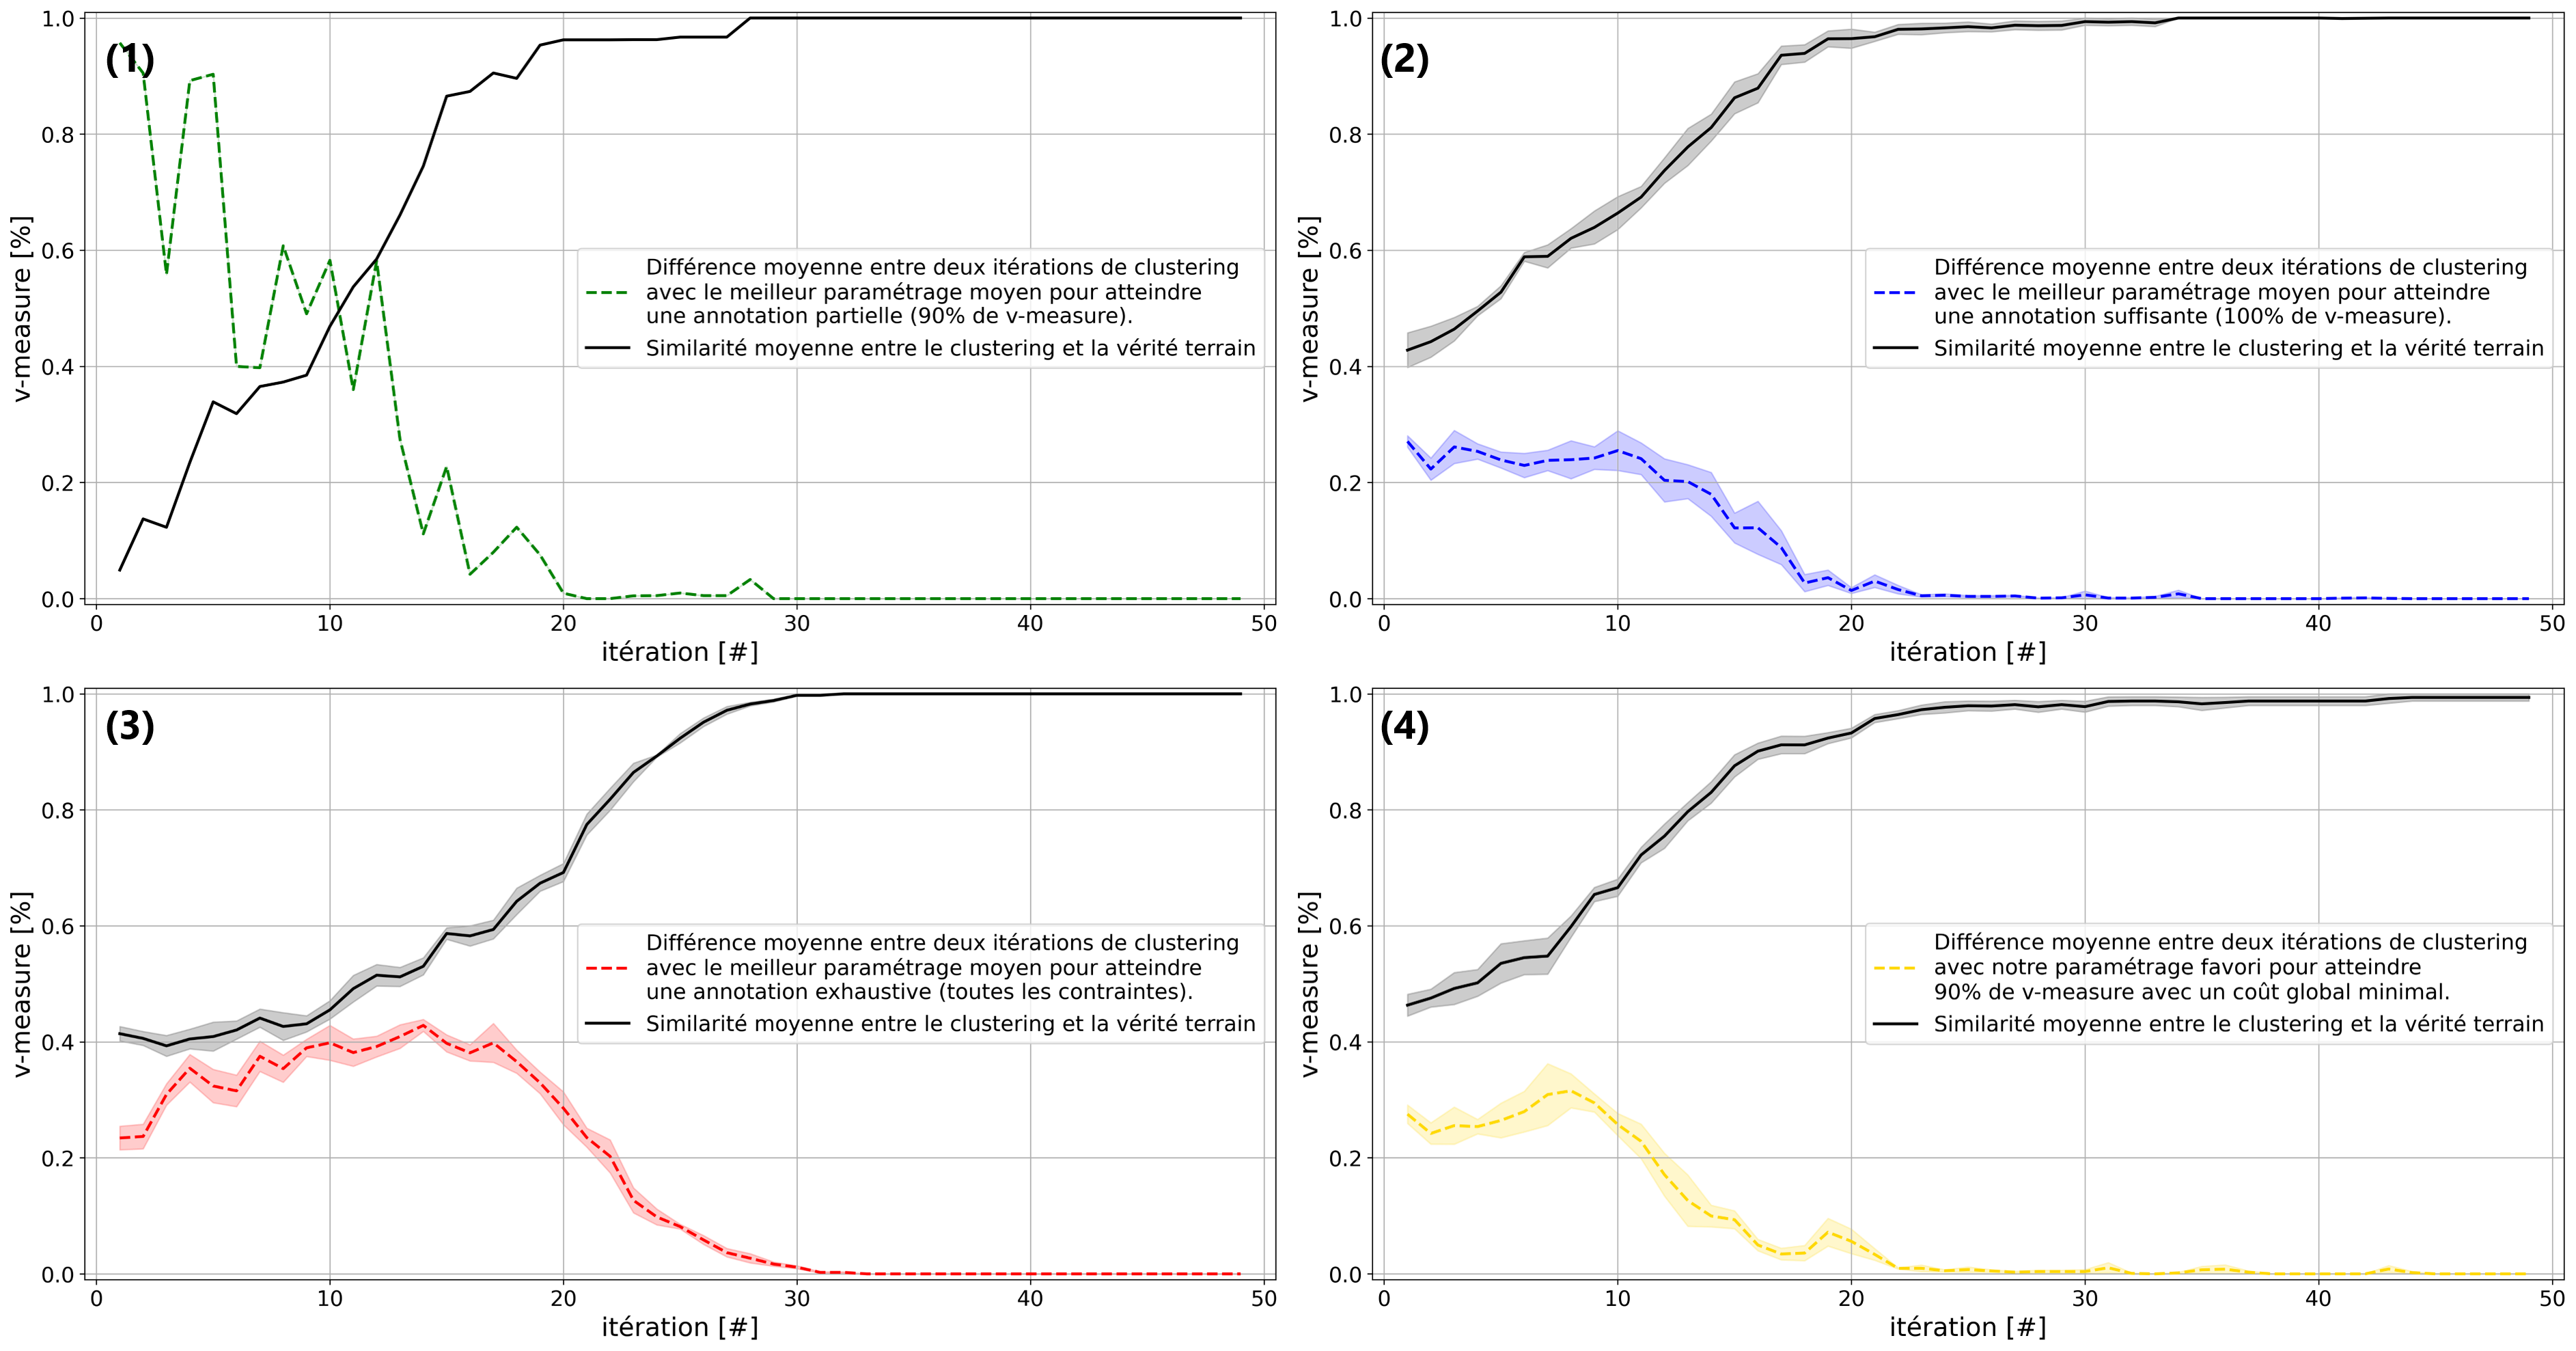
\includegraphics[width=0.95\textwidth]{figures/etude-rentabilite-similarite-clustering}
				\caption{
					Évolution de la différence de résultats entre deux itérations de \textit{clustering}.
					Les évolutions moyennes de différents paramétrages de la méthode sont exposées :
					\textbf{(1)} meilleur paramétrage moyen pour atteindre une annotation partielle ;
					\textbf{(2)} meilleur paramétrage moyen pour atteindre une annotation suffisante ;
					\textbf{(3)} meilleur paramétrage moyen pour atteindre une annotation exhaustive ;
					et \textbf{(4)} paramétrage favori.
					À titre d'information, les courbes en noir représentent l'évolution de la \texttt{v-measure} entre le \textit{clustering} et la vérité terrain.
				}
				\label{figure:4.5.2-ETUDE-RENTABILITE-SIMILARITE-CLUSTERING}
			\end{figure}
			
			% Tableau : corrélation forte.
			La \textsc{Table~\ref{table:4.5.2-ETUDE-RENTABILITE-CORRELATION-SIMILARITE-PERFORMANCE}} contient le score de corrélation entre cette différence et la performance théorique obtenue grâce à la vérité terrain.
			Cette corrélation est forte : $0.75$ sur l'ensemble des tentatives, $0.93$ sur les tentatives utilisant notre paramétrage favori.
			La \textsc{Figure~\ref{figure:4.5.2-ETUDE-RENTABILITE-SIMILARITE-CLUSTERING}} confirme cette corrélation :
			\begin{itemize}
				\item un score de \texttt{v-measure} avec la vérité terrain proche de $100$\% est accompagné d'un score de différence proche de $0$\% (après l'itération $20$ pour \textbf{(1)}, après l'itération $20$ pour \textbf{(2)}, après l'itération $30$ pour \textbf{(3)} et après l'itération $22$ pour \textbf{(4)}) ;
				\item une croissance de performance est généralement accompagnée d'un score non nul de différence (voir \textbf{(2)} et \textbf{(4)} entre les itérations $0$ et $20$), et plusieurs pics de performance sont accompagnés de scores forts de différence (particulièrement visible sur \textbf{(1)} vers l'itération $5$ et entre les itérations $10$ et $15$) ;
				\item il est toutefois à noter que l'inverse n'est pas vrai : un score non nul de différence n'accompagne pas forcément une croissance de performance, mais peut simplement caractériser un changement de partitionnement, comme c'est le cas dans \textbf{(3)} entre les itérations $0$ et $10$ où des modifications ont lieu (score de différence non nul) mais où la performance par rapport à la vérité terrain stagne.
			\end{itemize}
			%
			\begin{table}[!htb]
				\begin{center}
				\begin{tabular}{|c|r|}
				
					\hline
					% ENTETE DU TABLEAU
					\rowcolor{colorTableHeader!15}
					\multicolumn{1}{|c|}{\shortstack[c]{
						Paramétrage
					}}
						& \multicolumn{1}{c|}{\shortstack[c]{
							Corrélation
						}}
						\tabularnewline
						\hline \hline
					
					% Annotation partielle.
					Meilleur paramétrage moyen pour une annotation partielle \textbf{(1)}
						& $0.96$
						\tabularnewline
						\hline
					
					% Annotation suffisante.
					Meilleur paramétrage moyen pour une annotation suffisante \textbf{(2)}
						& $0.92$
						\tabularnewline
						\hline
					
					% Annotation exhaustive.
					Meilleur paramétrage moyen pour une annotation exhaustive \textbf{(3)}
						& $0.85$
						\tabularnewline
						\hline
					
					% Paramétrage favori
					Paramétrage favori \textbf{(4)}
						& $0.93$
						\tabularnewline
						\hline
					
					% Moyenne des $960$ tentatives.
					Moyenne des $960$ tentatives
						& $0.75$
						\tabularnewline
						\hline
					
				\end{tabular}
				\end{center}
				\caption{
					Score de corrélation \texttt{r} de \textit{Pearson} entre la performance du \textit{clustering} obtenu à l'aide d'une vérité terrain (\texttt{v-measure}) et le score de différence entre deux \textit{clustering} consécutifs.
				}
				\label{table:4.5.2-ETUDE-RENTABILITE-CORRELATION-SIMILARITE-PERFORMANCE}
			\end{table}
			
			% Description de la figure : autres paramétrages
			Les autres paramétrages représentés dans \textbf{(1)}, \textbf{(2)} et \textbf{(3)} comportent des tendances similaires (\textit{décroissance générale, forte corrélation avec la performance théorique}) à quelques détails près (\textit{\textbf{(1)} commence avec des scores de différence très forts avant de décroître avec de nombreux pics ; \textbf{(3)} croît légèrement avant d'entamer sa décroissance, ...}).
			
		%%% Discussion
		\subsubsection{Discussion}
		
			% Rappel de l'objectif : trouver un cas d'arrêt en regardant l'évolution de la différence entre deux \textit{clustering}.
			Dans cette étude, nous avons analysé l'évolution du score de différence entre deux itérations de \textit{clustering} dans l'espoir de définir un cas d'arrêt de notre méthodologie d'annotation qui soit indépendant d'une vérité terrain préétablie.
			
			% Avantage 1 : Caractérise la rentabilité.
			Tout d'abord, nous pouvons affirmer qu'il y a une forte corrélation entre l'évolution de ce score de différence et l'évolution du score de performance (voir \textsc{Table~\ref{table:4.5.2-ETUDE-RENTABILITE-CORRELATION-SIMILARITE-PERFORMANCE}} : \texttt{r} moyen de $0.75$ ; \texttt{r} supérieur à $0.85$ pour les paramétrages mis en avant).
			Cette corrélation est confirmée visuellement grâce à la \textsc{Figure~\ref{figure:4.5.2-ETUDE-RENTABILITE-SIMILARITE-CLUSTERING}} : plus les différences entre \textit{clustering} sont faibles, plus les performances des \textit{clustering} sont fortes.
			
			% Attention : Peut ne caractériser qu'un gros changement sans pour autant une amélioration.
			Un point d'attention est toutefois à retenir : une modification du partitionnement des données n'entraîne pas forcément un gain de performance (voir \textbf{(3)} entre les itérations $0$ et $10$ et \textbf{(4)} entre les itérations $0$ et $8$).
			Nous ne pouvons donc pas conclure que l'analyse de la différence entre deux itérations de \textit{clustering} permet de caractériser totalement la rentabilité d'une itération.
			
			% Avantage 2 : Permet de définir un cas d'arrêts.
			Cependant, nous pouvons tout de même nous servir de ce score pour définir un cas d'arrêt pour notre méthodologie d'annotation lorsque la différence entre deux \textit{clustering} est faible.
			Pour cela, il nous suffit de fixer un seuil bas du score de différence en dessous duquel il n'est plus rentable de faire de nouvelles itérations de la méthode car les performances ne s'améliorent plus significativement.
			Une analyse manuelle ou semi-manuelle (voir hypothèse de pertinence en \textsc{Section~\ref{section:4.4-HYPOTHESE-PERTINENCE}}) reste nécessaire pour confirmer la valeur métier du résultat obtenu.
			
			\begin{leftBarIdea}
				Si nous restons sur notre seuil théorique de $90$\% de \texttt{v-measure} (voir \textsc{Section~\ref{section:4.2-HYPOTHESE-EFFICIENCE}}) et que nous nous basons sur la \textsc{Figure~\ref{figure:4.5.2-ETUDE-RENTABILITE-SIMILARITE-CLUSTERING}} \textbf{(4)}, nous pouvons visuellement fixer ce seuil autour de $5$\% de différences.
				Le réglage fin de ce seuil pourra être le sujet de futures analyses complémentaires.
			\end{leftBarIdea}
			
			% Conclusions et suggestion.
			En conclusion, \textbf{le score de différences entre deux résultats de \textit{clustering} semble être un bon indicateur pour estimer un cas d'arrêt de notre méthodologie d'annotation}.
			Nous proposons d'utiliser un seuil par défaut de $5$\% pour implémenter ce cas d'arrêt.
			
	%%%
	%%% Subsection 4.5.3: Mise en commun des stratégies d'évaluation de la rentabilité d'une itération de la méthode et définition d'un cas d'arrêt indépendant d'une vérité terrain.
	%%%
	\subsection{Mise en commun des stratégies d'évaluation de la rentabilité d'une itération de la méthode et définition d'un cas d'arrêt indépendant d'une vérité terrain.}
	\label{section:4.5.3-ETUDE-RENTABILITE-MISE-EN-COMMUN}
			
		% Conclusion.
		\begin{leftBarSummary}
			Au cours de cette étude de rentabilité, nous avons pu voir que :
			\begin{itemize}
				\item[\itemko] l'analyse du score d'accord entre l'annotation courante et le \textit{clustering} précédent ne permet pas d'estimer la rentabilité d'une itération, ni de définir un cas d'arrêt de notre méthodologie d'annotation (cf. \textsc{Section~\ref{section:4.5.1-ETUDE-RENTABILITE-ACCORD-ANNOTATION-CLUSTERING}}) ;
				\item[\itemok] l'analyse des différences entre deux itérations de \textit{clustering} est une approche prometteuse pour estimer la rentabilité d'une itération (cf. \textsc{Section~\ref{section:4.5.2-ETUDE-RENTABILITE-SIMILARITE-CLUSTERING}}), bien qu'une modification significative entre deux résultats de \textit{clustering} n'implique pas forcément un gain de performance (\textit{les deux \textit{clustering} peuvent être différents mais avoir des \texttt{v-measure} avec la vérité terrain équivalentes}) ;
				\item[\itemok] l'usage de différences entre deux itérations de \textit{clustering} permet de définir un cas d'arrêt de notre méthodologie d'annotation : si les différences sont faibles (\textit{par exemple : inférieures à $5$\%}), alors les performances stagnent ou plafonnent ; il peut alors être intéressant d'interrompre le \texttt{Clustering Interactif} après avoir vérifié manuellement la pertinence des résultats obtenus (cf. \textsc{Section~\ref{section:4.4.4-ETUDE-PERTINENCE-MISE-EN-COMMUN}}).
			\end{itemize}
		\end{leftBarSummary}
		
		% Transition: Vers Simulation d'erreurs.
		Pour terminer nos différentes analyses, il convient maintenant d'anticiper la présence de différences d'annotation.
		En effet, nous avons fait jusqu'à présent l'hypothèse que l'annotateur ne se trompe jamais et que deux annotateurs n'ont jamais de désaccords, mais cette hypothèse forte n'est pas toujours vérifiée en pratique.
		Pour estimer l'impact de ces incohérences d'annotation, nous devons donc réaliser une analyse de robustesse de notre méthode d'annotation : celle-ci sera réalisée en \textsc{Section~\ref{section:4.6-HYPOTHESE-ROBUSTESSE}}.
	
	
	%%%%%--------------------------------------------------------------------
	%%%%% Section 4.6: Hypothèse de robustesse.
	%%%%%--------------------------------------------------------------------
	\newpage
	\section{Hypothèse de robustesse : « \textit{quelle influence d'une erreur ?} »}
\label{section:4.6-HYPOTHESE-ROBUSTESSE}

	%%% Formulation des hypothèses:
	Nous aimerions vérifier l'hypothèse suivante :
	\todo{à reformuler}

	\begin{tcolorbox}[
		title=\faVial~\textbf{Hypothèse de robustesse}~\faVial,
		colback=colorTcolorboxHypothesis!15,  % gray!20
		colframe=colorTcolorboxHypothesis!75,  % gray!50!black!75,
		width=\linewidth
	]
		« Il est possible d'\textbf{estimer l'influence d'une différence d'annotation} lors d'une méthodologie d'annotation basée sur le \textit{clustering} interactif (cf. figure~\ref{figure:4.6-HYPOTHESE-ROBUSTESSE}. »
		
		
		\begin{figure}[H]  % keep [H] to be in the tcolorbox.
			\centering
			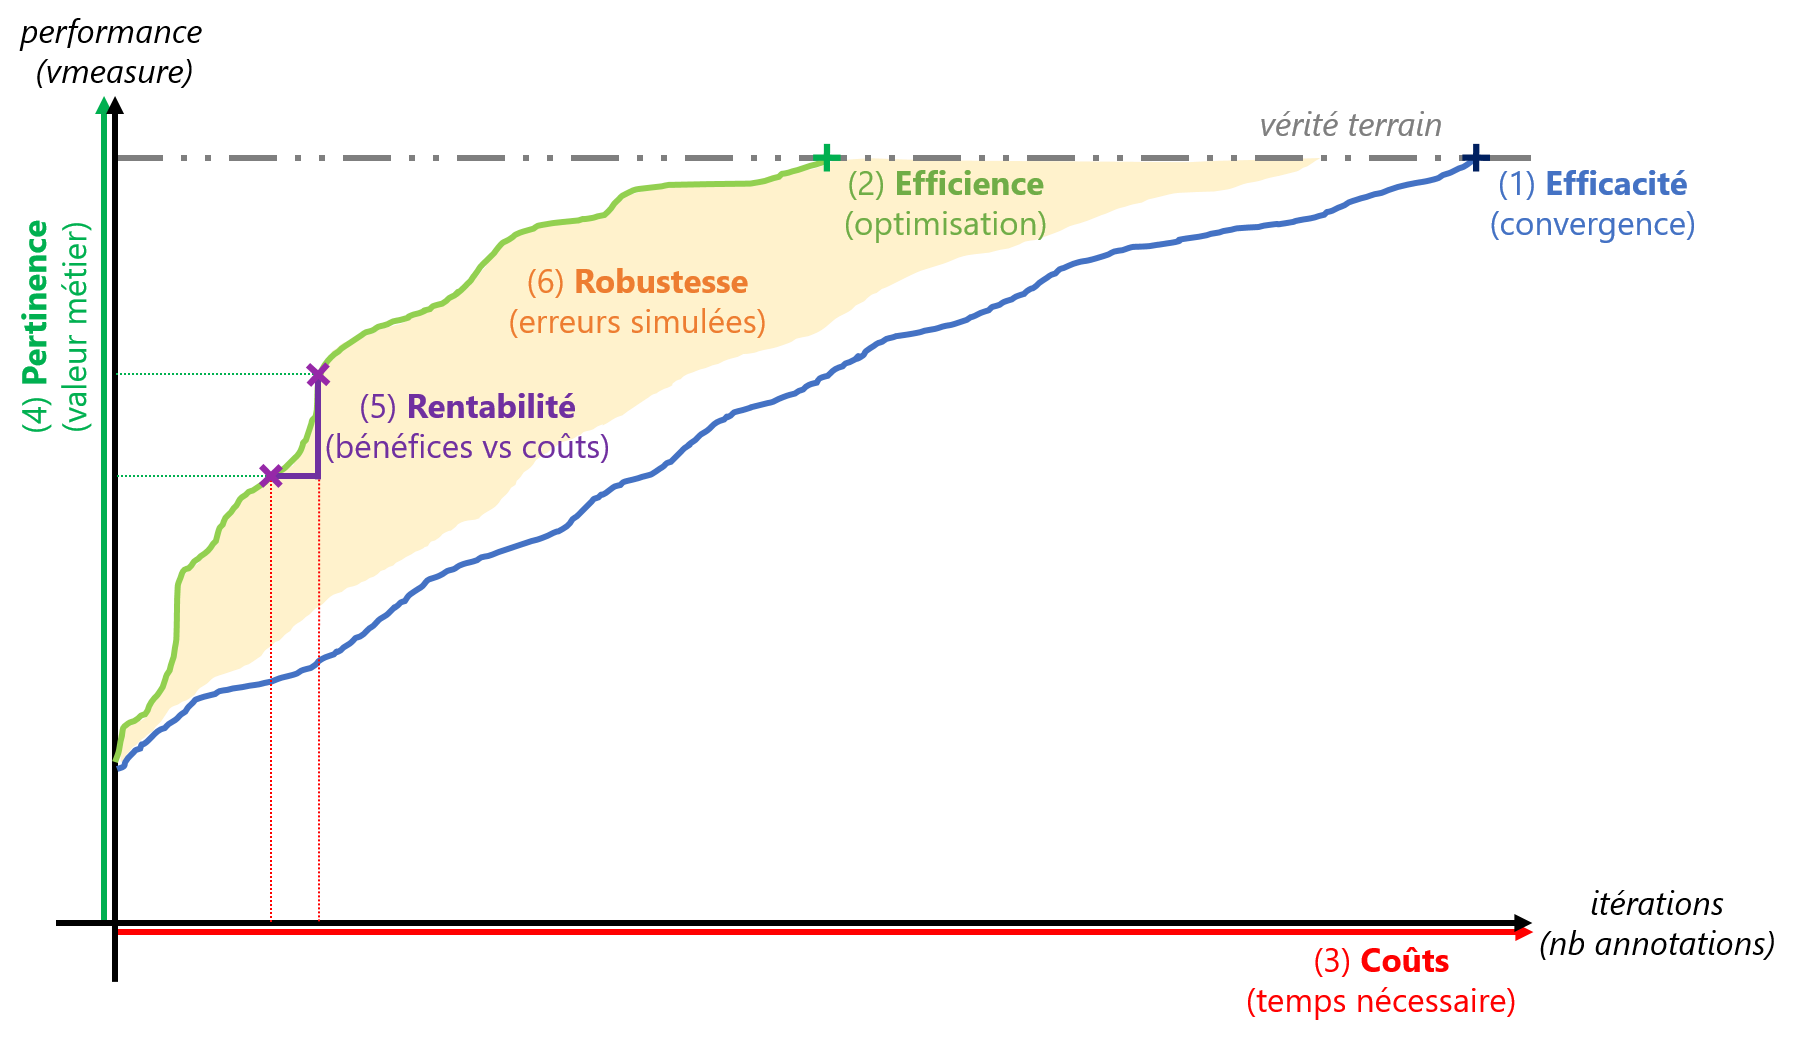
\includegraphics[width=0.95\textwidth]{figures/hypotheses-06-robustesse}
			\caption{Illustration des études réalisées sur le \textit{clustering} interactif (\textit{étape 6/6}) en schématisant l'évolution de la performance (\textit{accord avec la vérité terrain calculé en v-measure}) d'une base d'apprentissage en cours de construction en fonction du nombre d'itérations de la méthode (\textit{nombre d'annotations par un expert métier}).}
			\label{figure:4.6-HYPOTHESE-ROBUSTESSE}
		\end{figure}

	\end{tcolorbox}
	
	%%%
	%%% Subsection 4.6.1: Étude de simulation d'erreurs d'annotations
	%%%
	\subsection{Étude de simulation d'erreurs d'annotations}
	
		%%% Protocole expérimental.
		\subsubsection{Protocole expérimental}
			\todo[inline]{Description succincte du protocole expérimental dans l'encadré d'hypothèse ?}

		%%% Résultats
		\subsubsection{Résultats obtenus}

		%%% Discussion
		\subsubsection{Discussion}
	
	%%%
	%%% Subsection 4.6.2: Étude d'annotation avec des paradigmes différents
	%%%
	\subsection{Étude d'annotation avec des paradigmes différents}
	
		%%% Protocole expérimental.
		\subsubsection{Protocole expérimental}
			\todo[inline]{Description succincte du protocole expérimental dans l'encadré d'hypothèse ?}

		%%% Résultats
		\subsubsection{Résultats obtenus}

		%%% Discussion
		\subsubsection{Discussion}
	
	
	%%%%%--------------------------------------------------------------------
	%%%%% Section 4.7: Hypothèses non vérifiées.
	%%%%%--------------------------------------------------------------------
	\newpage
	\section{Autres hypothèses non vérifiées}
\label{section:4.7-HYPOTHESES-NON-VERIFIEES}

	%%%
	%%% Introduction / Transition.
	%%%
	Lors des études précédentes, nous avons vérifié un certain nombre d'hypothèses et avons exploré plusieurs détails pratiques pour mettre en oeuvre une méthodologie d'annotation basée sur le \textit{clustering} interactif.
	Toutefois, certains points n'ont pas pu être étudiés en profondeurs lors de ce doctorat, par manque de temps ou de moyens.
	Nous exposons ici un ensemble de pistes intéressantes pouvant nourrir de futurs travaux afin d'améliorer la notre méthode.
	
	
	%%%
	%%% Subsection 4.7.1: Étude du nombre de clusters optimal.
	%%%
	\subsection{Étude du nombre de clusters optimal}
	\label{section:4.7.1-HYPOTHESES-NON-VERIFIEES-NOMBRE-CLUSTERS}
	
		% Problème ouvert de la recherche: Estimer le nombre optimal de clusters.
		Un problème ouvert de la recherche lors de l'utilisation d'algorithmes de \textit{clustering} concerne le choix du nombre de \textit{clusters} à trouver.
		En effet, à part une connaissance à priori du nombre de thématiques présentes dans le jeu de données, il est difficile d'estimer le nombre optimal de \textit{clusters}, d'autant plus que celui-ci peut changer en fonction de la granularité de modélisation requise pour répondre au cas d'usage.
		
		% Pistes déjà explorées.
		Nous avons déjà exploré partiellement deux pistes :
		\begin{itemize}
			\item l'\textbf{exploration du graphe de contraintes} : en effet, il est possible d'estimer le nombre maximal de \textit{clusters} grâce aux composants connexes de contraintes \texttt{MUST-LINK}, et d'estimer le nombre minimal de \textit{clusters} grâce à la coloration du graphe de contraintes \texttt{CANNOT-LINK} ;
			\item les \textbf{études de pertinence} avec l'analyse des patterns linguistiques et le résumé thématique des \textit{clusters} (cf. \textsc{Section~\ref{section:4.4-HYPOTHESE-PERTINENCE}}) : ces deux approches permettent de rapidement constater si les thématiques obtenues sont trop générales (\textit{i.e. s'il n'y a pas assez de clusters}) ou si elles semblent trop spécifiques (\textit{i.e. s'il y en a trop}).
		\end{itemize}
		
		% Piste potentielles à explorer.
		Toutefois, pour aller plus loin, deux pistes potentielles pourraient être explorées :
		\begin{itemize}
			\item l'exploration brute du nombre de \textit{clusters} par la \textbf{méthode du coude} : bien que ces approches sont plus coûteuses en temps de calcul, elles permettent d'estimer le nombre de \textit{clusters} pour lequel la stabilité du \textit{clustering} est la plus élevée ;
			\item l'utilisation d'algorithme n'ayant pas de nombre de clusters en paramètres comme des versions contraintes de \texttt{DBScan} (par exemple dans sa version \texttt{C-DBScan}, \cite{ruiz-etal:2010:densitybased-semisupervised-clustering}) ou de la \textbf{propagation par affinité} (\cite{givoni-frey:2009:semisupervised-affinity-propagation}) : ces alternatives semblent prometteuses car elles retirent la complexité due à ce paramétrage abstrait.
		\end{itemize}
		
		\setcounter{localCounterOfFootnoteValue}{\value{footnote}}
		\begin{leftBarInformation}
			L'étude de \texttt{C-DBScan} a été en partie réalisée dans le cadre d'un projet étudiant avec l'école d'ingénieur Télécom Physique Strasbourg.
			Les résultats montraient que le temps de calcul était similaire à celui du \texttt{KMeans} (dans sa version \texttt{COP}).
			La difficulté d'utilisation résidait plutôt sur la définition du rayon de voisinage \texttt{eps} à parcourir pour établir des liens entre données.
			Celui-ci peut être estimé en analysant la densité vectorielle du jeu de données.
			Le code informatique est disponible dans \cite{schild:2022:cognitivefactory-interactiveclustering} \footnotemark.
		\end{leftBarInformation}
		% Rattraper les footnote.
			\stepcounter{localCounterOfFootnoteValue}
			\footnotetext[\value{localCounterOfFootnoteValue}]{
				Implémentation de \texttt{C-DBScan} : \textit{Pull Request} en attente pour une version \texttt{0.6.0} après ajout de documentation et de tests unitaires.
			}
	
	
	%%%
	%%% Subsection 4.7.2: Étude d'autres méthodes de vectorisation.
	%%%
	\subsection{Étude d'autres méthodes de vectorisation}
	\label{section:4.7.2-HYPOTHESES-NON-VERIFIEES-VECTORISATION}
	
		% Introduction.
		Au début de ce doctorat, nous avons conclu que les algorithmes de vectorisation n'avaient pas d'impact réel sur l'efficience de notre méthodologie d'annotation.
		Toutefois, les modèles de langues se sont largement développés, et il est fort probable que l'utilisation d'un \textbf{modèle pré-entraîné} permettent désormais d'avoir un gain de performance.
		
		% Piste potentielles à explorer.
		Nous pourrions par exemple tester les \textbf{architectures à base de \textit{Transformers}} (\cite{uszkoreit:2017:transformer-novel-neural}) comme \texttt{BERT} (\cite{devlin-etal:2019:bert-pretraining-deep}) et essayer différents modèles pré-entraînés sur des données françaises pour compléter nos études réalisées dans \cite{schild:2021:cognitivefactory-interactiveclusteringcomparativestudy}
	
	
	%%%
	%%% Subsection 4.7.3: Étude d'autres méthodes d'échantillonnage.
	%%%
	\subsection{Étude d'autres méthodes d'échantillonnage}
	\label{section:4.7.3-HYPOTHESES-NON-VERIFIEES-ECHANTILLONNAGE}
	
		% Introduction.
		Comme nous avons pu le voir dans \textsc{Section~\ref{section:4.6-HYPOTHESE-ROBUSTESSE}}, il peut-être intéressant d'introduire un mécanisme de création de redondance dans le graphe de contraintes annotées pour identifier les erreurs d'annotation.
		Un tel mécanisme n'a pas encore été implémenté mais pourrait facilement être intégré aux implémentations \texttt{Python} déjà existantes (\cite{schild:2022:cognitivefactory-interactiveclustering}).
		
		% Piste potentielles à explorer.
		Pour ce faire, le parcours de graphe et la création de cycle permettraient de vérifier la présence de conflits et ainsi de \textbf{provoquer des phases de revues de contraintes} si cela est nécessaire.
		Une telle page de revue pourrait aussi être complétée par des analyses complémentaires, comme l'estimation du taux de contraintes n'ayant pas de redondance et représentant ainsi des erreurs cachées potentielles.
	
	
	%%%
	%%% Subsection 4.7.4: Étude de techniques de transfert d'apprentissage.
	%%%
	\subsection{Étude de techniques de transfert d'apprentissage}
	\label{section:4.7.4-HYPOTHESES-NON-VERIFIEES-TRANSFERT-APPRENTISSAGE}
	
		% Introduction.
		Dans la \textsc{Section~\ref{section:2.3-DEFIS-ANNOTATION}}, nous avions déjà évoqué le fait que la modélisation d'un phénomène peut être assister par des techniques telles que la pré-annotation (\cite{dandapat-etal:2009:complex-linguistic-annotation}) ou le transfert d'apprentissage (\cite{zhuang-etal:2021:comprehensive-survey-transfer}).
		Nous pourrions nous inspirer davantage de ces approches pour démarrer plus efficacement les premières itérations d'un \textit{clustering} interactif.
	
		% Piste potentielles à explorer.
		Voici quelques idées inspirées de ces méthodes :
		\begin{itemize}
			\item \textbf{pré-annoter} certaines contraintes simples à l'aide de règles (\textit{basées par exemple sur la présence de mots de vocabulaire en commun}) ou grâce à l'utilisation d'un modèle déjà disponible ; 
			\item \textbf{introduire des données synthétiques ou empruntées} à d'autres bases d'apprentissage pour initialiser le \textit{clustering}, et permettre ainsi ajouter d'emblée des connaissances générales dans la modélisation.
		\end{itemize}
	
	
	%%%
	%%% Subsection 4.7.5: Étude ergonomique de l'interface d'annotation.
	%%%
	\subsection{Étude ergonomique de l'interface d'annotation}
	\label{section:4.7.5-HYPOTHESES-NON-VERIFIEES-ERGONOMIQUE}
	
		% Introduction.
		L'application web développée au cours de ce doctorat (\cite{schild-etal:2022:cognitivefactory-interactiveclusteringgui}) permet d'essayer rapidement notre méthodologie d'annotation.
		Cependant, cette dernière n'a pu faire l'objet d'études poussées pour estimer la meilleure disposition des composants ou l'intérêt de certaines fonctionnalités d'annotation.
		
		% Piste potentielles à explorer.
		Parmi les pistes potentielles à explorer, nous avons évoqué la possibilité d'\textbf{annoter plusieurs contraintes} dans une même interface (\textit{par exemple : annoter visuellement un mini-graphes de $4$ données plutôt que d'annoter simplement un couple de données}) et le besoin de \textbf{réaliser des analyses rapides} sur les \textit{clusters} ou sur le graphe de contraintes (voir \textsc{Section~\ref{section:4.4-HYPOTHESE-PERTINENCE}} et \textsc{Section~\ref{section:4.5-HYPOTHESE-RENTABILITE}}).
		Pour aller plus loin, \cite{bae-etal:2021:interactive-clustering-comprehensive} propose d'autres listes d'interactions qui sont possibles d'avoir avec un algorithmes de \textit{clustering}, notamment sur la manipulation de son résultats (\textit{fusion, suppression, verrouillage, ...}) et de ses hyperparamètres (\textit{nombre de \textit{clusters}, adaptation du vocabulaire autorisé, ...})
		
		% A essayer !
		Toutes ces idées pourraient être l'objet de développements et d'études dédiées avec des groupes d'annotateurs différentes pour voir l'impact sur les performances et les biais de conception de modèles.
	
	
	%%%%%--------------------------------------------------------------------
	%%%%% Section 4.8: Bilan des études réalisées
	%%%%%--------------------------------------------------------------------
	%\newpage
	%\section{Bilan des études réalisées}
\label{section:4.8-BILAN-HYPOTHESES}
	\todo[inline]{SECTION À RÉDIGER}
	
	% FONCTIONNALITES
		% trouver une base d'apprentissage acceptable, puis corriger manuellement
		% intervention d'experts métiers sur la base de leur connaissance métiers
		% revues d'annotations basée sur leur connaissance métiers
		% adaptation de la modélisation faite par le clustering
	
	% PARAMETRAGES
		% Architecture parallele :
		% paramétrage :
		% batch_size :
	
	% ANALYSE
		% Cas d'arrêt quand le clustering stage à +/- 5%
		% Analyse avec FMC + résumé LLM
	
	% COUTS
		% equations de temps
		% besoin de 3 annotateurs
		% ajouter de la redondance si le cas d'usage est complexe

%%%%%--------------------------------------------------------------------
%%%%% Chapitre: Guide d'utilisation
%%%%%--------------------------------------------------------------------
\chapter{Guide d'utilisation du \textit{Clustering Interactif}}
\label{chapter:5-GUIDE}

	%%%%%--------------------------------------------------------------------
	%%%%% Section 5.1:
	%%%%%--------------------------------------------------------------------
	\section{Organisation \texttt{ITTER}}
		\label{section:5.1-GUIDE-ITTER}
		\todo[inline]{SECTION À RÉDIGER}
	
	
	%%%%%--------------------------------------------------------------------
	%%%%% Section 5.2:
	%%%%%--------------------------------------------------------------------
	\section{Conseils pratiques}
		\label{section:5.2-GUIDE-CONSEILS}
		\todo[inline]{SECTION À RÉDIGER}

%%%%%--------------------------------------------------------------------
%%%%% Conclusion
%%%%%--------------------------------------------------------------------
\chapter{Conclusion}
\label{chapter:6-CONCLUSION}
	
	%%%%%--------------------------------------------------------------------
	%%%%% OCCUPYING THE NICHE: Proposition d'une méthode d'annotation valorisant l'expertise métier.
	%%%%%--------------------------------------------------------------------
	\section*{Proposition d'une nouvelle méthode d'annotation valorisant l'expertise métier}
	\addcontentsline{toc}{section}{
		\protect\numberline{}
		Proposition d'une nouvelle méthode d'annotation valorisant l'expertise métier
	}
	
		%%% Introduction, Revue de littérature et Rappel de la problématique (voir \textsc{Chapitre~\ref{chapter:2-REVUE-DE-LITTERATURE}}).
		Dans cette thèse, nous nous sommes intéressé à la tâche d'annotation, nécessaire à l'entraînement d'assistants conversationnels, et impliquant habituellement des experts du domaine à modéliser.
		Lors de notre revue de littérature, nous avons pu constater que l'annotation avait la réputation d'être une tâche complexe et subjective.
		Cette complexité provient notamment du besoin d'avoir des données représentatives du phénomène à reproduire, exerçant par conséquent une forte pression quant à la qualité de la base d'apprentissage à construire.
		Un projet d'annotation s'organise alors traditionnellement autour du cycle \texttt{MATTER}, une méthodologie durant laquelle la modélisation des textes en intentions est révisée plusieurs fois pour mieux s'adapter aux données du projet.
		Cependant, une telle organisation se révèle généralement coûteuse, entre autres à cause des nombreux ateliers de modélisation en mode essai-erreur, de la difficulté à manipuler des concepts abstraits (\textit{intentions}, \textit{entités}, ...), et du besoin de former les experts aux tâches d'analyse.
		Sur la base de ces constats, nous avons cherché une méthodologie d'annotation alternative en nous posant la question suivante : \textguillemets{\textbf{Comment assister la phase de modélisation de textes en intentions pour concevoir la base d'apprentissage d'un assistant conversationnel en impliquant des experts métiers pour leurs vraies compétences et en leur demandant un minimum de bagages analytiques ou techniques ?}}
		
		%%% Rappel proposition \texttt{Clustering Interactif} (voir \textsc{Chapitre~\ref{chapter:3-CLUSTERING-INTERACTIF}}).
		En choisissant de mettre l'accent sur les connaissances réelles des experts, nous avons proposé une approche de modélisation des textes en intentions utilisant un \texttt{Clustering Interactif}.
		Cette méthodologie repose sur la coopération entre l'Homme et la Machine :
		\begin{itemize}
			\item d'une part, la machine réalise un \textit{clustering} pour proposer une base initiale d'apprentissage ;
			\item d'autre part, l'expert métier annote des contraintes binaires entre les données dans le but d'affiner itérativement la base d'apprentissage proposée.
		\end{itemize}
		Une telle approche a l'avantage d'être plus instinctive, car les experts peuvent associer ou différencier les données en fonction de la similarité de leur cas d'usage, permettant ainsi de traiter les données comme ils le feraient professionnellement au quotidien.
		De plus, cette méthodologie définie clairement les rôles entre les parties : l'expert métier intervient uniquement pour transmettre ses connaissances métiers, et la machine se charge d'appliquer cette connaissance pour concevoir une modélisation stable et pertinente des textes en intentions.
		
		
		%%% Rappel études sur le \texttt{Clustering Interactif} (voir \textsc{Chapitre~\ref{chapter:4-ETUDES}}).
		Pour éprouver notre méthodologie d'annotation, nous avons réalisé un ensemble d'études réparties en six hypothèses : efficacité, efficience, coûts, pertinence, rentabilité et robustesse.
		Grâce à ces études, nous avons pu démontrer que notre méthode diminuait sensiblement la complexité de conception d'une base d'apprentissage, réduisant notamment la nécessité de formation des experts intervenant dans un projet d'annotation.
		Nous mettons à disposition une implémentation technique de cette méthode (algorithmes et interface graphique associée), ainsi qu'une étude des paramètres optimaux pour obtenir une base d'apprentissage cohérente en un minimum d'annotations (hypothèse d'efficacité et d'efficience).
		Nous réalisons également une étude de coûts (techniques et humains) permettant de confirmer que l'utilisation d'une telle méthode est réaliste dans un cadre industriel.
		Les trois dernières hypothèses (pertinence, rentabilité et robustesse) permettent de vérifier le comportement et les limites de notre technique, ouvrant ainsi la discussion sur les fonctionnalités et mécanismes de suivi nécessaires à sa mise en oeuvre.
		
		%%% Rappel guide sur le \texttt{Clustering Interactif} (voir \textsc{Chapitre~\ref{chapter:5-GUIDE}}).
		Nous dressons ensuite le bilan de notre méthodologie d'annotation sous la forme d'un guide d'utilisation synthétique.
		Afin que la méthode atteigne son plein potentiel, nous y fournissons un ensemble de conseils, notamment : (1) des recommandations visant à cadrer la stratégie d'annotation, (2) une aide à l'identification et à la résolution des divergences d'opinion entre annotateurs, (3) des indicateurs de rentabilité pour chaque intervention de l'expert, et (4) des méthodes d'analyse de la pertinence de la base d'apprentissage en cours de construction.
		
		%%% Conclusion finale.
		En conclusion, notre méthodologie d'annotation représente une réelle alternative aux stratégies d'annotation traditionnelles, permettant de valoriser les annotateurs pour les compétences qu'ils possèdent, et non pour les compétences dont le projet d'annotation a besoin.
		
		
	%%%%%--------------------------------------------------------------------
	%%%%% NICHE and ASSET CENTRALITY: Perspectives d'utilisation du \textit{Clustering Interactif}.
	%%%%%--------------------------------------------------------------------
	\section*{Perspectives d'utilisation du \textit{Clustering Interactif}}
	\addcontentsline{toc}{section}{
		\protect\numberline{}
		Perspectives d'utilisation du \textit{Clustering Interactif}
	}
		
		%%% Amélioration signification de l'implication des experts métiers.
		Nous avons pu montrer que cette thèse offrait une approche innovante pour concevoir une base d'apprentissage d'un assistant conversationnel, permettant d'impliquer les experts du domaine métier pour leurs vraies connaissances, tout en leur demandant un minimum de compétences analytiques et techniques.
		En effet, ces travaux prouvent qu'il est possible de contourner habillement la complexité d'une tâche d'annotation en reformulant judicieusement le problème exposé à l'annotateur, ouvrant ainsi la voie à des méthodes plus accessibles pour construire ces assistants.

		%%% Certes moins pour la gestion de dialogues (cf \textit{chatbot} génératif), mais probablement pour leur contrôle ; Application possible à des domaines autre que le texte (image, voix, données tabulaires, ...) si la modélisation est complexe
		Néanmoins, depuis $2023$, la conception de \textit{chatbot} s'est davantage tournée vers les approches génératives, celles-ci n'ayant plus besoin d'intentions pour gérer le dialogue.
		Mais malgré leurs performances encourageantes, ces approches manquent encore clairement de fiabilité, notamment en ce qui concerne les dérives de comportements et les risques d'hallucination ; de plus, une étape de modélisation reste nécessaire pour paramétrer certaines de leurs actions spécifiques (\textit{allumer la lumière, lancer un appel téléphonique, faire un virement bancaire, ...}).
		De ce fait, nous pensons que notre approche reste pertinente pour entraîner des assistants orientés par tâches, pour modéliser des mécanismes de contrôle, ou encore pour assister la conception de certains assistants hybrides.
		D'autre part, notre approche peut facilement se généraliser à d'autres cas d'usages faisant intervenir une classification supervisée (\textit{classification d'images, de documents, ...}).
		
		%%% Mot d'ordre de la fin.
		Pour conclure ce manuscrit, nous encourageons les gérants de projets d'annotation, quelle que soit la tâche d'annotation à réaliser, à repenser leur protocole de labellisation de données en considérant d'abord les vraies connaissances de leurs experts.
		En effet, il est tentant de concevoir une stratégie d'annotation classique, et de supposer qu'un annotateur "parfait" ou suffisamment formé arrivera à en supporter la complexité.
		Cependant, nous avons montré au cours de ce doctorat qu'en reformulant judicieusement l'objectif, il était possible de concevoir une stratégie d'annotation accessible facilement aux experts du domaine métier, faisant appel à des connaissances qu'ils appliquent professionnellement au quotidien.
		Par conséquent, nous pensons qu'il est de notre ressort de réexaminer l'organisation de nos projets d'annotation, afin de ne pas avoir à former des experts pour des tâches qu'ils ne maîtrisent pas, mais de les impliquer pour des tâches où ils sont déjà des experts : un tel changement de position serait alors une réelle avancée pour les annotateurs intervenant dans des projets d'apprentissage automatique.


%%%%%%%%%%%%%%%%%%%%%%%%%%%%%%%%%%%%%%%%%%%%%%%%%%%%%%%%%%%%%%%%%%%%%%%
%%%%% ANNEXES
%%%%%%%%%%%%%%%%%%%%%%%%%%%%%%%%%%%%%%%%%%%%%%%%%%%%%%%%%%%%%%%%%%%%%%%

\PutLineInToc
\Annexes

%%%%%--------------------------------------------------------------------
%%%%% Annexe A: JEUX DE DONNÉES
%%%%%--------------------------------------------------------------------
%\newpage
\DontFrameThisInToc
\Annex{Annexe des jeux de données utilisés dans nos études}
\label{annex:A-ANNEXE-DATASET}

	% INTRODUCTION DE L'ANNEXE.
	Pour les différentes études réalisées au cours de ce doctorant (cf. \textsc{Chapitre~\ref{chapter:4-ETUDES}}), nous avons utilisé les deux jeux de données suivants.

	% TABLE DES MATIÈRES DE L'ANNEXE.
	\minitoc


	%%%%%--------------------------------------------------------------------
	%%%%% Annexe A.1: \texttt{Bank Cards}: Jeu d'entraînement en français d'assistants conversationnels traitant des demandes courantes sur les cartes bancaires
	%%%%%--------------------------------------------------------------------
	\newpage
	\section[
		Jeu de données \texttt{Bank Cards}
	]{
		\texttt{Bank Cards}: Jeu d'entraînement en français d'assistants conversationnels traitant des demandes courantes sur les cartes bancaires
	}
	\label{annex:A.1-DATASET-BANK-CARDS}
		
		
		% Description.
		\paragraph{Description :}
		Cet ensemble de données représente des exemples de demandes usuelles des clients concernant la gestion des cartes bancaires.
		Il peut être utilisé comme jeu d'entraînement pour un petit assistant conversationnel destiné à traiter ces demandes courantes.
		
		% Contenu.
		\paragraph{Contenu :}
		Les questions sont formulées en français.
		L'ensemble de données est divisé en $10$ intentions (classes) dont un aperçu est disponible dans la \textsc{Table~\ref{table:A.1-DATASET-BANK-CARDS}}.
		Ces intentions sont construites de telle manière que toutes les questions issues d'une même intention ont la même réponse ou action.
		La version \texttt{1.0.0} du jeu de données contient de $50$ questions par intention, soit un total de $500$ questions ;
		La version \texttt{2.0.0} du jeu de données contient de $100$ questions par intention, soit un total de $1~000$ questions.
		
		\begin{table}[!htb]
			\begin{center}
			\begin{scriptsize}
			\begin{tabular}{|c|c|c|c|}
			
				\hline
				% ENTETE DU TABLEAU
				\rowcolor{colorTableHeader!15}
				\textbf{Intention}
					& \textbf{Définition}
					& \textbf{Exemple}
					\tabularnewline
					\hline \hline
				% alerte\_perte\_vol\_carte
				\multirow{2}{*}{\texttt{alerte\_perte\_vol\_carte}}
					& Affichage de la procédure de blocage
					& \textit{Comment signaler une perte}
					\tabularnewline
					& d'une carte perdue ou volée
					& \textit{de carte de paiement ?}
					\tabularnewline
					\hline
				% carte\_avalee
				\multirow{2}{*}{\texttt{carte\_avalee}}
					& Affichage de la procédure de
					& \textit{Comment récupérer}
					\tabularnewline
					& récupération d'une carte avalée
					& \textit{une carte avalée ?}
					\tabularnewline
					\hline
				% commande\_carte
				\multirow{2}{*}{\texttt{commande\_carte}}
					& Affichage des cartes disponibles,
					& \textit{Je souhaite changer}
					\tabularnewline
					& de la procédure de commande,
					& \textit{de carte bancaire.}
					\tabularnewline
					\hline
				% consultation\_solde
				\multirow{2}{*}{\texttt{consultation\_solde}}
					& Affichage d'une synthèse des
					& \textit{Où retrouver le solde}
					\tabularnewline
					& soldes bancaires du client.
					& \textit{ de mon compte ?}
					\tabularnewline
					\hline
				% couverture\_assurrance
				\multirow{2}{*}{\texttt{couverture\_assurrance}}
					& Affichage d'une synthèse des garanties
					& \textit{Que couvre ma carte bancaire}
					\tabularnewline
					& d'assurances de la carte bancaire du client
					& \textit{en cas d'hospitalisation ?}
					\tabularnewline
					\hline
				% deblocage\_carte
				\multirow{2}{*}{\texttt{deblocage\_carte}}
					& Affichage de gestion du statut
					& \textit{ma carte de paiement est}
					\tabularnewline
					& des cartes du client.
					& \textit{bloquée, que faire ?}
					\tabularnewline
					\hline
				% gestion\_carte\_virtuelle
				\multirow{2}{*}{\texttt{gestion\_carte\_virtuelle}}
					& Affichage de gestion des cartes
					& \textit{Comment faire pour créer une}
					\tabularnewline
					& virtuelles du client.
					& \textit{carte de paiements virtuelle ?}
					\tabularnewline
					\hline
				% gestion\_decouvert
				\multirow{2}{*}{\texttt{gestion\_decouvert}}
					& Affichage d'une synthèse des autorisations
					& \textit{Est-ce que j'ai un}
					\tabularnewline
					& de découverts de leur procédure de gestion
					& \textit{découvert autorisé ?}
					\tabularnewline
					\hline
				% gestion\_plafond
				\multirow{2}{*}{\texttt{gestion\_plafond}}
					& Affichage de gestion des plafonds
					& \textit{Le plafond de ma carte est}
					\tabularnewline
					& des cartes du client.
					& \textit{trop bas, que faire ?}
					\tabularnewline
					\hline
				% gestion\_sans\_contact
				\multirow{2}{*}{\texttt{gestion\_sans\_contact}}
					& Affichage de gestion des
					& \textit{Je veux désactiver le}
					\tabularnewline
					& fonctionnalités des cartes du client.
					& \textit{sans contact sur ma carte.}
					\tabularnewline
					\hline
			\end{tabular}
			\end{scriptsize}
			\end{center}
			\caption{
				Présentation du jeu de données \texttt{Bank Cards} avec quelques exemples.
				La version \texttt{2.0.0} contient $100$ questions par intention.
			}
			\label{table:A.1-DATASET-BANK-CARDS}
		\end{table}
		
		% Origine.
		\paragraph{Origine :}
		Le périmètre des intentions est inspiré d'un chatbot actuellement en production.
		Les données ont été sélectionnées aléatoirement et reformulées manuellement pour garantir la confidentialité des utilisateurs : aucune données personnelles ne subsistent dans ce jeu de données.
		Enfin, deux réviseurs extérieurs à l'équipe de recherche (\textit{des Data Analyst}), ayant un profil d'analystes métiers du domaine bancaire, ont validé le périmètre et le contenu de ces intentions.
		
		% Disponibilité.
		\paragraph{Disponibilité :}
		Le jeu de données est archivé sur la plateforme \texttt{Zenodo} et est accessible ici: \cite{schild:2022:french-trainset-chatbots}


	%%%%%--------------------------------------------------------------------
	%%%%% Annexe A.2: \texttt{MLSUM} (The Multilingual Summarization Corpus): Échantillon de titres d'articles de journaux en français associés à leur classification thématique
	%%%%%--------------------------------------------------------------------
	\newpage
	\section[
		Jeu de données \texttt{MLSUM}
	]{
		\texttt{MLSUM} (The Multilingual Summarization Corpus): Échantillon de titres d'articles de journaux en français associés à leur classification thématique
	}
	\label{annex:A.2-DATASET-MLSUM-SUBSET-SCHILD}
		
		
		% Description.
		\paragraph{Description :}
		C'est un ensemble d'articles de journaux avec leur titre, leur résumé et leur classification thématique.
		Nous l'utilisons (1) pour estimer le temps nécessaire pour annoter la similarité des titres avec des contraintes (\texttt{MUST-LINK}, \texttt{CANNOT-LINK}) et (2) pour tester la méthodologie de \texttt{Clustering Interactif} (annotation de contraintes et \textit{clustering} sous contraintes).
		
		% Contenu.
		\paragraph{Contenu :}
		Les titres de journaux sont formulés en français.
		L'ensemble de données est divisé en $14$ thèmes (classes) dont un aperçu est disponible dans la \textsc{Table~\ref{table:A.2-DATASET-MLSUM-SUBSET-SCHILD}}.
		La version \texttt{1.0.0 [subset: fr+train+filtered]} contient $744$ articles.
		
		\begin{table}[!htb]
			\begin{center}
			\begin{scriptsize}
			\begin{tabular}{|c|c|c|c|}
			
				\hline
				% ENTETE DU TABLEAU
				\rowcolor{colorTableHeader!15}
				\textbf{Thème}
					& \textbf{Définition}
					& \textbf{Exemple}
					& \textbf{Taille}
					\tabularnewline
					\hline \hline
				% arts
				\multirow{2}{*}{\texttt{arts}}
					& Actualités artistiques (spectacles,
					& \textit{La rencontre de l'art et de la }
					& \multirow{2}{*}{$50$}
					\tabularnewline
					& oeuvres, événements, expositions)
					& \textit{gastronomie au château du Feÿ}
					&
					\tabularnewline
					\hline
				% disparitions
				\multirow{2}{*}{\texttt{disparitions}}
					& Actualités nécrologiques 
					& \textit{Le traducteur Jean-Pierre}
					& \multirow{2}{*}{$48$}
					\tabularnewline
					& (décès ou disparition)
					& \textit{Carasso est mort à 73 ans}
					&
					\tabularnewline
					\hline
				% ecologie
				\multirow{2}{*}{\texttt{ecologie}}
					& Actualités sur la pollution
					& \textit{Comment Lyon a banni les}
					& \multirow{2}{*}{$34$}
					\tabularnewline
					& et la transition écologique
					& \textit{pesticides de ses parcs et jardins}
					&
					\tabularnewline
					\hline
				% economie
				\multirow{2}{*}{\texttt{economie}}
					& Actualités économiques,
					& \textit{La guerre des prix s'intensifie}
					& \multirow{2}{*}{$41$}
					\tabularnewline
					& financières et boursières
					& \textit{sur le marché du mobile en Israël}
					&
					\tabularnewline
					\hline
				% education
				\multirow{2}{*}{\texttt{education}}
					& Actualités liées à l'éducation
					& \textit{Plainte de parents d'élève sur des notes}
					& \multirow{2}{*}{$62$}
					\tabularnewline
					& et à la filière enseignante
					& \textit{jugées trop basses au bac}
					&
					\tabularnewline
					\hline
				% emploi
				\multirow{2}{*}{\texttt{emploi}}
					& Actualités liées au marché du
					& \textit{Plus d'un tiers des CDI prennent}
					& \multirow{2}{*}{$54$}
					\tabularnewline
					& travail et aux actions syndicales
					& \textit{ fin avant la première année}
					&
					\tabularnewline
					\hline
				% immobilier
				\multirow{2}{*}{\texttt{immobilier}}
					& Actualités liées au marché de
					& \textit{Depuis la fin des années 2000, l'accession}
					& \multirow{2}{*}{$65$}
					\tabularnewline
					& l'immobilier et logements locatifs
					& \textit{à la propriété se complique en France}
					&
					\tabularnewline
					\hline
				% meteo
				\multirow{2}{*}{\texttt{meteo}}
					& Actualités météorologiques
					& \textit{L'Eure et l'est de la France}
					& \multirow{2}{*}{$35$}
					\tabularnewline
					& (bulletins, catastrophes, canicule)
					& \textit{balayés par les intempéries}
					&
					\tabularnewline
					\hline
				% musiques
				\multirow{2}{*}{\texttt{musiques}}
					& Actualités liées aux chanteurs,
					& \textit{Opéra : Elsa Dreisig,}
					& \multirow{2}{*}{$55$}
					\tabularnewline
					& concerts et sorties d'albums
					& \textit{une soprano à voix nue}
					&
					\tabularnewline
					\hline
				% police-justice
				\multirow{2}{*}{\texttt{police-justice}}
					&Actualités liées aux affaires
					& \textit{Bygmalion : Nicolas Sarkozy}
					& \multirow{2}{*}{$67$}
					\tabularnewline
					& policières et aux tribunaux
					& \textit{directement visé}
					&
					\tabularnewline
					\hline
				% politique
				\multirow{2}{*}{\texttt{politique}}
					& Actualités de la scène
					& \textit{Le Sénat donne son aval à la}
					& \multirow{2}{*}{$52$}
					\tabularnewline
					& politique et législative
					& \textit{prolongation de l'état d'urgence}
					&
					\tabularnewline
					\hline
				% sante
				\multirow{2}{*}{\texttt{sante}}
					& \multirow{2}{*}{Actualités sanitaires}
					& \textit{Chine : un nouveau}
					& \multirow{2}{*}{$70$}
					\tabularnewline
					&
					& \textit{cas de grippe aviaire H7N9}
					&
					\tabularnewline
					\hline
				% sciences
				\multirow{2}{*}{\texttt{sciences}}
					& Actualités scientifiques
					& \textit{L'ordinateur quantique}
					& \multirow{2}{*}{$47$}
					\tabularnewline
					& et vulgarisation
					& \textit{au banc d'essai}
					&
					\tabularnewline
					\hline
				% sport
				\multirow{2}{*}{\texttt{sport}}
					& \multirow{2}{*}{Actualités sportives}
					& \textit{F1 : Webber partira}
					& \multirow{2}{*}{$64$}
					\tabularnewline
					&
					& \textit{en tête à Monaco}
					&
					\tabularnewline
					\hline
			\end{tabular}
			\end{scriptsize}
			\end{center}
			\caption{
				Présentation du jeu de données échantillonné à partir de \texttt{MLSUM} avec quelques exemples.
			}
			\label{table:A.2-DATASET-MLSUM-SUBSET-SCHILD}
		\end{table}
		
		% Origine.
		\paragraph{Origine :}
		L'ensemble de données \texttt{MLSUM} a été proposé par \cite{scialom-etal:2020:mlsum-multilingual-summarization}.
		Notre ensemble de données en est un échantillon (\textit{sélectionner au hasard de $75$ articles dans les $14$ sujets les plus utilisés}) filtré (\textit{conserver les articles qui ont un sujet évident par rapport à leur titre, sans leur corps}).
		Deux réviseurs (\textit{une Data Scientist et moi-même}) ont travaillé sur cette tâche afin de limiter la subjectivité du filtrage : l'échantillon final contient $744$ articles.
		
		% Disponibilité.
		\paragraph{Disponibilité :}
		Le jeu de donnée original est archivé sur \texttt{arXiv} et est accessible ici : \cite{scialom-etal:2020:mlsum-multilingual-summarization}.
		L'échantillon réalisé par nos soins est archivé sur la plateforme \texttt{Zenodo} et est accessible ici: \cite{schild-adler:2023:subset-mlsum-multilingual}.


%%%%%--------------------------------------------------------------------
%%%%% Annexe B: ANNEXE CHATBOT
%%%%%--------------------------------------------------------------------
%\newpage
\DontFrameThisInToc
\Annex{Annexe sur les assistants conversationnels (\textit{chatbots})}
\label{annex:B-ANNEXE-CHATBOTS}
	
	% INTRODUCTION DE L'ANNEXE.
	
	% Engoument pour les chatbots en 2019.
	Au début de ce doctorat (\texttt{octobre 2019}), nous pouvions noter que :
	\begin{itemize}
		\item selon \cite{costello-lodolce:2019:gartner-top-technologies}, \textguillemets{\textit{seuls $4$\% des clients de \texttt{Gartner}} [déclaraient] \textit{utiliser des \textit{chatbots} sur leur lieu de travail, mais $40$\%} [avaient] \textit{l'intention de les mettre en oeuvre à court terme}} ; et
		\item selon \cite{goasduff:2019:chatbots-will-appeal}, \textguillemets{\textit{d'ici 2022, 70\% des employés} [interagiraient] \textit{quotidiennement avec les plateformes conversationnelles}}.
	\end{itemize}
	
	% Engoument pour les chatbots en 2023.
	Aujourd'hui (\texttt{octobre 2023}), le mot \textguillemets{\textit{chatbot}} est présent sur toutes les lèvres, surtout depuis la révolution des \texttt{IA} génératives lancée par \texttt{ChatGPT} (\cite{openai:2023:chatgpt}) :
	\begin{itemize}
		\item selon \cite{costello-lodolce:2022:gartner-predicts-chatbots}, une entreprise sur deux aurait actuellement recours à une forme de \textit{chatbot} pour gérer sa relation client, et \textguillemets{\textit{d'ici 2027, les \textit{chatbots} deviendront le principal canal de service client pour environ un quart des organisations}}.
	\end{itemize}

	% Annonce du plan.
	Dans cette annexe, nous allons :
	\begin{itemize}
		\item présenter rapidement les assistants conversationnels et leurs principales utilisations (voir \textsc{Section~\ref{annex:B.1-ANNEXE-CHATBOTS-PRESENTATION}}) ;
		\item décrire les approches principales permettant de concevoir un assistant conversationnel, avec leurs avantages et leurs inconvénients (voir \textsc{Section~\ref{annex:B.2-ANNEXE-CHATBOTS-APPROCHES}}) ;
		\item discuter du dilemme des choix de conception (voir \textsc{Section~\ref{annex:B.3-ANNEXE-CHATBOTS-DILEMME}}).
	\end{itemize}
	
	% TABLE DES MATIÈRES DE L'ANNEXE.
	\minitoc
	
	
	%%%%%--------------------------------------------------------------------
	%%%%% Annexe B.1: Présentation rapide des assistants conversationnels
	%%%%%--------------------------------------------------------------------
	\newpage
	\section{Présentation rapide des assistants conversationnels}
	\label{annex:B.1-ANNEXE-CHATBOTS-PRESENTATION}
	
		%%% Fonctionnalités.
		Les \textit{chatbots} sont des robots conversationnels permettant à un utilisateur d'obtenir des informations ou d'automatiser des actions à l'aide d'instructions en langage naturel.
		\begin{itemize}
			\item[\textcolor{colorDarkPastelGreen}{\textcolor{colorDarkPastelGreen}{\faThumbsUp}}] L'utilisation de tels assistants comporte \textbf{plusieurs avantages} :
			ces derniers permettent de réduire les coûts en automatisant certaines tâches simples et répétitives (\textit{permettant ainsi aux humains de se concentrer sur d'autres tâches à risques ou à forte valeur ajoutée}),
			ils sont réactifs et toujours accessibles (\textit{au milieu de la nuit, les jours fériés, et même le vendredi après 16h}),
			et ils ont un comportement stable quelle que soit la situation (\textit{pas de sauts d'humeur, de coups de fatigue ou d'erreurs d'inattention}).
			\item[\textcolor{colorDarkPastelRed}{\textcolor{colorDarkPastelRed}{\faThumbsDown}}] Néanmoins, ces assistants rencontrent aussi \textbf{plusieurs inconvénients} :
			leur compréhension limitée du langage peut introduire des erreurs (\textit{notamment lorsque le sujet est complexe, quand il y a trop ou trop peu de contexte}),
			ils manquent parfois de flexibilité ou d'empathie (\textit{nécessitant alors d'escalader la requête vers un opérateur humain}),
			et les tâches de conception ou de mises sous contrôle nécessitent des coûts importants (\textit{collecte et annotation de données, création de parcours de dialogue, vérification du comportement et des dérives, ...}).
		\end{itemize}
		
		
		%%% Applications.
		Ainsi, ces assistants sont utilisés dans de nombreux domaines :
		\begin{itemize}
			\item la \textbf{relation client à distance} (\textit{proposer une assistance 24/7, répondre aux questions fréquentes, automatiser la prise de rendez-vous, envoyer des formulaires de satisfaction, ...}) ;
			\item le \textbf{commerce en ligne} (\textit{remplir des formulaires de réservation ou de rétractation, suivre une commande, assurer le service après-vente, ...}) ;
			\item la \textbf{domotique} (\textit{gérer d'appareils connectés, écouter de la musique, interagir avec le \texttt{GPS}, être notifié en cas d'alerte intrusion, ...}) ;
			\item l'\textbf{accès à l'information} (\textit{consulter une base documentaire, favoriser l'éducation, vulgariser ou résumer des concepts, ...}) ; 
			\item le \textbf{divertissement} (\textit{raconter une histoire ou une blague, organiser un jeu narratif, organiser une sortie, simplement discuter lors d'une insomnie, ...}).
		\end{itemize}
		
		%%% Exemples.
		\begin{leftBarExamples}
			Parmi les exemples connus, nous avons :
			\begin{itemize}
				\item \texttt{Alexa} (\cite{alexa-internet:2018:keyword-research-competitor}) et \texttt{Google Assistant} (\cite{google:2016:google-assistant-your}), permettant de gérer des appareils connectés ;
				\item L'\texttt{Assistant Virtuel SNCF}, gérant l'achat de billets pour la SNCF (\cite{sncf:2018:agent-virtuel-sncf}) ;
				\item \texttt{Louis}, gérant le suivi des bagages d'Air France (\cite{air-france:2017:louis}) ;
				\item \texttt{AI Dungeon}, racontant des histoires interactives et des jeux de rôles (\cite{latitude-inc.-oasis-tech-inc.:2019:ai-dungeon}) ;
				\item \texttt{ChatGPT} (\cite{openai:2023:chatgpt}) ou \texttt{BARD} (\cite{google:2023:bard-chat-based}), permettant de discuter de presque n'importe quel sujet...
				\item ...
			\end{itemize}
		\end{leftBarExamples}
	
	
	%%%%%--------------------------------------------------------------------
	%%%%% Annexe B.2: Approches principales pour concevoir un \textit{chatbot}
	%%%%%--------------------------------------------------------------------
	\section{Approches de conception : \textit{task-oriented} vs \textit{chat-oriented}}
	\label{annex:B.2-ANNEXE-CHATBOTS-APPROCHES}
	
		%%% Introduction.
		Pour concevoir un assistant conversationnel, il faut \textbf{trois fonctionnalités} :
		\begin{enumerate}
			\item un moyen de \textcolor{colorCarrotOrange}{\textit{\textbf{comprendre la demande}}} et d'en extraire les informations importantes ;
			\item un moyen de \textcolor{colorDarkPastelGreen}{\textit{\textbf{gérer le dialogue}}} et de définir la prochaine action de l'assistant ;
			\item un moyen de \textcolor{colorSilverLakeBlue}{\textit{\textbf{répondre à l'utilisateur}}} et de réaliser l'action demandée.
		\end{enumerate}
		\vspace{0.5cm}
		
		%%% Classification \textit{task-oriented} vs \textit{chat-oriented}.
		Il existe de nombreuses façons d'agencer et d'implémenter de ces fonctionnalités, mais selon \cite{chen-etal:2017:survey-dialogue-systems}, nous pouvons les distinguer en \textbf{deux approches principales} en fonction de l'usage de l'assistant :
		\begin{enumerate}
			\item soit l'assistant est spécialisé pour une tâche bien déterminée (\textit{task-oriented}), dans ce cas sa conception se base traditionnellement sur une \textbf{approche symbolique} pour modéliser ses états de dialogue ;
			\item soit l'assistant est axé sur la fluidité de la conversation avec l'utilisateur (\textit{chat-oriented}), dans ce cas sa conception est plutôt basée sur une \textbf{approche numérique}, utilisant un encodeur et un décodeur pour traiter la demande en un seul jet.
		\end{enumerate}
		
		% Figure illustrant ces deux approches.
		Ces deux approches bien connues sont illustrées dans la \textsc{Figure~\ref{figure:B.2-ANNEXE-CHATBOT-APPROCHES}} et seront détaillées dans les sections suivantes.
		%
		\begin{figure}[H]
			\centering
			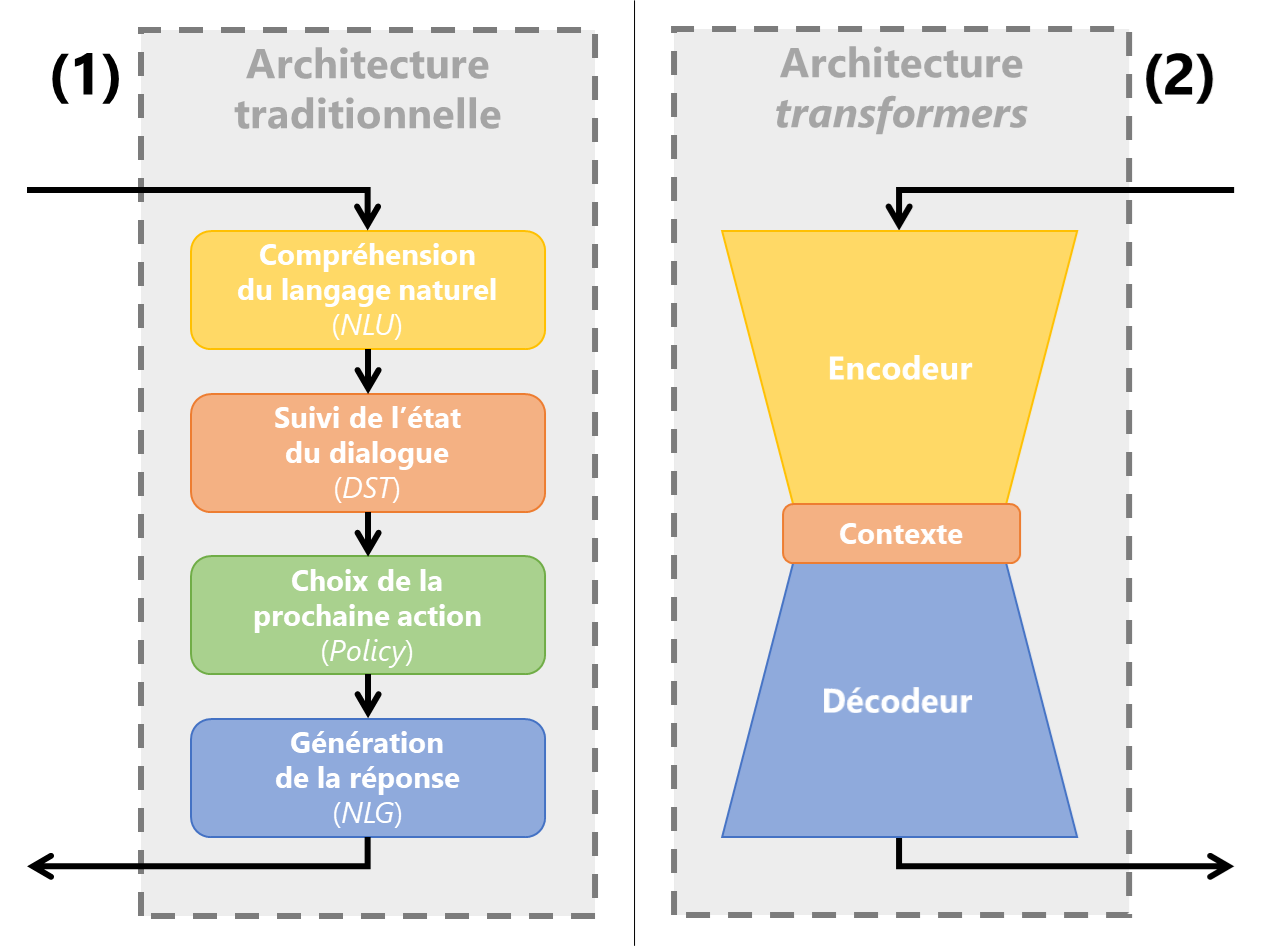
\includegraphics[width=0.90\textwidth]{figures/annexe-chatbots-architectures}
			\caption{
				Schéma illustrant les deux approches principales de conception d'un assistant conversationnel :
				\textbf{(1)} représente les \textbf{approches \textit{task-oriented}} à l'aide d'une architecture manipulant des états de dialogue ;
				\textbf{(2)} représente les \textbf{approches \textit{chat-oriented}} à l'aide d'une architecture à base de \textit{transformers}, encodant et décodant numériquement le dialogue et son contexte.
			}
			\label{figure:B.2-ANNEXE-CHATBOT-APPROCHES}
		\end{figure}
		
		
		%%%
		%%% Subsection B.2.1: Approches \textit{task-oriented}.
		%%%
		\newpage
		\subsection{Approches \textit{task-oriented}}
		\label{annex:B.2.1-ANNEXE-CHATBOTS-APPROCHES-TASK-ORIENTED}
		
			% Description.
			Les \textbf{approches orientées par tâches} (\textit{task-oriented}) considèrent la conversation comme une succession d'étapes menant à une action précise : le système est donc conçu pour collecter les informations nécessaires et interagir avec un moteur d'actions dans le but d'accomplir un objectif.
			Ces approches reposent généralement sur une modélisation explicite du parcours utilisateur, permettant ainsi de s'assurer de l'exécution pas à pas des actions intermédiaires de la tâche demandée.
			
			% Achitecture.
			La \textsc{Figure~\ref{figure:B.2-ANNEXE-CHATBOT-APPROCHES}} \textbf{(1)} représente l'architecture traditionnellement utilisée pour concevoir ce type d'assistants.
			Cette architecture est composée de éléments suivants :
			\begin{itemize}
				% NLU.
				\item le \textcolor{colorCarrotOrange}{\textbf{\texttt{NLU}}} (\textit{Natural Language Understanding}) :
					ce composant utilise un ensemble de concepts pour interpréter le dialogue de manière symbolique.
					Cette modélisation du dialogue, généralement implémentée à l'aide de méthodes supervisées, repose sur des détections de \textit{domaines} (\textit{thématique générale traitée}), des détections de \textit{sentiments} (\textit{positif, négatif ou neutre}), des détections d'\textit{intentions} (\textit{action exprimée par l'utilisateur, manifesté par le verbe d'action}), ou encore des extractions d'\textit{entités} (\textit{ensemble de mentions textuelles pertinentes}) (voir \cite{adamopoulou-moussiades:2020:overview-chatbot-technology}) ;
				% DST.
				\item le \textcolor{colorDarkPastelGreen}{\textbf{\texttt{DST}}} (\textit{Dialogue State Tracking}) :
					ce composant utilise les concepts détectés précédemment par le \texttt{NLU} (\textit{domaine}, \textit{sentiment}, \textit{intentions}, \textit{entités}) pour déterminer ou mettre à jour l'état de la conversation, et ainsi définir les actions possibles à partir de l'état en cours ;
				% PL.
				\item la \textcolor{colorDarkPastelGreen}{\textbf{\texttt{PL}}} (\textit{Policy Learning}) : 
					ce composant choisit la prochaine action de l'assistant parmi celle autorisée par le \texttt{DST} pour l'état en cours.
					Ce choix peut être réalisé à l'aide d'un ensemble de règles, d'un apprentissage supervisé ou encore d'un apprentissage par renforcement (voir \cite{brabra-etal:2022:dialogue-management-conversational}) ;
				% NLG.
				\item la \textcolor{colorSilverLakeBlue}{\textbf{\texttt{NLG}}} (\textit{Natural Language Generation}) :
					ce dernier composant affiche une réponse à l'utilisateur qui soit en adéquation avec l'action choisie par la \texttt{PL}.
					Cette réponse peut être paramétrée à l'avance ou être générée à la volée.
			\end{itemize}
			
			
			% Avantages et inconvénients.
			Cette approche est rudimentaire mais efficace, et elle est par conséquent fréquemment utilisée pour concevoir des assistants conversationnels dans un cadre industriel.
			\begin{itemize}
				\item[\textcolor{colorDarkPastelGreen}{\textcolor{colorDarkPastelGreen}{\faThumbsUp}}] Au sujet des avantages :
					% Implémentation facile.
					les différents composants de l'architecture sont simples à implémenter et à maintenir
					(\textit{ces différentes briques sont indépendantes et ont des fonctionnalités bien précises}) ;
					% Paramétrage facile.
					de nouvelles règles de dialogues peuvent facilement être ajoutées dans le système
					(\textit{du moins si les processus de ces tâches sont bien documentés}) ;
					% Mise sous contrôle.
					il est facile de contrôler le comportement de l'assistant
					(\textit{il suffit de restreindre les actions possibles dans le \texttt{DST}, de figer le choix de la \texttt{PL}, ou encore de déterminer à l'avance chaque réponse de la \texttt{NLG}}) ;
					% Infrastructure légère.
					cette architecture simple consomme peu de ressources en production (\textit{les modèles de détections et la gestion du dialogue peuvent tourner sur \texttt{CPU}}).
				\item[\textcolor{colorDarkPastelRed}{\textcolor{colorDarkPastelRed}{\faThumbsDown}}] Au sujet des inconvénients :
					% Couts initiaux.
					les coûts initiaux peuvent être importants (\textit{notamment en ce qui concerne la collecte et la modélisation des données d'apprentissage, ou encore la définition des parcours de dialogue pour des tâches non documentées}) ;
					% Modélisation sensible aux erreurs.
					la compréhension du langage est limitée (\textit{certaines erreurs ou ambiguïtés de langage rendent les détections du \texttt{NLU} non adaptées ou non performantes}) ;
					% Peu flexible.
					le dialogue est très peu flexible, et le périmètre de l'assistant est réduit à ce qui est modélisé (\textit{le dialogue peut être bloqué ou rejeté si aucune règle n'est prévue pour la demande de l'utilisateur ou pour l'état courant}).
			\end{itemize}
			
			\newpage
			
			% Exemple fictif.
			\begin{leftBarExamples}
				Pour illustrer nos propos, analysons la demande fictive suivante :
				\begin{quote}
					\begin{center}
						\textguillemets{\textit{
							Je veux réserver un billet de train pour Strasbourg.
						}}
					\end{center}
				\end{quote}
				\begin{itemize}
					\item le \texttt{NLU} pourrait détecter le domaine "\texttt{voyage}", l'intention "\texttt{réservation}" et les entités "$\textit{billet de train}_{\texttt{(produit)}}$" et "$\textit{Strasbourg}_{\texttt{(gare\_destination)}}$" ;
					\item le \texttt{DST} pourrait établir l'objectif de réserver un train, mais que les informations \texttt{(date\_départ)} et \texttt{(gare\_départ)} sont manquantes ;
					\item la \texttt{PL} pourrait décider de demander d'abord le complément d'information sur la gare de départ (\textit{et demandera la prochaine information plus tard}) ;
					\item la \texttt{NLG} pourrait sortir une phrase de réponse prédéfinie pour demander le complément d'information à l'utilisateur.
				\end{itemize}
			\end{leftBarExamples}
				
			% Exemples réels
			\begin{leftBarExamples}
				Nous pouvons citer les projets ou outils suivants :
				\begin{itemize}
					\item \texttt{RASA} (\cite{bocklisch-etal:2017:rasa-open-source}) et \texttt{WATSON} (\cite{hoyt-etal:2016:ibm-watson-analytics}) sont deux moteurs de dialogue basés sur une approche symbolique et manipulant des intentions et des entités ;
					\item \texttt{Assistant Virtuel SNCF} (\cite{sncf:2018:agent-virtuel-sncf}), \texttt{Google Assistant} (\cite{google:2016:google-assistant-your}) et \texttt{Alexa} (\cite{alexa-internet:2018:keyword-research-competitor}) sont des assistants connus pour être orientés par tâches, les deux derniers pouvant même être paramétrables par l'utilisateur final pour ses usages en domotiques ;
					\item \cite{yan-etal:2017:building-taskoriented-dialogue} décrivent un projet de conception d'un assistant conversationnel pour du commerce en ligne.
				\end{itemize}
			\end{leftBarExamples}
		
		
		%%%
		%%% Subsection B.2.2: Approches \textit{chat-oriented}.
		%%%
		\subsection{Approches \textit{chat-oriented}}
		\label{annex:B.2.2-ANNEXE-CHATBOTS-APPROCHES-CHAT-ORIENTED}
			
			% Description.
			Les \textbf{approches axées sur le dialogue} (\textit{chat-oriented} ou \textit{non-task-oriented}) sont utilisées pour favoriser des conversations ouvertes avec les utilisateur : le système n'est donc pas conçu pour répondre à un besoin spécifique, mais plutôt pour être en mesure de discuter avec un utilisateur sur des thématiques générales et de rebondir à chacun de ses messages de manière fluide .
			Afin de capturer la vaste diversité du langage, ces approches reposent majoritairement sur les capacités du \textit{Deep Learning}, notamment pour concevoir des modèles de langage permettant de capturer et de reproduire des séquences de phrases (voir \cite{ni-etal:2022:recent-advances-deep} et \cite{kumar-etal:2016:ask-me-anything}).
			
			% Achitecture.
			La \textsc{Figure~\ref{figure:B.2-ANNEXE-CHATBOT-APPROCHES}} \textbf{(2)} correspond à l'architecture \textit{transformers} (\cite{uszkoreit:2017:transformer-novel-neural}), communément utilisée pour représenter ce type d'assistants.
			Cette architecture est composée de deux réseaux de neurones :
			\begin{itemize}
				% Encodeur.
				\item un \textcolor{colorCarrotOrange}{\textbf{\texttt{encodeur}}} :
					ce premier réseau a pour objectif de traduire les séquences de mots du texte de l'utilisateur en une représentation numérique abstraite ;
				% Decodeur.
				\item le \textcolor{colorSilverLakeBlue}{\textbf{\texttt{décodeur}}} :
					ce second réseau a pour objectif de traiter la représentation numérique produite par l'encodeur dans le but de générer des séquences de mots pour former la réponse ;
				% Contexte.
				\item entre les deux, un \textcolor{colorDarkPastelGreen}{\textbf{\texttt{vecteur de contexte}}} :
					ce vecteur permet de maintenir la continuité de la conversation entre deux échanges.
					L'encodeur se charge de mettre à jour le contexte tandis que le décodeur l'utilise pour adapter la génération de son texte.
			\end{itemize}
			
			
			% Avantages et inconvénients.
			Cette approche est plus difficile à mettre en place qu'une approche symbolique, mais elle dispose d'un plus grand potentiel.
			\begin{itemize}
				\item[\textcolor{colorDarkPastelGreen}{\textcolor{colorDarkPastelGreen}{\faThumbsUp}}] Au sujet des avantages :
					% Grande flexibilité.
					par conception, le système peut s'adapter à de nombreuses situations et offrir une expérience agréable à l'utilisateur
					(\textit{aucun blocage de l'état du dialogue, possibilité de personnaliser le dialogue, gestion plus simple de l'ambiguïté et des émotions, ...}) ;
					% Compréhension du langage.
					il n'a pas besoin d'interpréter le langage à l'aide d'une modélisation abstraite
					(\textit{cette interprétation est déduite de l'immense volume de textes utilisés à l’entraînement}) ;
					% Autres propriétés
					en utilisant des larges modèles de langage, des propriétés intéressantes peuvent apparaître
					(\textit{capable de consulter un très large champ de connaissances, de résumer et traduire un texte, de résoudre un calcul, d'effectuer une tâche d'analyse ou de déduction, de générer un code informatique, ...}).
				\item[\textcolor{colorDarkPastelRed}{\textcolor{colorDarkPastelRed}{\faThumbsDown}}] Au sujet des inconvénients :
					% Coûts techniques imports.
					les coûts d'entraînement et d'inférence du modèle sont conséquents
					(\textit{besoin d'une immense quantité de données pour l'apprentissage, besoin de \texttt{GPU} et d'une infrastructure technique conséquente, ...}) ;
					% Réponses erronées.
					le décodeur peut générer des contenus inexactes, erronés ou offensant
					(\textit{imprécisions, fausses informations, hallucinations, réponse biaisée ou discriminatoire, ...}) ;
					la reproduction des données utilisées pour l'entraînement questionne le respect des droits d'auteur et expose potentiellement des données privées ou confidentielles
					(\textit{capacités à reproduire des passages entiers de livres, à trouver des numéros de cartes bancaires ou des clés d'activation de logiciel issus de fuites de bases de données, ...}) ;
					% Mise sous contrôle.
					la mise sous contrôle de l'assistant est difficile voire impossible
					(\textit{manque de visibilité et d'explicabilité concernant le comportement du modèle, peu de leviers d'action direct, recours à une annotation de masse par ressenti utilisateur, ...}).
			\end{itemize}
			
			% Exemples.
			\begin{leftBarExamples}
				Nous pouvons citer les projets ou outils suivants :
				\begin{itemize}
					\item \texttt{ChatGPT} (\cite{openai:2023:chatgpt}), \texttt{BARD} (\cite{google:2023:bard-chat-based}) et \texttt{LLAMA2} (\cite{touvron-etal:2023:llama-open-foundation}) sont trois solutions basées sur des larges modèles de langage permettant de discuter de presque tous les domaines ainsi que de réaliser de très nombreuses tâches ;
					\item \cite{kaddour-etal:2023:challenges-applications-large} détaillent une longue liste d'inconvénients et de défis pour l'utilisation de larges modèles de langage.
				\end{itemize}
			\end{leftBarExamples}
	
	
	%%%%%--------------------------------------------------------------------
	%%%%% Annexe B.3: Dilemme de conception et approches hybrides.
	%%%%%--------------------------------------------------------------------
	\newpage
	\section{Dilemme de conception et approches hybrides}
	\label{annex:B.3-ANNEXE-CHATBOTS-DILEMME}
		
		%%% Introduction: Description du dilemme.
		Dans la section précédente, nous avons pu voir que deux approches de conception se distinguent :
		d'une part, il y a l'approche \textit{task-oriented}, basée sur une gestion symbolique du dialogue et permettant facilement de contrôler le comportement de l'assistant ;
		d'autre part, il y a l'approche \textit{chat-oriented}, basée sur un encodage/décodage numérique de la conversation et permettant une grande flexibilité dans les échanges avec l'utilisateur.
		Cependant, chaque approche possède les inconvénients de l'autre approche :
		en effet, l'approche \textit{task-oriented} est plutôt rigide, tandis que l'approche \textit{chat-oriented} est sensible aux dérives de comportement et aux risques d'hallucinations.
		Nous nous trouvons donc face à un dilemme de conception : \textbf{voulons-nous privilégier la fluidité du dialogue ou le contrôle du comportement de l'assistant ?}
		
		
		%%% Notes: Questionnement sur le niveaux d'automatisation.
		Ce choix cornélien questionne le \textbf{niveau d'automatisation} que nous sommes prêts à déléguer à la machine.
		
		\begin{leftBarAuthorOpinion}
			% Dix niveaux d'automatisation.
			Pour estimer un \textbf{degré d'automatisation}, \cite{sheridan-verplank:1978:human-computer-control} identifient \textbf{dix niveaux} :
			\begin{itemize}
				\item de \textguillemets{la machine n'offre aucune assistance, l'opérateur doit choisir l'action à faire et la réaliser lui-même} (\textit{niveau 1 : automatisation nulle}) ;
				\item à \textguillemets{la machine s'occupe de tout (analyse, choix et réalisation de l'action) sans consultation au préalable de l'opérateur ni information sur le déroulement de la tâche} (\textit{niveau 10 : automatisation totale}).
			\end{itemize}
			
			% Quatre fonctions à automatisées.
			En plus de cette proposition en dix niveaux d'automatisation, \cite{parasuraman-etal:2000:model-types-levels} proposent une analyse selon \textbf{quatre aspects} :
			\begin{itemize}
				\item l'acquisition de l'information (\textit{à quel point la machine collecte et sélectionne les informations pertinentes à porter à l'attention de l'opérateur ?}) ;
				\item l'analyse de l'information (\textit{à quel point la machine participe à l'examen des informations dans le but de proposer les actions possibles à réaliser ?}) ;
				\item la prise de décision (\textit{à quel point la machine choisit l'action à réaliser à la place de l'opérateur ?}) ;
				\item l'implémentation de l'action (\textit{à quel point la machine réalise l'action et informe l'opérateur des résultats ?}).
			\end{itemize}
			
			%%% Aplicationa aux chatbots.
			Nous pouvons d'ailleurs faire des parallèles avec l'architecture des assistants conversationnels :
			\begin{itemize}
				\item l'acquisition de l'information correspond au \textcolor{colorCarrotOrange}{\textbf{\texttt{NLU}}} ou à l'\textcolor{colorCarrotOrange}{\textbf{\texttt{encodeur}}} ;
				\item l'analyse de l'information et la prise de décision correspondent aux \textcolor{colorDarkPastelGreen}{\textbf{\texttt{DST}}}/\textcolor{colorDarkPastelGreen}{\textbf{\texttt{PL}}} ou à la manipulation du \textcolor{colorDarkPastelGreen}{\textbf{\texttt{vecteur de contexte}}} ;
				\item l'implémentation de l'action correspond à la \textcolor{colorSilverLakeBlue}{\textbf{\texttt{NLG}}} ou au \textcolor{colorSilverLakeBlue}{\textbf{\texttt{décodeur}}}.
			\end{itemize}
			De ce fait, les choix de conception de l'assistant reviennent à définir quels composants doivent être rigides (\textit{gestion de règles}), entraînés (\textit{apprentissage supervisé, ...}) ou totalement délégués à la machine (\textit{modèles de langage, ...}).
		\end{leftBarAuthorOpinion}
		
		%%% Approches hybrides.
		\newpage
		Pour résoudre ce dilemme de conception, \textbf{diverses approches hybrides peuvent être mises en oeuvre} :
		\begin{itemize}
			\item si nous voulons \textbf{plus de fluidité} dans la conversation (\textit{pour améliorer l'ergonomie utilisateur, pour permettre de discuter de sujets plus généraux, ...}), nous intégrerons davantage de composants issus d'une approche \textit{chat-oriented}, acceptant en échange de \textbf{déléguer} la gestion du dialogue et/ou la génération de réponse à la machine ;
			\item à l'inverse, si nous avons besoin d'un \textbf{contrôle plus fort} (\textit{pour assurer la sécurité des actions réaliser, pour garantir l'image de la marque, pour éviter les scandales, ...}), nous nous tournerons davantage vers l'utilisation de composants modélisant une approche symbolique du dialogue, permettant ainsi de \textbf{limiter la machine} dans ses possibilités.
		\end{itemize}
			
		% Exemples.
		\begin{leftBarExamples}
			Nous dressons une liste non exhaustives d'approches hybrides :
			\begin{itemize}
				\item la compréhension du langage naturel à l'aide de détection de concepts (\texttt{NLU}) peut être améliorée en utilisant les capacités d'un large modèle de langage (voir \texttt{RASA v3.6+} par \cite{bocklisch-etal:2017:rasa-open-source}) ou en réutilisant les représentations vectorielles produites par l'encodeur (\textit{embeddings}) ;
				\item le moteur de dialogue d'une approche \textit{task-oriented} (\texttt{DST} et \texttt{PL}) peut être entraîné par renforcement dans le but d'améliorer la prise de décision et de rendre les étapes de dialogue plus flexibles (voir \cite{chen-etal:2017:survey-dialogue-systems} et \cite{brabra-etal:2022:dialogue-management-conversational}) ;
				\item le décodeur d'une approche \textit{chat-oriented} peut être utilisé pour la génération de réponse d'un assistant \textit{task-oriented} (\texttt{NLG}), permettant afin d'améliorer la qualité de ses réponses (voir \cite{gao-etal:2018:neural-approaches-conversational} et \cite{chen-etal:2017:survey-dialogue-systems}) ;
				\item il est possible de se baser sur une tâche de recherche d'information dans une base documentaire pour limiter les hallucinations lors de la génération de réponse (voir \cite{shuster-etal:2021:retrieval-augmentation-reduces} et \cite{zhang-etal:2016:neural-information-retrieval}).
			\end{itemize}
		\end{leftBarExamples}


%%%%%--------------------------------------------------------------------
%%%%% Annexe X: ANNEXE TECHNIQUE
%%%%%--------------------------------------------------------------------
%\Annex{Annexe technique}
%\label{annex:X-ANNEXE-TECHNIQUE}

	% INTRODUCTION DE L'ANNEXE.
	% ??

	% TABLE DES MATIÈRES DE L'ANNEXE.
	%\minitoc

	%%%%%--------------------------------------------------------------------
	%%%%% Annexe X.1: Méthodes d'évaluation d'un \textit{clustering}.
	%%%%%--------------------------------------------------------------------
	%\section{Méthodes d'évaluation d'un \textit{clustering}}
	%\label{annex:X.1-TECHNIQUE-EVALUATION-CLUSTERING}

\todo[inline]{ANNEXE: v-measure, fmc}



%%%%%--------------------------------------------------------------------
%%%%% Annexe X: ANNEXE DEVELOPPEMENTS
%%%%%--------------------------------------------------------------------
%\Annex{Développements Python}
%\label{annex:X-ANNEXE-DEVELOPPEMENTS}

	% INTRODUCTION DE L'ANNEXE.
	% ??

	% TABLE DES MATIÈRES DE L'ANNEXE.
	%\minitoc

	%%%%%--------------------------------------------------------------------
	%%%%% Annexe X.1: Interactive Clustering GUI.
	%%%%%--------------------------------------------------------------------
	%\section{Interactive Clustering GUI}
	%\label{annex:X.1-DEVELOPPEMENTS-INTERACTIVE-CLUSTERING-GUI}
	
\todo[inline]{ANNEXE: packages python, captures écran application}


%%%%%%%%%%%%%%%%%%%%%%%%%%%%%%%%%%%%%%%%%%%%%%%%%%%%%%%%%%%%%%%%%%%%%%%
%%%%% DIVERS
%%%%%%%%%%%%%%%%%%%%%%%%%%%%%%%%%%%%%%%%%%%%%%%%%%%%%%%%%%%%%%%%%%%%%%%

\PutLineInToc
\DontFrameChaptersInToc

%%%%%--------------------------------------------------------------------
%%%%% Bibliographie
%%%%%--------------------------------------------------------------------

%%% Affichage de la bibliographie:
\printbibliography

% Use "\nocite{*}" to add all .bib file.
% Use this command to see which references are note cited.

%%%%%--------------------------------------------------------------------
%%%%% Liste des TODOs
%%%%%--------------------------------------------------------------------

%%% Génère la liste des choses à faire:
\listoftodos[Liste des TODOs]

%%%%%--------------------------------------------------------------------
%%%%% Liste des figures
%%%%%--------------------------------------------------------------------

%%% Génère la liste des figures:
\renewcommand{\listfigurename}{Liste des figures}
\listoffigures

%%%%%--------------------------------------------------------------------
%%%%% Liste des tableaux
%%%%%--------------------------------------------------------------------

%%% Génère la liste des tableaux:
\renewcommand{\listtablename}{Liste des tableaux}
\listoftables

%%%%%--------------------------------------------------------------------
%%%%% Liste des algorithmes
%%%%%--------------------------------------------------------------------

%%% Génère la liste des algorithmes:
%\renewcommand{\listalgorithmname}{Liste des algorithmes}
\renewcommand{\listalgorithmcfname}{Liste des algorithmes}
\listofalgorithms  % ERROR TABLE MATIERES

%%%%%--------------------------------------------------------------------
%%%%% Liste des codes
%%%%%--------------------------------------------------------------------

%%% Génère la liste des codes:
\renewcommand{\lstlistlistingname}{Liste de codes informatiques}
\lstlistoflistings

%%%%%--------------------------------------------------------------------
%%%%% Glossaire
%%%%%--------------------------------------------------------------------

%%% Affichage du glossaire:
\printglossaries

%%%%%--------------------------------------------------------------------
%%%%% Index
%%%%%--------------------------------------------------------------------

%%% Affichage de l'index:
\WriteThisInToc
\PrintIndex

\end{document}